%--------------------------------------------------------------------------
%
%  OOD Project
%  Arno
%  By: Saba Hashemi, Amirmahdi Namjoo, Mostafa Ojaghi, Alireza Tajmirriahi
%
%--------------------------------------------------------------------------

%--------------------------------------------------------------------------
%
% Template is based on LaTeX Thesis Template (v2.2)
%  By: Hamid Zarrabi-Zadeh
%
%  Contributors:
%      Ehsan Emamjomeh-Zadeh
%      Omid Gheibi
%
%--------------------------------------------------------------------------


\documentclass[oneside,a4paper,12pt]{book}
 

% -------------------------------------------------------
%  Common Styles and Formattings
% -------------------------------------------------------


\usepackage{amssymb,amsmath}
\usepackage[colorlinks,linkcolor=blue,citecolor=blue]{hyperref}
\usepackage[usenames,dvipsnames]{pstricks}
\usepackage{graphicx,subfigure,wrapfig}
\usepackage{geometry,fancyhdr}
\usepackage[mathscr]{euscript}
\usepackage{multicol}
\usepackage{array}
\usepackage{enumitem}
\usepackage{setspace}

\usepackage{placeins}

\usepackage{longtable}


\usepackage{algorithmicx,algorithm}

\usepackage[localise=on,extrafootnotefeatures]{xepersian}
\usepackage[noend]{algpseudocode}


%------------------------ Algorithm ------------------------------------

\newenvironment{الگوریتم}[1]
	{\bigskip\bigskip\begin{algorithm}\caption{#1} \label{الگوریتم: #1}\vspace{0.5em}\begin{algorithmic}[1]}
	{\end{algorithmic}\vspace{0.5em}\end{algorithm}\bigskip}
	

\renewcommand{\algorithmicfor}{{به ازای}}
\renewcommand{\algorithmicwhile}{{تا وقتی}}
\renewcommand{\algorithmicdo}{\hspace{-.2em}:}
\renewcommand{\algorithmicif}{{اگر}}
\renewcommand{\algorithmicthen}{\hspace{-.2em}:}
\renewcommand{\algorithmicelse}{{در غیر این صورت:}}
%\renewcommand{\algorithmicelsif}{{در غیر این صورت اگر: }}
\renewcommand{\algorithmicreturn}{{برگردان}}
\renewcommand{\algorithmiccomment}[1]{$\triangleleft$ \emph{#1}}
\renewcommand{\algorithmicrequire}{\textbf{ورودی:}}
\renewcommand{\algorithmicensure}{\textbf{خروجی:}}

\newcommand{\اگر}{\If}
\newcommand{\وگرنه}{\Else}
\newcommand{\وگر}{\ElsIf}
\newcommand{\پایان‌اگر}{\EndIf}
\newcommand{\به‌ازای}{\For}
\newcommand{\پایان‌به‌ازای}{\EndFor}
\newcommand{\تاوقتی}{\While}
\newcommand{\پایان‌تاوقتی}{\EndWhile}
\newcommand{\دستور}{\State}
\newcommand{\دستورک}{\Statex}
\newcommand{\توضیحات}{\Comment}
\newcommand{\برگردان}{\Return}
\renewcommand{\ورودی}{\Require}
\newcommand{\خروجی}{\Ensure}



% -------------------- Page Layout --------------------


\newgeometry{top=3.5cm,bottom=3.5cm,left=2.5cm,right=3cm,headheight=25pt}

\renewcommand{\baselinestretch}{1.4}
\linespread{1.6}
\setlength{\parskip}{0.45em}

\fancyhf{}
\rhead{\leftmark}
\lhead{\thepage}


% -------------------- Fonts --------------------

\settextfont[
Scale=1.09,
Extension=.ttf, 
Path=styles/fonts/,
BoldFont=XB NiloofarBd,
ItalicFont=XB NiloofarIt,
BoldItalicFont=XB NiloofarBdIt
]{XB Niloofar}

\setdigitfont[
Scale=1.09,
Extension=.ttf, 
Path=styles/fonts/,
BoldFont=XB NiloofarBd,
ItalicFont=XB NiloofarIt,
BoldItalicFont=XB NiloofarBdIt
]{XB Niloofar}

\defpersianfont\sayeh[
Scale=1,
Path=styles/fonts/
]{XB Kayhan Pook}


% -------------------- Styles --------------------


\SepMark{-}
\renewcommand{\labelitemi}{$\small\bullet$}



% -------------------- Environments --------------------


\newtheorem{قضیه}{قضیه‌ی}[chapter]
\newtheorem{لم}[قضیه]{لم}
\newtheorem{ادعا}[قضیه]{ادعای}
\newtheorem{مشاهده}[قضیه]{مشاهده‌ی}
\newtheorem{نتیجه}[قضیه]{نتیجه‌ی}
\newtheorem{مسئله}{مسئله‌ی}[chapter]
\newtheorem{تعریف}{تعریف}[chapter]
\newtheorem{مثال}{مثال}[chapter]


\newenvironment{اثبات}
{\begin{trivlist}\item[\hskip\labelsep{\em اثبات.}]}
	{\leavevmode\unskip\nobreak\quad\hspace*{\fill}{\ensuremath{{\square}}}\end{trivlist}}

\newenvironment{alg}[2]
{\begin{latin}\settextfont[Scale=1.0]{Times New Roman}
		\begin{algorithm}[t]\caption{#1}\label{algo:#2}\vspace{0.2em}\begin{algorithmic}[1]}
			{\end{algorithmic}\vspace{0.2em}\end{algorithm}\end{latin}}


% -------------------- Titles --------------------


\renewcommand{\listfigurename}{فهرست شکل‌ها}
\renewcommand{\listtablename}{فهرست جدول‌ها}
\renewcommand{\bibname}{\rl{{مراجع}\hfill}} 


% -------------------- Commands --------------------


\newcommand{\IN}{\ensuremath{\mathbb{N}}} 
\newcommand{\IZ}{\ensuremath{\mathbb{Z}}} 
\newcommand{\IQ}{\ensuremath{\mathbb{Q}}} 
\newcommand{\IR}{\ensuremath{\mathbb{R}}} 
\newcommand{\IC}{\ensuremath{\mathbb{C}}} 

\newcommand{\set}[1]{\left\{ #1 \right\}}
\newcommand{\seq}[1]{\left< #1 \right>}
\newcommand{\ceil}[1]{\left\lceil{#1}\right\rceil}
\newcommand{\floor}[1]{\left\lfloor{#1}\right\rfloor}
\newcommand{\card}[1]{\left|{#1}\right|}
\newcommand{\setcomp}[1]{\overline{#1}}
\newcommand{\provided}{\,:\,}
\newcommand{\divs}{\mid}
\newcommand{\ndivs}{\nmid}
\newcommand{\iequiv}[1]{\,\overset{#1}{\equiv}\,}
\newcommand{\imod}[1]{\allowbreak\mkern5mu(#1\,\,\text{پیمانه‌ی})}

\newcommand{\poly}{\mathop{\mathrm{poly}}}
\newcommand{\polylog}{\mathop{\mathrm{polylog}}}
\newcommand{\eps}{\varepsilon}

\newcommand{\lee}{\leqslant}
\newcommand{\gee}{\geqslant}
\renewcommand{\leq}{\lee}
\renewcommand{\le}{\lee}
\renewcommand{\geq}{\gee}
\renewcommand{\ge}{\gee}

\newcommand{\مهم}[1]{\textbf{#1}}
\renewcommand{\برچسب}{\label}

\newcommand{\REM}[1]{}
\renewcommand{\حذف}{\REM}
\newcommand{\لر}{\lr}
\newcommand{\کد}[1]{\lr{\tt #1}}
\newcommand{\پاورقی}[1]{\footnote{\lr{#1}}}



% -------------------- Dictionary --------------------


\newcommand{\dicalphabet}[1]{
	\begin{minipage}{\columnwidth}
		\centerline{\noindent\textbf{\large #1 }}
		\vspace{.5em}
	\end{minipage}
	\nopagebreak[4]
}

\newcommand{\dic}[2]{\noindent  #2 \dotfill  \lr{#1} \\ }


% ------------------------------ Images and Figures --------------------------

\graphicspath{{figs/}}
\setlength{\intextsep}{0pt}  % for float boxes
\renewcommand{\psscalebox}[1]{}  % for LaTeX Draw

\newcommand{\floatbox}[2]
{\begin{wrapfigure}{l}{#1}
		\centering #2 \end{wrapfigure}}

\newcommand{\centerfig}[2]
{\centering\scalebox{#2}{\input{figs/#1}}}

\newcommand{\fig}[3]
{\floatbox{#3}{\centerfig{#1}{#2}}}

\newcommand{\centerimg}[2]
{\vspace{1em}\begin{center}\includegraphics[width=#2]{figs/#1}\end{center}\vspace{-1.5em}}

\NewDocumentCommand{\img}{m m o}
{\begin{wrapfigure}{l}{\IfValueTF{#3}{#3}{#2}}
		\centering\includegraphics[width=#2]{figs/#1}\end{wrapfigure}}




\newcommand{\usecase}[9]{
	\def\tempa{#1}%
	\def\tempb{#2}%
	\def\tempc{#3}%
	\def\tempd{#4}%
	\def\tempe{#5}%
	\def\tempf{#6}%
	\def\tempg{#7}%
	\def\temph{#8}%
	\def\tempi{#9}%

\usecasecontinue
}

\newcommand\usecasecontinue[1]{%
	\begin{singlespace}
		\begin{table}[ht!]
			\setlength\extrarowheight{-5pt}
			\centering
			\begin{tabular}{|p{0.18\linewidth}|p{0.82\linewidth}|} 
				\hline
				\multicolumn{2}{|c|}{مورد کاربرد: {\tempa}}  \\ 
				\hline
				شناسه           &     \tempb                   \\ 
				\hline
				توضیح مختصر     &     \tempc                   \\ 
				\hline
				کنشگرهای اولیه  &     \tempd                   \\ 
				\hline
				کنشگرهای ثانویه &    \tempe                    \\ 
				\hline
				پیش‌نیازها      &     \tempf                  \\ 
				\hline
				روند اصلی       &    \tempg                    \\ 
				\hline
				پس‌نیاز‌ها      &     \temph                   \\ 
				\hline
				روند جایگزین    &  \tempi            \\
				\hline
			\end{tabular}
			\caption{#1}	
		\end{table}
	\end{singlespace}
\FloatBarrier
\newpage
}



\newcommand{\alternativeflow}[8]{
	\def\tempa{#1}%
	\def\tempb{#2}%
	\def\tempc{#3}%
	\def\tempd{#4}%
	\def\tempe{#5}%
	\def\tempf{#6}%
	\def\tempg{#7}%
	\def\temph{#8}%
	
	\alternativeflowcontinue
}

\newcommand\alternativeflowcontinue[1]{%
	\begin{singlespace}
		\begin{table}[ht!]
			\setlength\extrarowheight{-5pt}
			\centering
			\begin{tabular}{|p{0.18\linewidth}|p{0.82\linewidth}|} 
				\hline
				\multicolumn{2}{|c|}{روند جایگزین: {\tempa}}  \\ 
				\hline
				شناسه           &     \tempb                   \\ 
				\hline
				توضیح مختصر     &     \tempc                   \\ 
				\hline
				کنشگرهای اولیه  &     \tempd                   \\ 
				\hline
				کنشگرهای ثانویه &    \tempe                    \\ 
				\hline
				پیش‌نیازها      &     \tempf                  \\ 
				\hline
				روند اصلی       &    \tempg                    \\ 
				\hline
				پس‌نیاز‌ها      &     \temph                   \\ 
				\hline
			\end{tabular}
			\caption{#1}	
		\end{table}
	\end{singlespace}
\FloatBarrier
\newpage
	
}


\newcommand{\glossaryTitle}[1]{
	\hline
	\hline
	\multicolumn{2}{|c|}{}  \\
	\multicolumn{2}{|c|}{\linebreak \LARGE\textbf{{#1}}}  \\
	\multicolumn{2}{|c|}{}  \\ \hline \hline
	
}

\newcommand{\glossaryEntry}[4]{
	#1
	&
	\textbf{معنا} \hspace{1.53cm} #2
	
	\textbf{مترادف} \hspace{1cm} #3
	
	\textbf{متشابه}\hspace{1.28cm} #4
	\\
	\hline
	
}

\newcommand{\calendarEntry}[6]{
		#1 & #2 & $#3$ & ۱۴۰۱/#4 & ۱۴۰۱/#5 & #6\\
		\hline
}


\newcommand{\changelogEntry}[2]{
	 ۱۴۰۱/#1 & #2\\
	\hline
}




% -------------------------------------------------------
%  Custom Definitions
% -------------------------------------------------------


\newcommand{\OPT}{\ensuremath{\mathop{\mathrm{OPT}}}}
\newcommand{\APX}{\ensuremath{\mathop{\mathrm{APX}}}}
\newcommand{\ALG}{\ensuremath{\mathop{\mathrm{ALG}}}}



\begin{document}
	% -------------------- Front Pages --------------------
	
	%\pagenumbering{alph}
	
	
% -------------------------------------------------------
%  Thesis Information
% -------------------------------------------------------

\newcommand{\ThesisType}
{پروژه‌ی درس طراحی شی‌گرا}
\newcommand{\ThesisTitle}
{مجموعه مستندات سیستم ...}
\newcommand{\ThesisAuthor}
{مصطفی اوجاقی، علیرضا تاج‌میرریاحی، امیرمهدی نامجو، صبا هاشمی}
\newcommand{\ThesisSupervisor}
{جناب آقای دکتر رامسین}
\newcommand{\ThesisAdvisor}
{استاد مشاور}
\newcommand{\ThesisExaminer}
{استاد ممتحن}
\newcommand{\ThesisDate}
{بهار و تابستان ۱۴۰۱}
\newcommand{\ThesisDepartment}
{دانشکده‌ی مهندسی کامپیوتر}
\newcommand{\ThesisMajor}
{}
\newcommand{\ThesisUniversity}
{دانشگاه صنعتی شریف}


% -------------------------------------------------------
%  English Information
% -------------------------------------------------------

\newcommand{\EnglishThesisType}{M.Sc. Thesis}

\newcommand{\EnglishThesisTitle}{A Standard Template for Typesetting Theses in Persian}

\newcommand{\EnglishThesisAuthor}{Hamid Zarrabi-Zadeh}

\newcommand{\EnglishThesisSupervisor}{Dr. Supervisor}

\newcommand{\EnglishThesisDate}{September 2020}

\newcommand{\EnglishThesisDepartment}{Department of Computer Engineering}

\newcommand{\EnglishThesisUniversity}{Sharif University of Technology}

	
\pagestyle{empty}

\begin{center}


\includegraphics[scale=0.2]{front/template/images/logo.png}

\begin{large}

\vspace{-0.2cm}
\ThesisUniversity \\[-0.3em]
\ThesisDepartment

\vspace{0.5cm}

\ThesisType \\[-0.3em]
\ThesisMajor

\end{large}

\vspace{1cm}

{عنوان:}\\[1.2em]
{\LARGE\textbf{\ThesisTitle}}

\vspace{1cm}

{نگارندگان:}\\[.5em]
{\large\textbf{\ThesisAuthor}}

\vspace{0.7cm}

{استاد گرامی:}\\[.5em]
{\large\textbf{\ThesisSupervisor}}

\vspace{1.3cm}

\ThesisDate

\end{center}

\newpage

	
	
\pagestyle{empty}

\begin{center}


\includegraphics[scale=0.75]{front/template/images/besmellah.jpg}

\end{center}

\newpage

	
	% Uncomment the following line for adding signature page
	
	
	% -------------------- Table of Contents --------------------
	
	
	\pagestyle{fancy}
	
	\tableofcontents \newpage
	\listoffigures \newpage
	\listoftables \newpage
	
	%\pagenumbering{arabic}
	
	% -------------------- Chapters --------------------
	
	
\chapter{مقدمات}

\section{شرح سیستم آرنو}

سیستم مورد بررسی در این پروژه، ‌یک سیستم جامع اطلاعاتی برای مدیریت ارائه‌ی خدمات در خانه است. 
در این مسئله امکان ارائه‌ی خدمات در سه حوزه‌ی زیر مورد اهمیت است:

\begin{enumerate}
	\item
	نظافت: شامل نظافت بخش‌های مختلف منزل 
	\item
	حمل و نقل: شامل خدمات انتقال بسته و اسباب‌کشی
	\item 
	کارهای فنی: شامل خدمات لوله‌کشی و تاسیسات، برق‌کاری، تعمیرات لوازم خانگی، تعمیر رایانه و موبایل و تعمیر و سرویس خودرو
	
\end{enumerate}

افراد در تعامل با این سامانه، از یک سو مشتریانی بوده که درخواست ارائه‌ی خدمات را در سیستم ثبت می‌کنند و از سوی دیگر متخصصانی هستند که هر کدام می‌توانند در حوزه‌ی تخصصی خود به ارائه‌ی خدمت به مشتریان بپردازند. نوع خدمات ارائه شده در شرکت و توسط متخصصین مختلف می‌تواند در طول زمان دچار تغییر شود و این تغییرات در این سامانه پیش‌بینی شده است. همچنین یک ویژگی مورد توجه دیگر در این سامانه امکان ارزیابی متخصصین و مشتریان توسط یک‌دیگر است تا امکان شناسایی نقاط ضعف و قوت ارائه‌ی خدمات وجود داشته باشد.

به غیر از کاربران عادی، مخاطبان دیگر این سامانه مدیران شرکت هستند. مدیران کسب‌وکاری نیاز به تعامل با این سیستم جهت گرفتن گزارشات آماری و تفصیلی دارند تا روند ارائه‌ی خدمات را بررسی کند و برای جهت کسب‌و‌کار تصمیم بگیرند. مدیران فنی نیز گزارشات مشکلات فنی سیستم را دریافت و بررسی می‌کنند تا مشکلات پیش آمده را برطرف و نرخ خطاهای سیستم را کاهش دهند و درنتیجه رضایت‌مندی کاربران در استفاده از سیستم را فراهم کنند.


\section{شرح مستندات}
\subsection{نیازمندی‌ها}
در اولین اجرا از جریان کاری تحلیل نیازمندی‌ها، نیازمندی‌های وظیفه‌ای استخراج و براساس قواعد \lr{MoSCoW} و ریسک و هزینه‌ی پیاده‌سازی اولویت‌بندی و گزارش شده‌اند. همچنین نیازمندی‌های غیروظیفه‌ای ناظر به تمامی موارد کاربرد سیستم در چند دسته ارائه شده‌اند.
\subsection{ریسک‌ها}
ریسک‌هایی که ممکن است سر راه ایجاد نرم‌افزار در پروژه قرار گیرند از دید مهندسی محصول، محیط ایجاد و محدودیت‌های برنامه بررسی شده‌اند. همچنین در راستای مدیریت ریسک‌ها سعی شده راه‌حل‌هایی برای هر یک از موارد ارائه شود.
\subsection{موارد کاربرد}
مستندات موارد کاربرد شامل توصیف کنش‌گرها، نمودارها و توصیف‌های موارد کاربرد بخش اصلی این مجموعه مستندات را تشکیل می‌دهند. در این مستندات با تقسیم موارد کاربرد سیستم به چهار زیر سیستم کاربری، خدمت‌دهی، بازخورد و گزارش‌گیری هریک از نیازمندی‌های وظیفه‌ای واجد اهمیت بیشتر طبق اولویت‌بندی در جداول جداگانه بررسی شده‌اند.
\subsection{واژه‌نامه}
در پیوست، واژگان کلیدی به‌کار رفته در مستندات به‌همراه واژگان مترادف و متشابه آن‌ها با هدف ایجاد یک درک مشترک بین تیم ایجاد و مشتریان شرح داده شده است.


	\chapter{نیازمندی‌ها}



\section{فهرست اولویت‌بندی‌شده‌ی نیازمندی‌ها}


 برای اولویت‌بندی نیازمندی‌ها ابتدا معیار 
\lr{MoSCoW}
و پس از آن میزان ریسک نیازمندی برای پروژه در نظر گرفته شده است. 
در ادامه نیازمندی‌های سیستم به همراه میزان اهمیت آن‌ها، ریسک، و هزینه‌ی تخمین‌زده شده از پیاده‌سازی آن‌ها به تفکیک زیرسیستم آورده شده است.

\subsection{زیرسیستم کاربری}

\begin{enumerate}
	\item
	مدیر شرکت باید امکان تایید متخصصان را داشته باشد.
	\\
	\textbf{اهمیت:} \lr{Must Have}
	\\
	\textbf{ریسک:} متوسط
	\\
	\textbf{هزینه‌ی پیاده‌سازی:} پایین
	\item 
	مدیر شرکت باید بتواند کاربران را بر اساس اطلاعات مختلف جست‌وجو کند.
	\\
	\textbf{اهمیت:} \lr{Must Have}
	\\
	\textbf{ریسک:} متوسط
	\\
	\textbf{هزینه‌ی پیاده‌سازی:} متوسط
	\item 
	مدیر شرکت باید بتواند امکان فعالیت یک متخصص را محدود کند.
	\\
	\textbf{\textbf{اهمیت:}} \lr{Must Have}
	\\
	\textbf{ریسک:} متوسط
	\\
	\textbf{هزینه‌ی پیاده‌سازی:} متوسط
	
	
	\item
	مدیر شرکت باید بتواند مشخصات همه‌ی کاربران را مشاهده کند.
	\\
	\textbf{اهمیت:} \lr{Must Have}
	\\
	\textbf{ریسک:} پایین
	\\
	\textbf{هزینه‌ی پیاده‌سازی:} متوسط
	
\item 
مشتریان و متخصصان باید امکان ثبت‌نام در سیستم را داشته باشند.
 \\
\textbf{اهمیت:} \lr{Must Have}
\\
\textbf{ریسک:} پایین
 \\
\textbf{هزینه‌ی پیاده‌سازی:} پایین
\item
همه‌ی کاربران سامانه باید امکان ورود به سیستم را داشته باشند.
 \\
\textbf{اهمیت:} \lr{Must Have}
\\
\textbf{ریسک:} پایین
\\
\textbf{هزینه‌ی پیاده‌سازی:} پایین

\item 
متخصص باید بتواند حساب کاربری خود را غیرفعال کند.
\\
\textbf{اهمیت:} \lr{Should Have}
\\
\textbf{ریسک:} متوسط
\\
\textbf{هزینه‌ی پیاده‌سازی:} پایین

\item 
مدیر شرکت باید بتواند مدیران دیگری به سیستم اضافه کند.
\\
\textbf{اهمیت:} \lr{Should Have}
\\
\textbf{ریسک:} پایین
\\
\textbf{هزینه‌ی پیاده‌سازی:} پایین

\item 
مدیر شرکت باید بتواند امکان فعالیت یک مشتری را محدود کند.
\\
\textbf{اهمیت:} \lr{Should Have}
\\
\textbf{ریسک:} پایین
\\
\textbf{هزینه‌ی پیاده‌سازی:} متوسط
\item 
مدیر شرکت باید بتواند کاربر را از سیستم حذف کند.
\\
\textbf{اهمیت:} \lr{Could Have}
\\
\textbf{ریسک:} متوسط
\\
\textbf{هزینه‌ی پیاده‌سازی:} متوسط

\item 
هر کاربر باید بتواند اطلاعات خودش در سیستم را ویرایش کند.
 \\
\textbf{اهمیت:} \lr{Could Have}
\\
\textbf{ریسک:} پایین
\\
\textbf{هزینه‌ی پیاده‌سازی:} پایین
\item 
مدیر شرکت باید بتواند اطلاعات هر کاربری را ویرایش کند.
 \\
\textbf{اهمیت:} \lr{Could Have}
\\
\textbf{ریسک:} پایین
\\
\textbf{هزینه‌ی پیاده‌سازی:} پایین

\item 
مدیر شرکت باید بتواند تاریخچه‌ی فعالیت‌های کاربر را از سیستم حذف کند.
\\
\textbf{اهمیت:} \lr{Won't Have}
\\
\textbf{ریسک:} بالا
\\
\textbf{هزینه‌ی پیاده‌سازی:} متوسط


\end{enumerate}


\subsection{زیرسیستم خدمت‌دهی}


\begin{enumerate}
	\item
مشتری باید امکان ثبت درخواست خدمت را داشته باشد.
	\\
	\textbf{اهمیت:} \lr{Must Have}
	\\
	\textbf{ریسک:} بالا
	\\
	\textbf{هزینه‌ی پیاده‌سازی:} بالا
	
	\item
	مشتری باید امکان حذف درخواست خدمت را داشته باشد.
	\\
	\textbf{اهمیت:} \lr{Must Have}
	\\
	\textbf{ریسک:} متوسط
	\\
	\textbf{هزینه‌ی پیاده‌سازی:} پایین
	
	\item
	متخصص باید از ثبت درخواست جدید در حوزه‌ی تخصصش از طریق دریافت پیام مطلع شود.
	\\
	\textbf{اهمیت:} \lr{Must Have}
	\\
	\textbf{ریسک:} متوسط
	\\
	\textbf{هزینه‌ی پیاده‌سازی:} بالا
	
		\item
متخصص باید امکان مشخص کردن تخصص‌های خود را داشته باشد.
	\\
	\textbf{اهمیت:} \lr{Must Have}
	\\
	\textbf{ریسک:} پایین
	\\
	\textbf{هزینه‌ی پیاده‌سازی:} پایین
	
			\item
	مشتری باید بتواند متخصصین یک حوزه را مشاهده و جست‌و‌جو کند.
	\\
	\textbf{اهمیت:} \lr{Must Have}
	\\
	\textbf{ریسک:} پایین
	\\
	\textbf{هزینه‌ی پیاده‌سازی:} پایین
	
	
	\item
	متخصص باید امکان پذیرش یک درخواست را داشته باشد.
	\\
	\textbf{اهمیت:} \lr{Must Have}
	\\
	\textbf{ریسک:} پایین
	\\
	\textbf{هزینه‌ی پیاده‌سازی:} پایین
	
	\item
	متخصص باید امکان رد یک درخواست را داشته باشد.
	\\
	\textbf{اهمیت:} \lr{Must Have}
	\\
	\textbf{ریسک:} پایین
	\\
	\textbf{هزینه‌ی پیاده‌سازی:} پایین
	
	\item
	کاربر باید امکان رد یا تایید متخصصی که درخواستش را قبول کرده داشته باشد.
	\\
	\textbf{اهمیت:} \lr{Must Have}
	\\
	\textbf{ریسک:} پایین
	\\
	\textbf{هزینه‌ی پیاده‌سازی:} پایین
	
		\item
	متخصص باید بتواند زمان آغاز و پایان ارائه خدمت را مشخص کند.
	\\
	\textbf{اهمیت:} \lr{Should Have}
	\\
	\textbf{ریسک:} متوسط
	\\
	\textbf{هزینه‌ی پیاده‌سازی:} پایین
	
	
			\item
مدیر شرکت باید بتواند تخصص‌‌های جدید به خدمات ارائه شده توسط سیستم اضافه کند.
	\\
	\textbf{اهمیت:} \lr{Should Have}
	\\
	\textbf{ریسک:} پایین
	\\
	\textbf{هزینه‌ی پیاده‌سازی:} پایین
	
				\item
مشتری باید بتواند خدمات ارائه شده را به طور دسته‌بندی شده ببیند.
	\\
	\textbf{اهمیت:} \lr{Should Have}
	\\
	\textbf{ریسک:} پایین
	\\
	\textbf{هزینه‌ی پیاده‌سازی:} پایین
	
	\item
	متخصص باید امکان پذیرش تعداد مشخصی درخواست بر حسب امتیازهایش داشته باشد.
	\\
	\textbf{اهمیت:} \lr{Should Have}
	\\
	\textbf{ریسک:} پایین
	\\
	\textbf{هزینه‌ی پیاده‌سازی:} پایین
	
		\item
	متخصص باید درآمد تخمینی از قبول کردن خدمت را مشاهده کند.
	\\
	\textbf{اهمیت:} \lr{Could Have}
	\\
	\textbf{ریسک:} بالا
	\\
	\textbf{هزینه‌ی پیاده‌سازی:} بالا
	
		\item
	مشتری امکان ثبت درخواست برای زمانی در آینده را داشته باشد.
	\\
	\textbf{اهمیت:} \lr{Could Have}
	\\
	\textbf{ریسک:} متوسط
	\\
	\textbf{هزینه‌ی پیاده‌سازی:} پایین
			\item
	مشتری امکان ثبت لوکیشن محل را روی نقشه داشته باشد.
	\\
	\textbf{اهمیت:} \lr{Could Have}
	\\
	\textbf{ریسک:} متوسط
	\\
	\textbf{هزینه‌ی پیاده‌سازی:} بالا
	
		\item
متخصص امکان تعیین زیرحوزه‌ی تخصص خود را داشته باشد.
	\\
	\textbf{اهمیت:} \lr{Could Have}
	\\
	\textbf{ریسک:} پایین
	\\
	\textbf{هزینه‌ی پیاده‌سازی:} پایین
	\item
متخصص باید امکان فیلتر کردن و مرتب‌سازی درخواست‌ها بر اساس معیارهای مختلف درخواست‌ها را داشته باشد.
	\\
	\textbf{اهمیت:} \lr{Could Have}
	\\
	\textbf{ریسک:} پایین
	\\
	\textbf{هزینه‌ی پیاده‌سازی:} متوسط
	
\end{enumerate}


\subsection{زیرسیستم ارزیابی}
\begin{enumerate}
	\item
مشتری باید امکان ثبت امتیاز در معیارهای مختلف برای خدمت دریافتی را داشته باشد.
\\
\textbf{اهمیت:} \lr{Must Have}
\\
\textbf{ریسک:} پایین
\\
\textbf{هزینه‌ی پیاده‌سازی:} پایین
	\item
مشتری باید امکان ثبت نظر در معیارهای مختلف برای خدمت دریافتی را داشته باشد.
\\
\textbf{اهمیت:} \lr{Must Have}
\\
\textbf{ریسک:} پایین
\\
\textbf{هزینه‌ی پیاده‌سازی:} پایین
	\item
متخصص باید امکان ثبت امتیاز در معیارهای مختلف برای دریافت خدمت ارائه‌شده را داشته باشد.
\\
\textbf{اهمیت:} \lr{Must Have}
\\
\textbf{ریسک:} پایین
\\
\textbf{هزینه‌ی پیاده‌سازی:} پایین
	\item
متخصص باید امکان ثبت نظر در معیارهای مختلف برای دریافت خدمت ارائه‌شده را داشته باشد.
\\
\textbf{اهمیت:} \lr{Must Have}
\\
\textbf{ریسک:} پایین
\\
\textbf{هزینه‌ی پیاده‌سازی:} پایین
	\item
مدیر شرکت باید امکان مشاهده‌ی معیارهای موجود در سیستم را داشته باشد.
\\
\textbf{اهمیت:} \lr{Must Have}
\\
\textbf{ریسک:} پایین
\\
\textbf{هزینه‌ی پیاده‌سازی:} پایین
	\item
مدیر شرکت باید امکان ویرایش و حذف معیارهای سیستم را داشته باشد.
\\
\textbf{اهمیت:} \lr{Must Have}
\\
\textbf{ریسک:} پایین
\\
\textbf{هزینه‌ی پیاده‌سازی:} متوسط

	\item
مدیر شرکت باید امکان اضافه کردن معیار جدید به سیستم را داشته باشد.
\\
\textbf{اهمیت:} \lr{Must Have}
\\
\textbf{ریسک:} پایین
\\
\textbf{هزینه‌ی پیاده‌سازی:} متوسط


	\item
کاربران عادی باید امکان انتقال مشکلات پیش آمده هنگام ثبت درخواست خدمت یا قبول خدمت در سامانه را داشته باشند.
\\
\textbf{اهمیت:} \lr{Should Have}
\\
\textbf{ریسک:} پایین
\\
\textbf{هزینه‌ی پیاده‌سازی:} پایین

\end{enumerate}

\subsection{زیرسیستم گزارش‌گیری}

\begin{enumerate}

\item
مدیر شرکت باید بتواند لیست مشتریانی که از خدمات ناراضی بودند را به همراه دلیل نارضایتی آن‌ها دریافت کند.
\\
\textbf{اهمیت:} \lr{Must Have}
\\
\textbf{ریسک:} متوسط
\\
\textbf{هزینه‌ی پیاده‌سازی:} متوسط

\item
مدیر شرکت باید بتواند لیست خدماتی که در یک بازه‌ی زمانی با کیفیت بالا یا کیفیت پایین ارائه شدند را دریافت کند.
\\
\textbf{اهمیت:} \lr{Must Have}
\\
\textbf{ریسک:} متوسط
\\
\textbf{هزینه‌ی پیاده‌سازی:} متوسط

\item
مدیر شرکت باید بتواند خدمات پرتقاضا و کم‌تقاضا در یک بازه‌ی زمانی را دریافت کند.
\\
\textbf{اهمیت:} \lr{Must Have}
\\
\textbf{ریسک:} متوسط
\\
\textbf{هزینه‌ی پیاده‌سازی:} متوسط

\item
مدیر شرکت باید بتواند لیست مرتب‌شده‌ی متخصصین بر حسب امتیاز کسب شده در یک بازه‌ی زمانی را مشاهده کند.
\\
\textbf{اهمیت:} \lr{Must Have}
\\
\textbf{ریسک:} متوسط
\\
\textbf{هزینه‌ی پیاده‌سازی:} بالا

\item
مدیر شرکت باید بتواند لیست خدمت‌های درخواست شده که در نهایت توسط هیچ متخصصی ارائه نشده‌اند و دلیل آن‌ها را دریافت کند.
\\
\textbf{اهمیت:} \lr{Must Have}
\\
\textbf{ریسک:} متوسط
\\
\textbf{هزینه‌ی پیاده‌سازی:} بالا

\item
مدیر شرکت باید بتواند لیست مرتب‌شده‌ی متخصصین بر حسب امتیاز کسب شده در یک بازه‌ی زمانی را مشاهده کند.
\\
\textbf{اهمیت:} \lr{Must Have}
\\
\textbf{ریسک:} متوسط
\\
\textbf{هزینه‌ی پیاده‌سازی:} بالا

\item
مدیر شرکت باید امکان مشاهده‌ی تاریخچه‌ی خدمات ارائه شده را داشته باشد.
\\
\textbf{اهمیت:} \lr{Should Have}
\\
\textbf{ریسک:} متوسط
\\
\textbf{هزینه‌ی پیاده‌سازی:} بالا


\item
مدیر شرکت باید امکان فیلتر و جست‌وجو در تاریخچه‌ی خدمات ارائه شده را داشته باشد.
\\
\textbf{اهمیت:} \lr{Should Have}
\\
\textbf{ریسک:} متوسط
\\
\textbf{هزینه‌ی پیاده‌سازی:} بالا

\item
مدیر فنی شرکت باید بتواند لیست مشکلات فنی گزارش‌شده‌ی سیستم را دریافت کند.
\\
\textbf{اهمیت:} \lr{Should Have}
\\
\textbf{ریسک:} متوسط
\\
\textbf{هزینه‌ی پیاده‌سازی:} متوسط



\item
مدیر فنی شرکت باید بتواند لاگ‌های سیستم در یک بازه‌ی زمانی خاص را بر حسب میزان حساسیت مشاهده کند.
\\
\textbf{اهمیت:} \lr{Could Have}
\\
\textbf{ریسک:} متوسط
\\
\textbf{هزینه‌ی پیاده‌سازی:} متوسط

\end{enumerate}

\section{نیاز‌مندی‌های غیروظیفه‌ای}

نیازمندی‌های غیروظیفه‌ای، بخش مهمی از نیازمندی‌ها هستند که تعاریف گوناگونی برای آن‌ها ذکر شده است. یکی از این تعاریف به این صورت است که «نیازمندی‌های غیروظیفه‌ای، نیازمندی‌هایی هستند که تشکیل دهنده توجیه‌های تصمیمات گرفته شده در حین طراحی بوده و محدودیت‌هایی را بر نحوه به تحقق رسیدن نیازمندی‌های وظیفه‌ای اعمال می‌کنند.

دسته‌بندی‌های زیادی برای این دسته از نیازمندی‌ها وجود دارد ولی در این جا، ما مطابق استاندارد \lr{ISO25010} تعدادی از نیازمندی‌های غیروظیفه‌ای که در این پروژه به طور خاص موضوعیت دارند را ذکر می‌کنیم:

\begin{itemize}
	\item 
	بهره‌وری عملکرد (\lr{Performance Efficiency})
	
	\begin{itemize}
		\item
		ظرفیت (\lr{Capacity}): ظرفیت به معنی حدی از پارامترهای سیستم است که در آن می‌توانیم نیازمندی‌های کاربر را برطرف کنیم. در مورد محصول ما، برای انتهای پروژه (انتهای درس)، ما ظرفیت ۵ درخواست در ثانیه را در نظر گرفته‌ایم که برای نسخه ابتدایی محصول و با محدودیت‌های سخت‌افزاری که داریم، عدد معقولی است.
		
		\item 
		رفتار زمانی (\lr{Time Behaviour} ): رفتار زمانی به معنی حد مناسب برای مواردی نظیر نرخ گذردهی، سرعت پاسخ دادن و سرعت پردازش است. برای محصول فعلی، ما نرخ پاسخ‌دهی ۱ ثانیه به ازای ریکوئست‌های عادی که شامل جست‌وجو‌های سنگین روی دیتابیس نباشند و ۵ ثانیه برای کوئری‌هایی که جست‌وجوی سنگینی روی دیتابیس داشته باشند را در نظر گرفته‌ایم.
		
	\end{itemize}

	\item
	سازگاری (\lr{Compatibility})
	\begin{itemize}
		\item
		قابلیت همکاری (\lr{Interoperability}): این خصیصه به معنی این است که دو یا چند سیستم، محصول یا زیر‌سیستم بتوانند به خوبی اطلاعات را با یکدیگر رد و بدل کرده و از آن استفاده کنند. در مورد محصول ما، زیرسیسیتم‌های مختلف آن نظیر گزارش‌گیری، سرویس‌دهی و کاربری، به اطلاعات یکدیگر نیاز دارند و باید سیستم طوری طراحی شود که با کمترین سربار، از اطلاعات یک زیرسیستم بتوانیم در زیرسیستم‌های دیگر استفاده نماییم.
		
	\end{itemize}

\item
قابلیت استفاده (\lr{Usability})

\begin{itemize}

\item 
قابلیت یادگیری (\lr{Learnability}): این خصیصه بیانگر این است که کاربر چقدر راحت می‌تواند کار با سیستم را به شکل بهینه، کارا، بدون نگرانی و با رضایت یاد بگیرد. برای تحقق این مورد، باید رابط کاربری و تجربه کاربری سیستم به شکلی مناسب و تا حد امکان ساده طراحی بشود. همچنین از طریق مستندات آموزشی، نحوه کارکرد سیستم در مواردی که ممکن است ابهام داشته باشند، به کاربر آموزش داده خواهد شد.

\item
محافظت در مقابل خطاهای کاربر (\lr{User Error Protection}): این مورد به معنی این است که محصول باید طوری طراحی شود که از کاربر در مقابل خطاهایی که ممکن است خود کاربر مرتکب شود محافظت کند. این کار با بررسی دقیق تک تک پروسه‌های سیستم و تشخیص تمامی روندهای ممکن برای هر بخش و پیش‌بینی پیام‌های مناسب برای آن‌ها قابل دستیابی است.

\item 
دسترس‌پذیری (\lr{Accessibility}): دسترس‌‌پذیری به معنی این است که کاربران با سطح توانایی‌های مختلف (مثلا افرادی که دچار مشکلات بینایی هستند و...) بتوانند به خوبی از سیستم استفاده کنند. برای این سیستم،‌ قصد داریم تا حد معقولی از دسترس‌پذیری را در اختیار کاربران قرار بدهیم تا افراد بیش‌تری امکان استفاده از محصول ما را داشته باشند. 


\item 
زیبایی رابط کاربری (\lr{User Interface Aesthetics}): رابط کاربری باید به گونه‌ای طراحی شود که عموم کاربران بتوانند به خوبی با آن تعامل کرده و از کار با آن لذت ببرند. 


\end{itemize}


\item
قابلیت اطمینان (\lr{Reliability})

\begin{itemize}
	\item 
	
	در دسترس بودن (\lr{Availability}): به معنی در دسترس و عملیاتی بودن سیستم در زمان‌های لازم است. برای این موضوع سعی داریم تا حد امکان سیستم بدون مشکلات جدی پیاده‌سازی بشود تا به جز زمان‌های برنامه‌ریزی شده، بتوانیم بعد از استقرار آن Uptime $90$ درصد داشته باشیم.
	
	\item
	قابلیت بازیابی (\lr{Recoverability}): این موضوع به معنی این است که بعد از ایجاد یک خطا در سیستم، بتوانیم به سادگی به وضعیت پایداری در سیستم بازگردیم. برای این موضوع سیستم‌های بک‌آپ‌گیری خودکار را استفاده خواهیم کرد تا در صورت وقوع مشکل بتوانیم به راحتی به وضعیت پایدار قبلی بازگردیم.
\end{itemize}

\item
امنیت (\lr{Security})

\begin{itemize}
	\item 
	محرمانگی (\lr{Confidentiality}): این یعنی به هر داده، تنها افرادی که مجوز آن را دارند دسترسی داشته باشند. این کار از طریق تعریف سطوح دسترسی مختلف در سیستم امکان پذیر خواهد بود.
	
	\item 
	درستی (\lr{Integrity}): درستی به معنی این است که افرادی که دسترسی لازم را ندارند، نتوانند تغییراتی در داده‌ها اعمال کنند. این موضوع نیز از طریق تعریف درست سطوح دسترسی برای دسته‌های مختلف کاربران امکان پذیر خواهد بود.
	\item 
	مسئولیت‌پذیری (\lr{Accountability}): مسئولیت پذیری بدین معنی است که کارهایی که توسط یک موجودیت انجام شده است را بتوانیم به طور یکتا اثبات کنیم که توسط آن موجودیت انجام شده. برای دستیابی به این مورد می‌توانیم \lr{Log} تک تک کارهایی که یک کاربر یا سایر موجودیت‌های سیستم انجام می‌دهند را نگه‌داریم.
\end{itemize}

\item 
نگهداشت‌پذیری (\lr{Maintainability})
\begin{itemize}
	
	\item
	ماژولار بودن (\lr{Modularity}): ماژولار بودن به این معنیست که سیستم از اجزای جداگانه‌ای تشکیل شده باشد که تغییر در هر کدام نیازمند تغییرات کمی در سایر ماژول‌ها باشند. این موضوع نیازمند این است که افزایش \lr{Cohesion} و کاهش \lr{Coupling} در هنگام طراحی و پیاده‌سازی سیستم مورد توجه قرار بگیرد.
	
	\item 
	قابلیت آنالیز (\lr{Analysability}): این قابلیت بدین معنی است که اجزای سیستم طوری شفاف در کنار هم قرار گرفته باشند که بتوان به طرز کارا، آن‌ها را آنالیز کرده و وظایف هر یک را تشخیص داد و در مواقع بروز خطا، به راحتی منشا آن را پیدا کرد.
	
	\item 
	قابلیت آزمون (\lr{Testability}): اجزای سیستم باید به شکلی طراحی و پیاده‌سازی بشوند که بتوان عملکرد آن‌ها را با سنجه‌های مختلف در حوزه‌های گوناگون سنجید.
	
\end{itemize}


\item
قابلیت جابه‌جایی (\lr{Portability})

\begin{itemize}
	\item
	قابلیت نصب (\lr{Installability}):
	این موضوع به معنی این است که قابلیت نصب یا استقرار سیستم به شکل کارا و راحت وجود داشته باشد. در مورد این پروژه نیز باید این موضوع مد نظر قرار بگیرد تا با استفاده از ابزارهای موجود، استقرار و نصب سیستم هم برای سرور و هم استفاده از رابط کاربری آن برای کاربران عادی بدون دردسر و به شکلی راحت امکان پذیر باشد.
	
\end{itemize}
\end{itemize}


	\chapter{نمونه اولیه واسط کاربری}
در این فصل تصاویری از ویژگی‌های طراحی شده در نمونه اولیه واسط کاربری تکرار دوم فاز تفصیل به‌تفکیک زیرسیستم نیازمندی‌های مربوطه ارائه می‌شود.
\section{تصاویر ویژگی‌های زیرسیستم‌ها}
در این بخش 14 نیازمندی جهت نمایش انتخاب شده که نمونه اولیه واسط کاربری را از دید زیرسیستم‌ها نمایش دهد.
برای طراحی صفحات واسط کاربری سیستم از کتابخانه \lr{React} و زبان \lr{TypeScript} بهره گرفته شده است.

ترتیب ارائه‌ی نیازمندی‌ها به‌گونه‌ای انتخاب شده که درک نقشه سامانه واسط کاربری آسان گردد. در ابتدا صفحه‌ی اصلی سایت که در حال حاضر صرفاً شامل دکمه ثبت‌نام/ورود است مطابق شکل \ref{homepage} طراحی اولیه شده است:

\begin{figure}[h]
	\centering
	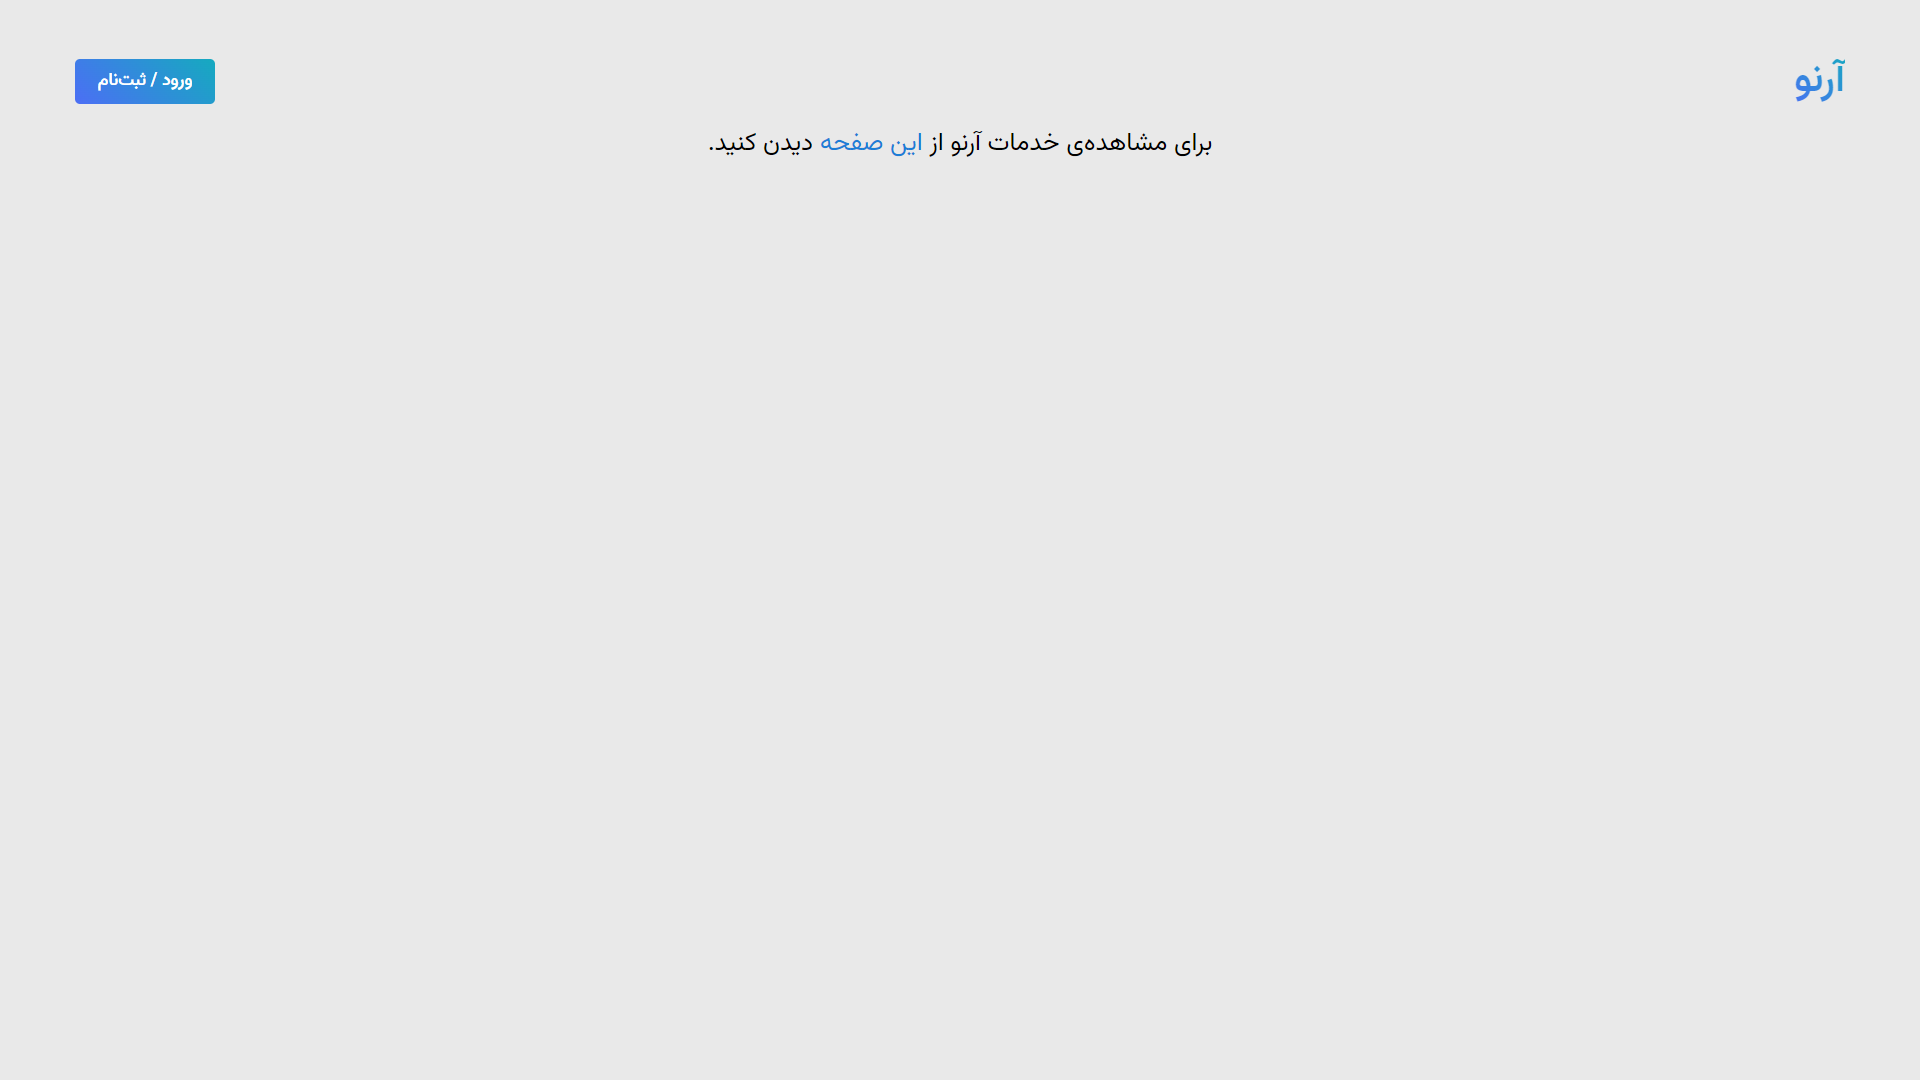
\includegraphics[width=\textwidth]{figs/initial-ui/homepage}
	\caption{صفحه اصلی}
	\label{homepage}
\end{figure}

\subsection{زیرسیستم کاربری}

\subsubsection{‌ثبت‌نام و ویرایش اطلاعات کاربری}
شکل
\ref{req-15}
نمایانگر این ویژگی (شماره 15) است. در شکل
\ref{signup}
فرم ثبت نام و در شکل
\ref{edit-profile}

صفحه ویرایش پروفایل نمایش داده شده است. در این شکل در صورت ورود متخصص امکان فعال/غیرفعال کردن حساب نیز در فرم قرار گرفته است.

\begin{figure*}[h]
	\centering
	\begin{subfigure}[b]{\textwidth}
		\centering
		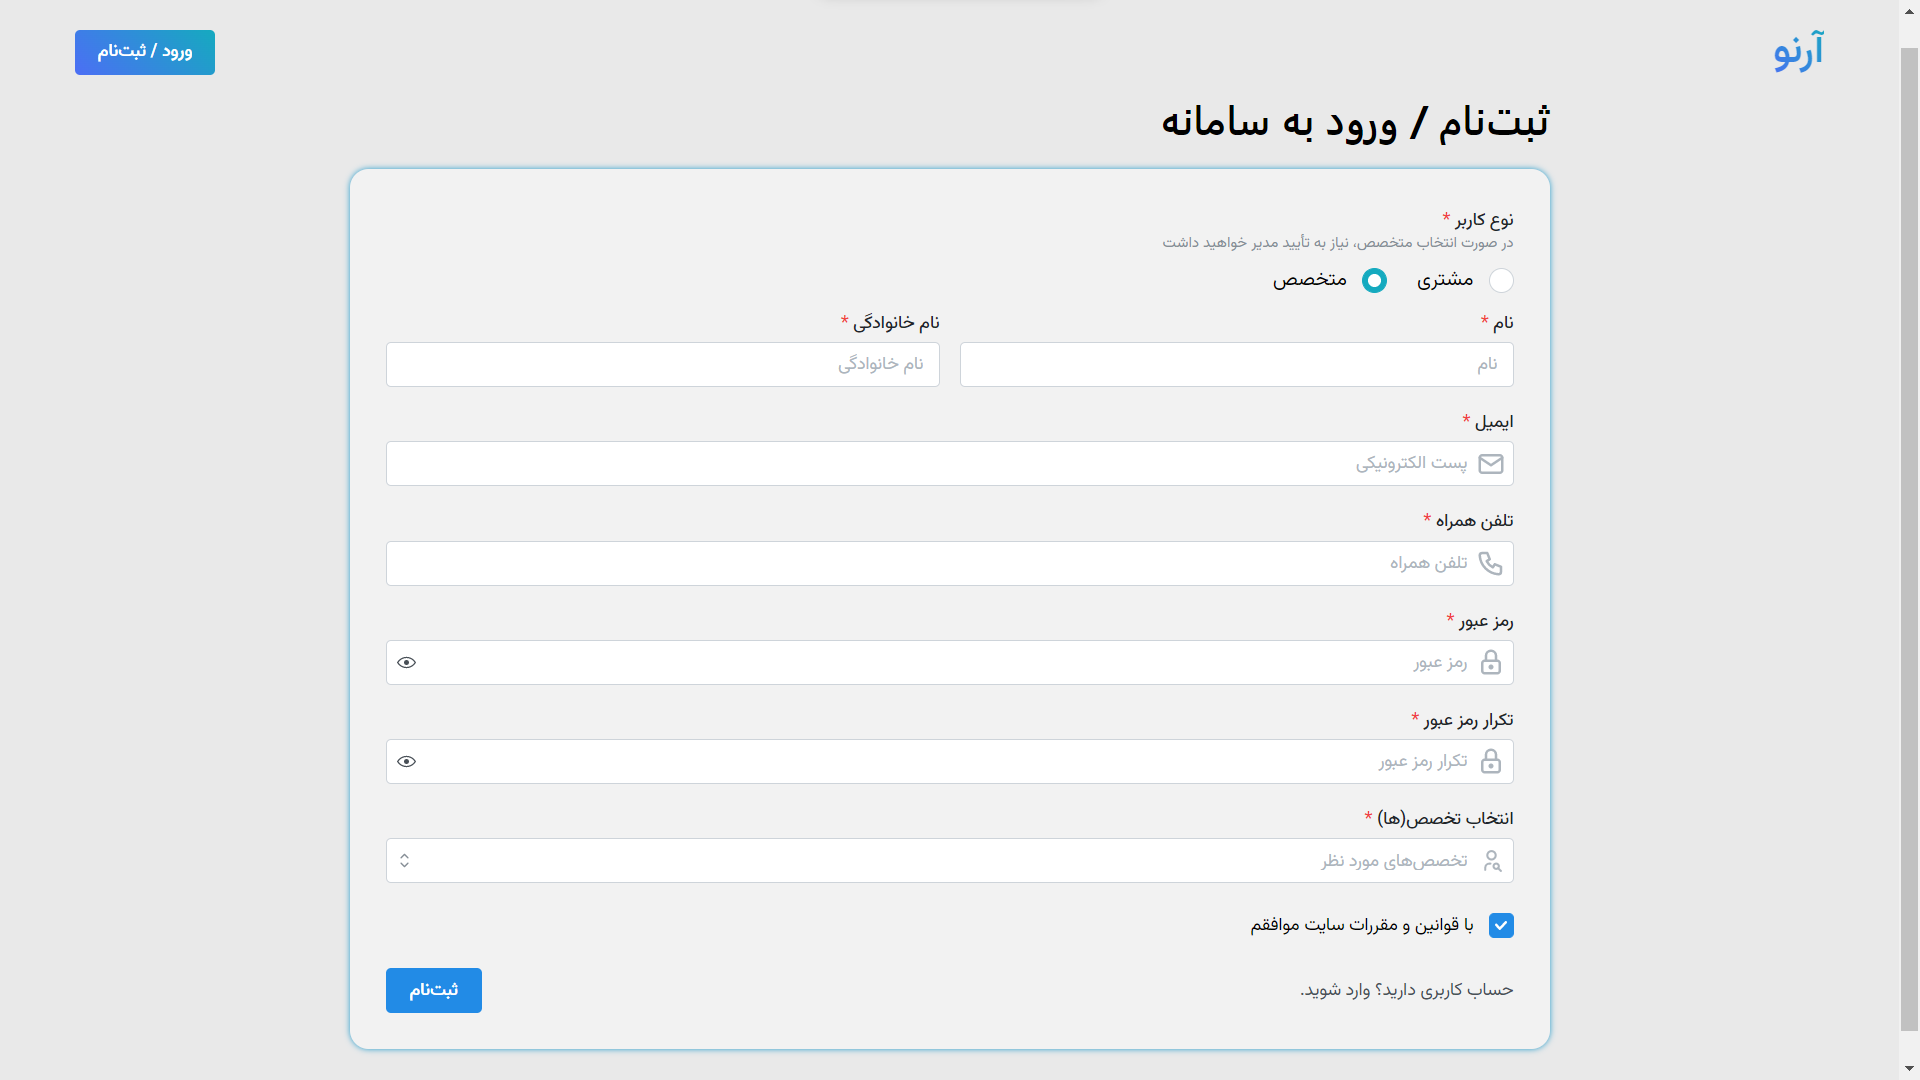
\includegraphics[width=\textwidth]{figs/initial-ui/signup}
		\caption[صفحه ثبت‌نام: در این قسمت در صورت انتخاب «متخصص» فیلد «انتخاب تخصص(ها)» نمایان می‌شود.]%
		{{\small صفحه ثبت‌نام: در این قسمت در صورت انتخاب «متخصص» فیلد «انتخاب تخصص(ها)» نمایان می‌شود.}}    
		\label{signup}
	\end{subfigure}
	\begin{subfigure}[b]{\textwidth}   
		\centering 
		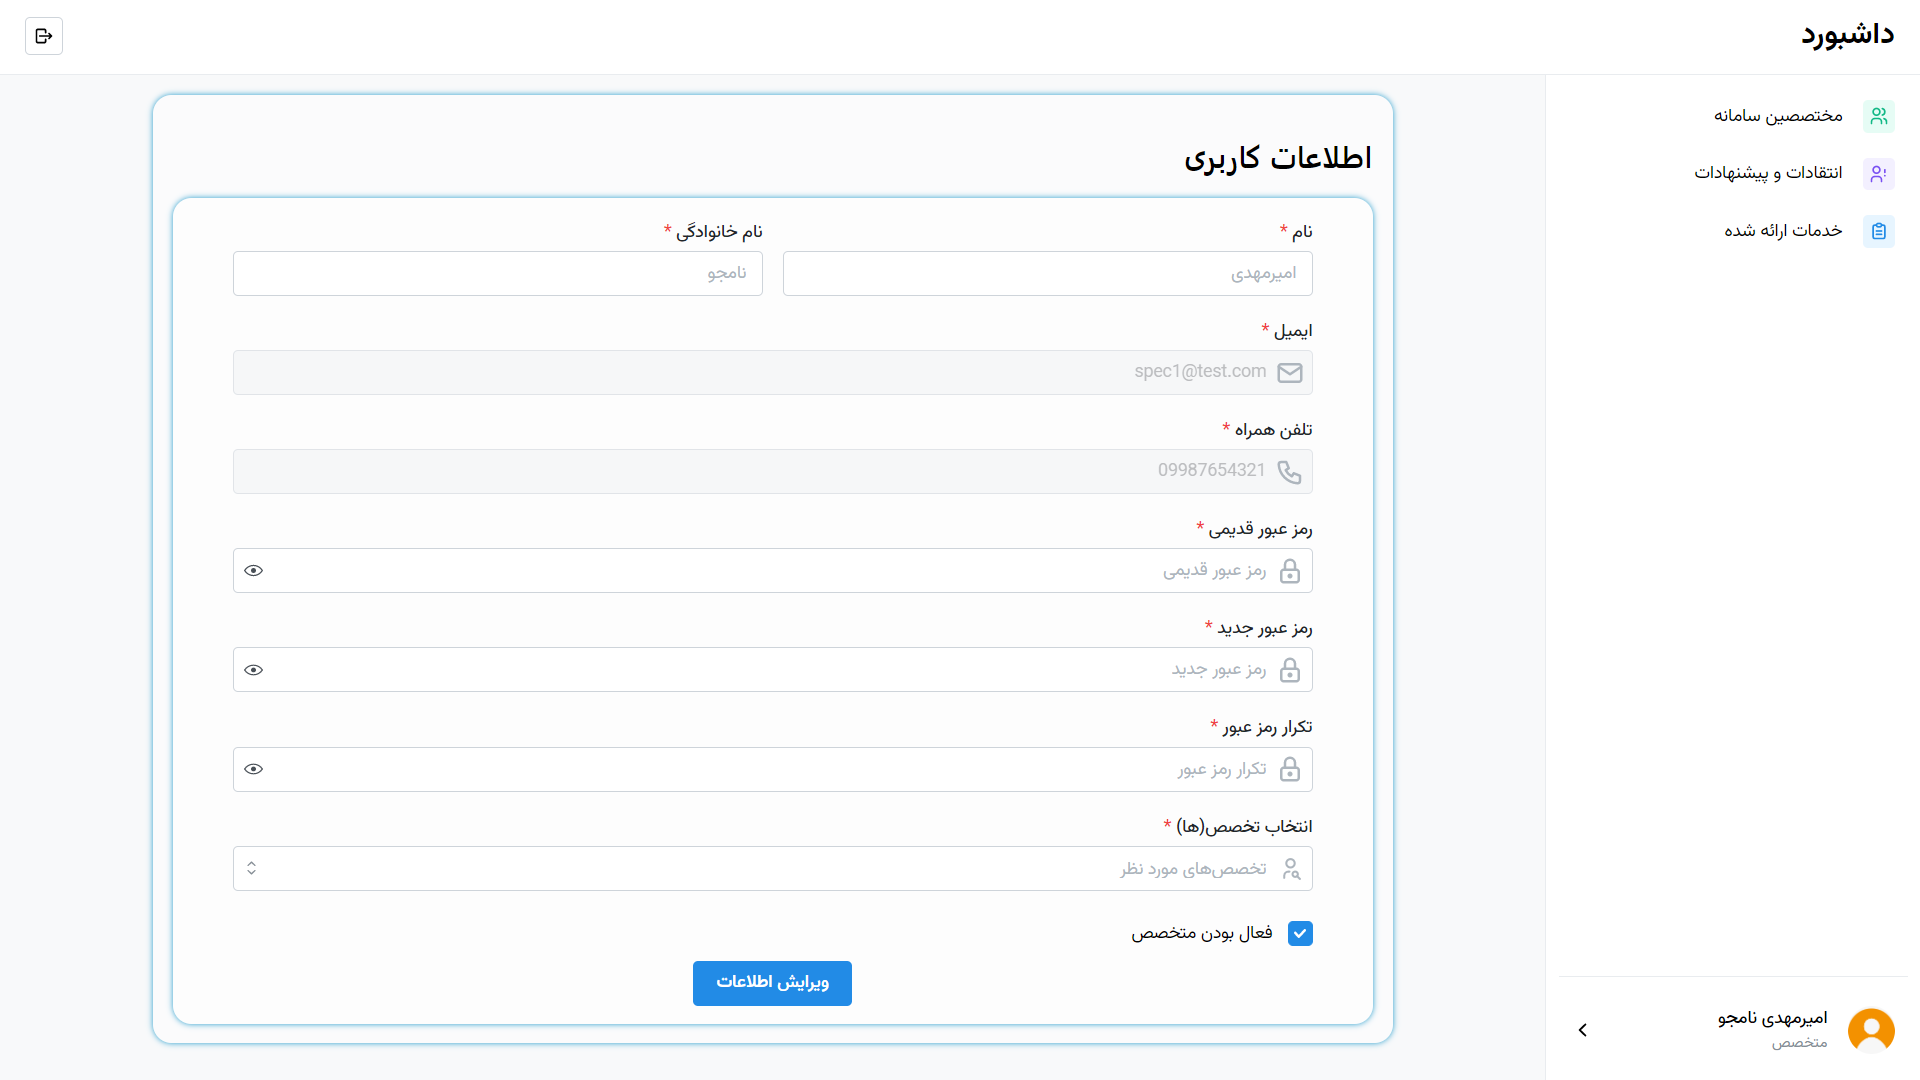
\includegraphics[width=\textwidth]{figs/initial-ui/edit-profile}
		\caption[ویرایش اطلاعات: این صفحه (قابل دسترسی از پایین داشبورد) به کاربران مختلف امکان ویرایش اطلاعات مربوط به نوع کاربری خود را می‌دهد.]%
		{{\small ویرایش اطلاعات: این صفحه (قابل دسترسی از پایین داشبورد) به کاربران مختلف امکان ویرایش اطلاعات مربوط به نوع کاربری خود را می‌دهد.}}    
		\label{edit-profile}
	\end{subfigure}
	\caption[ثبت‌نام و ویرایش پروفایل]
	{\small ثبت‌نام و ویرایش پروفایل} 
	\label{req-15}
\end{figure*}

\subsubsection{مشاهده لیست متخصصین براساس امتیاز}
این ویژگی (شماره 3) در شکل
\ref{spec-specialists}
به تصویر کشیده شده است. همانطور که مشاهده می‌شود متخصصین به‌ترتیب نزولی میانگین امتیاز مرتب شده‌اند.

\begin{figure}[h]
	\centering
	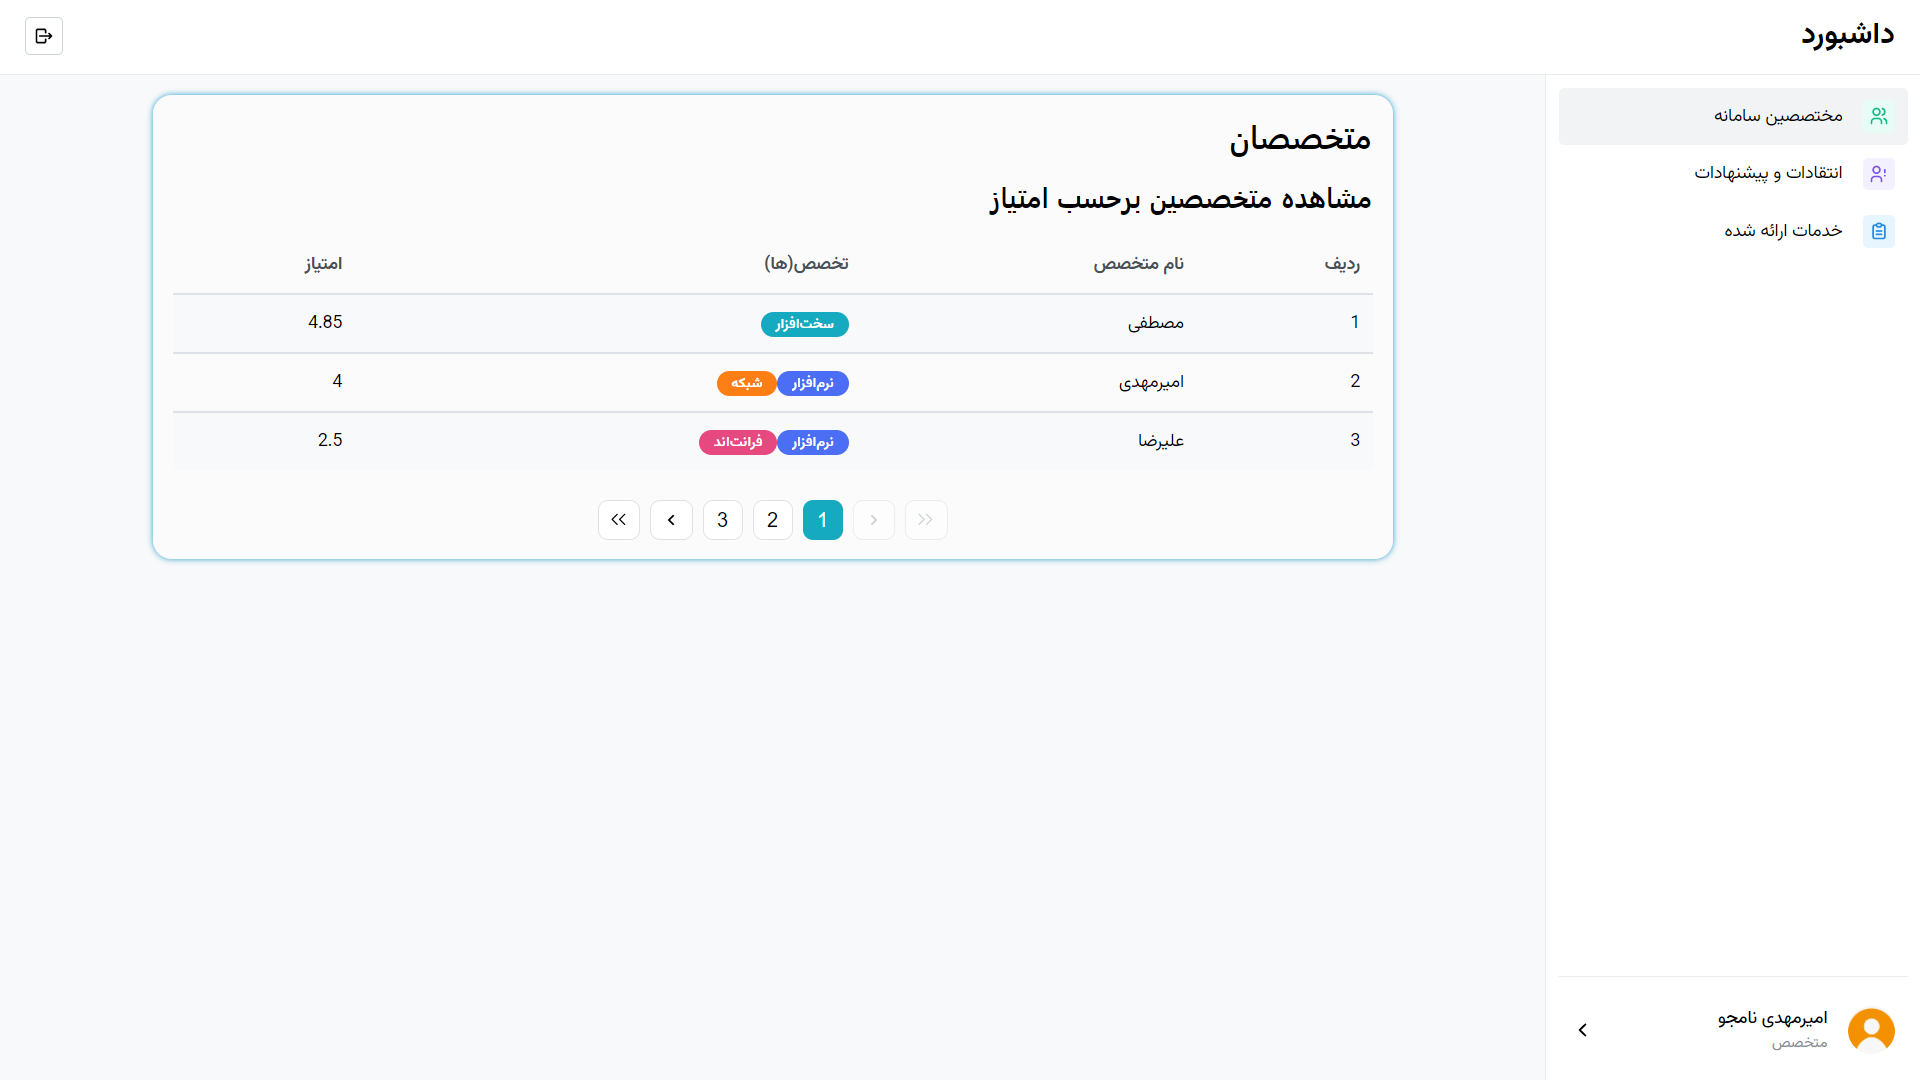
\includegraphics[width=\textwidth]{figs/initial-ui/spec-specialists}
	\caption{مشاهده متخصصین (قابل دسترسی برای همه کاربران)}
	\label{spec-specialists}
\end{figure}

\subsubsection{جست‌وجو در لیست متخصصین}
این ویژگی (شماره 11) در شکل
\ref{ctmr-specialists}
ترسیم شده است. همانطور که مشاهده می‌شود مشتریان می‌توانند علاوه بر مشاهده لیست متخصصین (که در قسمت قبل نشان داده شده) براساس تخصص‌ها و نام متخصص(های) مدنظر خود را بیابند.

\begin{figure}[h]
	\centering
	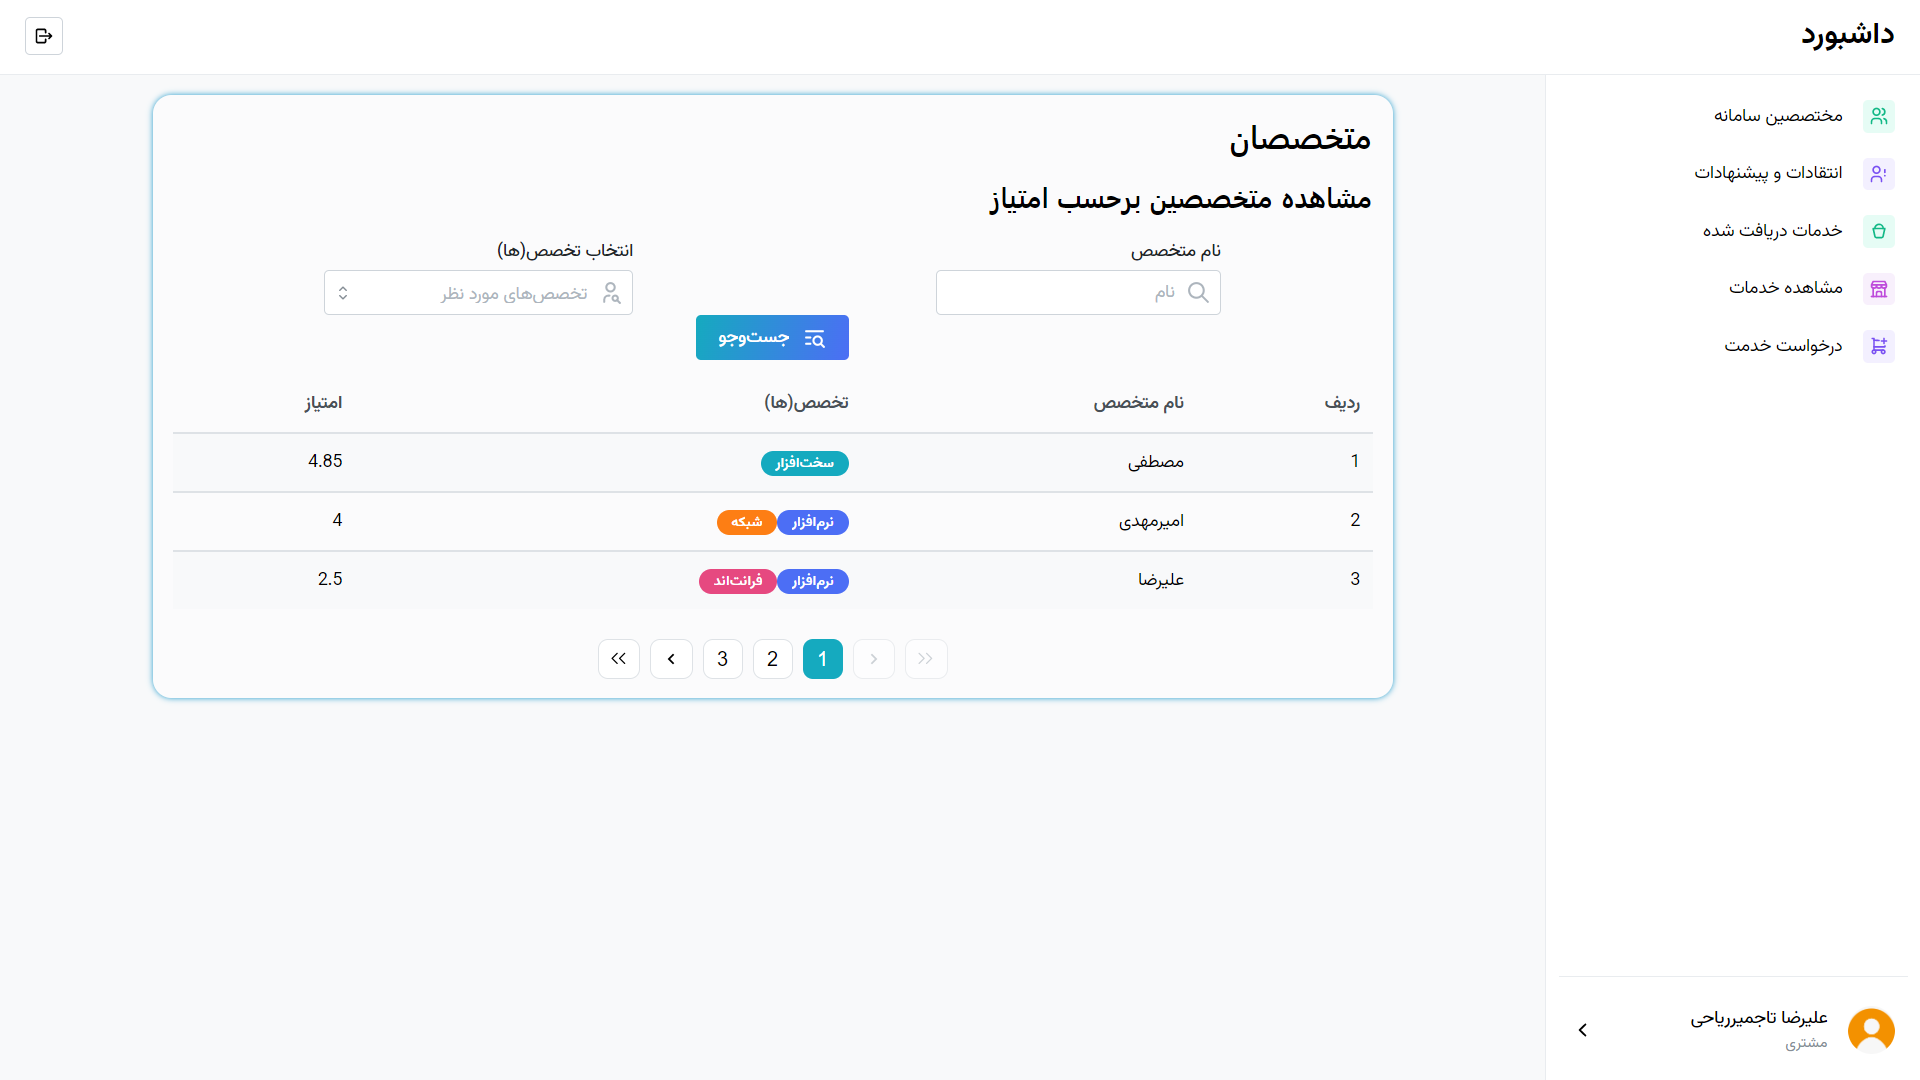
\includegraphics[width=\textwidth]{figs/initial-ui/ctmr-specialists}
	\caption{مشاهده متخصصین (قسمت جست‌وجو فقط برای مشتریان)}
	\label{ctmr-specialists}
\end{figure}


\subsection{زیرسیستم خدمت‌دهی}

\subsubsection{جست‌وجو و مشاهده خدمات}

در شکل
\ref{ctmr-services}
ویژگی جست‌وجو و مشاهده خدمات دسته‌بندی شده (شماره 10) نمایش داده شده است. این قابلیت تنها برای مشتریان وجود دارد.

\begin{figure}[h]
	\centering
	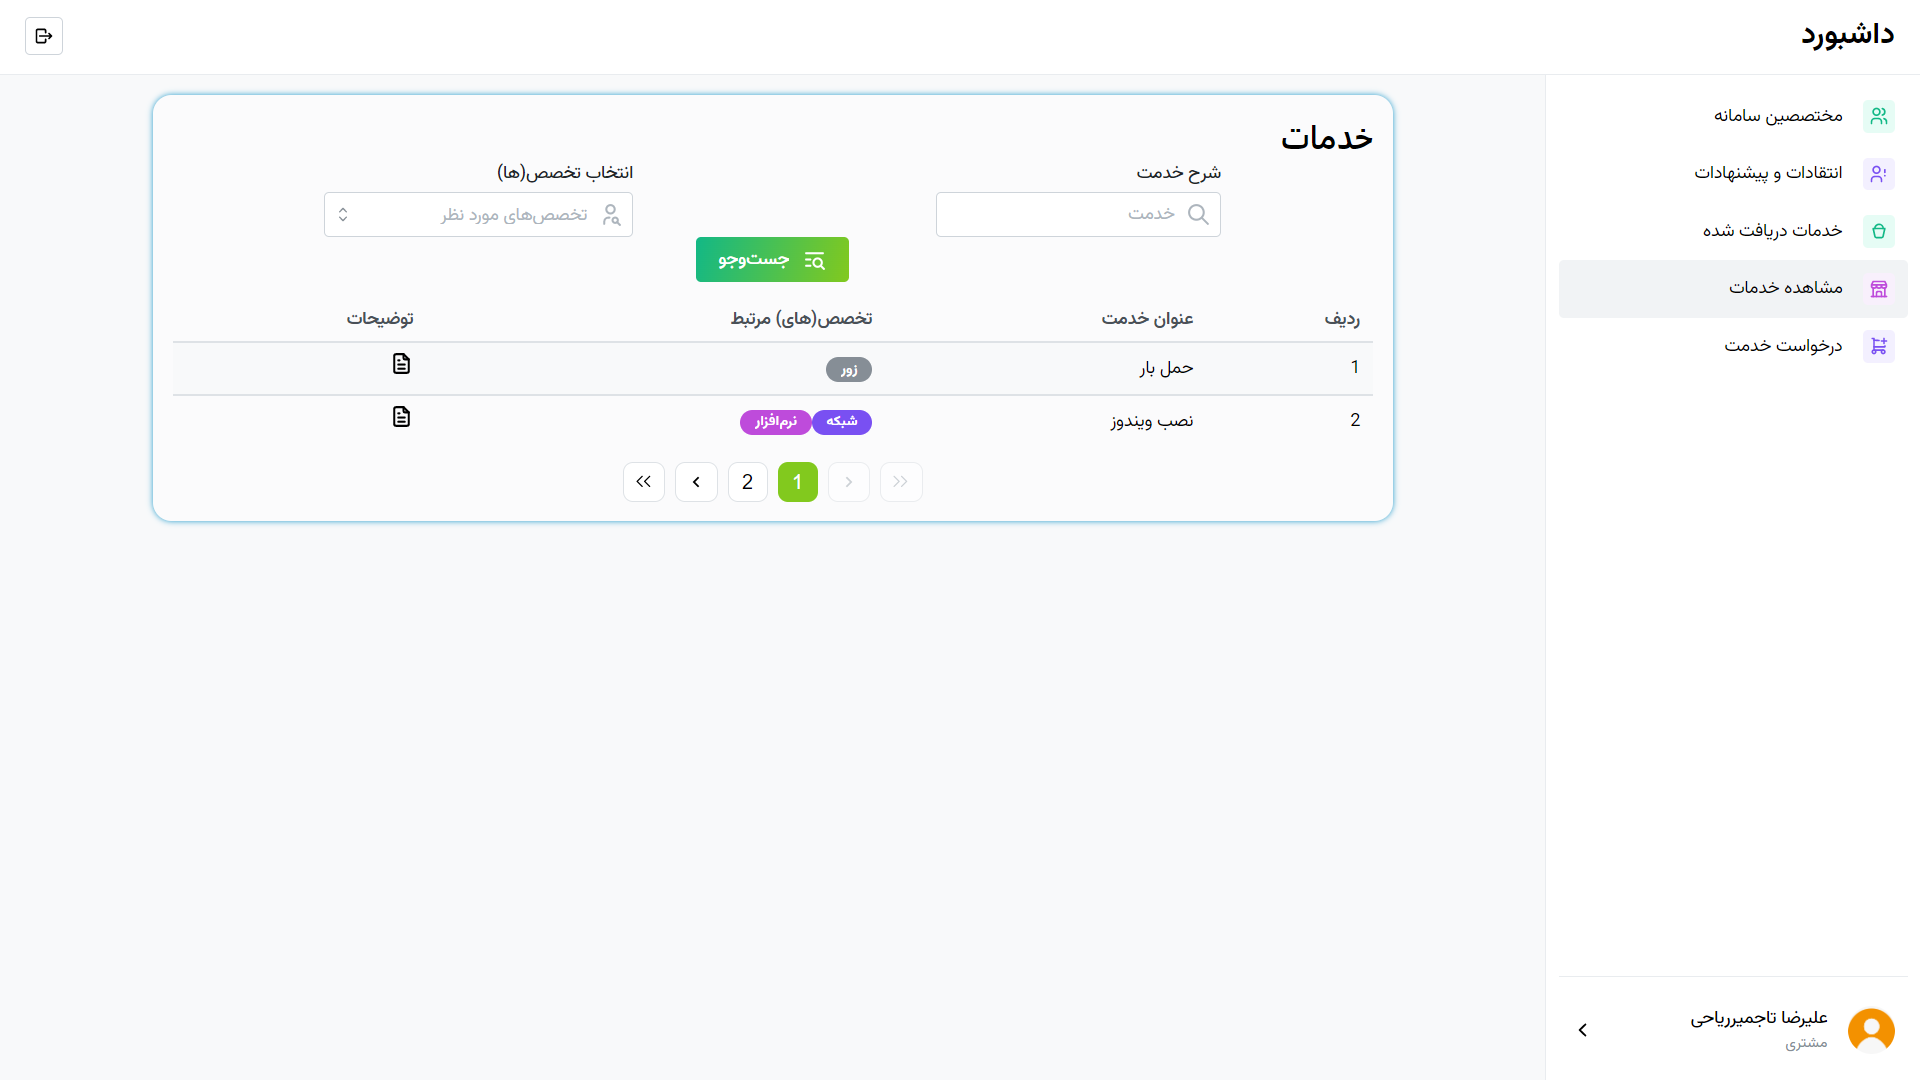
\includegraphics[width=\textwidth]{figs/initial-ui/ctmr-services}
	\caption{مشاهده و جست‌وجو در خدمات}
	\label{ctmr-services}
\end{figure}

\subsubsection{دو ویژگی رد متخصص و مشاهده وضعیت درخواست‌ها}
ویژگی‌های ذکر شده (شماره 12 و 24) در صفحه‌ی «سفارش‌های من» در پنل مشتری قرار گرفته‌اند که در شکل
\ref{ctmr-requests-spec}
نمایش داده شده است.

\begin{figure}[h]
	\centering
	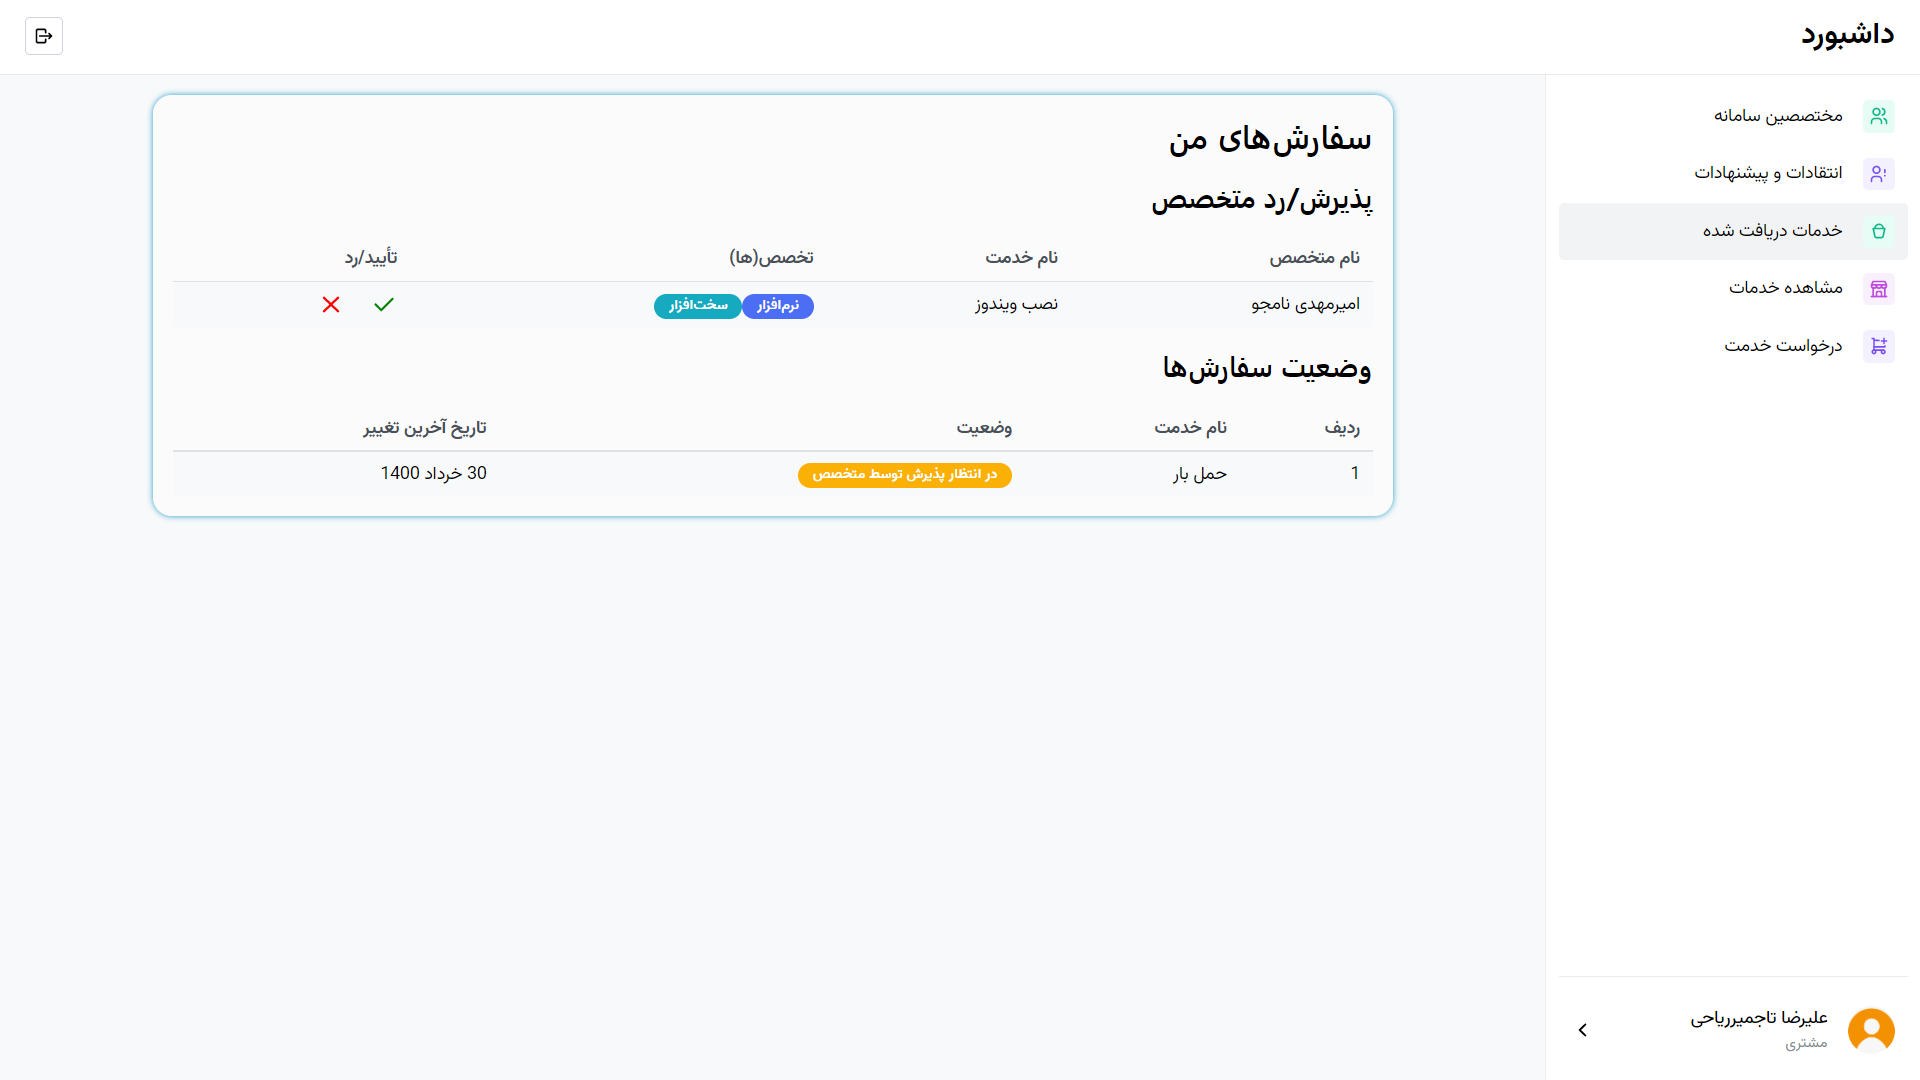
\includegraphics[width=\textwidth]{figs/initial-ui/ctmr-requests-spec}
	\caption{رد متخصص و نمایش وضعیت درخواست‌های مشتری}
	\label{ctmr-requests-spec}
\end{figure}

\subsubsection{دو ویژگی رد درخواست مشتری و دریافت پیام}
ویژگی‌های ذکر شده (شماره 13 و 14) در صفحه‌ی «خدمات ارائه شده» در پنل متخصص در شکل
\ref{spec-request-notif}
نشان داده شده‌اند (اعلان به متخصص در پایین چپ صفحه ظاهر می‌شود).

\begin{figure}[h]
	\centering
	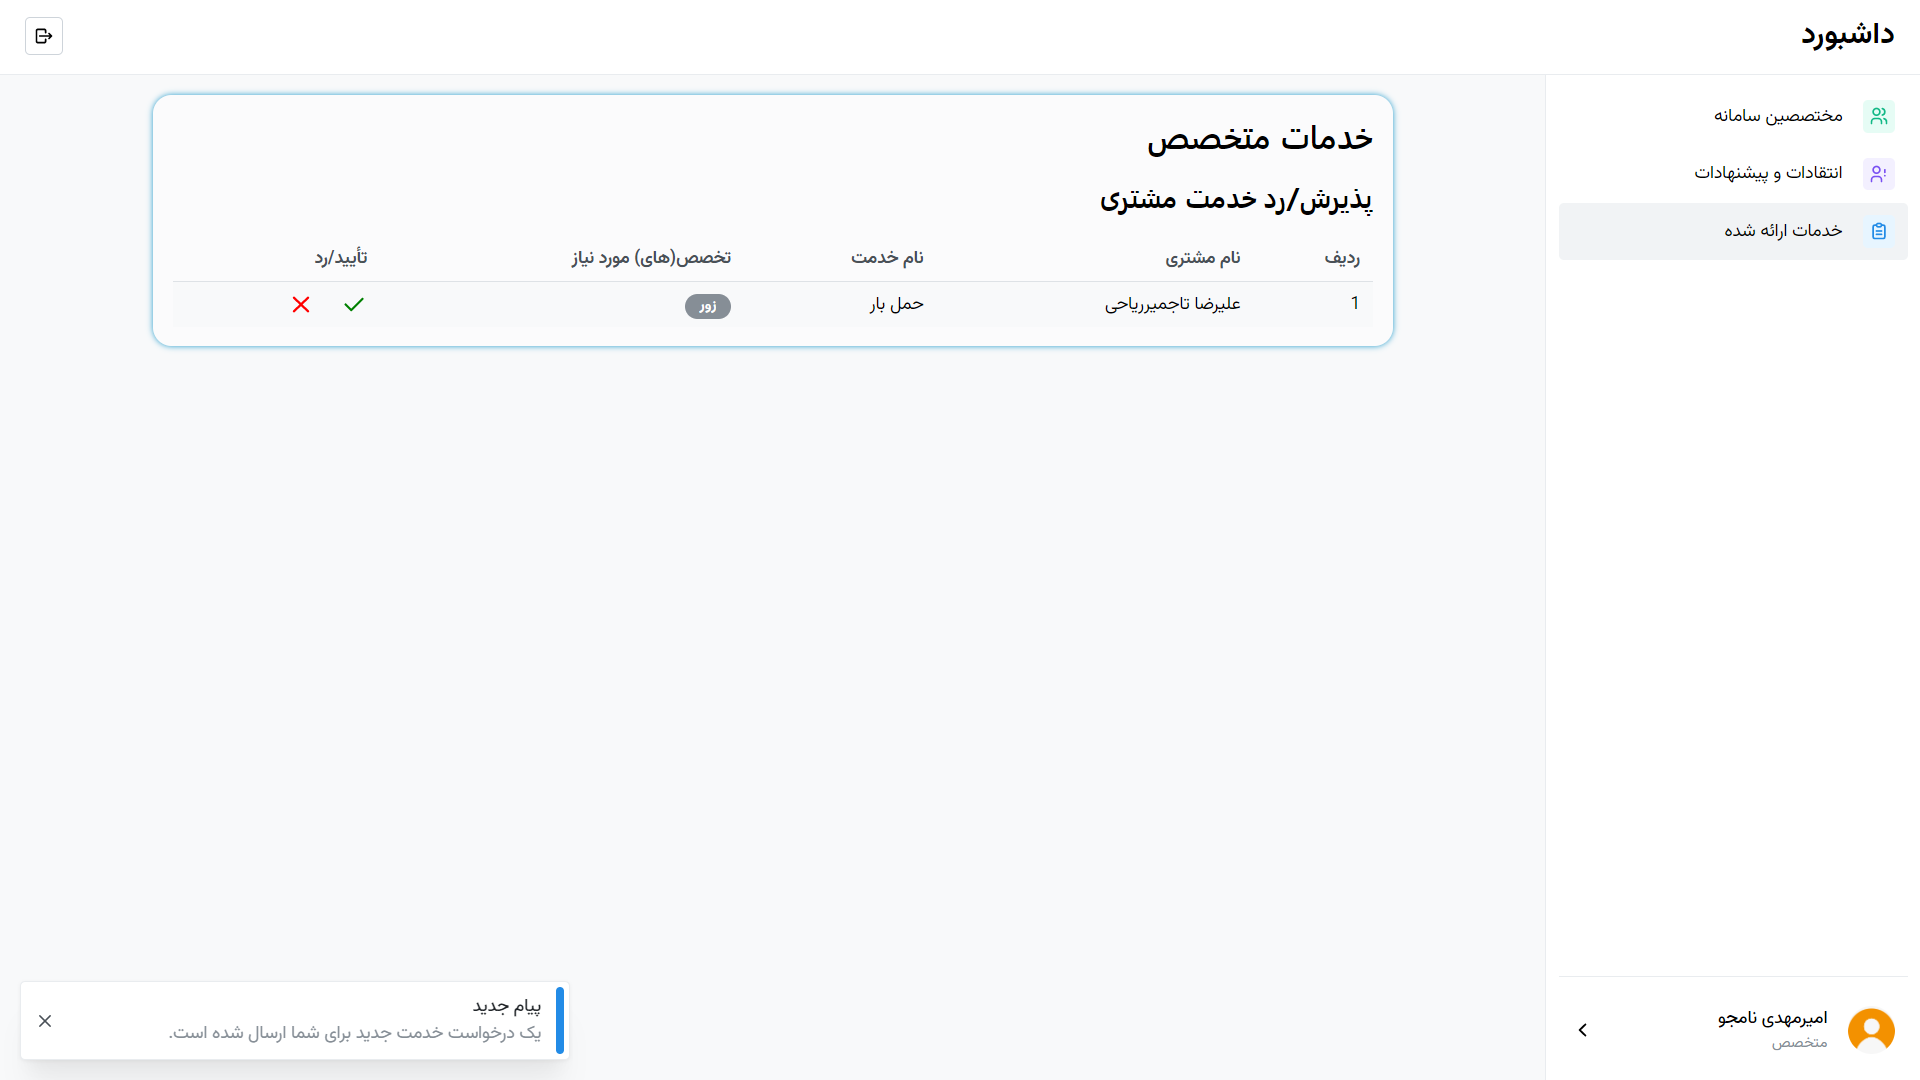
\includegraphics[width=\textwidth]{figs/initial-ui/spec-request-notif}
	\caption{پذیرش/رد مشتری توسط متخصص و دریافت اعلان}
	\label{spec-request-notif}
\end{figure}

\subsection{زیرسیستم گزارش‌گیری}

\subsubsection{دریافت گزارش مشکلات فنی}
شکل
\ref{mngr-tech-report}
ویژگی شماره 1 یعنی دریافت گزارش مشکلات فنی توسط مدیران را نشان می‌دهد. همچنین در شکل امکان مشاهده پاسخ مدیر فنی برای مدیر شرکت (ویژگی شماره 2) هم وجود دارد که در بخش مربوطه به آن پرداخته شده است.

\begin{figure}[h]
	\centering
	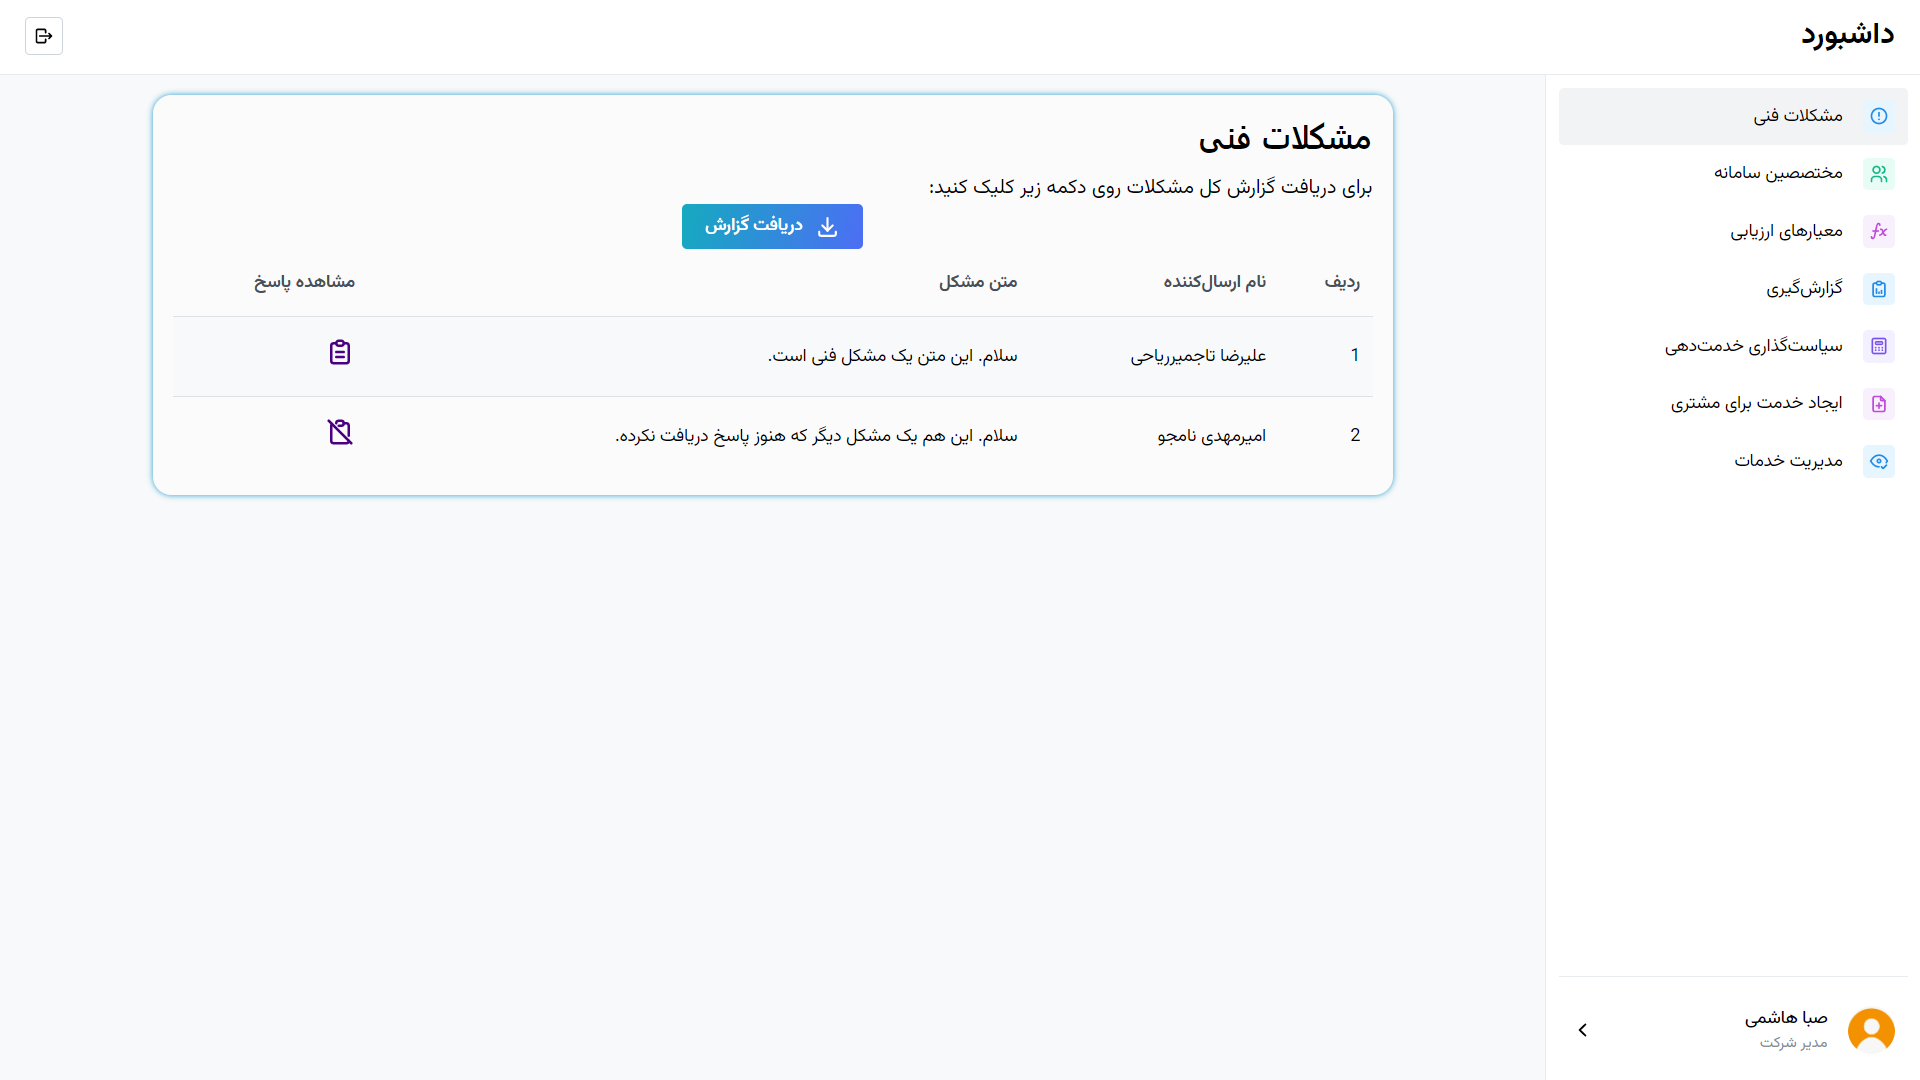
\includegraphics[width=\textwidth]{figs/initial-ui/mngr-tech-report}
	\caption{مشکلات فنی در پنل مدیر شرکت}
	\label{mngr-tech-report}
\end{figure}


\subsubsection{ارسال پاسخ به مشکلات فنی}
شکل
\ref{tech-tech-report}
ویژگی شماره 2 را نشان می‌دهد که طی آن مدیر فنی امکان مشاهده و ارسال پاسخ به مشکلات فنی کاربران را (با کلیک روی ستون سمت چپ جدول و نوشتن متن در یک \lr{Modal}) دارد. همانطور که در شکل
\ref{mngr-tech-report}
نشان داده شد، مدیر امکان مشاهده این پاسخ را خواهد داشت.

\begin{figure}[h]
	\centering
	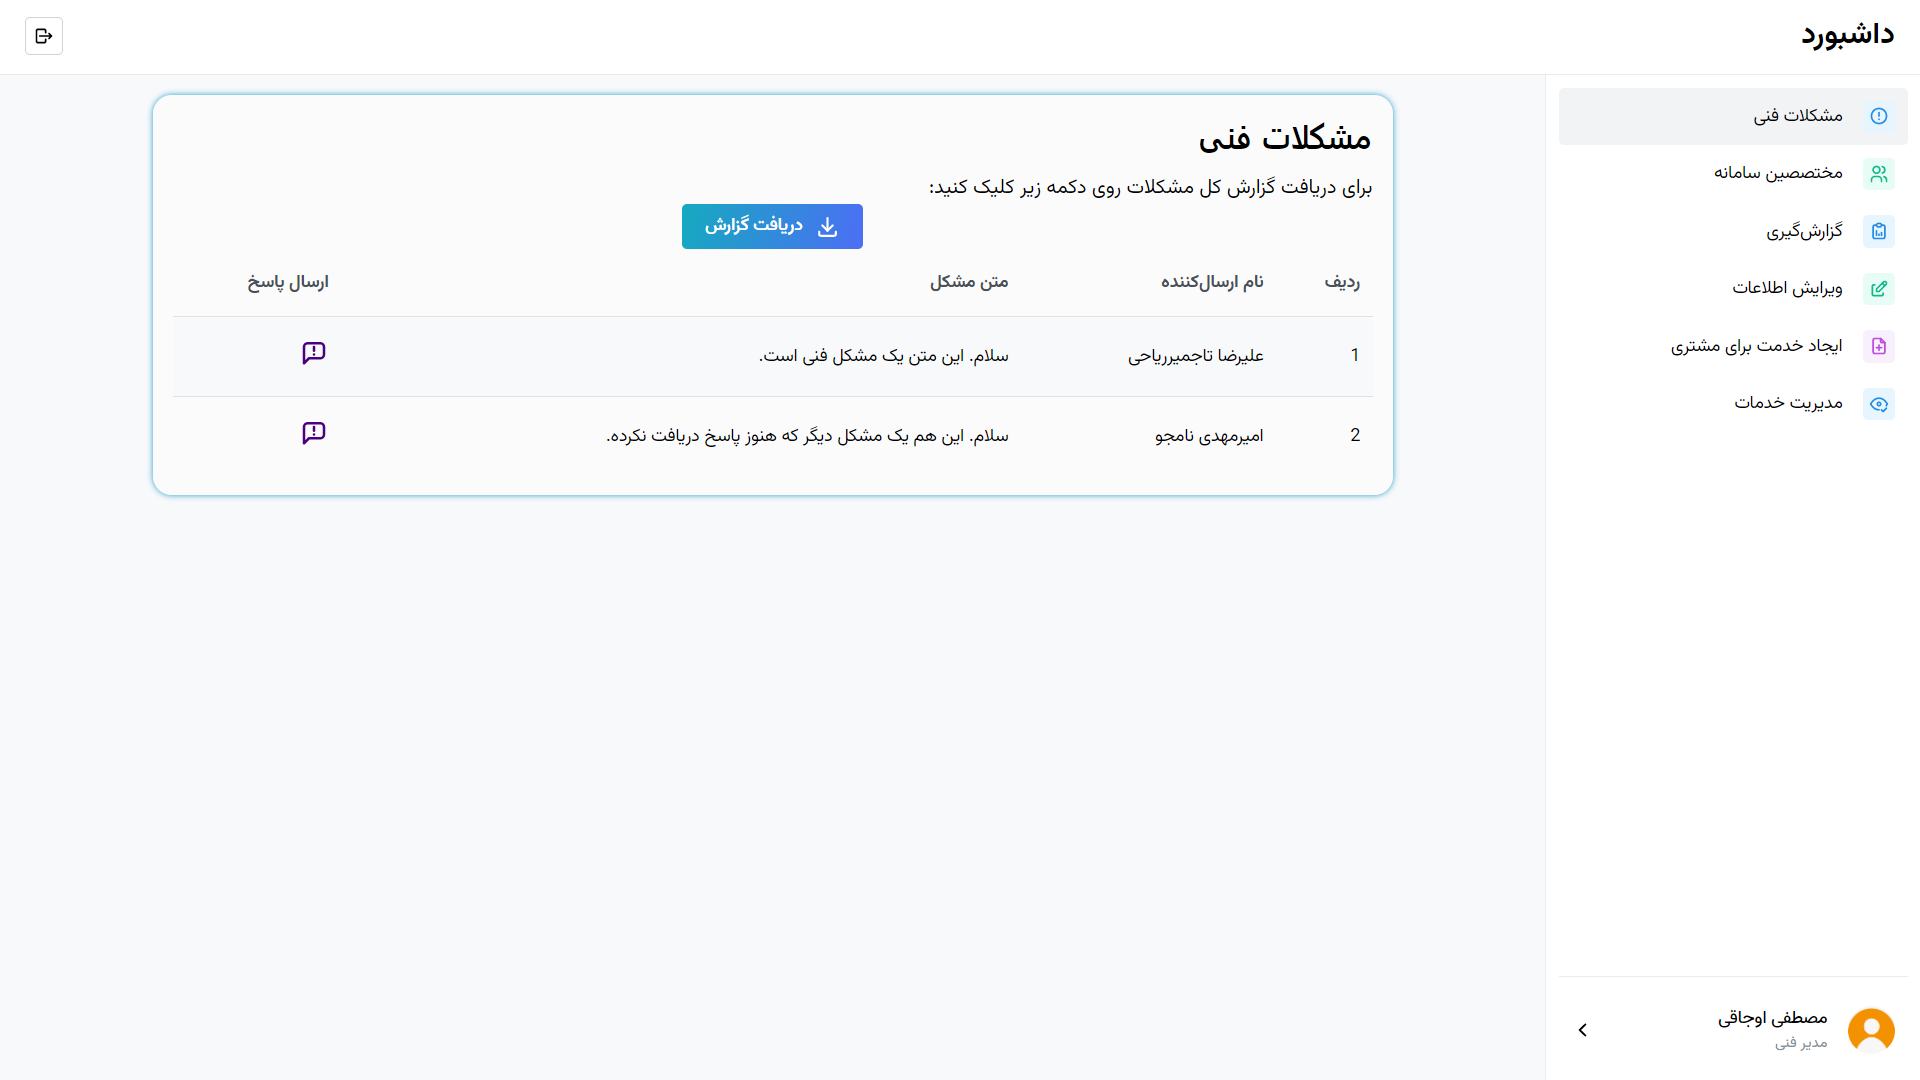
\includegraphics[width=\textwidth]{figs/initial-ui/tech-tech-report}
	\caption{مشکلات فنی در پنل مدیر فنی}
	\label{tech-tech-report}
\end{figure}

\subsection{زیرسیستم بازخورد}

\subsubsection{ثبت انتقادات، پیشنهادات و مشکلات فنی}
این ویژگی (شماره 5) در داشبورد متخصصین و مشتریان مطابق شکل
\ref{suggestions}
قرار گرفته و امکان ارسال انتقادات، پیشنهادات و مشکلات فنی را با ذکر نوع پیام فراهم می‌کند.

\begin{figure}[h]
	\centering
	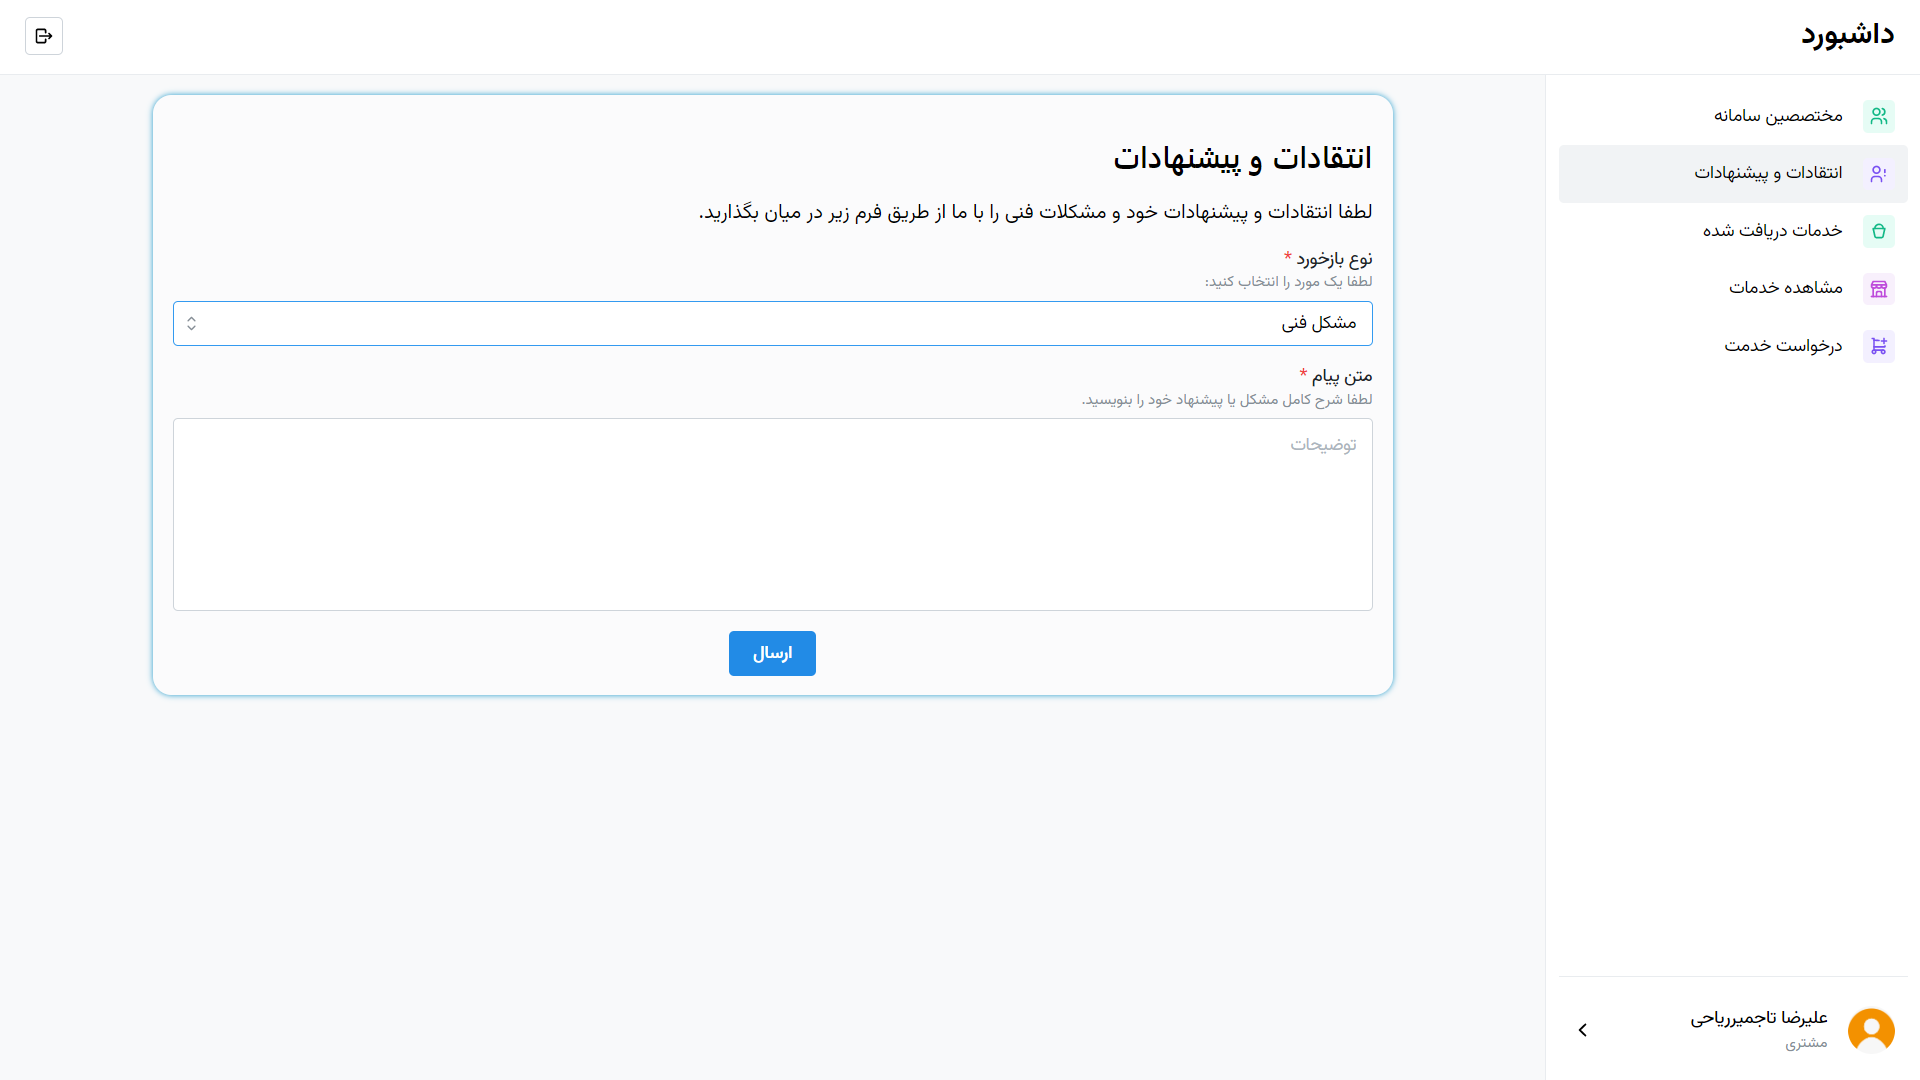
\includegraphics[width=\textwidth]{figs/initial-ui/suggestions}
	\caption{انتقادات، پیشنهادات و مشکلات فنی}
	\label{suggestions}
\end{figure}

\subsection{زیرسیستم مدیریت}

\subsubsection{تعیین سقف تعداد خدمات بر اساس امتیاز}
این ویژگی (شماره 9) که برای مدیر شرکت فراهم است در تصویر
\ref{policy}
نمایش داده شده است.

\begin{figure}[h]
	\centering
	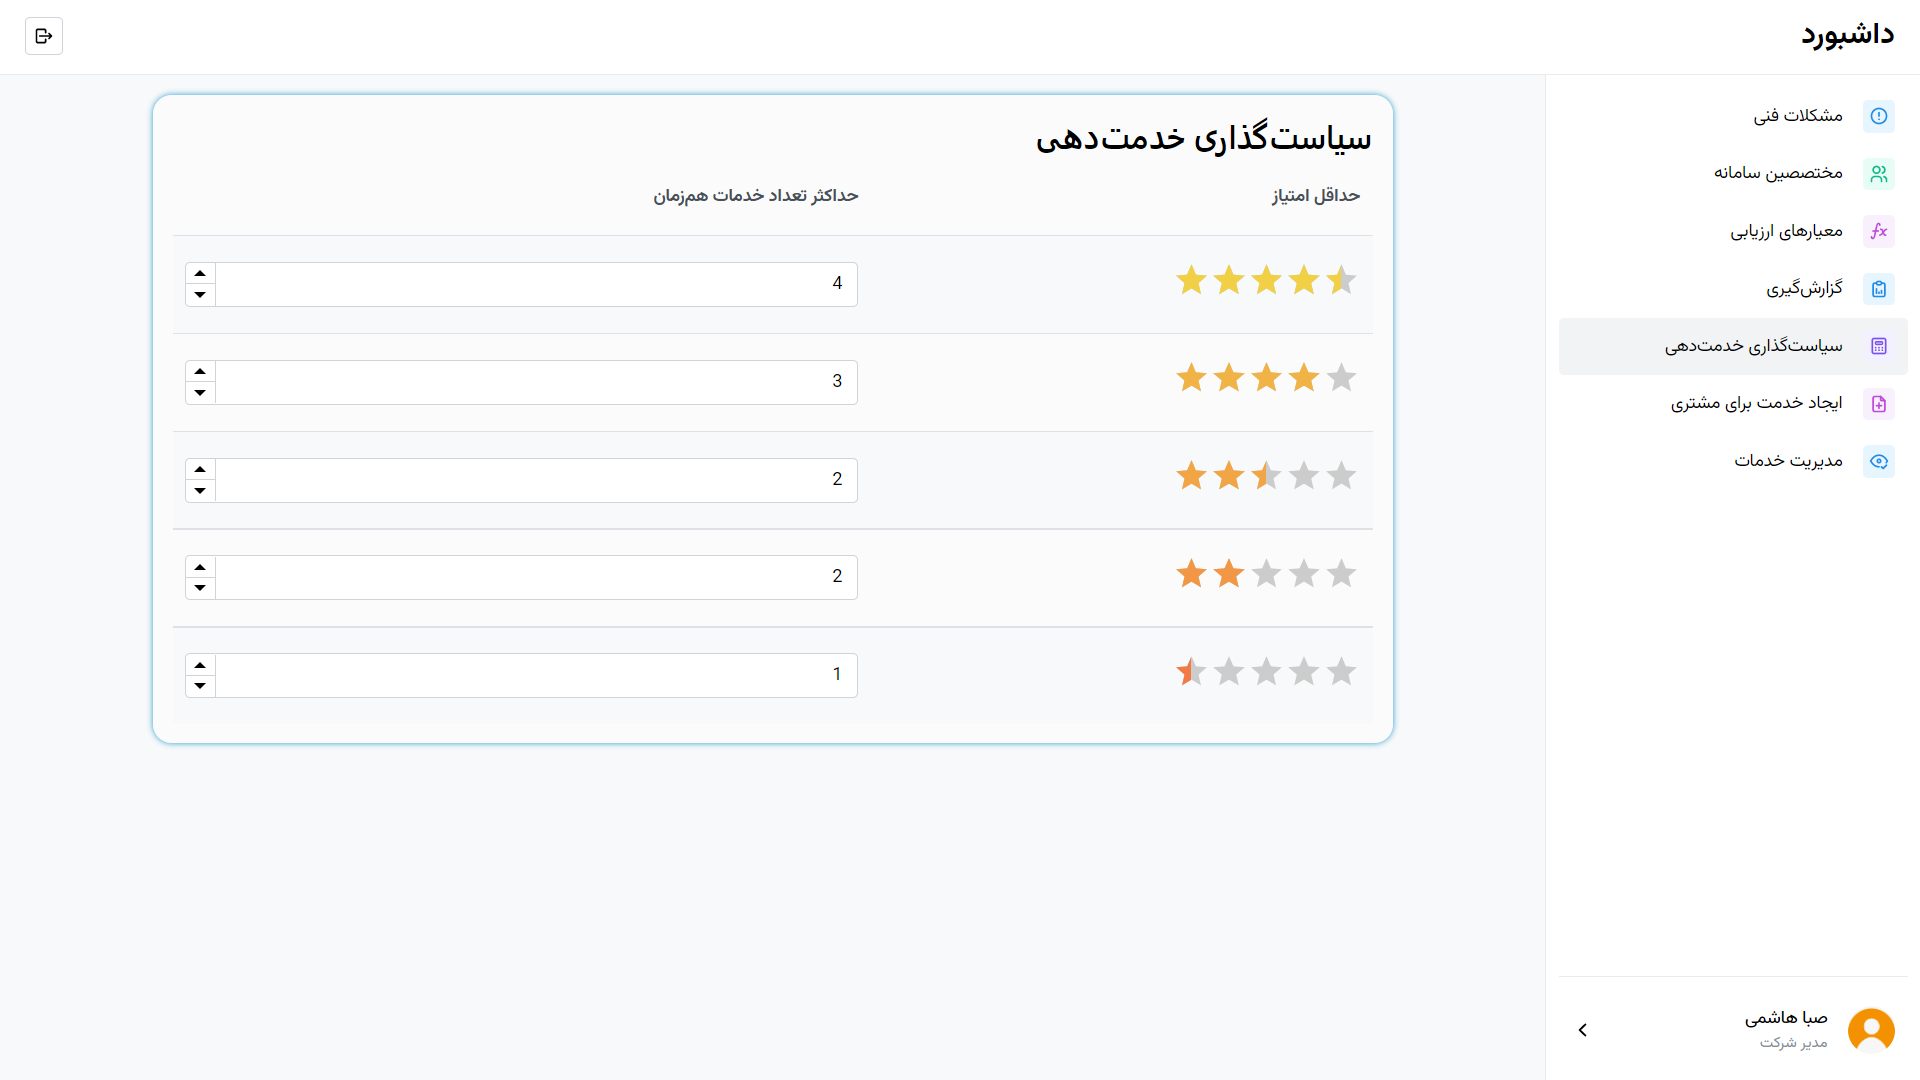
\includegraphics[width=\textwidth]{figs/initial-ui/service-policy}
	\caption{سیاست‌گذاری سقف تعداد خدمات متخصصین}
	\label{policy}
\end{figure}


\subsubsection{امکان تأیید متخصصین}
این ویژگی (شماره 18) در بالای شکل
\ref{mngr-specialists}
نشان داده شده است. قسمت دوم این شکل همان ویژگی شماره 3 (مشاهده لیست براساس امتیاز) را نشان می‌دهد که در شکل
\ref{ctmr-specialists}
بالاتر برای نوع کاربر غیر مدیر معرفی کردیم.

\begin{figure}[h]
	\centering
	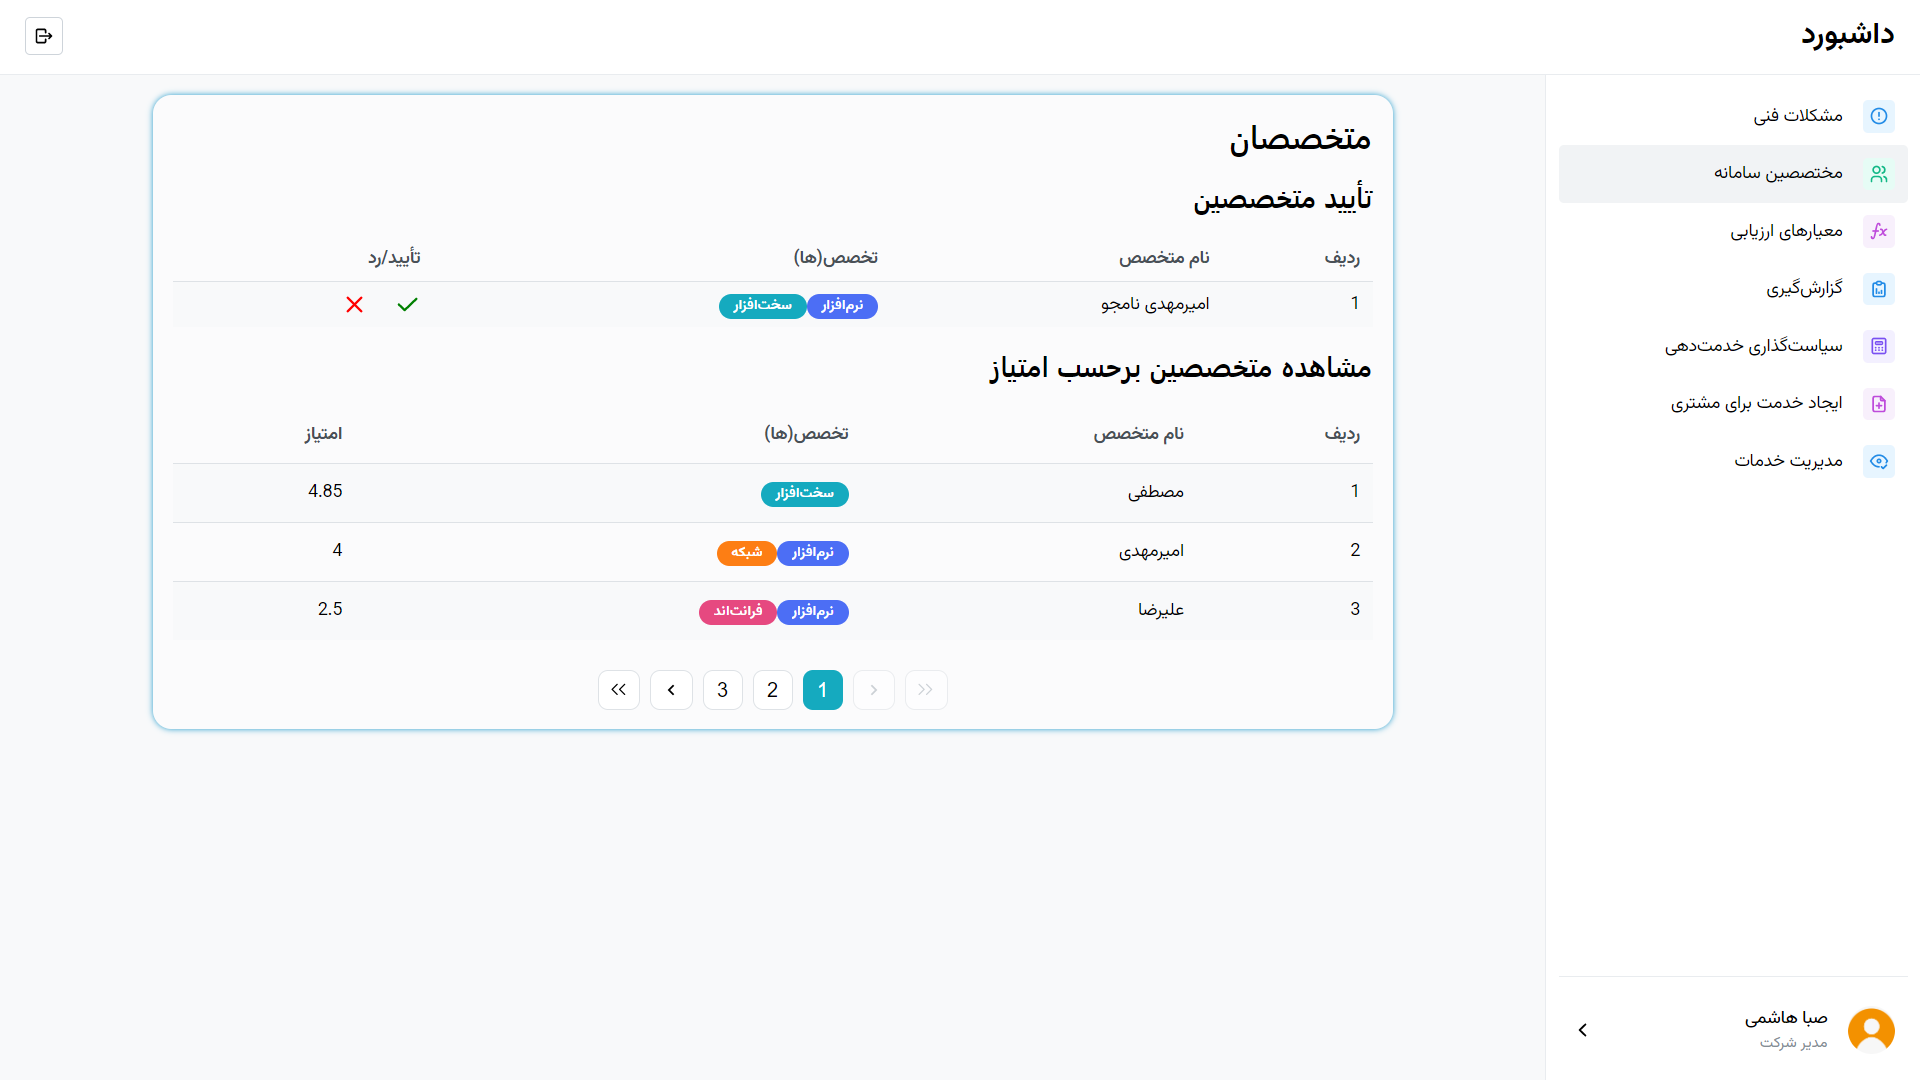
\includegraphics[width=\textwidth]{figs/initial-ui/mngr-specialists}
	\caption{امکان تأیید یا رد متخصص توسط مدیر فنی و مدیر شرکت}
	\label{mngr-specialists}
\end{figure}

\subsubsection{امکان لغو خدمت در هر مرحله}
این ویژگی (شماره 23) به مدیر فنی و مدیر شرکت این اجازه را می‌دهد که خدمات درخواست‌شده‌ی مشتریان را در هر مرحله‌ای لغو کنند. این ویژگی در شکل
\ref{cancel-service}
نمایش داده شده است.

\begin{figure}[h]
	\centering
	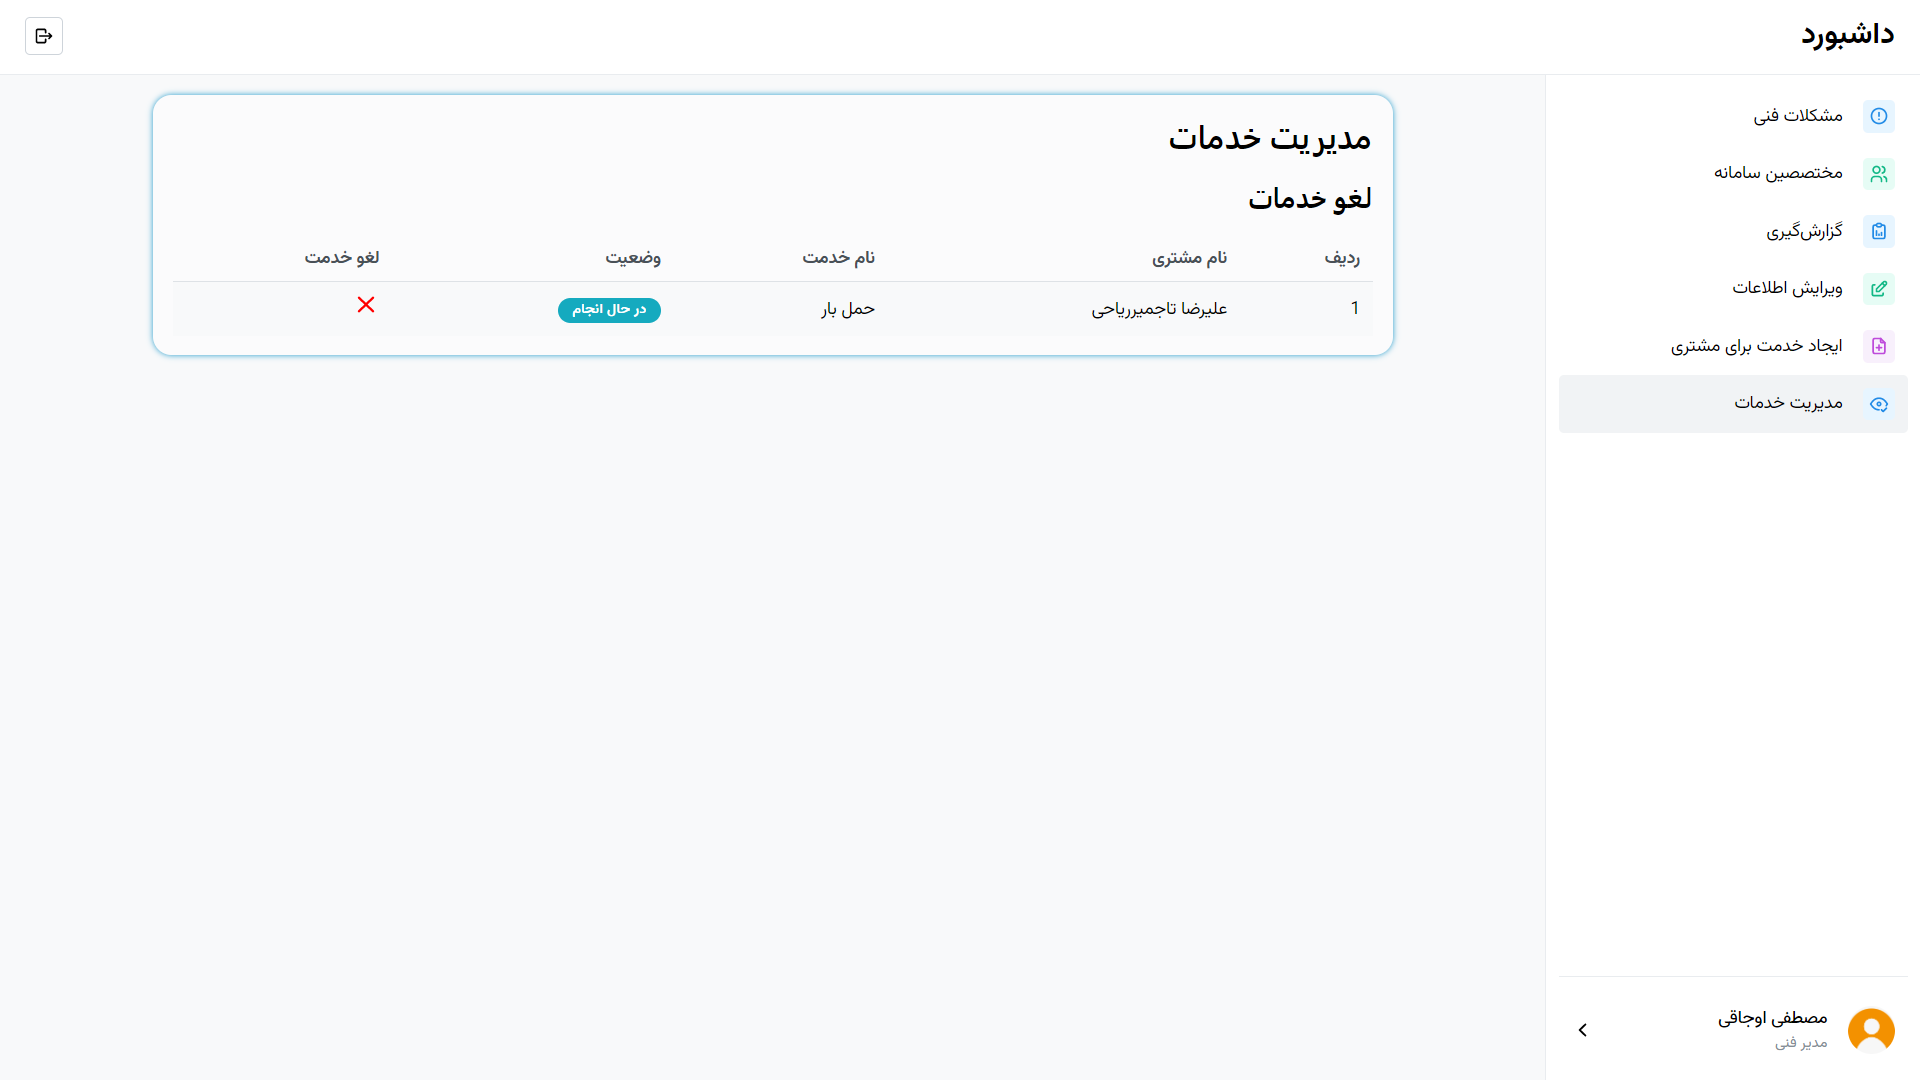
\includegraphics[width=\textwidth]{figs/initial-ui/cancel-service}
	\caption{امکان تأیید یا رد متخصص توسط مدیر فنی و مدیر شرکت}
	\label{cancel-service}
\end{figure}










	
\chapter{ریسک‌ها}

ریسک و مخاطرات، جزئی جدایی ناپذیر و ذاتی از فعالیت‌های تولید نرم‌افزار هستند و از سویی ریسک‌پذیری برای برای پیشرفت ضروری است. تیم تولید یک نرم‌افزار باید بداند که ریسک نه بد است و نه خوب، اما همیشه در پروژه وجود دارد و برخورد مناسب با آن باعث می‌شود که احتمال موفقیت پروژه افزایش یابد.


تمامی پارادایم‌های مدیریت ریسک، شامل فعالیت‌های زیر هستند:

\begin{itemize}
	\item
	 \textbf{شناسایی}:
 پیش از مدیریت ریسک‌ها، باید آن‌ها را شناسایی کرد. شناسایی باعث می‌شود که ریسک‌ها قبل از آن‌ که تبدیل به مشکل بشوند، آشکار بشوند. 
	 
	 \item
	 \textbf{تحلیل}:
 تحلیل یعنی داده‌هایی که از ریسک داریم را به اطلاعاتی که می‌تواند در تصمیم‌گیری مفید واقع شود تبدیل کنیم. این مرحله، به مدیر پروژه کمک می‌کند ریسک‌های پراهمیت را شناسایی کند و در ادامه‌ی فعالیت‌ها، وقت بیشتری برای کنترل این ریسک‌ها بگذارد.
	 
	 \item 
	 \textbf{برنامه‌ریزی}:
 در مرحله برنامه‌ریزی، با توجه به اطلاعاتی که از ریسک وجود دارد تصمیماتی برای اقدامات بعدی گرفته می‌شود. بسته به نوع ریسک، برنامه‌های مختلفی نظیر کاهش اثر ریسک، پرهیز از ریسک، پذیرش ریسک، مطالعه بیش‌تر ریسک و غیره را می‌توان ترتیب داد.
	 
	 \item
	\textbf{پیگیری کردن}:
پیگیری کردن به معنی این است که وضعیت ریسک‌ها و اعمالی که برای مقابله با آنان پیش‌بینی شده، به طور دائمی نظارت شوند تا از درستی روند کاهش اثر ریسک اطمینان حاصل شود.
	 
	 \item 
	\textbf{کنترل}:
 کنترل ریسک به معنی اصلاح انحراف‌هایی است که از برنامه تنظیم شده برای مقابله با ریسک ایجاد شده‌اند.
	 
	 \item
	\textbf{ارتباطات}:
 ارتباط برقرار کردن با اعضای تیم در مورد ریسک، در هسته مدل‌های مدیریت ریسک قرار دارد. بدون ارتباطات موثر هیچ پاردایم مدیریت ریسکی قابل اجرا نخواهد بود.
	 
\end{itemize}


با توجه به موارد گفته شده در بالا، در ادامه این مستند به شناسایی ریسک‌هایی که ممکن است پروژه را تحت تاثیر قرار دهد و همچنین در مواردی که ممکن بوده، بعضی از راه‌حل‌های احتمالی آن می‌پردازیم. پیش از بررسی ریسک‌ها باید بدانیم که ریسک‌های تولید نرم‌افزار را می‌توان در سه دسته کلی زیر تقسیم‌بندی کرد:

\begin{itemize}
	\item
	\textbf{مهندسی محصول}:
	 شامل ابعاد فنی کاری که قرار است انجام بشود.
	
	\item
	\textbf{محیط ایجاد}:
	 شامل روش‌ها، فرآیندها و ابزارهایی که برای تولید محصول استفاده می‌شوند.
	
	\item
	\textbf{محدودیت‌های برنامه}:
	 شامل محدودیت‌های سازمانی، قراردادی و عملیاتی که معمولا خارج از کنترل مدیران محلی سیستم است.
\end{itemize}

\section{فهرست ریسک‌ها}

\subsection{ریسک‌های حوزه مهندسی محصول}

ریسک‌های حوزه مهندسی محصول را می‌توان در پنج دسته کلی تقسیم‌بندی کرد. در ادامه به بررسی ریسک‌هایی از هر کدام از دسته‌ها می‌پردازیم.


\subsubsection{نیازمندی‌ها}

\begin{itemize}
	
	\item
	\textbf{پایدار نبودن و امکان تغییر نیازمندی‌ها}
	
	
	توضیح \hspace*{1cm}  پایداری نیازمندی‌ها، به این درجه تغییرات آن‌ها و تاثیراتی است که تغییرات آن‌ها بر کیفیت، برنامه‌زمانی، طراحی، تولید و تست برنامه وارد می‌کند. با توجه به مختصر بودن پروپوزال پروژه و همچنین عدم شناخت جامع تیم بر حوزه پروژه،‌ امکان تغییر در نیازمندی‌ها وجود دارد.
	
	
	راه‌حل \hspace*{1cm}  راه‌حلی که برای این موضوع می‌توان در نظر گرفت، در ابتدا افزایش دانش تیم بر روی موضوع کلی پروژه است تا به مرور پایداری نیاز‌مندی‌ها افزایش یابد. هم با تعامل بیش‌تر با مشتری (دستیاران آموزشی)، نیازمندی‌های اساسی‌تر به طور دقیق‌تر مشخص شوند تا احتمال تغییرات ناگهانی آنان کم شود.
	
	\item 
\textbf{کامل نبودن نیازمندی‌ها}
	
	توضیح \hspace*{1cm}  
	کامل نبودن نیازمندی‌ها،  می‌تواند به دلایلی نظیر عدم شناخت تیم، نبود وقت‌ کافی برای شناسایی دقیق نیازمندی‌ها و یا عدم تعامل مناسب با مشتری ایجاد بشود. البته طبیعتا هیچ‌ وقت نیازمندی‌ها در همان ابتدای کار به طور کامل مشخص نمی‌شوند ولی باید تلاش کرد که کمتر از حد مورد انتظار هم نباشند.
	
	راه‌حل \hspace*{1cm}  باید سعی کرد با افزایش شناخت بر روی حوزه کاری و همچنین افزایش تعاملات با مشتری، نیازمندی‌ها را به مرور کامل‌تر کرد.
	
	
	
	\item 
	\textbf{واضح نبودن نیازمندی‌ها}
	
	
	توضیح \hspace*{1cm}  
واضح نبودن نیازمند‌ها و تعریف مبهم یا نادقیق ‌آن‌ها می‌تواند تیم را در فاز ایجاد محصول دچار مشکل کند. از دلاین وقوع این مشکل می‌توان به نبود ارتباطات مناسب درون تیم تولید و طراحی محصول، نبود ارتباط بین این تیم با مشتری‌ها و نبود شناخت کافی نسبت به حوزه کاری اشاره کرد.
	
	راه‌حل \hspace*{1cm}  باید تعاملات درون تیمی برای مشخص‌تر کرن نیازمندی‌ها و همچنین تعاملات با مشتری افزایش یابد.
	
	
	\item 
	\textbf{غیرقابل پیاده‌سازی بودن بعضی از نیازمندی‌ها}
	
		توضیح \hspace*{1cm}  
	قابل پیاده‌سازی بودن، به نوعی بیانگر سختی فنی یا عملیاتی پیاده‌سازی نیازمندی‌ها است. گاهی اوقات دو نیازمندی به تنهایی قابل پیاده‌سازی هستند ولی در کنار یکدیگر، امکان پیاده‌سازی آن‌ها حتی از لحاظ تئوری هم وجود ندارد. چنین مواردی می‌تواند در مرحله پیاده‌سازی ایجاد مشکل بکند.
	
	راه‌حل \hspace*{1cm}  
	بهترین راه‌حل این است که در هنگام تهیه نیازمندی‌ها به طور دقیق‌تر امکان‌پذیر بودن آنان هم به طور مجزا و علی‌الخصوص در ترکیب با یکدیگر بررسی بشود. این موضوع تا حدی نیازمند این است که تیم به شناخت خوبی از توانایی‌های فنی خودش هم برسد.
	
	
	
	\item 
	\textbf{مسبوق به سابقه نبودن بعضی از نیازمندی‌ها}
	
		توضیح \hspace*{1cm}  
بعضی از نیازمندی‌ها ممکن است طوری باشند که تا به حال در هیچ سیستمی پیاده‌سازی نشده باشند و یا بسیار فراتر از توان فنی تیم باشند. هر چند بخش‌های مختلف پروژه به طور جداگانه به نظر نمی‌رسد دارای چنین مشکلی باشد ولی در ترکیب با هم ممکن است تیم به اشتباه چنین نیازمندی‌هایی را اضافه کند که باعث هدررفت زمان و عدم پیشرفت پروژه می‌شوند.

راه‌حل \hspace*{1cm}  
تیم باید با پیدا کردن درک کامل از حوزه مسئله و همچنین توانایی فنی خود، در هنگام تعریف نیازمندی‌ها به توان فنی خود و همچنین وجود نمونه‌های مشابهی که چنین نیازمندی‌‌ای را پیاده‌سازی کرده باشند توجه کند تا در دام نیازمندی‌های عجیب و غریبی که فراتر از توان تیم است گیر نیفتد.
	
	
	\item 
\textbf{بزرگ شدن بی‌رویه پروژه}

توضیح \hspace*{1cm}  
با توجه به ذات پیچیده پروژه، امکان این که تیم با تعریف نیازمندی‌های فراوان و جزئی گوناگون ابعاد پروژه را بیش‌ از اندازه بزرگ کند وجود دارد. این اتفاق می‌تواند باعث ایجاد چالش‌های فنی و مدیریتی در زمینه‌های مختلف نظیر تولید، زمان‌بندی، تحلیل وابستگی‌های بین اجزای سیستم و مجتمع‌سازی اجزای آن بشود.


راه‌حل \hspace*{1cm} 
برای حل این مشکل، باید در حین تعیین نیازمندی‌ها تاثیری که آن‌ها بر پروژه به عنوان ساختار کلی مورد بحث ما می‌گذارند و پیچیدگی‌هایی که ایجاد می‌کنند توجه داشت. این موضوع مطمئنا در ابتدا با توجه به شناخت‌ کمتر از پروژه کمی دشوار خواهد بود؛ ولی به تدریج با  افزایش تجربه تیم امکان انجام این بررسی‌ها به شکل موثر‌تری فراهم می‌شود.


	
\end{itemize}

\subsubsection{طراحی}


\begin{itemize}
	\item 
	\textbf{سختی طراحی ساختار مناسب برای بعضی نیازمندی‌ها}
	
	توضیح \hspace*{1cm} 
	ممکن است طراحی معماری مناسب برای برخی از نیازمندی‌ها، بسیار دشوار شود و یا سیستم‌هایی طراحی شوند که امکان پیاده‌سازی عملی آنان وجود نداشته باشد.
	
		
	راه‌حل \hspace*{1cm} 
	راه‌حلی که برای این موضوع به ذهن می‌رسد، افزایش دانش در حوزه طراحی سیستم است. همچنین در مواردی که واقعا امکان طراحی ساختار ساده برای یک نیازمندی وجود ندارد، ممکن است لازم باشد با هماهنگی مشتری تغییراتی ساده‌کننده در نیازمندی داده شود تا امکان طراحی آن میسر بشود.
	
	
	
		\item 
	\textbf{برآورده نشدن کارایی لازم}
	
	
		توضیح \hspace*{1cm} 
	کارایی (پرفرمنس)، معیاری اساسی است و مواردی نظیر سرعت پاسخ و توان عملیاتی در مراحل طراحی محصول باید لحاظ بشود. ممکن است محصول طراحی شده نتواند نیازهای کارایی مورد انتظار را برآورده سازد.
	
	راه‌حل \hspace*{1cm} 
	باید در هنگام طراحی، به طور دقیق از لحاظ کارایی سیستم تحلیل شده و همچنین در مراحل تولید، تا حد امکان از لحاظ توان فنی تیم، سیستم‌های نظارتی برای کارایی سیستم قرار داده شوند تا در صورت وجود مشکلی در طراحی که باعث کاهش کارایی در مرحله تولید شده است، قبل از گسترش این مشکل برای رفع آن چاره‌ای اندیشیده شود.
	
	
	\item
	\textbf{طراحی سیستم به شکل غیرقابل تست}
	
	
	توضیح \hspace*{1cm} 
	تست‌پذیری سیستم، از جمله مواردی است که علاوه بر این که در فاز پیاده‌سازی باید به آن توجه شود، باید از همان ابتدا و در زمان طراحی هم مورد توجه باشد. اگر سیستم به شکل بسیار در‌هم‌تنیده طراحی بشود، تست‌پذیری آن بسیار کم بشود.
	
	
	راه‌حل \hspace*{1cm} 
	راه‌حلی که فعلا به ذهن می‌رسد این است که در هنگام طراحی، تست‌پذیر بودن آن به شکل جداگانه بررسی شود تا از بابت این که طرح داده شده در هنگام پیاده‌سازی تست پذیر است مطمئن باشیم.
	
	
	
\end{itemize}

\subsubsection{کد و تست}

\begin{itemize}
	
	\item 
	\textbf{عدم توجه به تست واحد}
	
	توضیح \hspace*{1cm} 
تست واحد یکی از مهم‌ترین عواملی است که باعث حفظ کیفیت کد و افزایش قابلیت نگه‌داشت آن می‌شود. از این رو برنامه‌ریزی برای تهیه تست‌های دقیق و مناسب ضرورت دارد ولی این احتمال وجود دارد که به دلیل این که اثر آن به طور آنی احساس نمی‌شود، مورد بی‌توجهی قرار بگیرد.
	
	راه‌حل \hspace*{1cm} 
باید در هنگام پیاده‌سازی هر قسمت، به طور موازی به طراحی تست‌های مناسب برای آن فکر کرده و تا زمانی که تست‌های مناسب برای یک قسمت طراحی نشده‌اند، آن قسمت را به عنوان «تمام شده»‌ در نظر نگیریم.
	
\end{itemize}

\subsubsection{تجمیع و تست}

\begin{itemize}
	
	\item 
	\textbf{محیط نامناسب}

	توضیح \hspace*{1cm} 
محیط تست و تجمیع (شامل ابزارهای نرم‌افزاری و سخت‌افزاری) باید دارای تست‌های کافی باشد که سناریوهای محیط واقعی را کاملاً دربر گیرند؛ در غیر این صورت کیفیت محصول مطابق انتظار مصرف‌کننده نخواهد بود.
	
	راه‌حل \hspace*{1cm} 
تست‌ها با در نظر داشتن نیازمندی‌ها و پیش از پیاده‌سازی با کیفیت مورد انتظار تعریف شوند.
		
\end{itemize}

\subsubsection{تخصص‌های مهندسی}

\begin{itemize}
	
	\item 
	\textbf{نگه‌داشت پذیری}

	توضیح \hspace*{1cm} 
قابلیت نگه‌داری محصول می‌تواند از ضعف در معماری، طراحی، کدنویسی و مستندسازی به‌دلیل وجود نداشتن استانداردهای مشخص آسیب ببیند.
	
	راه‌حل \hspace*{1cm} 
باید به سیستم از دید نگه‌داشت پذیری نگاه شود.
		
	\item 
	\textbf{قابلیت اطمینان}

	توضیح \hspace*{1cm} 
نیازمندی‌های مربوط به دسترس‌پذیری و قابلیت اطمینان سیستم ممکن است به‌دلیل ضعف سخت‌افزار میزبان یا پیچیدگی بیش از حد سیستم با مشکل مواجه شود.
	
	راه‌حل \hspace*{1cm} 
ویژگی‌های سخت‌افزاری و نرم‌افزاری محیط اجرایی محصول از قبل بررسی شود و همچنین مستقل از آن‌ها قابل تست باشد.
		
	\item 
	\textbf{ایمنی و امنیت}

	توضیح \hspace*{1cm} 
ممکن است دانش تعریف نیازمندی‎های مربوط به ایمنی و همچنین توانایی اثبات وجود کیفیت مدنظر پس از پیاده‌سازی ناشی از شبیه‌سازی‌های ناکافی تا پس از اجرایی شدن محصول وجود نداشته باشد و پیاده‌سازی‌ها مطابق نیازمندی نباشد.
	
	راه‌حل \hspace*{1cm} 
باید در فرایند ایجاد، کارهایی مانند احراز هویت، اعتبارسنجی فرم‌ها و صدور گواهی از جوانب مختلف به‌شکل سخت‌گیرانه‌ای مورد بررسی قرار گیرد.
		
	\item 
	\textbf{عوامل انسانی}

	توضیح \hspace*{1cm} 
اگر بین تیم ایجاد و مشتریان محصول یک درک و توافق مشترک در مورد انتظارات (که در قالب نیازمندی بیان شده‌اند) وجود نداشته باشد، امکان هدررفت زمان و انرژی قابل توجهی وجود دارد. همچنین مکاتبه برای انتقال دقیق ویژگی‌های محصول کافی نیست.
	
	راه‌حل \hspace*{1cm} 
باید به‌طور مستمر، ارتباط با مشتری وجود داشته باشد و از طریق ارائه‌ی پروتوتایپ‌ها بازخورد ایشان دریافت شود.
				
\end{itemize}

\subsection{ریسک‌های حوزه محیط ایجاد}

ریسک‌های حوزه محیط ایجاد شامل سخت‌افزار و نرم‌افزار سایر لوازم مورد استفاده در محیط ایجاد اعم از ابزار تست، شبیه‌ساز و ابزارهای \lr{CASE} می‌شود. ریسک‌های این حوزه را می‌توان در پنج دسته‌ی کلی تقسیم‌بندی کرد که در زیر ریسک‌های مربوط به هر دسته بررسی شده است.

\subsubsection{فرایند ایجاد}

\begin{itemize}
	
	\item 
	\textbf{رسمیت}

	توضیح \hspace*{1cm} 
این وجه از فرایند ایجاد، تعریف و مستندسازی مستمر فرایند را طول فازهای پروژه در نظر می‌گیرد. در صورتی که این عملیات به میزان کافی انجام نشود، اهداف پروژه میسر نخواهند شد.
	
	راه‌حل \hspace*{1cm} 
باید در هر فاز از فرایند ایجاد مستندسازی به‌عنوان یک کار ضروری در نظر گرفته شود.
		
	\item 
	\textbf{کنترل فرایند}

	توضیح \hspace*{1cm} 
کنترل فرایند نه تنها به اطمینان حاصل کردن از درستی فرایند توسط اعضا اشاره می‌کند، بلکه سنجش و بهبود فرایند ایجاد را بر اساس شواهد با در نظر داشتن کیفیت و کارآیی را نیز در نظر می‌گیرد.
	
	راه‌حل \hspace*{1cm} 
لازم است اعضای تیم پیشنهادات خود برای بهبود فرایند ایجاد را با ارائه شواهد و توجه به کیفیت محصول با یکدیگر به اشتراک بگذارند.
		
	\item 
	\textbf{آشنایی با فرایند}

	توضیح \hspace*{1cm} 
این آشنایی شامل دانش، تجربه و راحتی در استفاده از فرایند مصوب می‌شود که در اختیار نداشتن آن تولید محصول را با مشکل مواجه می‌کند.
	
	راه‌حل \hspace*{1cm} 
باید پیش از شروع فرایند، اعضای تیم ایجادکننده آشنایی لازم با قسمت‌های مختلف فرایند را کسب کنند.
		
	\item 
	\textbf{کنترل محصول}

	توضیح \hspace*{1cm} 
امکان ردیابی نیازمندی‌ها از ابتدای تعریف تا پیاده‌سازی اهمیت اساسی در کنترل محصول دارد؛ به‌گونه‌ای که تست محصول، محقق شدن نیازمندی اولیه را اثبات کند.
	
	راه‌حل \hspace*{1cm} 
لازم است با استفاده از ابزارهای مناسب نیازمندی‌ها از تعریف تا پیاده‌سازی و تست قابل ردیابی باشند.
		
\end{itemize}

\subsubsection{سیستم ایجاد}

سیستم ایجاد شامل ابزارهای سخت‌افزاری و نرم‌افزاری می‌شود که در فرایند تولید محصول مورد استفاده قرار می‌گیرد.

\begin{itemize}
	
\item 
\textbf{ظرفیت}


توضیح \hspace*{1cm} 
توان پردازشی و حافظه‌ی ذخیره‌سازی موجود در ابزارهای مورد استفاده در محیط ایجاد ممکن است کفایت لازم برای اجرای هم‌روند فعالیت‌های تست و ایجاد را نداشته باشد.

راه‌حل \hspace*{1cm} 
باید ابزارها را متناسب با اندازه‌ی پروژه و تخمین نرخ استفاده از محصول انتخاب و مدیریت کرد.
	
\item 
\textbf{مناسب بودن ابزارها}


توضیح \hspace*{1cm} 
ابزارهای انتخاب شده باید مناسب مراحل مختلف ایجاد محصول باشند و نیازمندی‌های هر مرحله را برآورده کنند.

راه‌حل \hspace*{1cm} 

\item 
\textbf{قابل استفاده بودن}


توضیح \hspace*{1cm} 
ابزارهای انتخاب شده در سیستم ایجاد باید به سادگی قابل استفاده باشند و مستند کاملی از نحوه‌ی کار با آن‌ها وجود داشته باشد تا بتوان از تمام ویژگی‌های آن‌ها به خوبی استفاده برد. اگر کار با ابزارها دشوار باشد و مستند مناسب برای هر کدام از آن‌ها وجود نداشته باشد ممکن است در میان فرایند ایجاد نرم‌افزار دچار مشکل شده و ناچار به تغییر ابزارها شویم که این کار باعث تاخیر و هزینه‌ی اضافه در تولید محصول می‌شود.

راه‌حل \hspace*{1cm} 
\item 
\textbf{آشنایی}


توضیح \hspace*{1cm} 
در صورتی که هیچ یک از اعضای تیم با یک ابزار کار نکرده باشند، امکان این که مشکلی در آن وجود داشته باشد که از ابتدا مشخص نباشد و در میانه‌ی راه مشخص گردد، بسیار افزایش می‌یابد. این مشکلات می‌توانند موجب هزینه‌های اضافی در تولید محصول شوند.

راه‌حل \hspace*{1cm} 

\item 
\textbf{قابلیت اطمینان}

توضیح \hspace*{1cm} 
ابزارهای انتخاب شده و همچنین سخت‌افزاری که ایجاد محصول روی آن صورت می‌گیرد باید تا حد خوبی قابل اطمینان باشند و امکان بروز خطا در آن‌ها تا حد ممکن کم باشد. 

راه‌حل \hspace*{1cm} 

	
\end{itemize}

\subsubsection{فرایند مدیریت}

\begin{itemize}
	
	
\item 
\textbf{زمان‌بندی}

توضیح \hspace*{1cm} 
زمان‌بندی انجام شده برای پروژه باید علاوه بر در نظر گرفتن ضرب‌الاجل‌های پروژه، به تغییرات احتمالی در قسمت‌های مختلف پروژه هم توجه داشته باشد.

راه‌حل \hspace*{1cm} 
باید هنگام زمان‌بندی، به غیرقابل اطمینان بودن تخمین‌ها در ابتدای پروژه توجه کنیم و سعی کنیم بازه‌ی زمانی بیشتری از مقدار تخمین‌زده شده به یک تسک اختصاص دهیم. همچنین لازم است تغییراتی که ممکن است در پروژه رخ دهد، مانند تغییرات نیازمندی‌ها را نیز هنگام زمان‌بندی در نظر بگیریم.


\item 
\textbf{تقسیم‌بندی وظایف‌}

توضیح \hspace*{1cm} 
	لازم است وظایف هر شخص در ابتدای پروژه مشخص شده و هر کس به طور شفاف از نقش و مسئولیت‌های خود و هم‌چنین دیگران در فازهای مختلف ایجاد محصول اطلاع داشته باشد.

راه‌حل \hspace*{1cm} 
	
\end{itemize}

\subsubsection{روش‌های مدیریت}


\begin{itemize}
	
	\item 
	\textbf{نظارت بر روند اجرای پروژه‌}

	توضیح \hspace*{1cm} 
	روند اجرای پروژه و وضعیت آن باید به طور مرتب بررسی شده و پیشرفت پروژه توسط متریک‌های مانیتور شود تا در صورت وجود مشکل بتوان در سریع‌ترین زمان از آن مطلع شد و برای رفع آن اقدام کرد.
	
	راه‌حل \hspace*{1cm} 
	با برگزاری جلسات منظم و هم چنین نوشتن گزارشات به طور دوره‌ای و ارسال آن‌ها برای دستیاران آموزشی، روند اجرای پروژه را زیر نظر می‌گیریم.
هم چنین ؟
	
\item 
\textbf{مدیریت افراد‌}

توضیح \hspace*{1cm} 
نیاز است افراد مناسبی برای حضور در پروژه انتخاب شوند و امکان یادگیری مهارت‌های لازم برای اجرای پروژه برای آن‌ها فراهم باشد. همچنین باید اطمینان حاصل کرد که افراد در زمینه‌های مختلف حوزه‌های مسئولیتشان به خوبی فعالیت می‌کنند.

راه‌حل \hspace*{1cm} 
با توجه به این که در این پروژه، بخش مدیریت مستقلی وجود ندارد، ما برای کاهش این ریسک سعی کردیم کل اعضای تیم را از افرادی تشکیل دهیم که مسئولیت‌پذیر باشند و اطمینان نسبت به توانایی‌ افراد برای یادگیری مطالب درسی و توانایی انجام پروژه وجود داشته باشد.


\end{itemize}

\subsubsection{محیط کار}


\begin{itemize}
	
	\item 
	\textbf{توجه به کیفیت در تیم}

	توضیح \hspace*{1cm} 
در انجام فازهای مختلف تولید محصول هر فرد باید به کیفیت محصول نهایی توجه کند. با توجه به محدودیت زمانی انجام این پروژه، امکان این وجود دارد که کیفیت محصول در مراحلی در اولویت دوم قرار بگیرد.
	
	راه‌حل \hspace*{1cm} 
برای جلوگیری از این اتفاق سعی می‌کنیم تا حد امکان زمان انجام یک وظیفه را درست پیش‌بینی کنیم یا دست بالا تخمین بزنیم تا برای هر وظیفه زمان انجام کافی وجود داشته باشد و کسی ناچار نشود برای رسیدن به ضرب‌الاجل‌ها کیفیت را فدا کند.


\item 
\textbf{همکاری}

توضیح \hspace*{1cm} 
در هر پروژه‌ی تیمی، برای به خوبی انجام شدن کار لازم است افراد تیم با یک‌دیگر ارتباط مناسبی داشته باشند و بتوانند با هم روی یک مسئله کار کنند. نبودن همکاری مناسب بین اعضای تیم می‌تواند منجر به مشکلات اساسی در تیم شود که حتی از ادامه‌ی پروژه جلوگیری کند.

راه‌حل \hspace*{1cm} 
برای کم کردن این ریسک تلاش شده تیم از افرادی تشکیل شود که سابقه‌ی همکاری تیمی با یک‌دیگر داشته باشند. همچنین از بسترهای ارتباطی مناسب و دردسترس برای ارتباط اعضا استفاده می‌شود تا امکان ارتباط راحت اعضای تیم با یک‌دیگر وجود داشته باشد.

	
\end{itemize}

\subsection{ریسک‌های مربوط به محدودیت‌های برنامه}


\section{اولویت‌بندی ریسک‌ها}


	
\chapter{موارد کاربرد}


\section{تعریف کنش‌گر‌ها}


\section{نمودار موارد کاربرد}


\newpage
\section{فهرست موارد کاربرد}


\subsection{زیرسیستم کاربری}

\usecase
{ثبت نام}
{۱}
{مشتری یا متخصص، در سایت ثبت نام می‌کنند تا بتوانند از امکانات سایت استفاده کنند.}
{مشتری، متخصص}
{}{کاربر (مشتری یا متخصص) وارد حساب کاربری خود نشده باشد (لاگین نکرده باشد).}
{
\vspace*{-0.6cm}
\begin{enumerate}
	\item 
	کاربر اقدام به ثبت نام در سایت به عنوان متخصص یا مشتری می‌کند.
	\item
	\textbf{تا زمانی که} اطلاعات کاربر به طور کامل وارد نشده است:
	
	\begin{enumerate}[label=\theenumi.\arabic*.]
	\item
	کاربر اطلاعات هویتی شامل نام و نام‌خانوادگی و همچنین شماره تلفن همراه و ایمیل را وارد می‌کند.
	\item 
	کاربر رمز عبور خود را وارد می‌کند.
	
	\item 
	\textbf{اگر} کاربر قصد ثبت نام به عنوان متخصص را داشت:
	\begin{enumerate}
		\item 
		کاربر تخصص‌هایی که در آن‌ها مهارت دارد را وارد می‌کند.
	\end{enumerate}

	\item 
	کاربر اطلاعات خود را ثبت می‌کند.
	
	\item 
	سیستم صحت کلی اطلاعات کاربر را کنترل می‌کند.
	\end{enumerate}
	
	\item 
	سیستم ثبت‌نام موفق را به اطلاع کاربر می‌رساند.
	
	
\end{enumerate}
}
{یک اکانت برای کاربر ساخته می‌شود. در صورتی که کاربر به عنوان متخصص ثبت‌نام کرده باشد، در وضعیت در انتظار تایید توسط مدیر قرار می‌گیرد.}
{\begin{itemize}
		\vspace*{-0.6cm}
		\item انصراف: در صورت انصراف، ثبت نام کاربر لغو می‌شود
		\item معتبر نبودن ایمیل در مرحله ۲.۱.: در این صورت سیستم در قالب پیامی کاربر را مطلع می‌کند.
		
		
\end{itemize}}
{مورد کاربرد: ثبت نام}


\usecase
{ورود}
{۲}
{کاربرانی که در سایت ثبت‌ نام کرده‌اند یا از ابتدا اکانت دارند (شامل مدیر، مشتری و متخصص) وارد حساب کاربری خود می‌شوند.}
{همه کاربران (مدیر، مشتری و متخصص)}
{}
{
		\begin{itemize}
		\item
		کاربر در سیستم لاگین نکرده باشد.
		\item
		اکانتی برای کاربر در سایت وجود داشته باشد.
	\end{itemize}
	
}
{
\begin{enumerate}
	\item 
	کاربر درخواست وارد شدن به حساب کاربری خود را می‌کند.
	
	
	\item 
	کاربر ایمیل و پسورد خود را وارد می‌کند.
	
	\item
	سیستم درستی اطلاعات وارد شده را بررسی می‌کند.
	
	\item
	کاربر احراز هویت شده و وارد حساب کاربری خود می‌شود.
\end{enumerate}
}{اگر اطلاعات وارد شده درست باشد، کاربر وارد حساب کاربی خود می‌شود.}
{	
	
	\begin{itemize}
	\item
	 انصراف: در صورت انصراف، ورود کاربر لغو می‌شود.
	
	\item
	اشتباه بودن اطلاعات وارد شده: اگر در مرحله ۳ سیستم متوجه اشتباه بودن اطلاعات کاربر شود، با صادر کردن اخطار این موضوع را به کاربر اطلاع می‌دهد. کاربر به مرحله ۲ باز می‌گردد.
	\end{itemize}
}
{مورد کاربرد: ورود }



\usecase
{جست‌وجوی کاربران}
{۳}
{مدیر شرکت با وارد کردن فیلترهای مختلف به جست‌و‌جوی کاربران می‌پردازد}
{مدیر شرکت}
{}
{
	\begin{itemize}
	\item
	مدیر در سیستم لاگین کرده باشد.
	
	\end{itemize}
 }
{
\begin{enumerate}
	\item 
	مدیر وارد قسمت جست‌وجوی کاربران می‌شود.
	
	\item 
	مدیر اطلاعات لازم برای فیلتر‌های جست‌وجو - شامل نام،‌ نام‌خانوادگی، نوع کاربر (متخصص یا مشتری)، تخصص‌ها در صورت انتخاب نوع متخصص، ایمیل و شماره تلفن- را وارد می‌کند.
	
	\item
	سیستم براساس فیلتر‌های وارد شده در لیست کاربران جست‌وجو می‌کند.
	
	\item 
	کاربرانی که با فیلتر‌های وارد شده تطابق داشته باشند، به عنوان خروجی داده می‌شوند.
	
	\item
	شامل (\lr{Include}) مورد کاربری «مشاهده کاربران»
\end{enumerate}
}
{}
{
\begin{itemize}
	\item	
	انصراف: مدیر از حالت جست‌وجوی کاربران خارج می شود.
	
	\item 
	پیدا نشدن هیچ کاربری در مرحله ۳: خطایی در مورد یافت نشدن کاربری با مشخصات وارد شده نمایش داده می‌شود.
\end{itemize}
}
{مورد کاربرد: جست‌وجوی کاربران}



\usecase
{مشاهده کاربران}
{۴}
{مدیر شرکت اطلاعات کاربران مشخص شده را مشاهده می‌کند.}
{مدیر شرکت}
{}
{
		\begin{itemize}
		\item
		مدیر در سیستم لاگین کرده باشد.
		
		\item
		‌کاربرانی که قرار است نمایش داده شوند مشخص شده باشند.
	\end{itemize}
}
{
\begin{enumerate}
	\item 
	سیستم لیست (آی‌دی) کاربرانی که قرار است نمایش داده شوند را دریافت می‌کند.
	
	\item
	سیستم کاربران مشخص شده را به همراه تمامی صفات آنان به مدیر نمایش می‌دهد.
\end{enumerate}
}
{
}
{
	\begin{itemize}
		\item 
		وجود نداشتن برخی از آی‌دی‌های مشخص شده: سیستم اطلاعات کاربری که وجود ندارد را نمایش نمی‌دهد و آن را نادیده می‌گیرد.
	\end{itemize}
}
{مورد کاربرد: مشاهده کاربران}


\usecase
{تایید متخصص}
{۵}
{مدیر شرکت متخصصی که ثبت نام کرده است را تایید یا رد می‌کند}
{مدیر شرکت}
{}
{
	\begin{itemize}
	\item 
	کاربر متخصص در سیستم ثبت‌نام کرده باشد و هنوز تایید نشده باشد.
	
	\item
مدیر در سیستم لاگین کرده باشد.
\end{itemize}
}
{
\begin{enumerate}
	\item 
	شامل (\lr{Include}) مورد کاربری «جست‌وجوی کاربران»
	\item
	سیستم لیست متخصصانی که تایید نشده‌اند را نمایش می‌دهد.
	
	\item 
	مدیر شرکت متخصصی که قصد تایید یا رد آن را دارد انتخاب می‌کند.
	
	\item 
	مدیر شرکت بسته به اطلاعات متخصص، رد یا تایید متخصص را مشخص می‌کند.
\end{enumerate}
}
{\begin{itemize}
	\item
	وضعیت متخصص بسته به انتخاب مدیر، به حالت رد شده یا تایید شده در می‌آید.
\end{itemize}}
{
\begin{itemize}
	\item انصراف: مدیر از قسمت تایید متخصص خارج می‌شود.
\end{itemize}
}
{مورد کاربرد: تایید متخصص}



	
\chapter{کارت‌های CRC}

\begin{table}[ht!]
	\centering
	\begin{tabular}{|p{0.45\linewidth}|p{0.45\linewidth}|} 
\crcheader	{درخواست}
%parent
{}
%childs
{}
%description
{نمایانگر یک درخواست خدمت که توسط مشتری ثبت می‌شود.}
\crcattritem{مشتری}
\crcattritem{تخصص مورد نیاز}
\crcattritem{مکان نیاز به خدمت}
\crcattritem{زمان نیاز به خدمت}
\crcattritem{متخصص}

\crcrespheader
\crcrespitem{نگه‌داری تخصص مورد نیاز و مکان و زمان خدمت}{تخصص، مکان}
\crcrespitem{ارائه تخصص مورد نیاز و مکان و زمان خدمت}{تخصص، مکان}
\crcrespitem{ویرایش تخصص مورد نیاز و مکان و زمان خدمت}{تخصص، مکان}
\crcrespitem{اضافه کردن متخصص}{متخصص}
\crcrespitem{حذف متخصص}{متخصص}

	\hline
		\end{tabular}
	\caption{کارت درخواست}
\end{table}

\begin{table}[ht!]
	\centering
	\begin{tabular}{|p{0.45\linewidth}|p{0.45\linewidth}|} 
		\crcheader	{کاتالوگ درخواست}
		%parent
		{}
		%childs
		{}
		%description
		{نمایانگر لیست درخواست‌های ثبت شده در سیستم.}
		
		\crcrespheader
		\crcrespitem{اضافه کردن درخواست جدید}{درخواست، مشتری}
		\crcrespitem{حذف درخواست}{درخواست}
		\crcrespitem{ارائه لیست درخواست‌ها}{درخواست}
		\crcrespitem{جست‌وجو در درخواست‌ها}{درخواست}
		\hline
	\end{tabular}
	\caption{کارت کاتالوگ درخواست}
\end{table}

\begin{table}[ht!]
	\centering
	\begin{tabular}{|p{0.45\linewidth}|p{0.45\linewidth}|} 
		\crcheader	{تخصص}
		%parent
		{}
		%childs
		{}
		%description
		{نمایانگر یک تخصص قابل ارائه در سیستم}
		\crcattritem{نام}
		\crcattritem{توضیحات}
		\crcrespheader
		\crcrespitem{ارائه نام و توضیحات}{}
		\crcrespitem{ویرایش نام و توضیحات}{}
		\hline
	\end{tabular}
	\caption{کارت تخصص}
\end{table}


\begin{table}[ht!]
	\centering
	\begin{tabular}{|p{0.45\linewidth}|p{0.45\linewidth}|} 
		\crcheader	{معیار ارزیابی}
		%parent
		{}
		%childs
		{}
		%description
		{نمایانگر یک معیار ارزیابی که می‌تواند مربوط به متخصص یا مشتری باشد.}
		\crcattritem{نام}
		\crcattritem{توضیحات}		
		\crcattritem{نوع کاربر مربوطه}		
		\crcrespheader
		\crcrespitem{ارائه نام و توضیحات و نوع کاربر مربوطه}{}
		\crcrespitem{ویرایش نام و توضیحات و نوع کاربر مربوطه}{}
		\hline
	\end{tabular}
	\caption{کارت معیار ارزیابی}
\end{table}

\begin{table}[ht!]
	\centering
	\begin{tabular}{|p{0.45\linewidth}|p{0.45\linewidth}|} 
		\crcheader	{کاتالوگ معیارهای ارزیابی}
		%parent
		{}
		%childs
		{}
		%description
		{نمایانگر لیست معیارهای ارزیابی موجود در سیستم.}

		\crcrespheader
		\crcrespitem{ارائه‌ی لیست تمام معیارهای ارزیابی}{معیار ارزیابی}
		\crcrespitem{اضافه کردن معیار ارزیابی جدید}{معیار ارزیابی}
		\crcrespitem{حذف معیار ارزیابی}{معیار ارزیابی}
		\hline
	\end{tabular}
	\caption{کارت کاتالوگ معیار ارزیابی}
\end{table}


\begin{table}[ht!]
	\centering
	\begin{tabular}{|p{0.45\linewidth}|p{0.45\linewidth}|} 
		\crcheader	{بازخورد}
		%parent
		{}
		%childs
		{}
		%description
		{نمایانگر یک بازخورد توسط یک کاربر عادی به یک متخصص یا یک مشتری.}
		\crcattritem{معیار ارزیابی}
		\crcattritem{امتیاز}
		\crcattritem{توضیحات}
		\crcattritem{مشتری}
		\crcattritem{متخصص}
		\crcrespheader
		\crcrespitem{ثبت مقدار کمی امتیاز برای معیار ارزیابی}{معیار ارزیابی}
		\crcrespitem{ثبت توضیحات برای معیار ارزیابی}{معیار ارزیابی}
		\crcrespitem{ثبت کاربر بازخورددهنده}{کاربر عادی }
		\crcrespitem{ثبت کاربر مورد ارزیابی}{کاربر عادی }
		\crcrespitem{ارائه اطلاعات مربوط به بازخورد (شامل صفاتی که در بالا ذکر شده)}{معیار ارزیابی}
		\hline
	\end{tabular}
	\caption{کارت بازخورد}
\end{table}


\begin{table}[ht!]
	\centering
	\begin{tabular}{|p{0.45\linewidth}|p{0.45\linewidth}|} 
		\crcheader	{مشکل فنی}
		%parent
		{}
		%childs
		{}
		%description
		{نمایانگر یک مشکل فنی سیستم که گزارش شده است.}
		\crcattritem{3}
		
		\crcrespheader
		\crcrespitem{وظ}{d}
		\hline
	\end{tabular}
	\caption{کارت مشکل فنی}
\end{table}



\begin{table}[ht!]
	\centering
	\begin{tabular}{|p{0.45\linewidth}|p{0.45\linewidth}|} 
		\crcheader	{مکان}
		%parent
		{}
		%childs
		{}
		%description
		{نمایانگر یک موقعیت مکانی.}
		\crcattritem{موقعیت جغرافیایی}
		\crcattritem{آدرس}
		\crcrespheader
		\crcrespitem{نگه‌داری موقعیت جغرافیایی و آدرس}{}
		\crcrespitem{ارائه موقعیت جغرافیایی و آدرس}{}
		
		\hline
	\end{tabular}
	\caption{کارت کاتالوگ درخواست}
\end{table}

	

\chapter{بررسی تحقق موارد کاربرد}


\section{کارت‌های CRC مربوط به هر مورد کاربرد}

\subsection{زیرسیستم کاربری}

\begin{table}[ht!]
	\centering
	\begin{tabular}{|p{0.1\linewidth}|p{0.35\linewidth}|p{0.45\linewidth}|} 
				\hline
			 شناسه  & نام مورد کاربرد  & نام کارت‌های CRC درگیر در تحقق مورد کاربرد\\ 
		\hline
		\usecasecrcitem{ثبت نام}{کاربر }
		\usecasecrcitem{ورود}{کاربر }
		\usecasecrcitem{ورود}{کاربر }
		\usecasecrcitem{خروج}{کاربر }
		\usecasecrcitem{جست‌وجوی کاربران}{کاربر، مدیر شرکت}
		\usecasecrcitem{مشاهده کاربران}{کاربر، مدیر شرکت}
		\usecasecrcitem{تایید متخصص}{مدیر شرکت، متخصص}
		\usecasecrcitem{اضافه کردن مدیر جدید}{کاربر، مدیر شرکت}
		\usecasecrcitem{فعال یا غیرفعال کردن متخصص}{کاربر، متخصص}
		
	\end{tabular}
	\caption{کارت‌های CRC مربوط به موارد کاربرد زیرسیستم کاربری}
\end{table}

\newpage
\subsection{زیرسیستم خدمت‌دهی}


\begin{table}[ht!]
	\centering
	\begin{tabular}{|p{0.1\linewidth}|p{0.35\linewidth}|p{0.45\linewidth}|} 
		\hline
		شناسه  & نام مورد کاربرد  & نام کارت‌های CRC درگیر در تحقق مورد کاربرد\\ 
		\hline
		\usecasecrcitem{فیلتر و مرتب کردن درخواست‌ها}{کاتالوگ درخواست‌، درخواست}
		\usecasecrcitem{مشاهده خدمات درخواست شدها}{کاتالوگ درخواست‌، درخواست}
		\usecasecrcitem{مشاهده جزئیات درخواست}{درخواست}
		\usecasecrcitem{انتخاب متخصص برای خدمت}{درخواست، مشتری، متخصص}
		\usecasecrcitem{پذیرش درخواست مستقیم مشتری}{درخواست، متخصص}
		\usecasecrcitem{پذیرش درخواست دلخواه}{کاتالوگ درخواست، درخواست، متخصص}
		\usecasecrcitem{پذیرش متخصص}{درخواست، مشتری}
		\usecasecrcitem{لغو درخواست خدمت}{درخواست، مشتری}
		\usecasecrcitem{جست‌وجو و مشاهده متخصصین}{مشتری، کاربر}  		
		\usecasecrcitem{ثبت درخواست}{کاتالوگ درخواست‌، درخواست}
		\usecasecrcitem{دریافت تخصص‌ها}{کاتالوگ تخصص}
		\usecasecrcitem{تعیین حوزه تخصص متخصص}{متخصص، تخصص}
		\usecasecrcitem{اضافه کردن نوع خدمت‌های جدید}{کاتالوگ تخصص، تخصص}
		\usecasecrcitem{تعریف زیرحوزه برای تخصص}{تخصص}
		\usecasecrcitem{ثبت زمان انجام شدن خدمت}{درخواست، متخصص}		
	\end{tabular}
	\caption{کارت‌های CRC مربوط به موارد کاربرد زیرسیستم خدمت‌دهی}
\end{table}

\newpage
\subsection{زیرسیستم بازخورد}

\begin{table}[ht!]
	\centering
	\begin{tabular}{|p{0.1\linewidth}|p{0.35\linewidth}|p{0.45\linewidth}|} 
		\hline
		شناسه  & نام مورد کاربرد  & نام کارت‌های CRC درگیر در تحقق مورد کاربرد\\ 
		\hline
		\usecasecrcitem{‌ارزیابی خدمت دریافت شده}{مشتری، درخواست، بازخورد، کاتالوگ معیار ارزیابی}
		\usecasecrcitem{‌ارزیابی دریافت خدمت ارائه شده}{متخصص، درخواست، بازخورد، کاتالوگ معیار ارزیابی}
		\usecasecrcitem{‌مشاهده لیست معیارهای ارزیابی}{مدیر شرکت، کاتالوگ معیار ارزیابی}
		\usecasecrcitem{‌اضافه کردن معیار ارزیابی}{مدیر شرکت، کاتالوگ معیار ارزیابی، معیار ارزیابی}
		\usecasecrcitem{‌ ویرایش معیار ارزیابی}{مدیر شرکت، معیار ارزیابی}
		\usecasecrcitem{‌حذف معیار ارزیابی}{مدیر شرکت، کاتالوگ معیار ارزیابی، معیار ارزیابی}
		\usecasecrcitem{‌امکان ثبت مشکلات فنی سیستم}{کاتالوگ مشکل فنی، مشکل فنی، کاربر}		% todo
	
	\end{tabular}
	\caption{کارت‌های CRC مربوط به موارد کاربرد زیرسیستم بازخورد}
\end{table}
\newpage
\subsection{زیرسیستم گزارش‌گیری}


\begin{table}[ht!]
	\centering
	\begin{tabular}{|p{0.1\linewidth}|p{0.35\linewidth}|p{0.45\linewidth}|} 
		\hline
		شناسه  & نام مورد کاربرد  & نام کارت‌های CRC درگیر در تحقق مورد کاربرد\\ 
		\hline
		\usecasecrcitem{‌مشاهده‌ی لاگ‌های سیستم}{؟؟؟} 	% todo
		\usecasecrcitem{‌دریافت تاریخچه خدمات}{کاتالوگ درخواست، مدیر شرکت}
		\usecasecrcitem{‌فیلتر کردن تاریخچه خدمات}{کاتالوگ درخواست، مدیر شرکت}
		\usecasecrcitem{دریافت لیست مرتب‌شده‌ی متخصصان}{ کاربر، مدیر شرکت}
		\usecasecrcitem{‌دریافت خدمات مورد تقاضای ارائه نشده}{کاتالوگ درخواست، مدیر شرکت}
		\usecasecrcitem{‌ دریافت خدمات پرتقاضا و کم‌تقاضا}{کاتالوگ درخواست، مدیر شرکت}		
		\usecasecrcitem{‌ دریافت لیست خدمات با کیفیت بالا و کیفیت پایین}{ کاتالوگ بازخورد، درخواست، مدیر شرکت}		
		\usecasecrcitem{‌دریافت گزارش کاربران ناراضی}{کاتالوگ بازخورد، کاربران، مدیر شرکت}
		\usecasecrcitem{‌دریافت گزارش مشکلات فنی سیستم}{کاتالوگ مشکل فنی، مشکل فنی، مدیر فنی شرکت}
				
	\end{tabular}
	\caption{کارت‌های CRC مربوط به موارد کاربرد زیرسیستم گزارش‌گیری}
\end{table}	
	

\chapter{نمودار کلاس تحلیل}
\label{chapter:classAnalysis}

در ادامه نمودار کلاس‌های تحلیل قرار گرفته است. در شکل اولیه نمودار‌ها ارتباط‌های Association بین کلاس‌ها به دلیل شلوغ نشدن قرار نگرفته است و در شکل آخر این ارتباط‌ها آورده شده‌اند.


\begin{figure}[ht!]
	\centering
	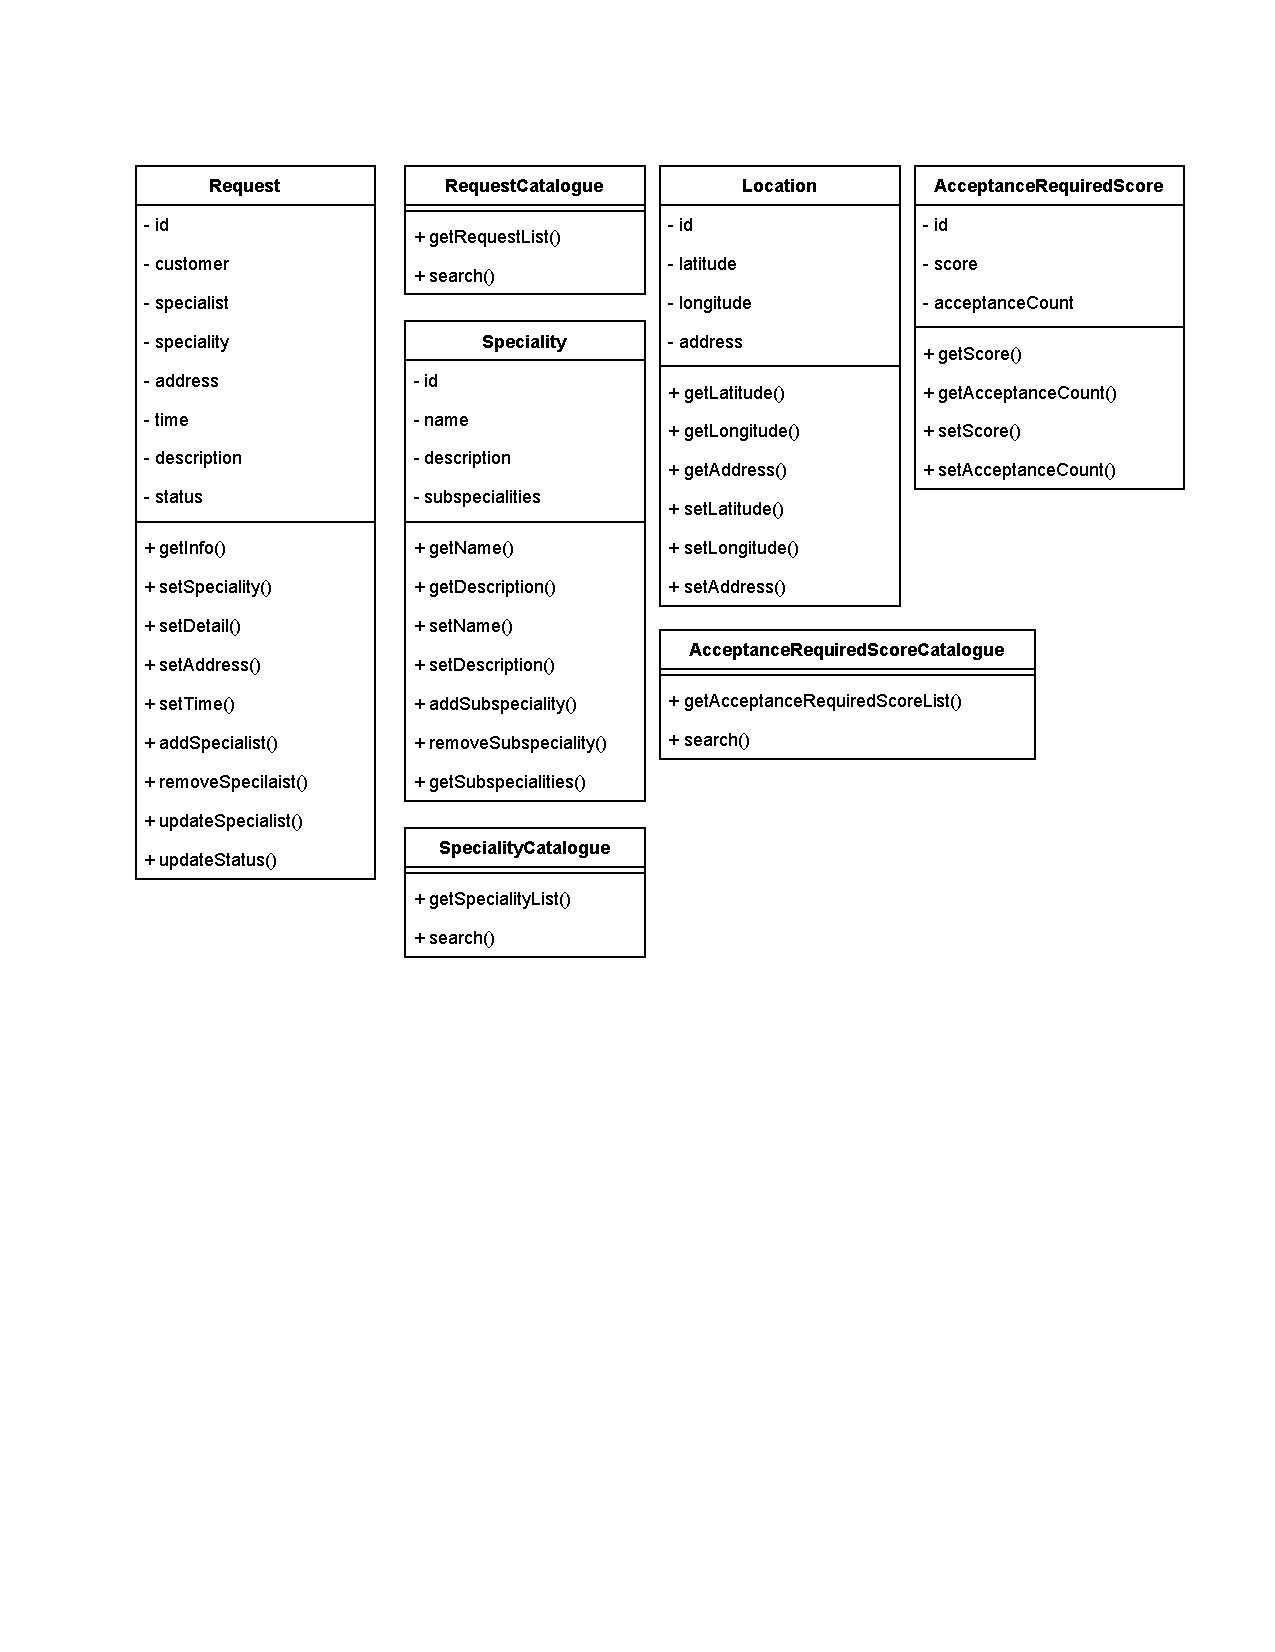
\includegraphics[scale=0.8]{figs/OOD-class-page-1.pdf}
	\caption{نمودار کلاس: کلاس‌های طراحی بخش اول}
\end{figure}
\FloatBarrier
\newpage


\begin{figure}[ht!]
	\centering
	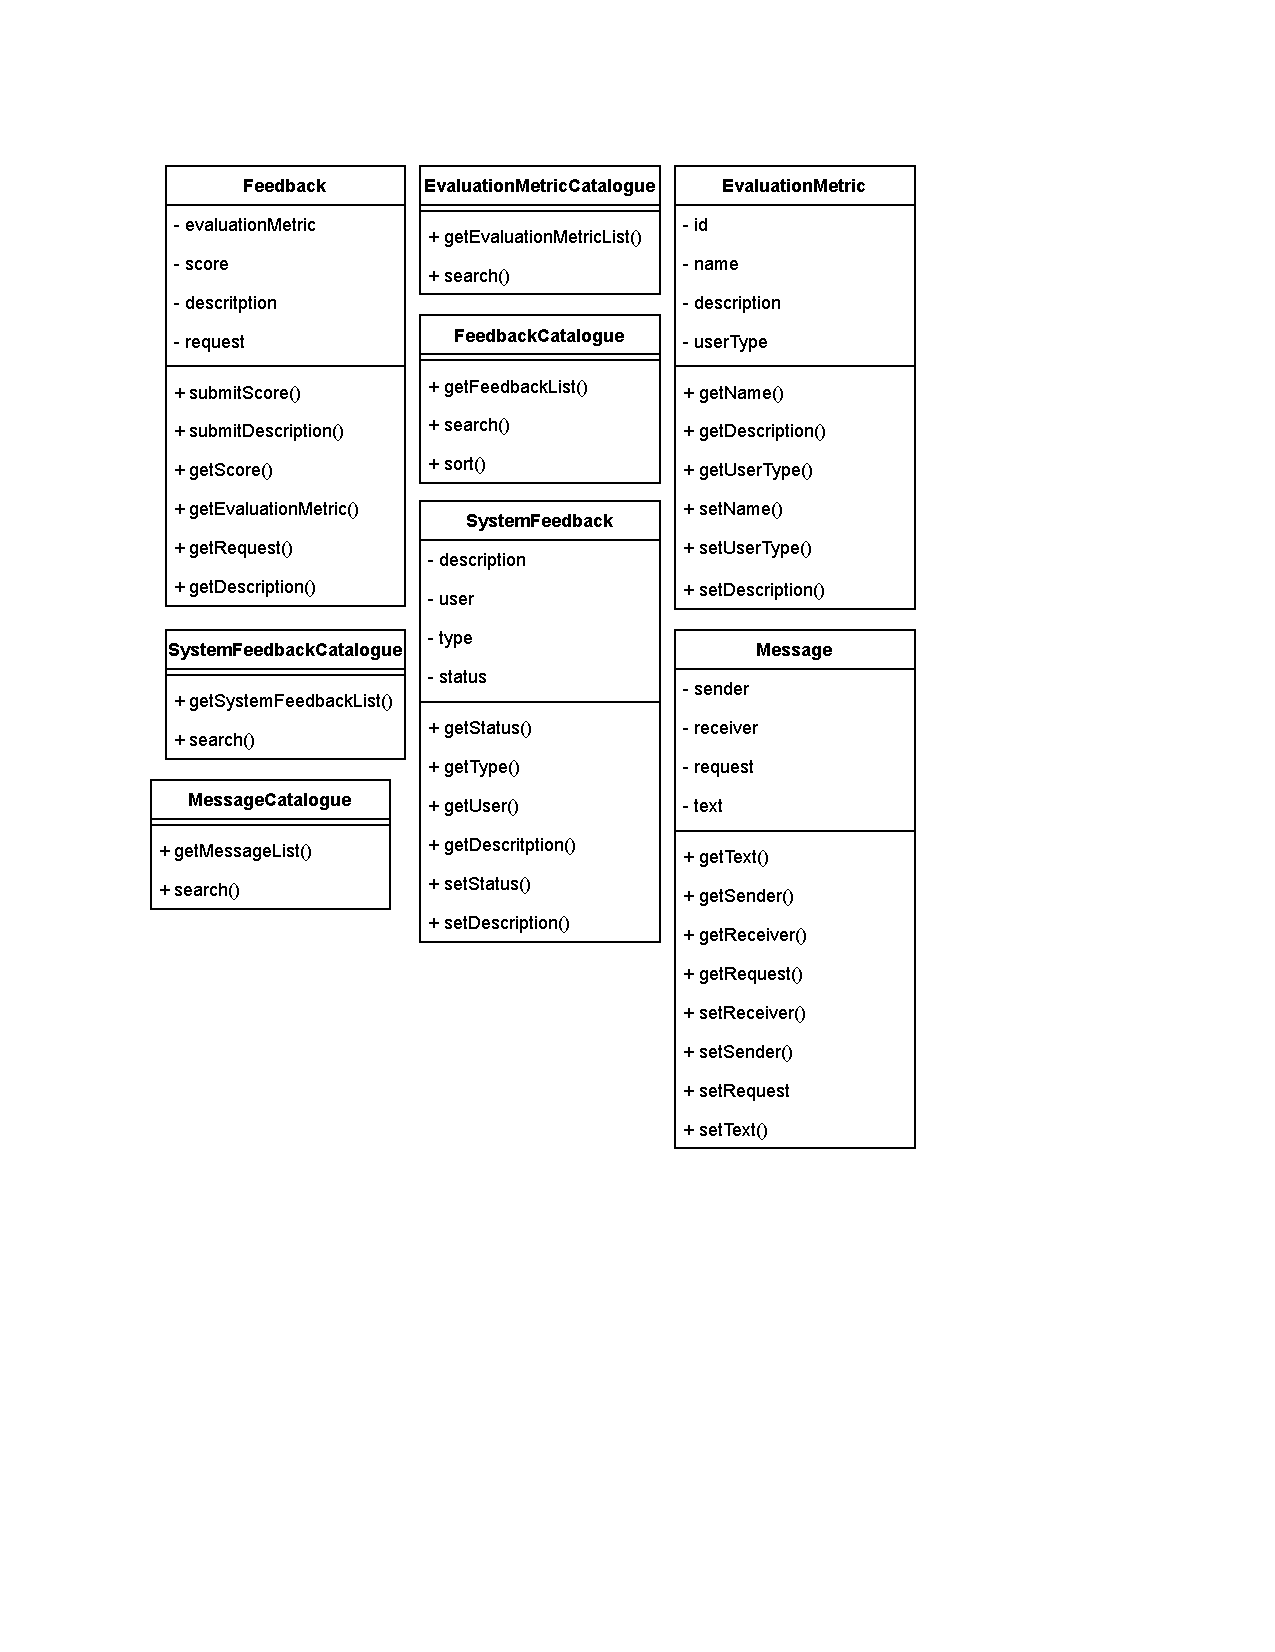
\includegraphics[scale=0.8]{figs/OOD-class-page-2.pdf}
	\caption{نمودار کلاس: کلاس‌های طراحی بخش دوم}
\end{figure}
\FloatBarrier
\newpage

\begin{figure}[ht!]
	\centering
	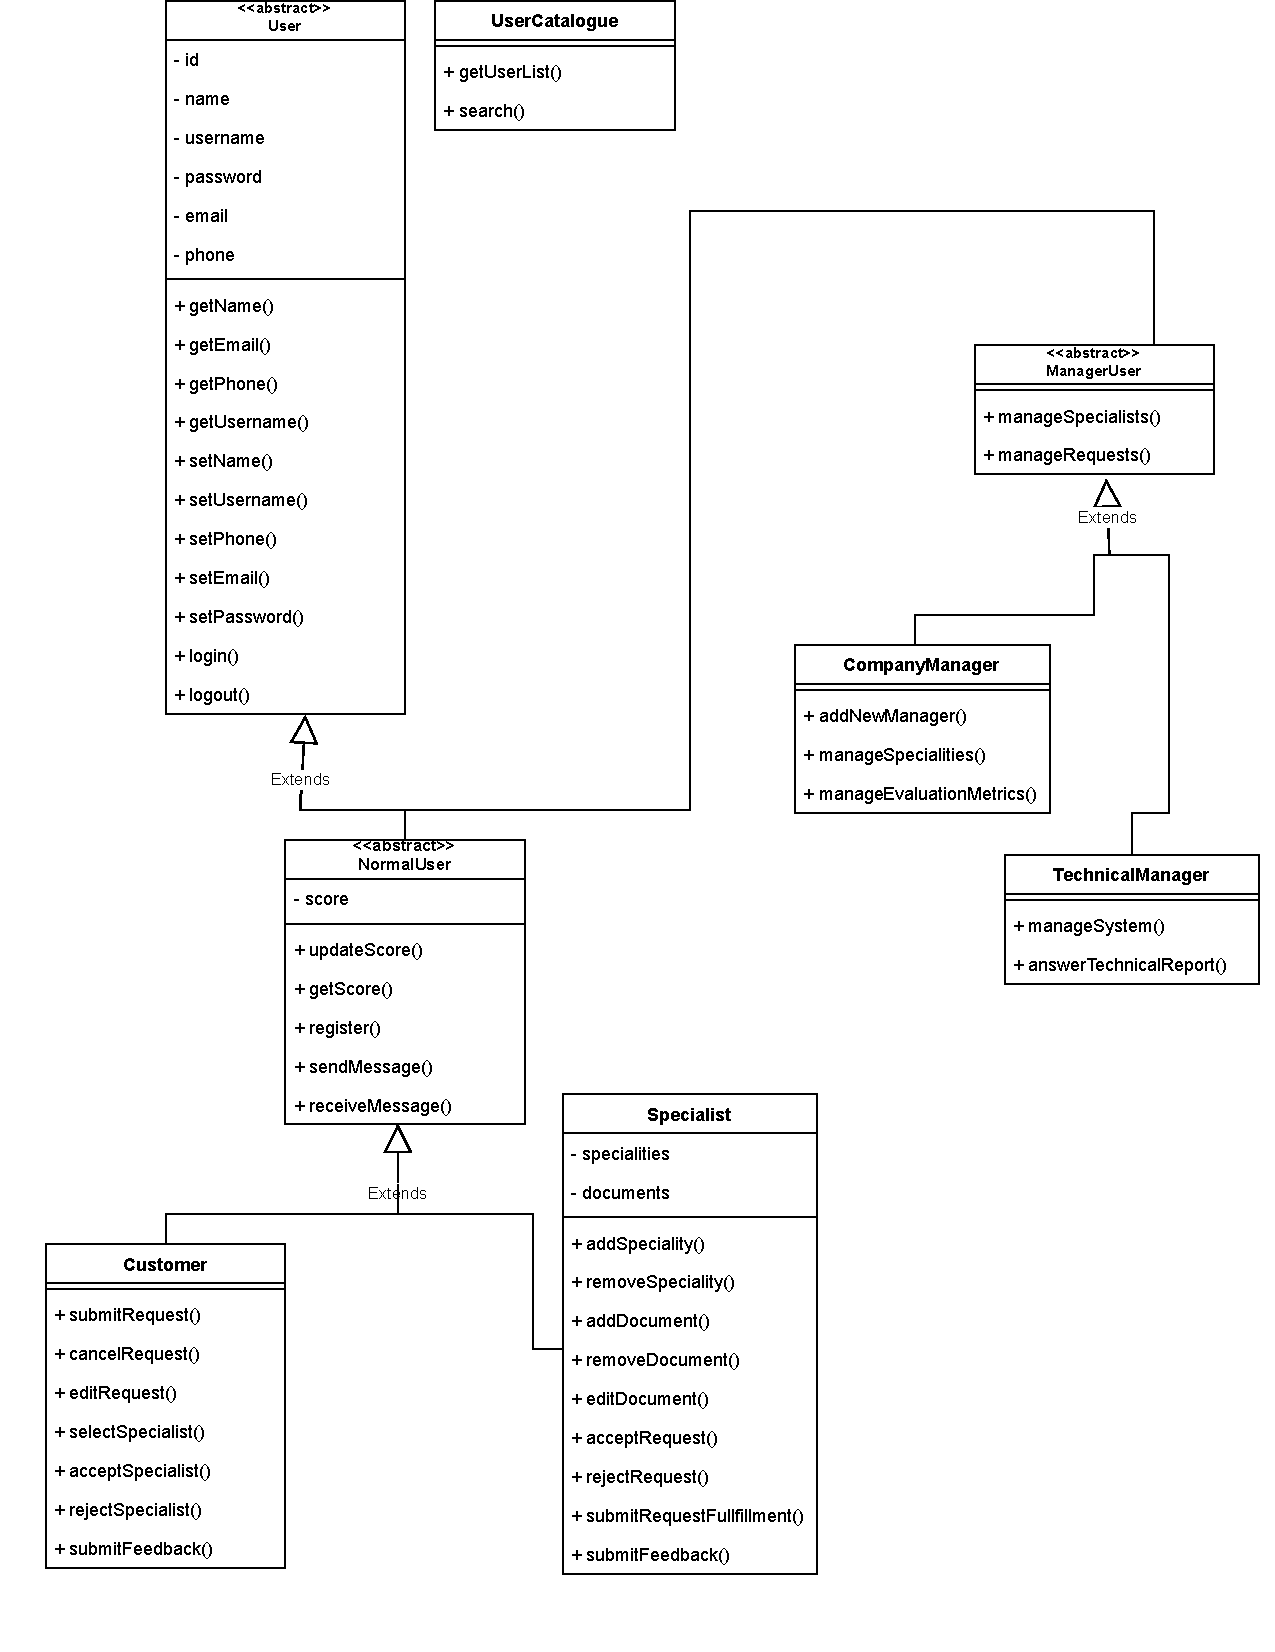
\includegraphics[scale=0.8]{figs/OOD-class-page-3.pdf}
	\caption{نمودار کلاس: کلاس‌های طراحی بخش سوم}
\end{figure}
\FloatBarrier
\newpage

\begin{figure}[ht!]
	\centering
	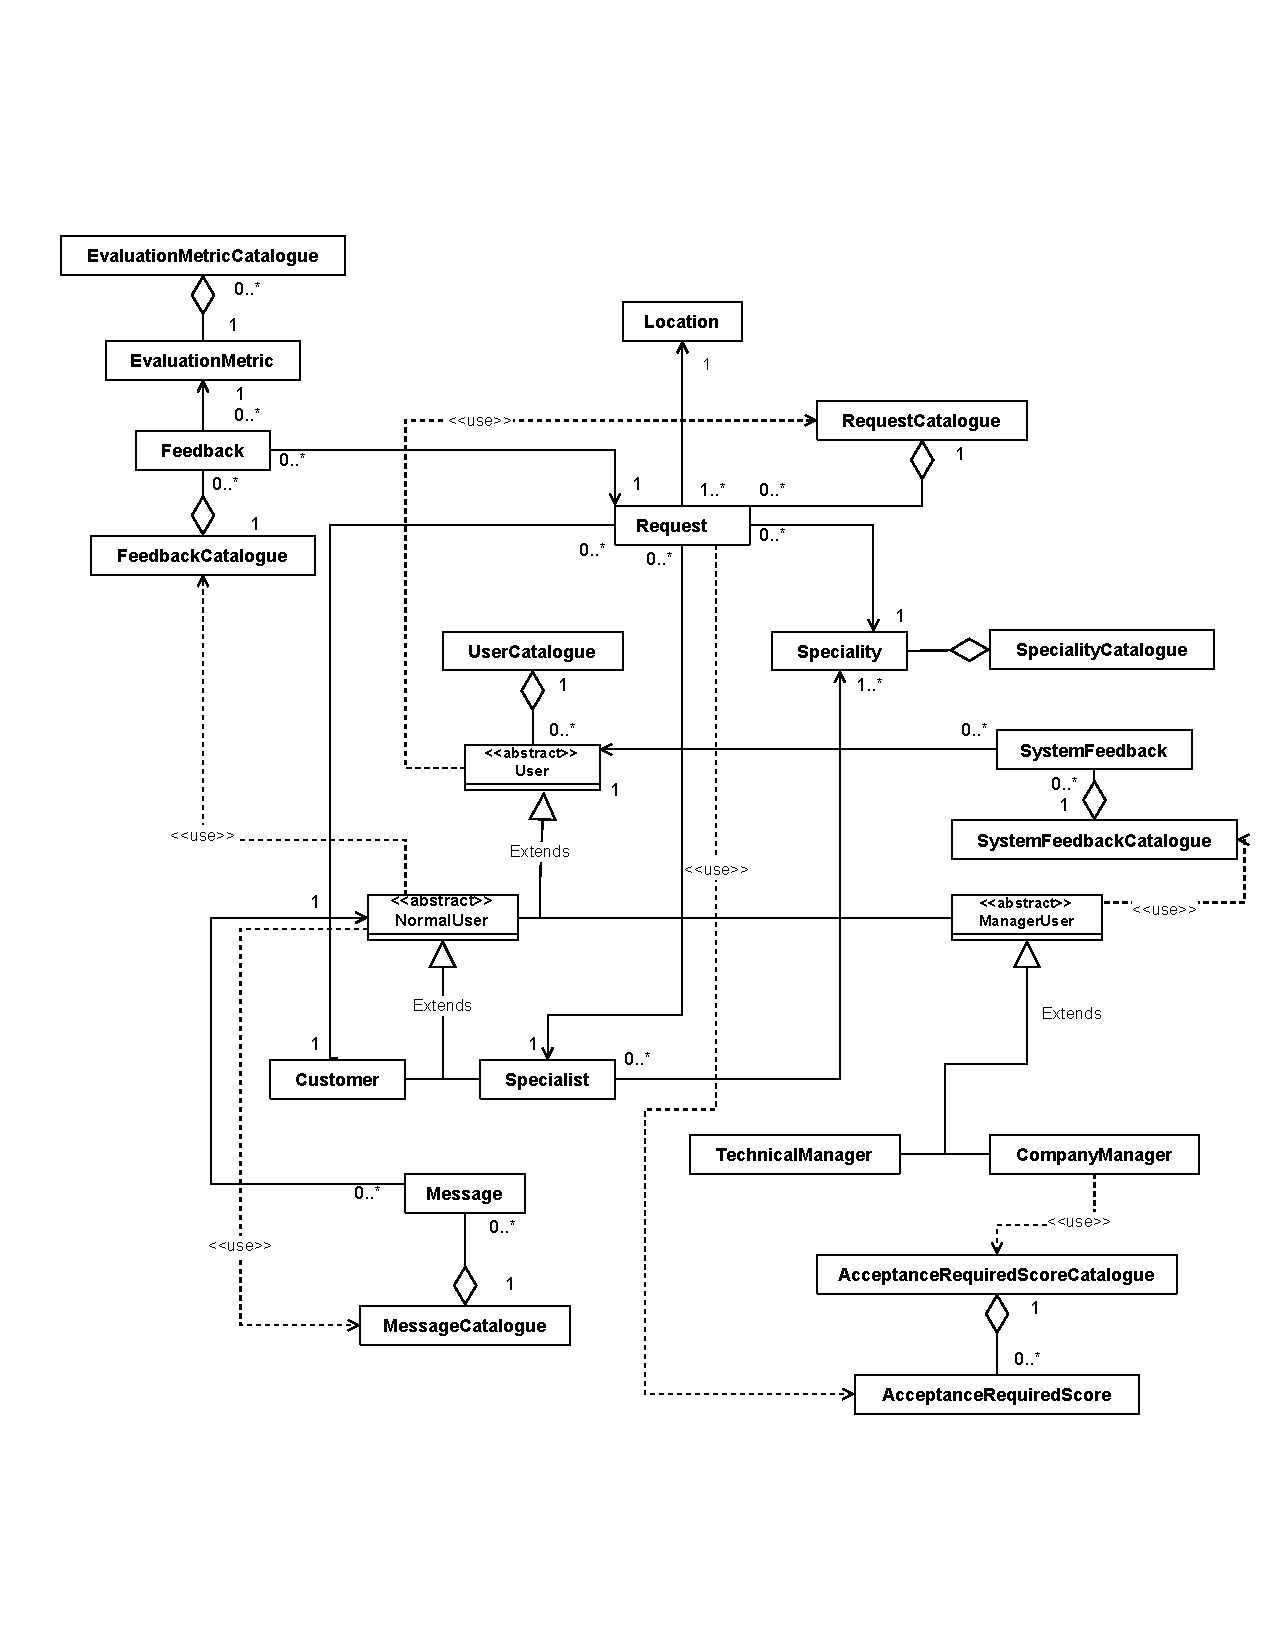
\includegraphics[scale=0.8]{figs/OOD-class-page-4.pdf}
	\caption{نمودار کلاس: ارتباط بین همه کلاس‌ها}
\end{figure}
\FloatBarrier
\newpage
	\chapter{نمودار بسته تحلیل}

در ادامه نمودار بسته‌های تحلیل برای کلاس‌های گفته شده در فصل
\ref{chapter:classAnalysis}
آورده شده است.


\begin{figure}[ht!]
	\centering
	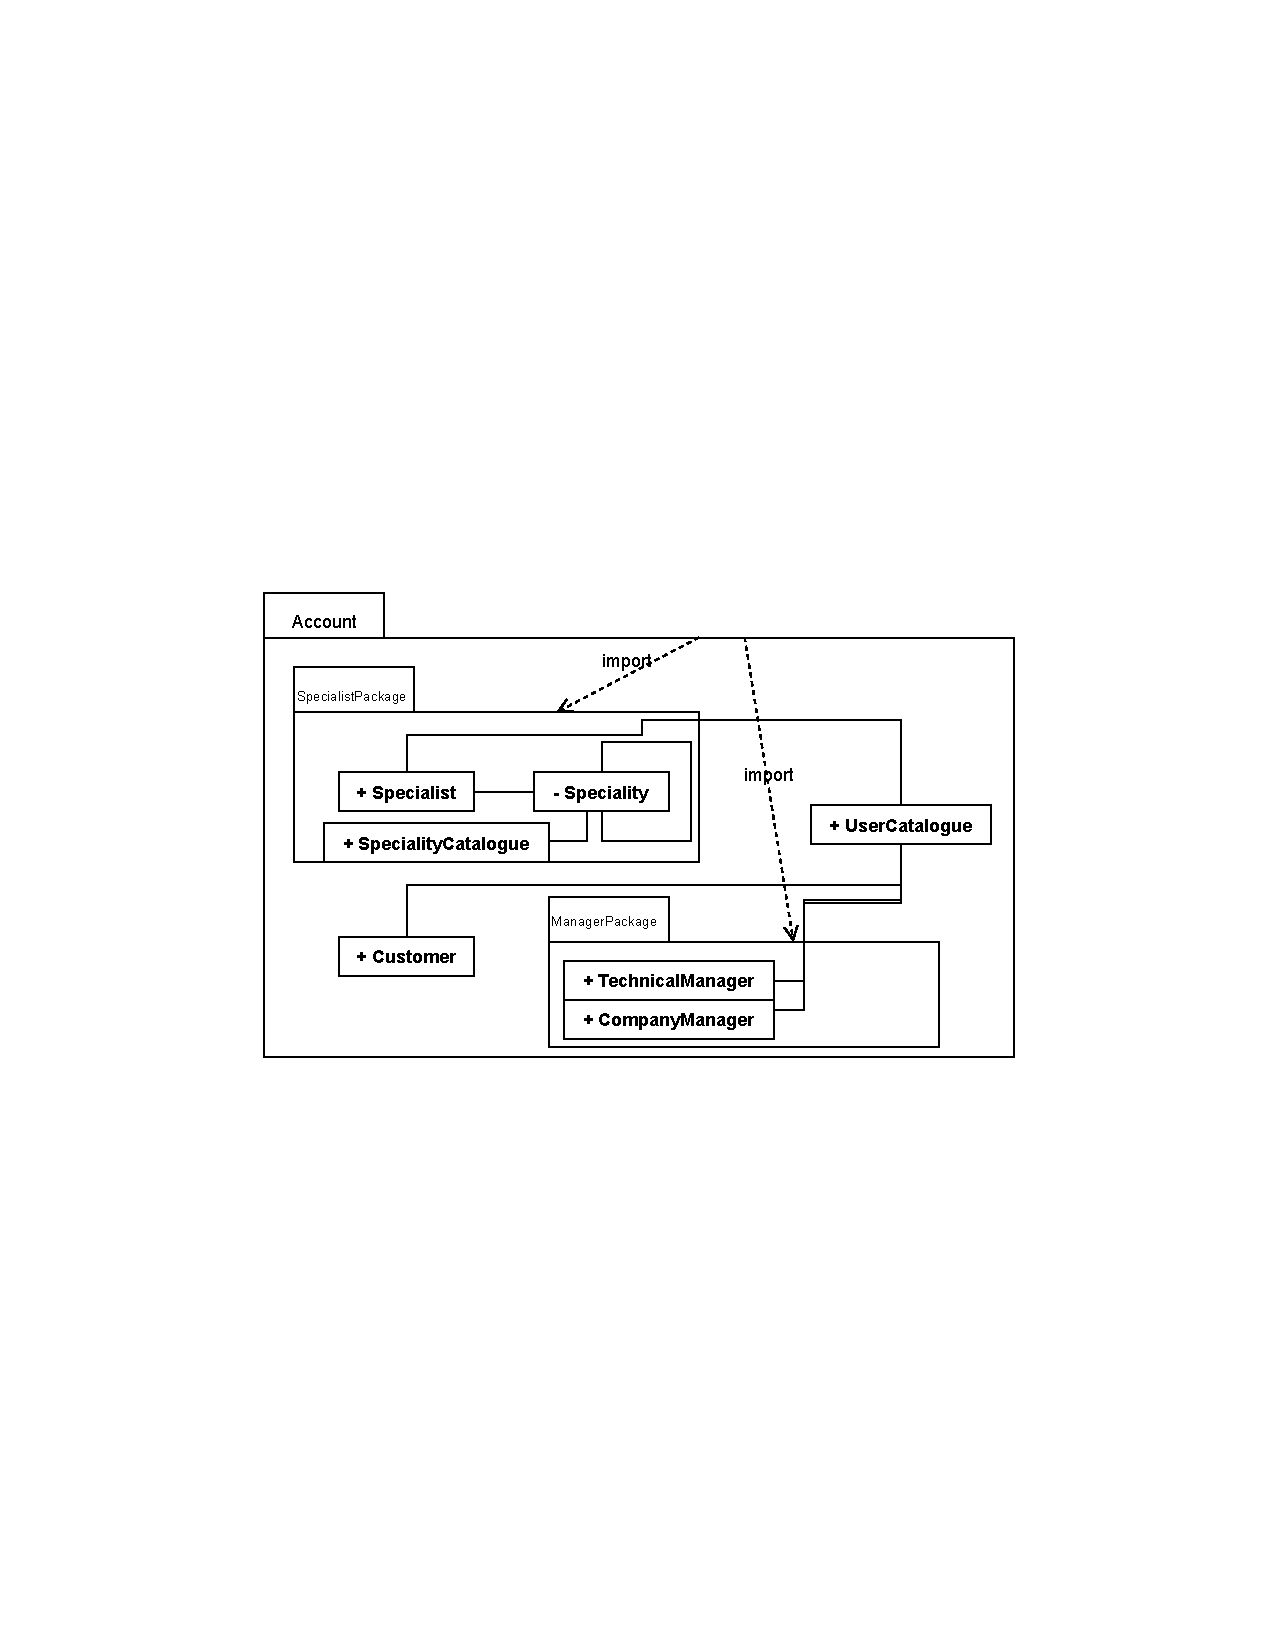
\includegraphics[scale=0.8]{figs/OOD-package-1.pdf}
	\caption{نمودار بسته: بسته \lr{Account}}
\end{figure}
\FloatBarrier
\newpage

\begin{figure}[ht!]
	\centering
	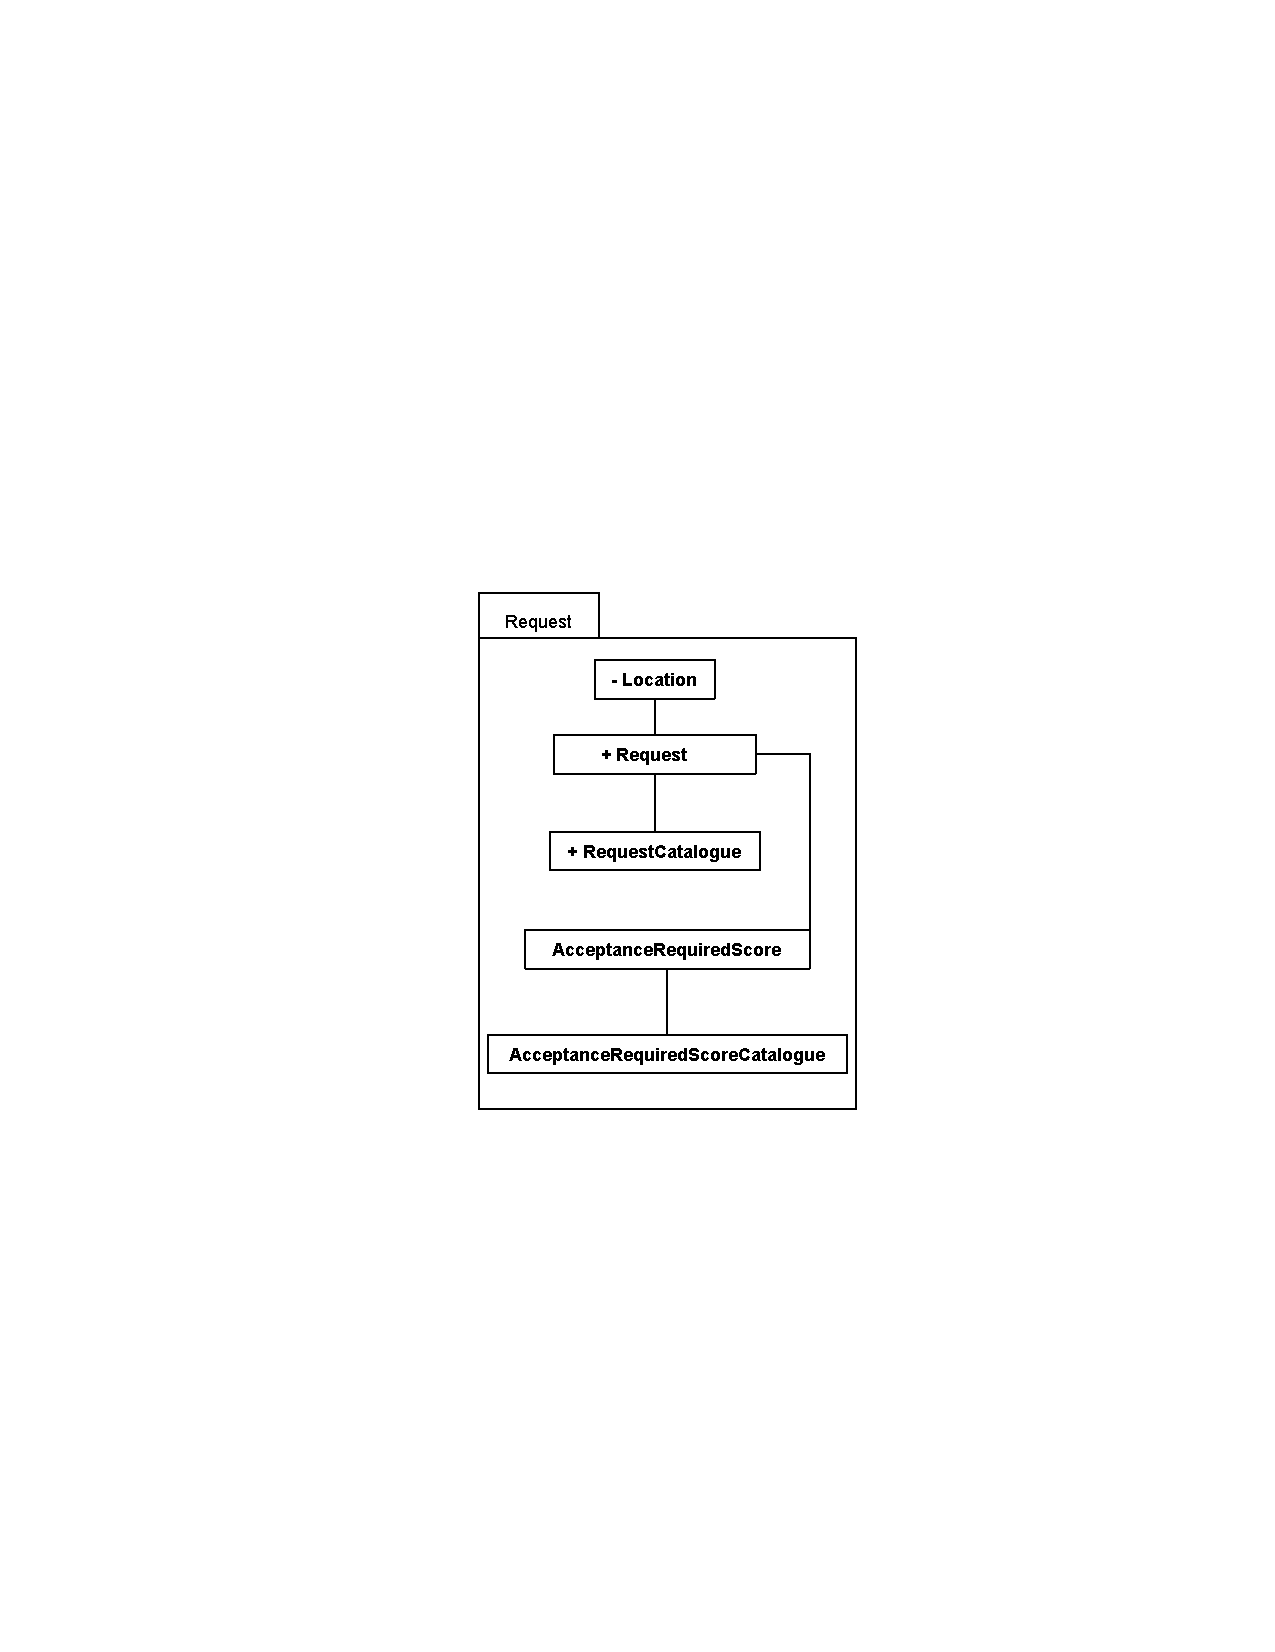
\includegraphics[scale=0.8]{figs/OOD-package-2.pdf}
	\caption{نمودار بسته: بسته \lr{Request}}
\end{figure}
\FloatBarrier
\newpage


\begin{figure}[ht!]
	\centering
	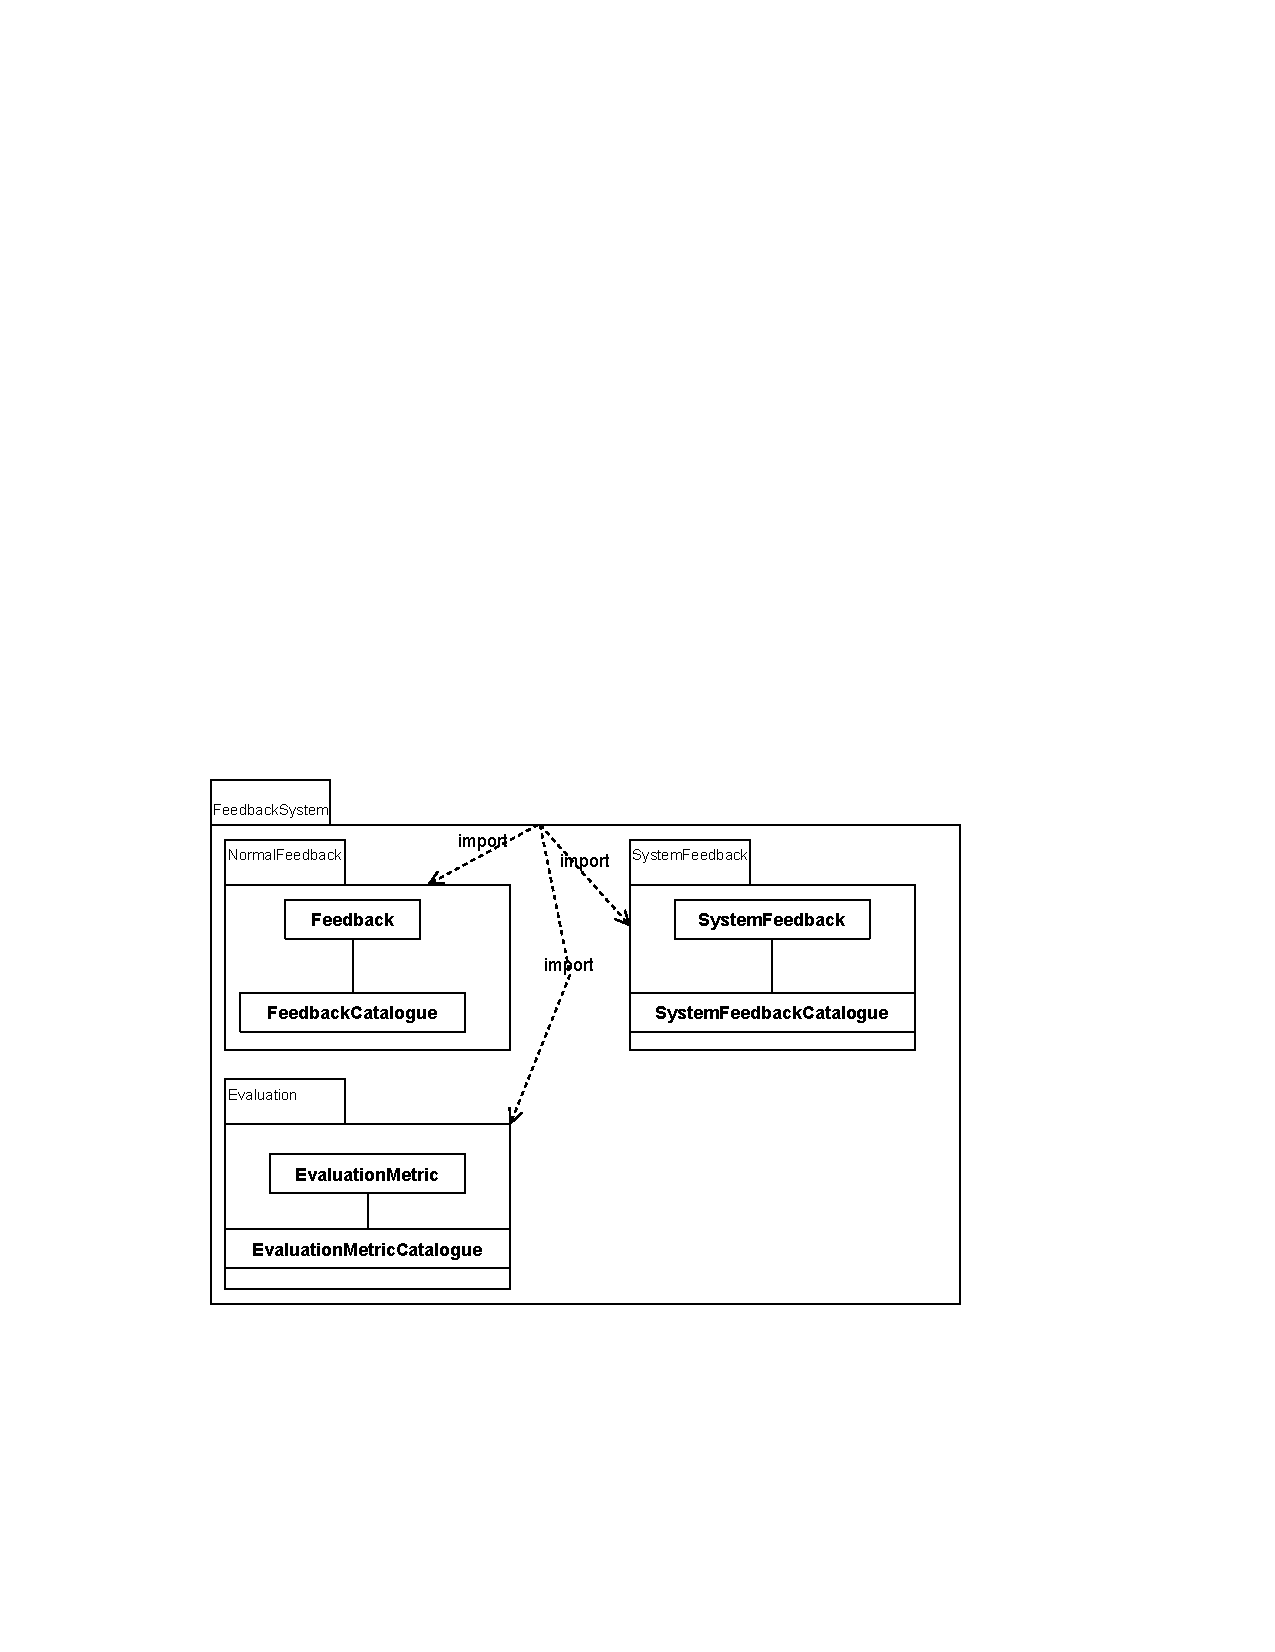
\includegraphics[scale=0.8]{figs/OOD-package-3.pdf}
	\caption{نمودار بسته: بسته \lr{FeedbackSystem}}
\end{figure}
\FloatBarrier
\newpage

\begin{figure}[ht!]
	\centering
	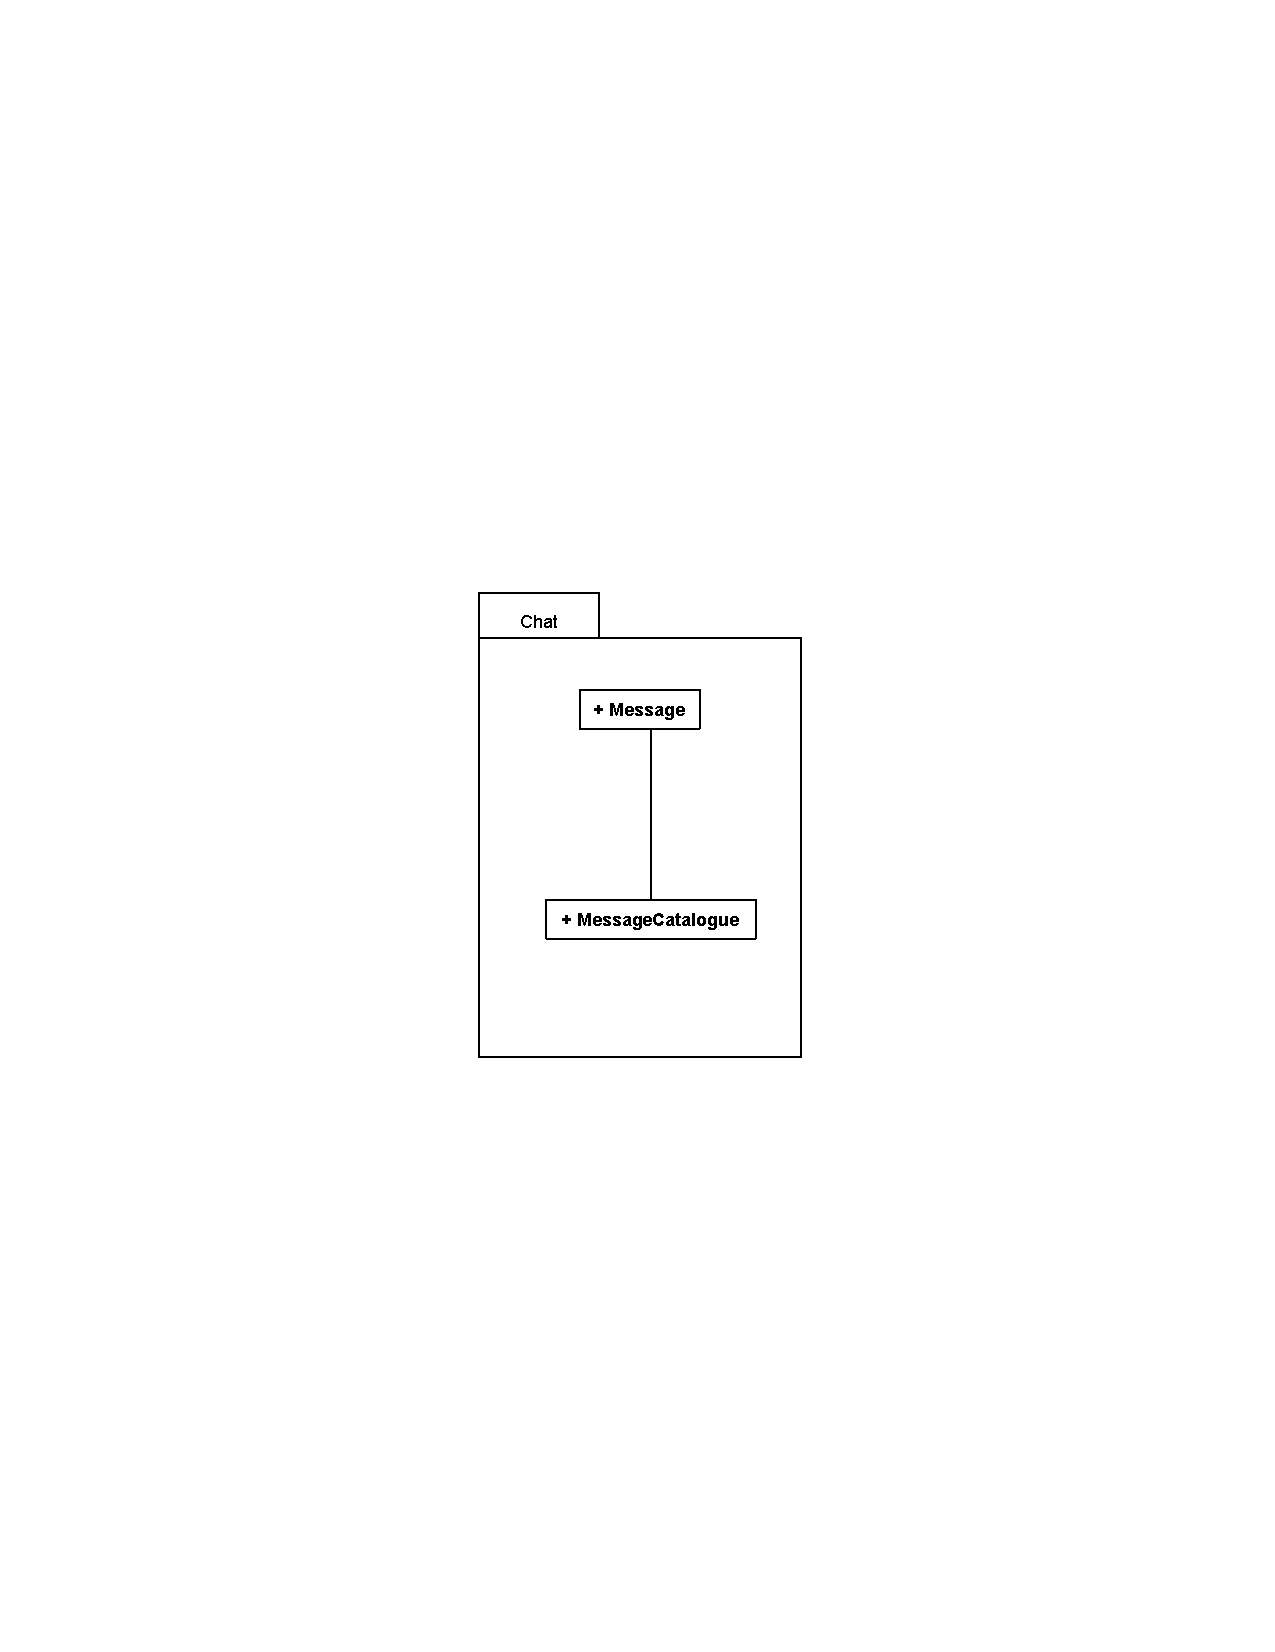
\includegraphics[scale=0.8]{figs/OOD-package-4.pdf}
	\caption{نمودار بسته: بسته \lr{Chat}}
\end{figure}
\FloatBarrier
\newpage

\begin{figure}[ht!]
	\centering
	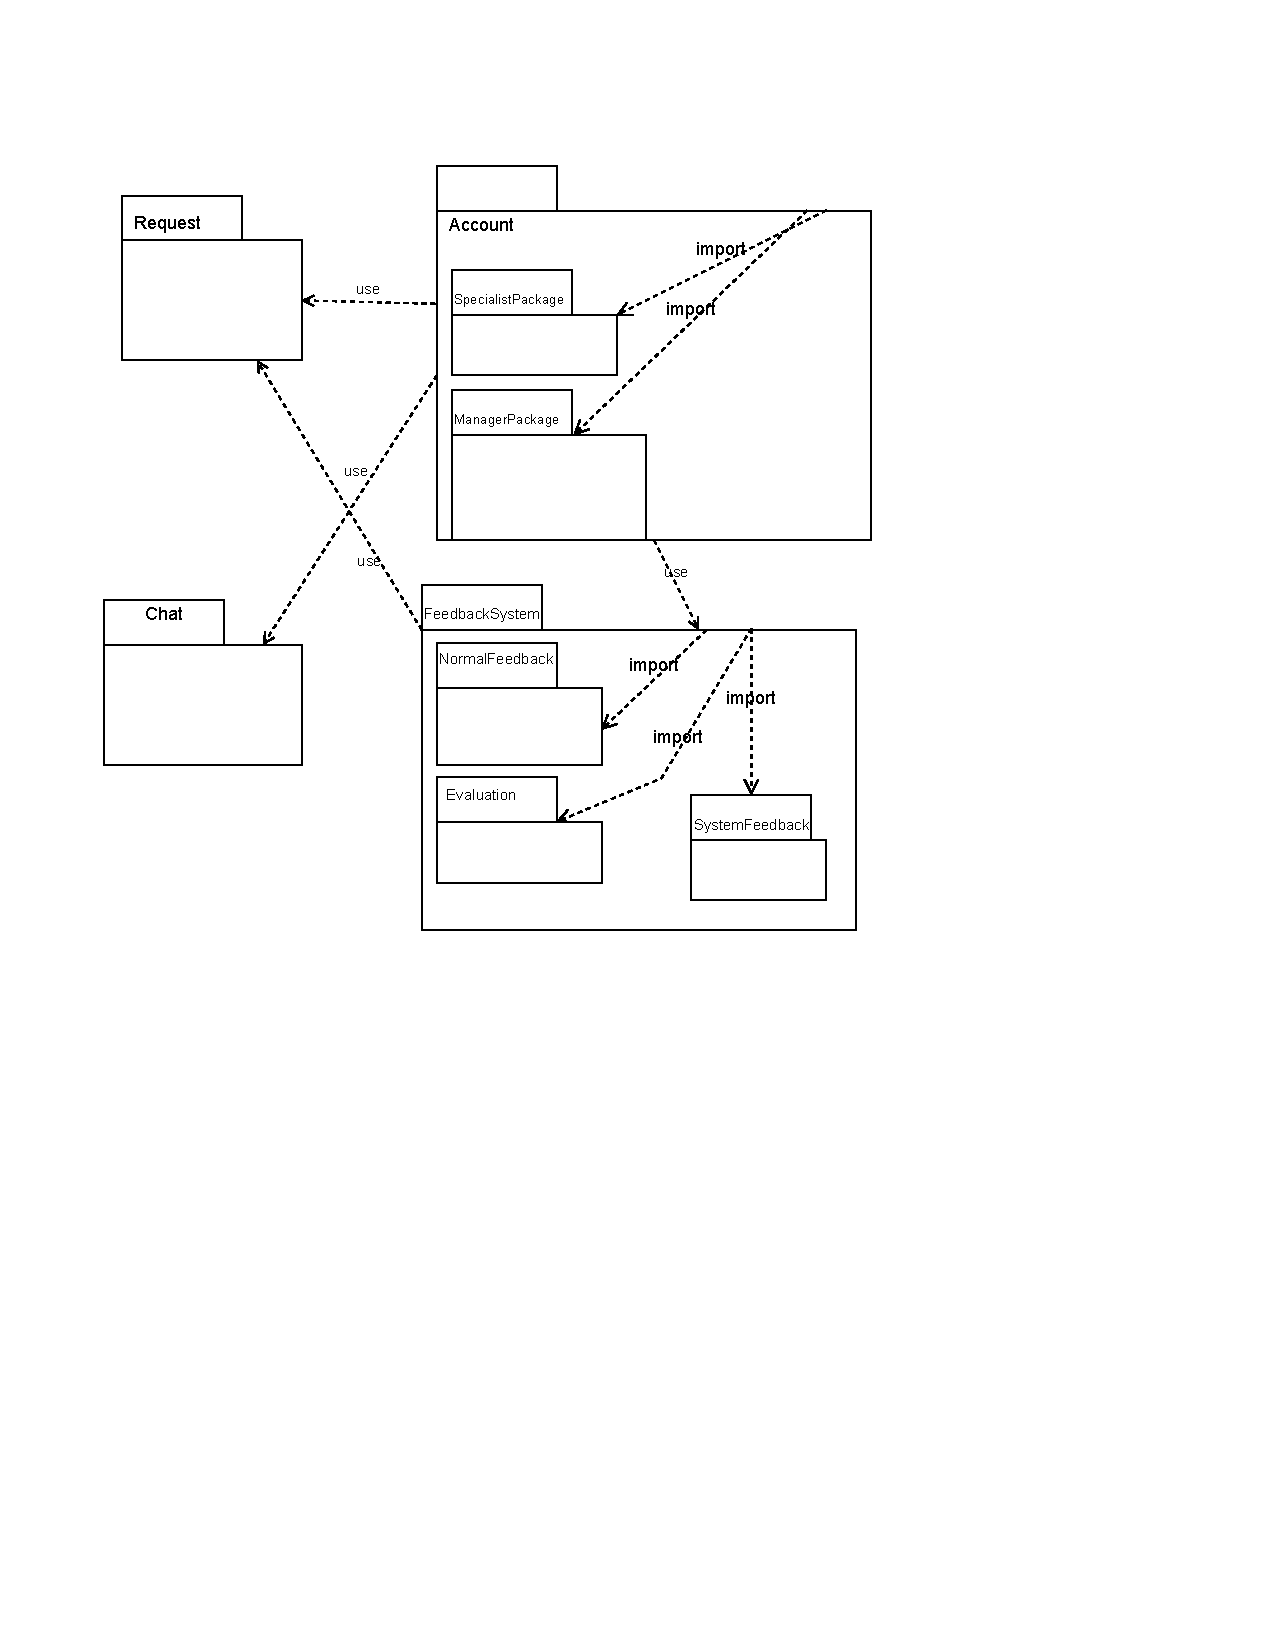
\includegraphics[scale=0.8]{figs/OOD-package-5.pdf}
	\caption{نمودار بسته:  ارتباط بسته‌ها با یکدیگر}
\end{figure}
\FloatBarrier
\newpage


	\chapter{نمودارهای فعالیت}

نمودارهای فعالیت مربوط به هریک از موارد کاربرد (با نام مشابه) به تفکیک زیرسیستم در این بخش ارائه می‌شود.

همچنین لازم به ذکر است از ذکر پیش‌نیازها و پس‌نیازها در نمودارهای فعالیت به‌دلیل تطابق کامل آن‌ها با پیش‌نیاز‌ها و پس‌نیازهای جداول توصیف موارد کاربرد صرف‌نظر شد.
\newpage
\section{زیرسیستم کاربری}

\begin{figure}[ht!]
	\centering
	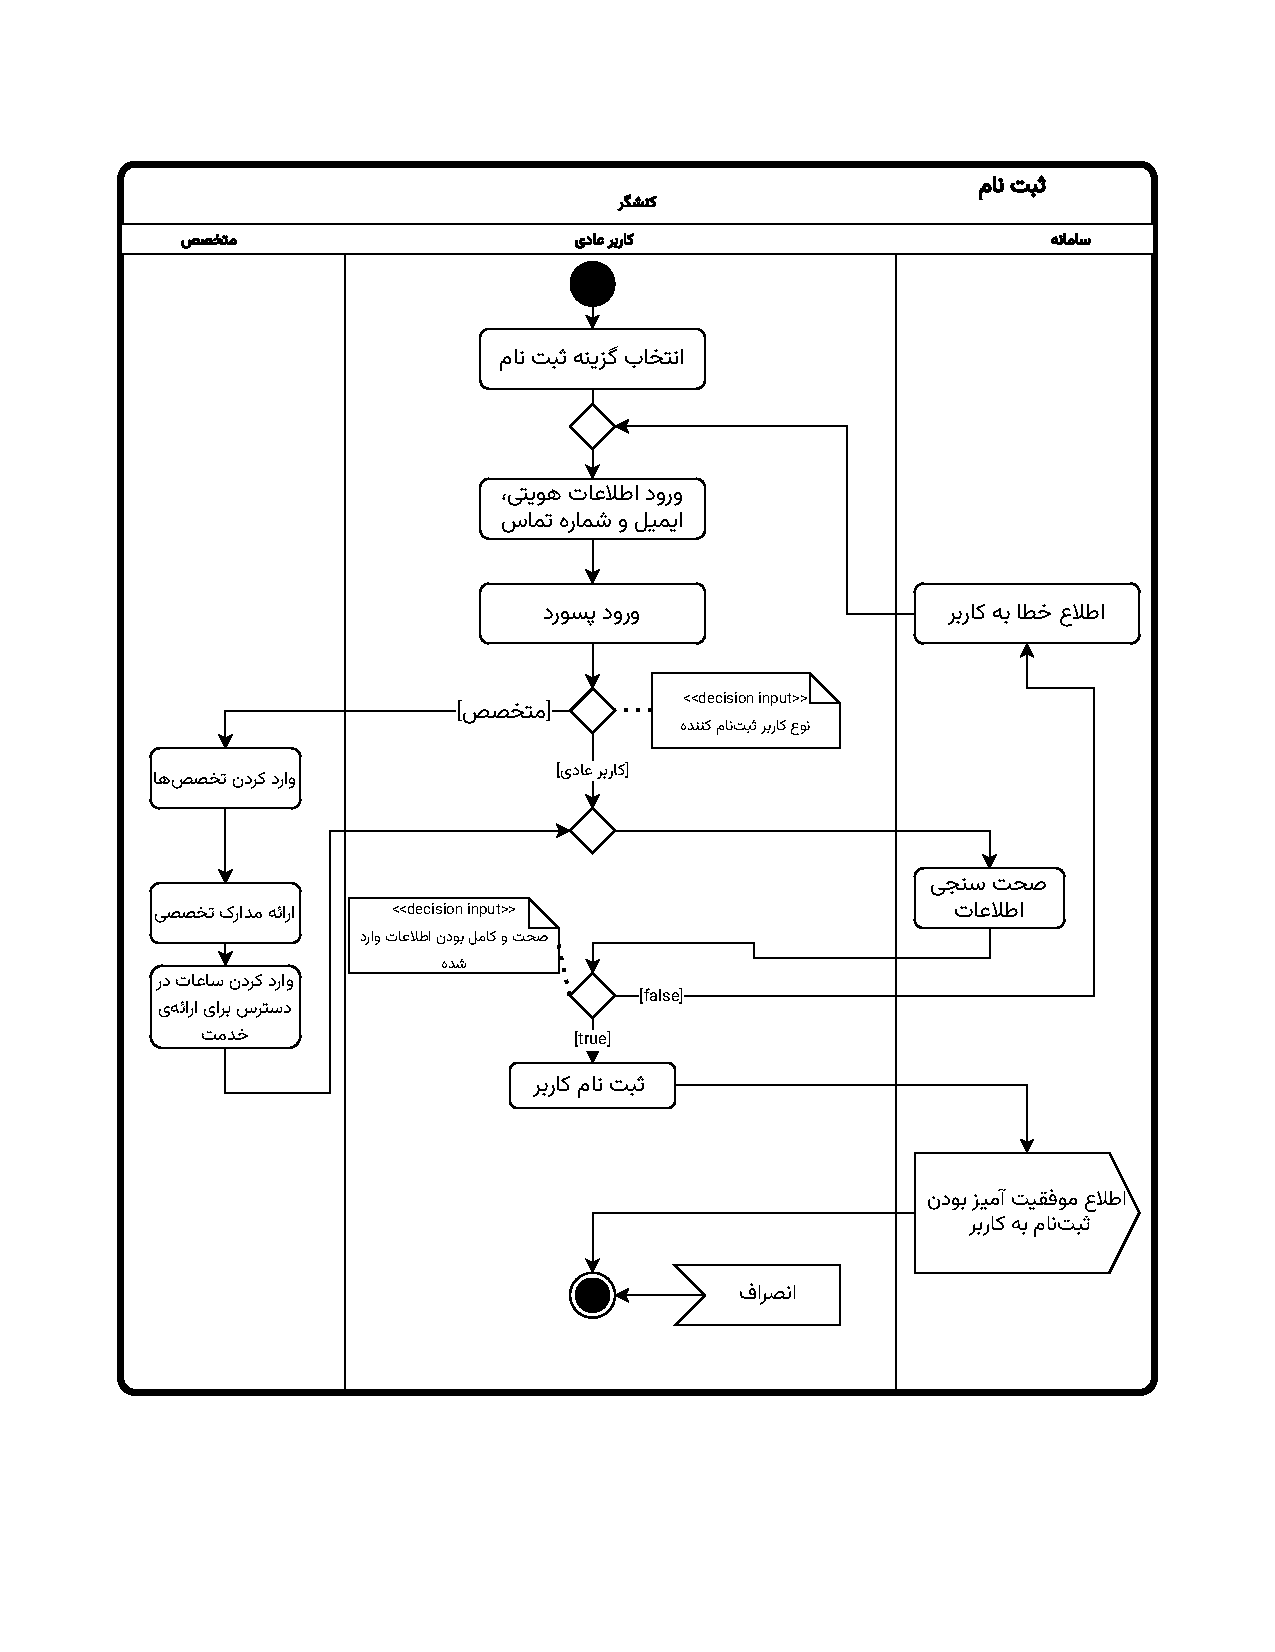
\includegraphics[scale=0.6, page=1]{figs/OOD-activity-signup.pdf}
	\caption{نمودار فعالیت: ثبت نام}
\end{figure}
\FloatBarrier
\newpage

\begin{figure}[ht!]
	\centering
	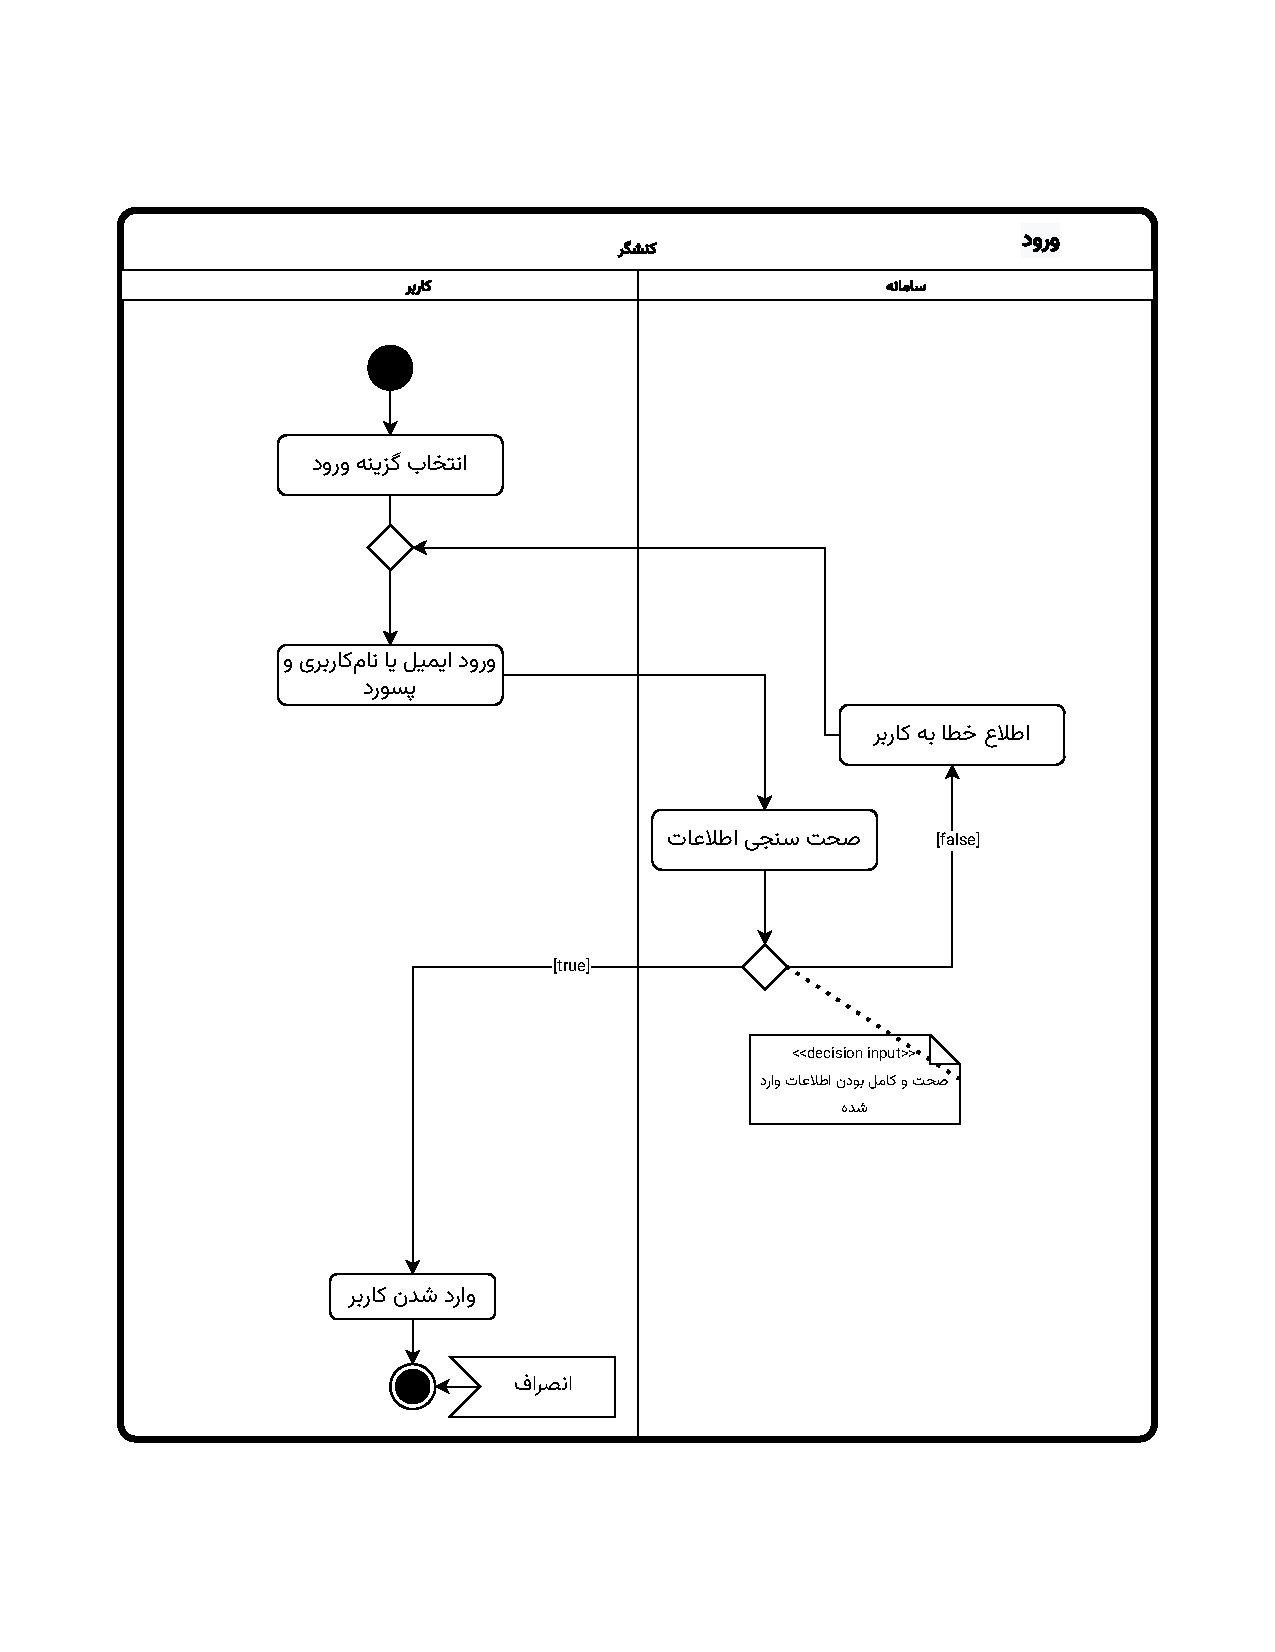
\includegraphics[scale=0.8, page=1]{figs/OOD-activity-login.pdf}
	\caption{نمودار فعالیت: ورود}
\end{figure}
\FloatBarrier
\newpage

\begin{figure}[ht!]
	\centering
	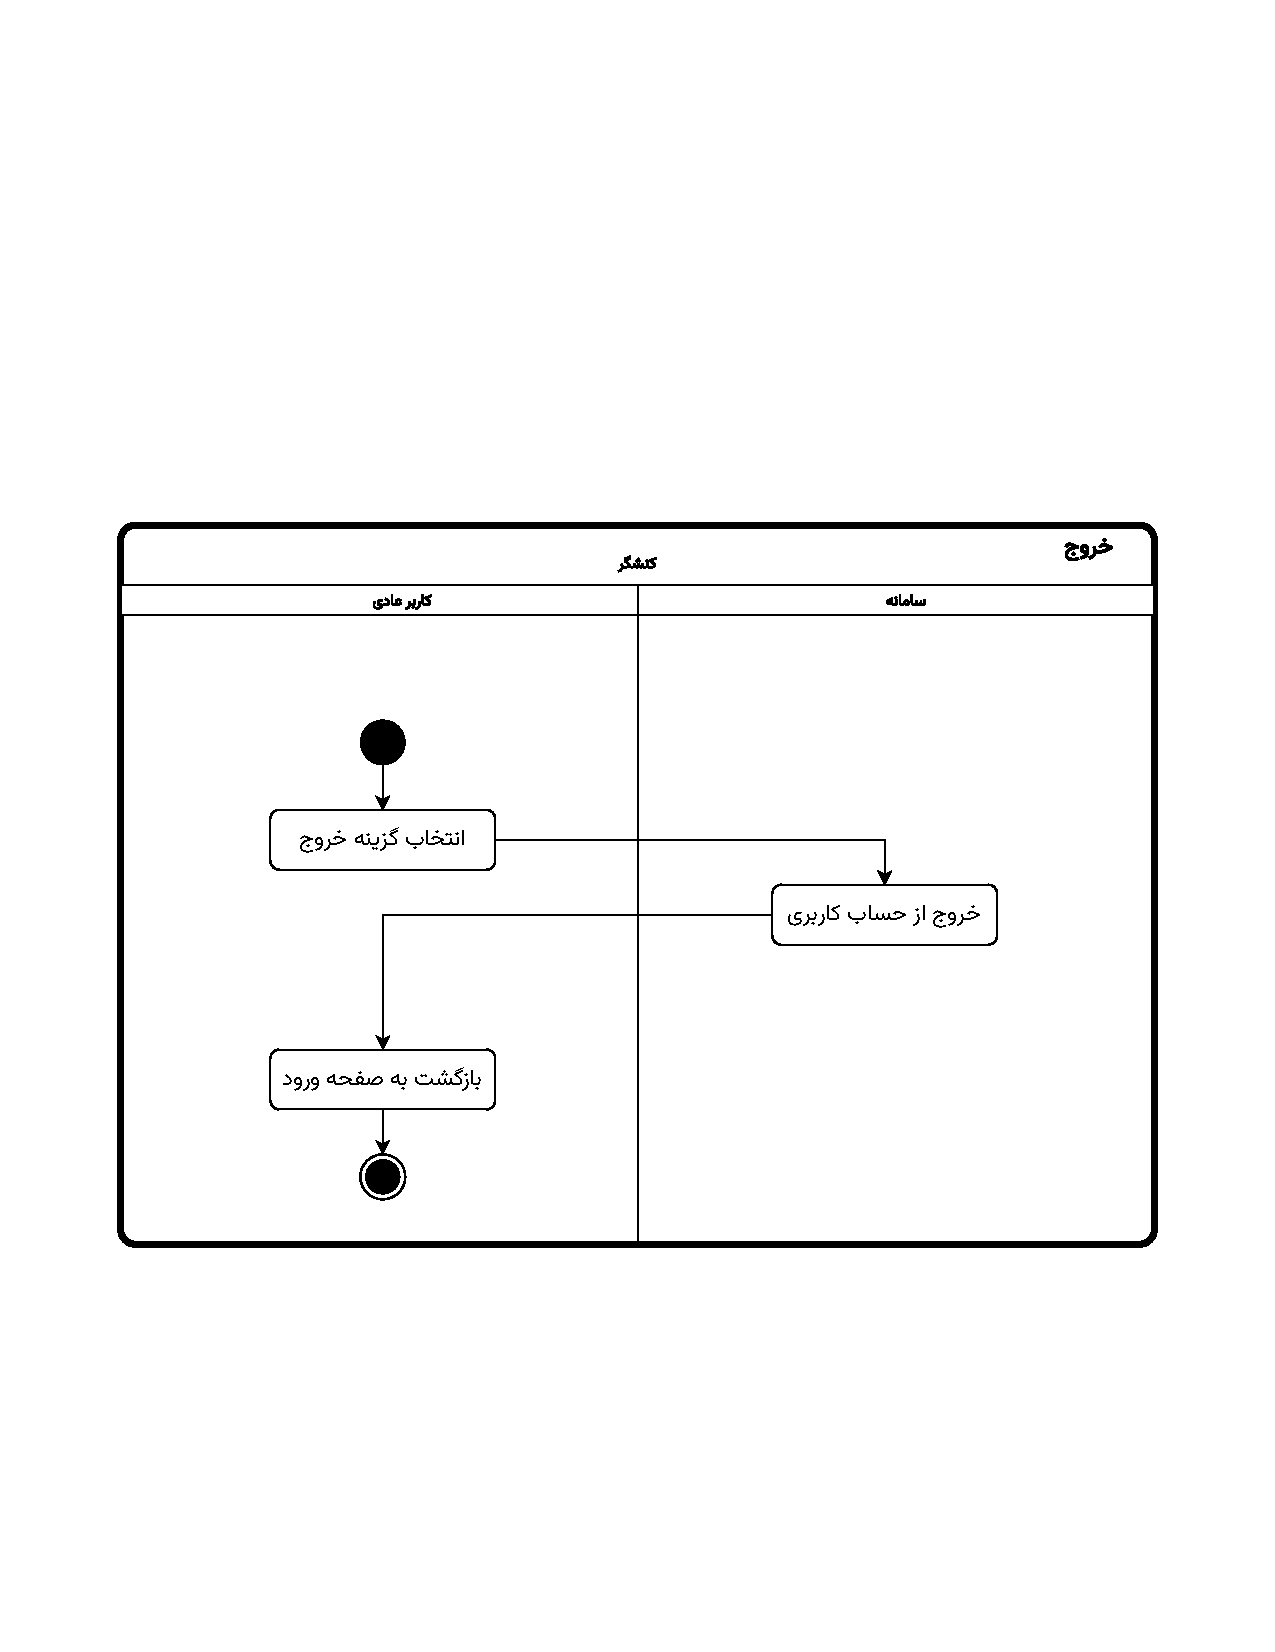
\includegraphics[scale=0.8, page=1]{figs/OOD-activity-logout.pdf}
	\caption{نمودار فعالیت: خروج}
\end{figure}
\FloatBarrier
\newpage

\begin{figure}[ht!]
	\centering
	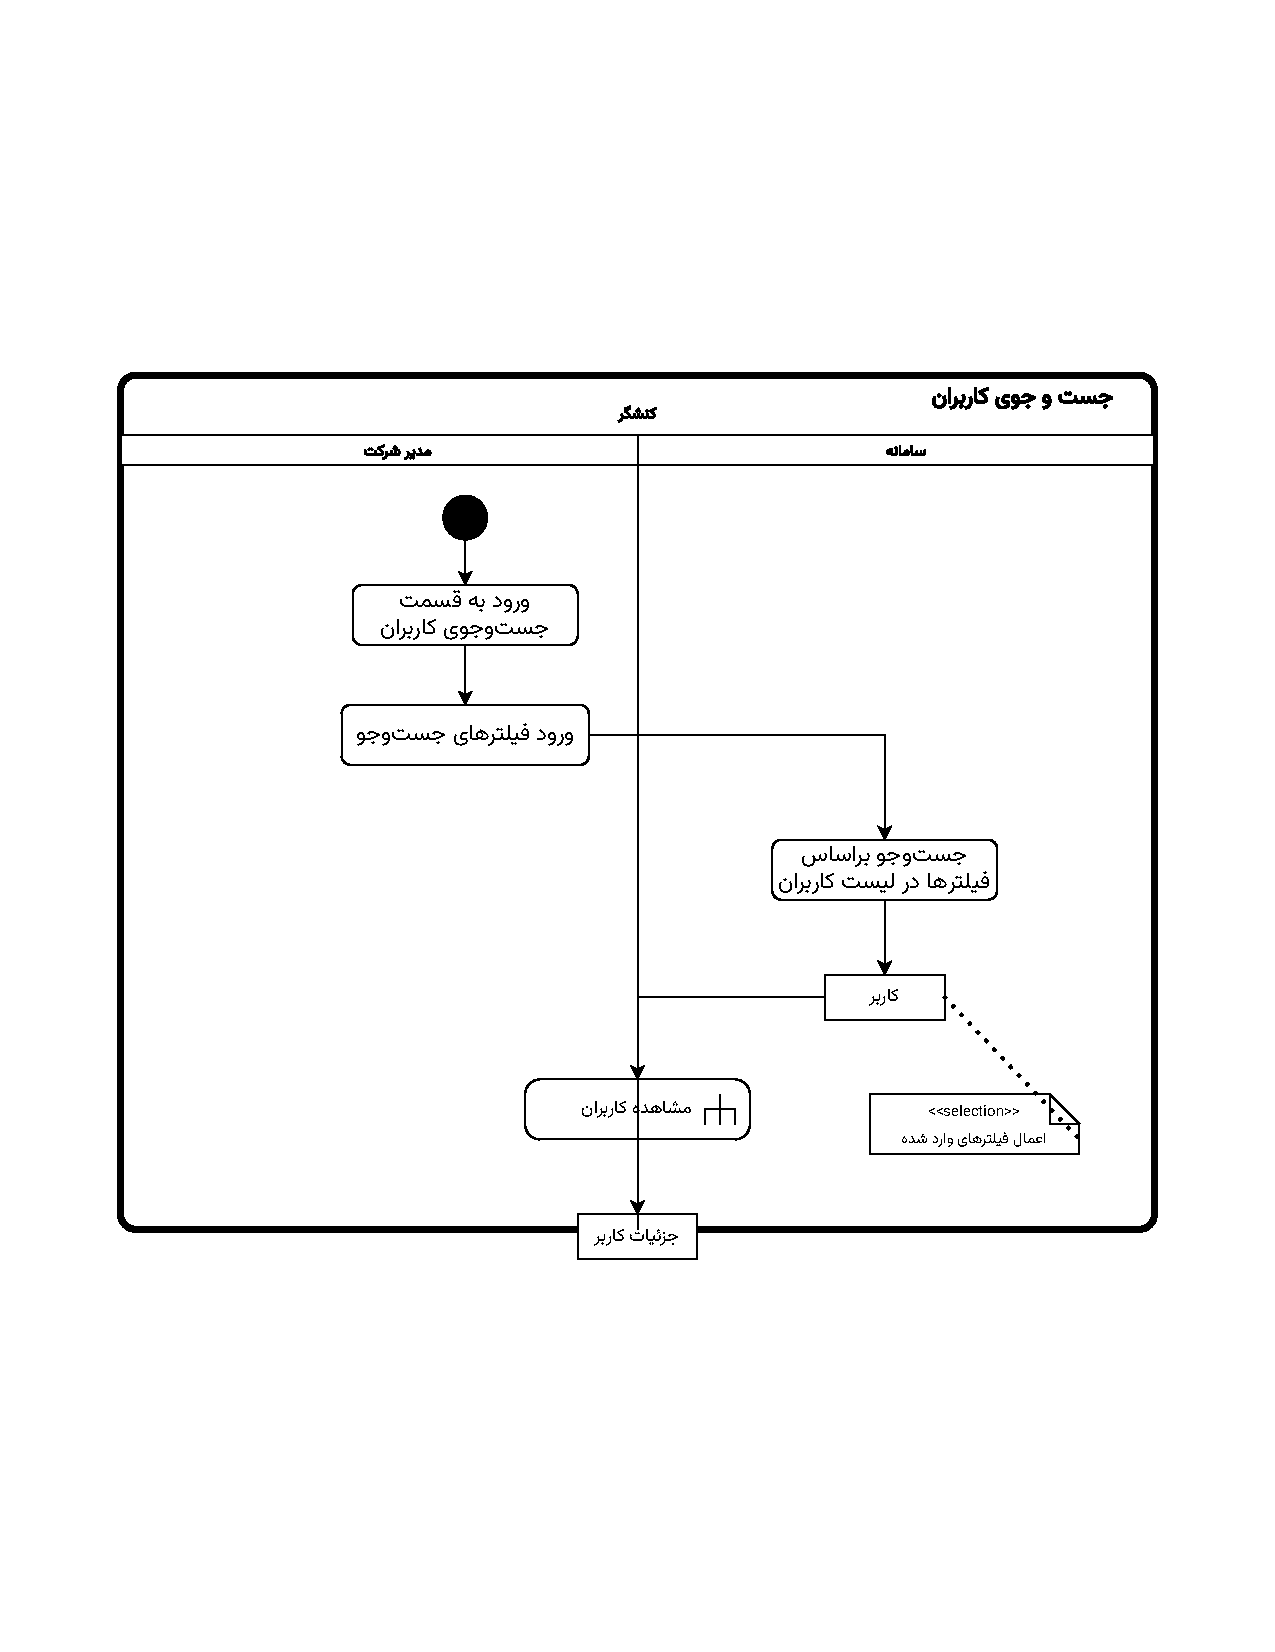
\includegraphics[scale=0.8, page=1]{figs/OOD-activity-searchuser.pdf}
	\caption{نمودار فعالیت: جست‌وجوی کاربران}
\end{figure}
\FloatBarrier
\newpage

\begin{figure}
	\centering
	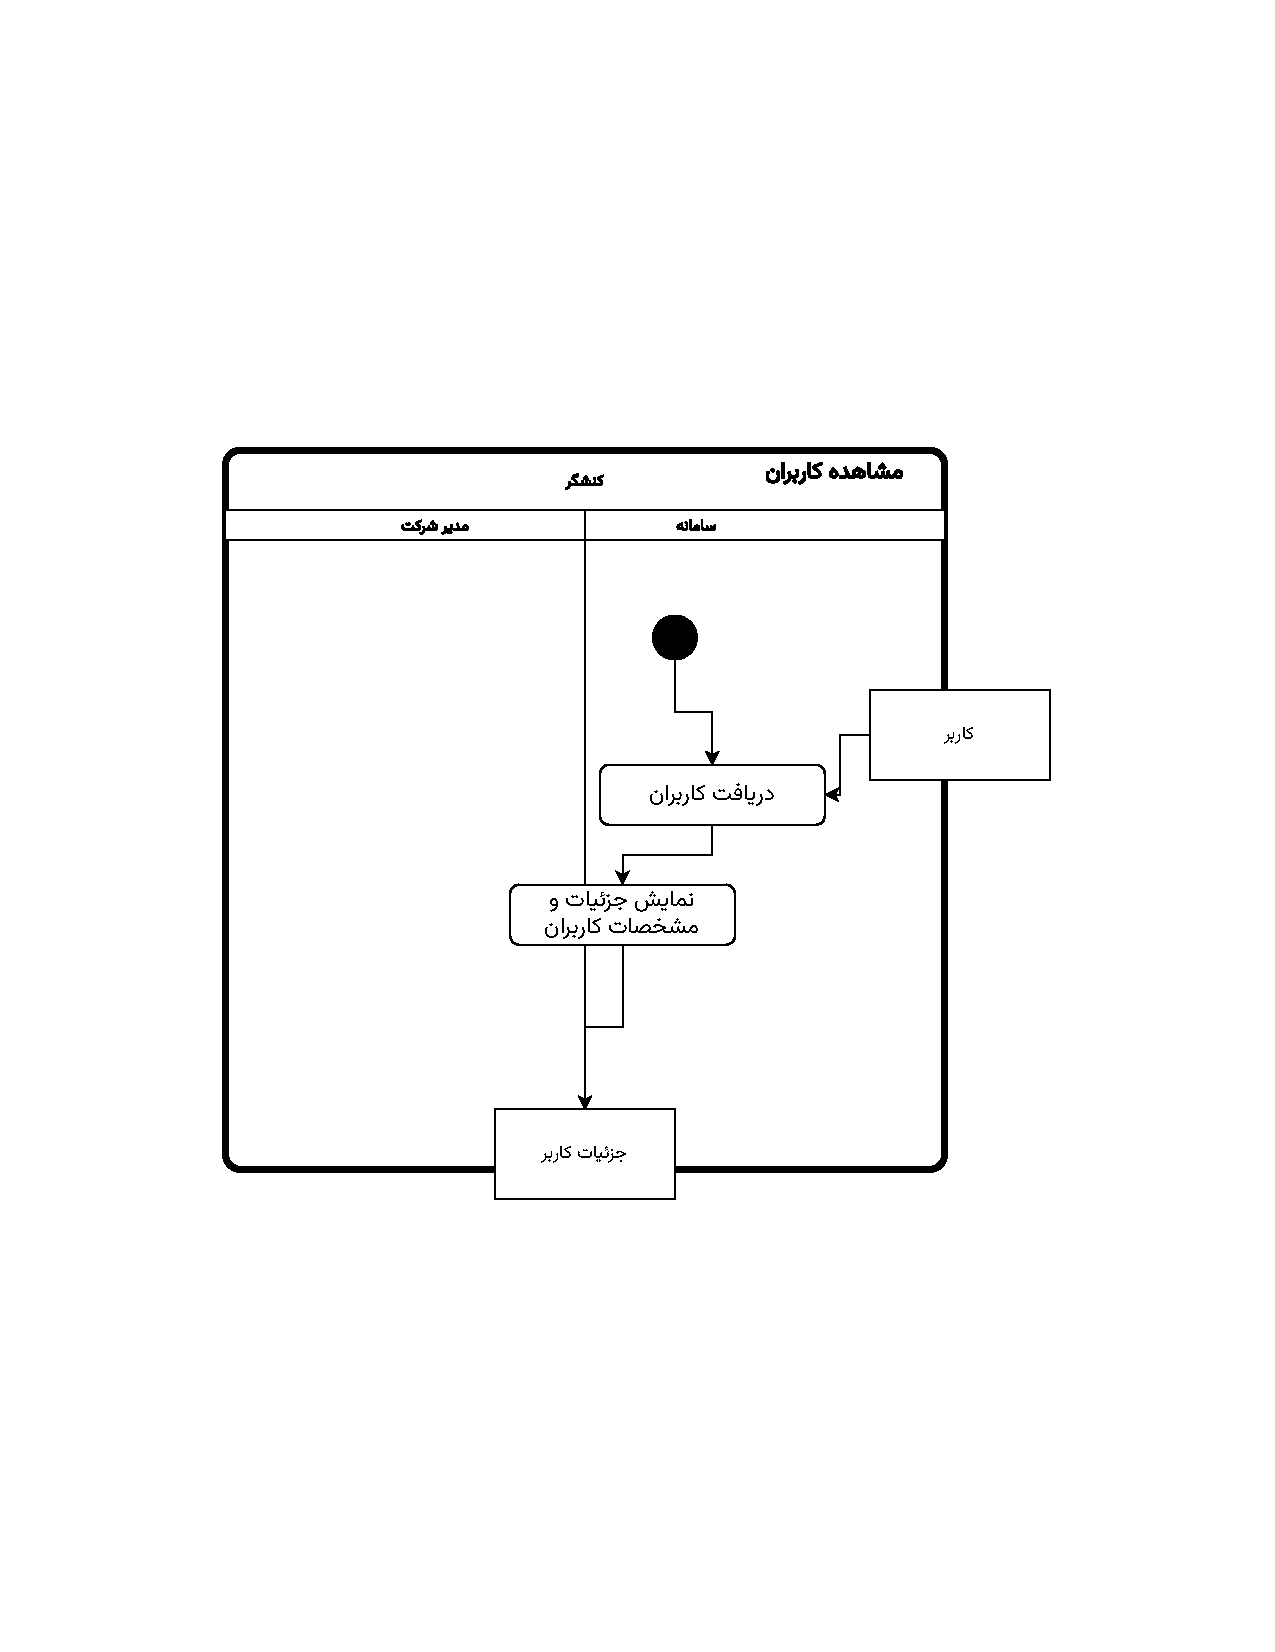
\includegraphics[scale=0.8, page=1]{figs/OOD-activity-viewuser.pdf}
	\caption{نمودار فعالیت: مشاهده کاربران}
\end{figure}
\FloatBarrier
\newpage

\begin{figure}[ht!]
	\centering
	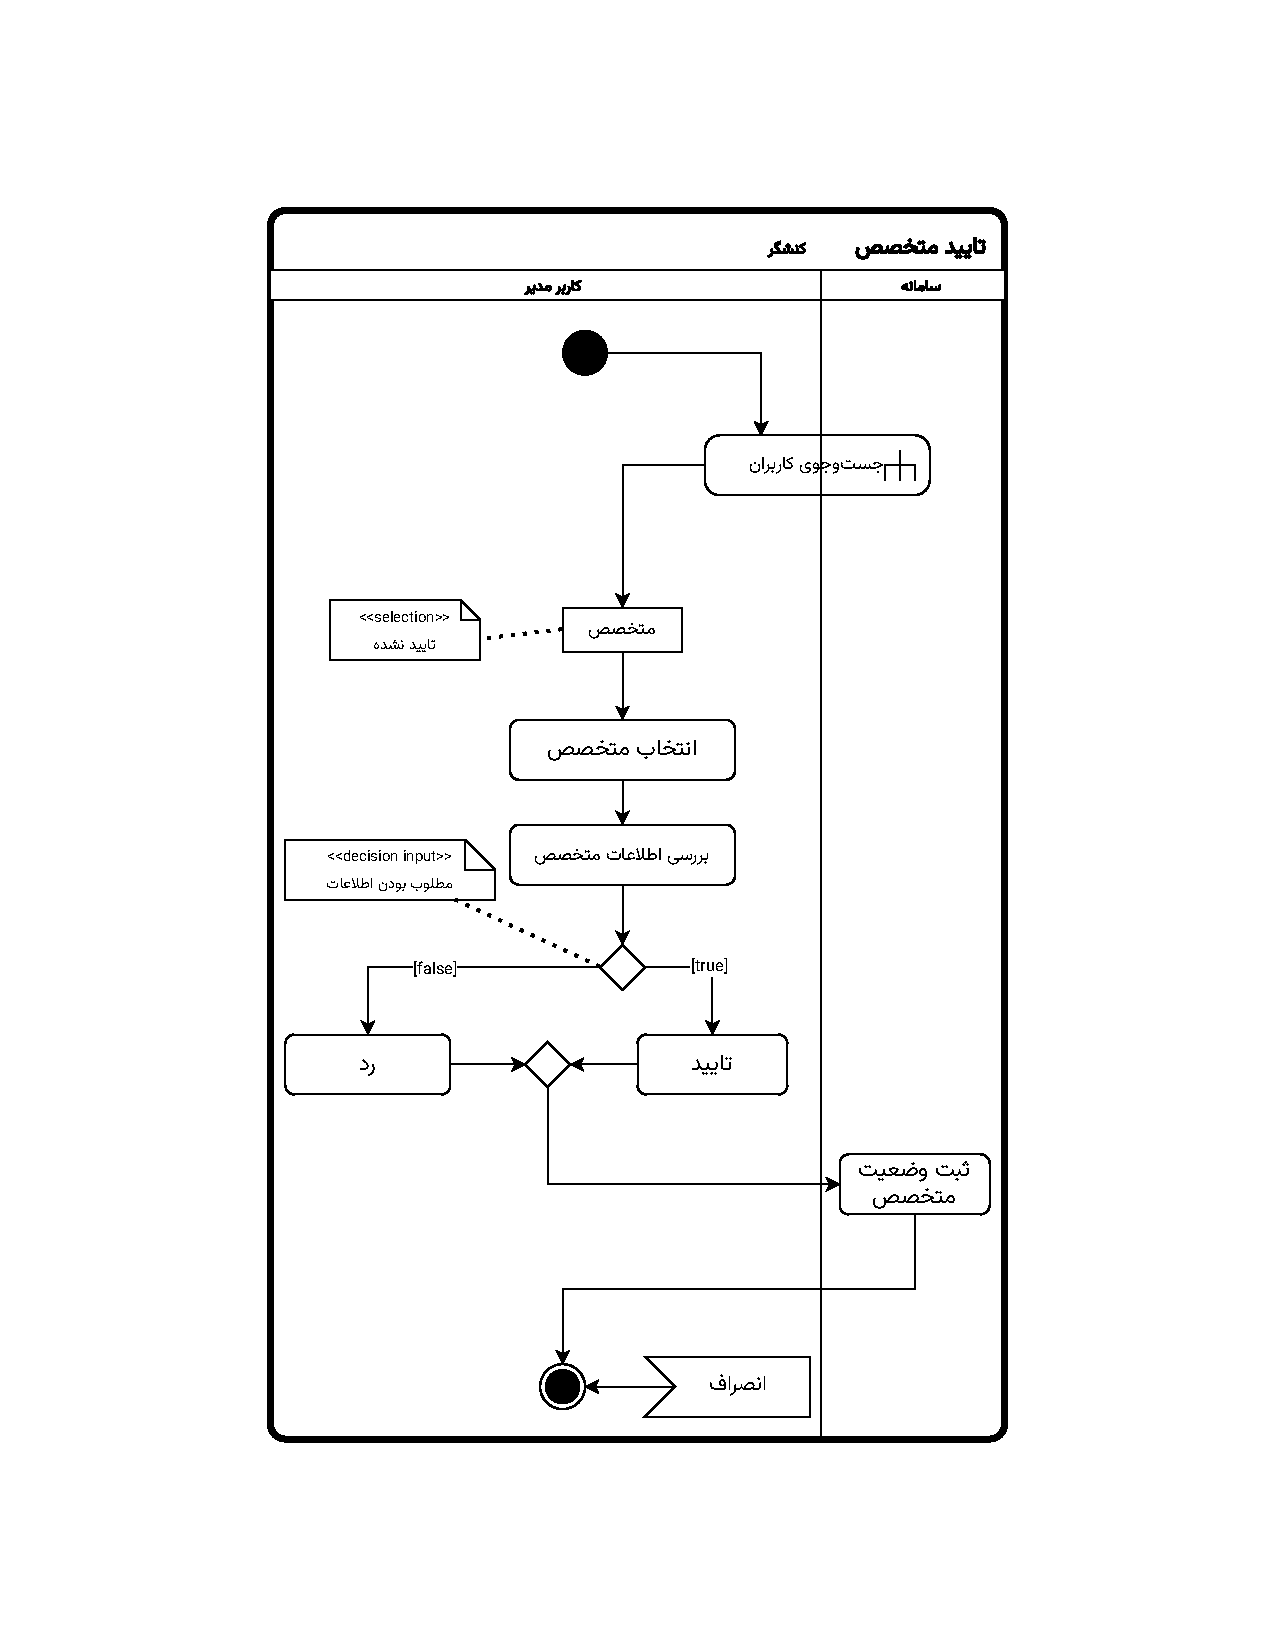
\includegraphics[scale=0.8, page=1]{figs/OOD-activity-confirmspec.pdf}
	\caption{نمودار فعالیت: تایید متخصص}
\end{figure}
\FloatBarrier
\newpage

\begin{figure}[ht!]
	\centering
	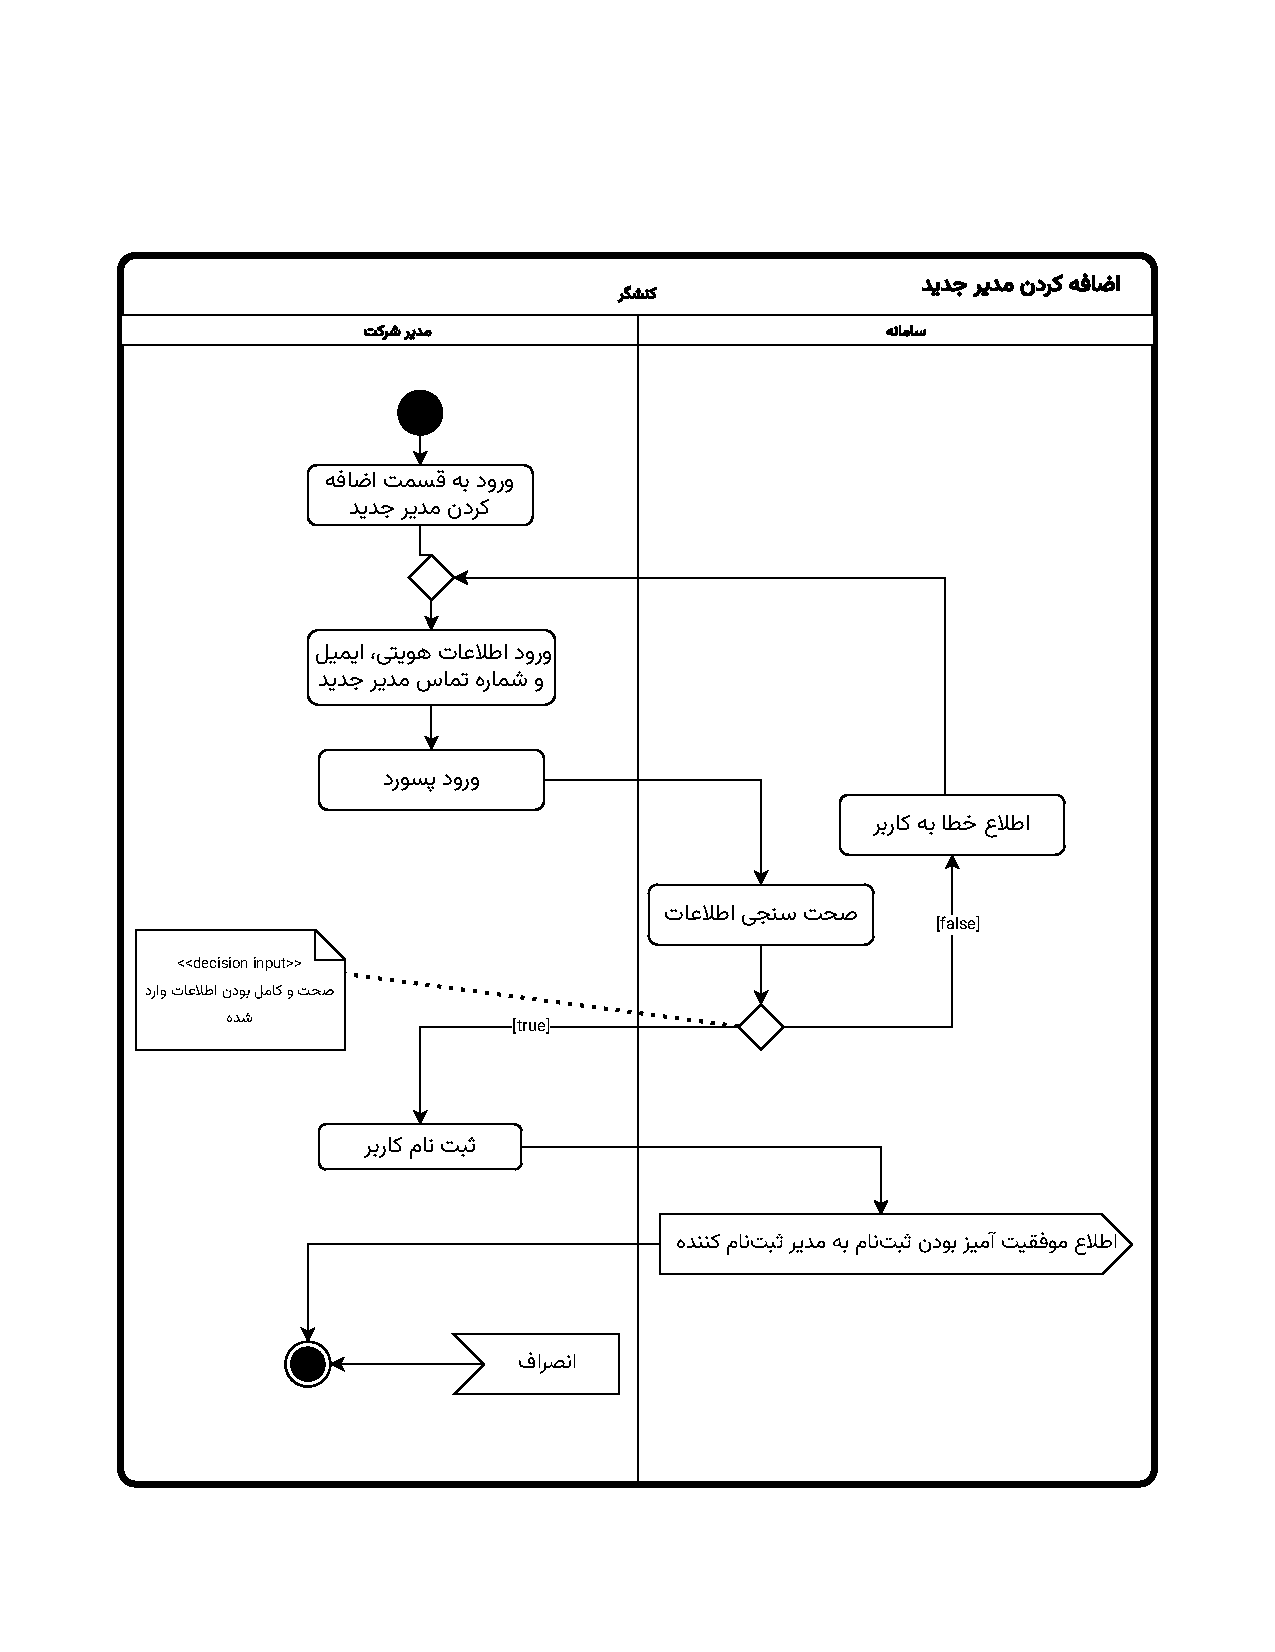
\includegraphics[scale=0.8, page=1]{figs/OOD-activity-addmanager.pdf}
	\caption{نمودار فعالیت: اضافه کردن مدیر جدید}
\end{figure}
\FloatBarrier
\newpage

\begin{figure}[ht!]
	\centering
	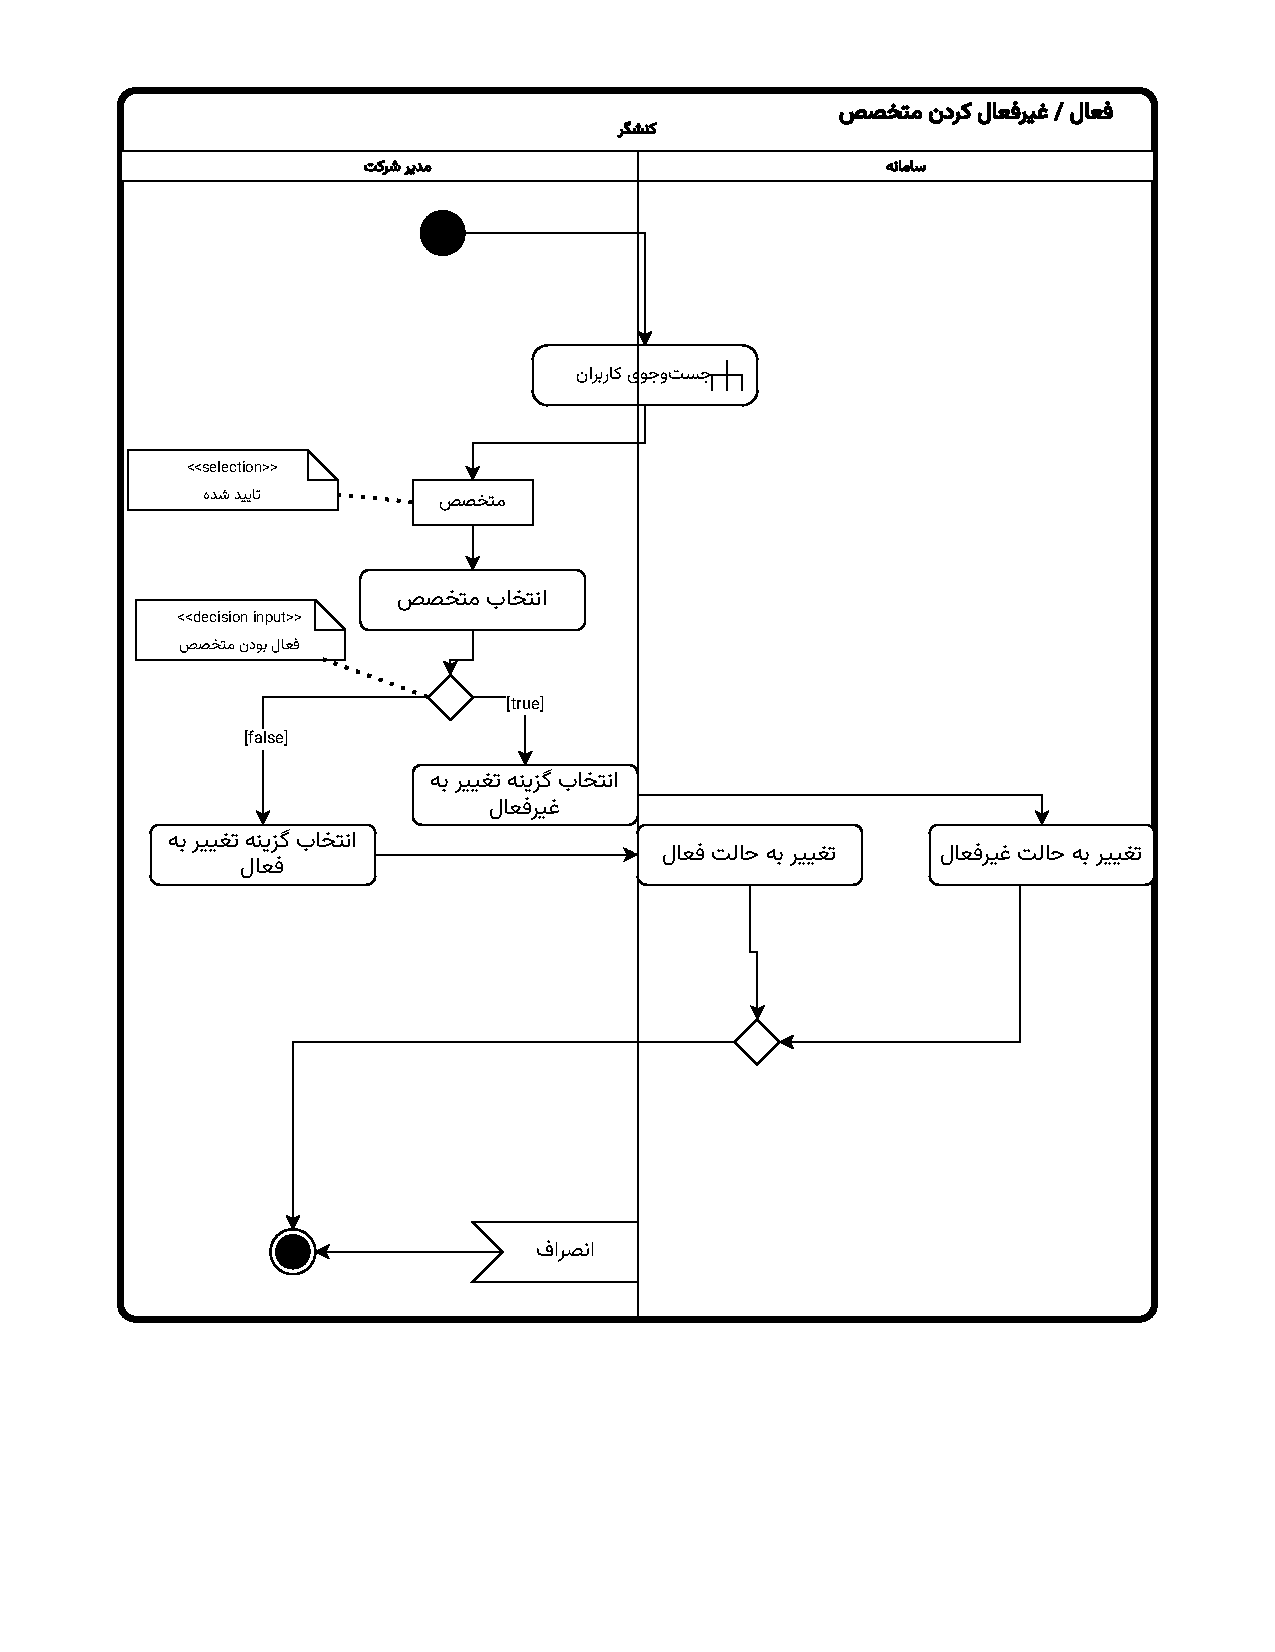
\includegraphics[scale=0.8, page=1]{figs/OOD-activity-activedeactive.pdf}
	\caption{نمودار فعالیت: فعال یا غیرفعال کردن متخصص}
\end{figure}
\FloatBarrier
\newpage

\begin{figure}[ht!]
	\centering
	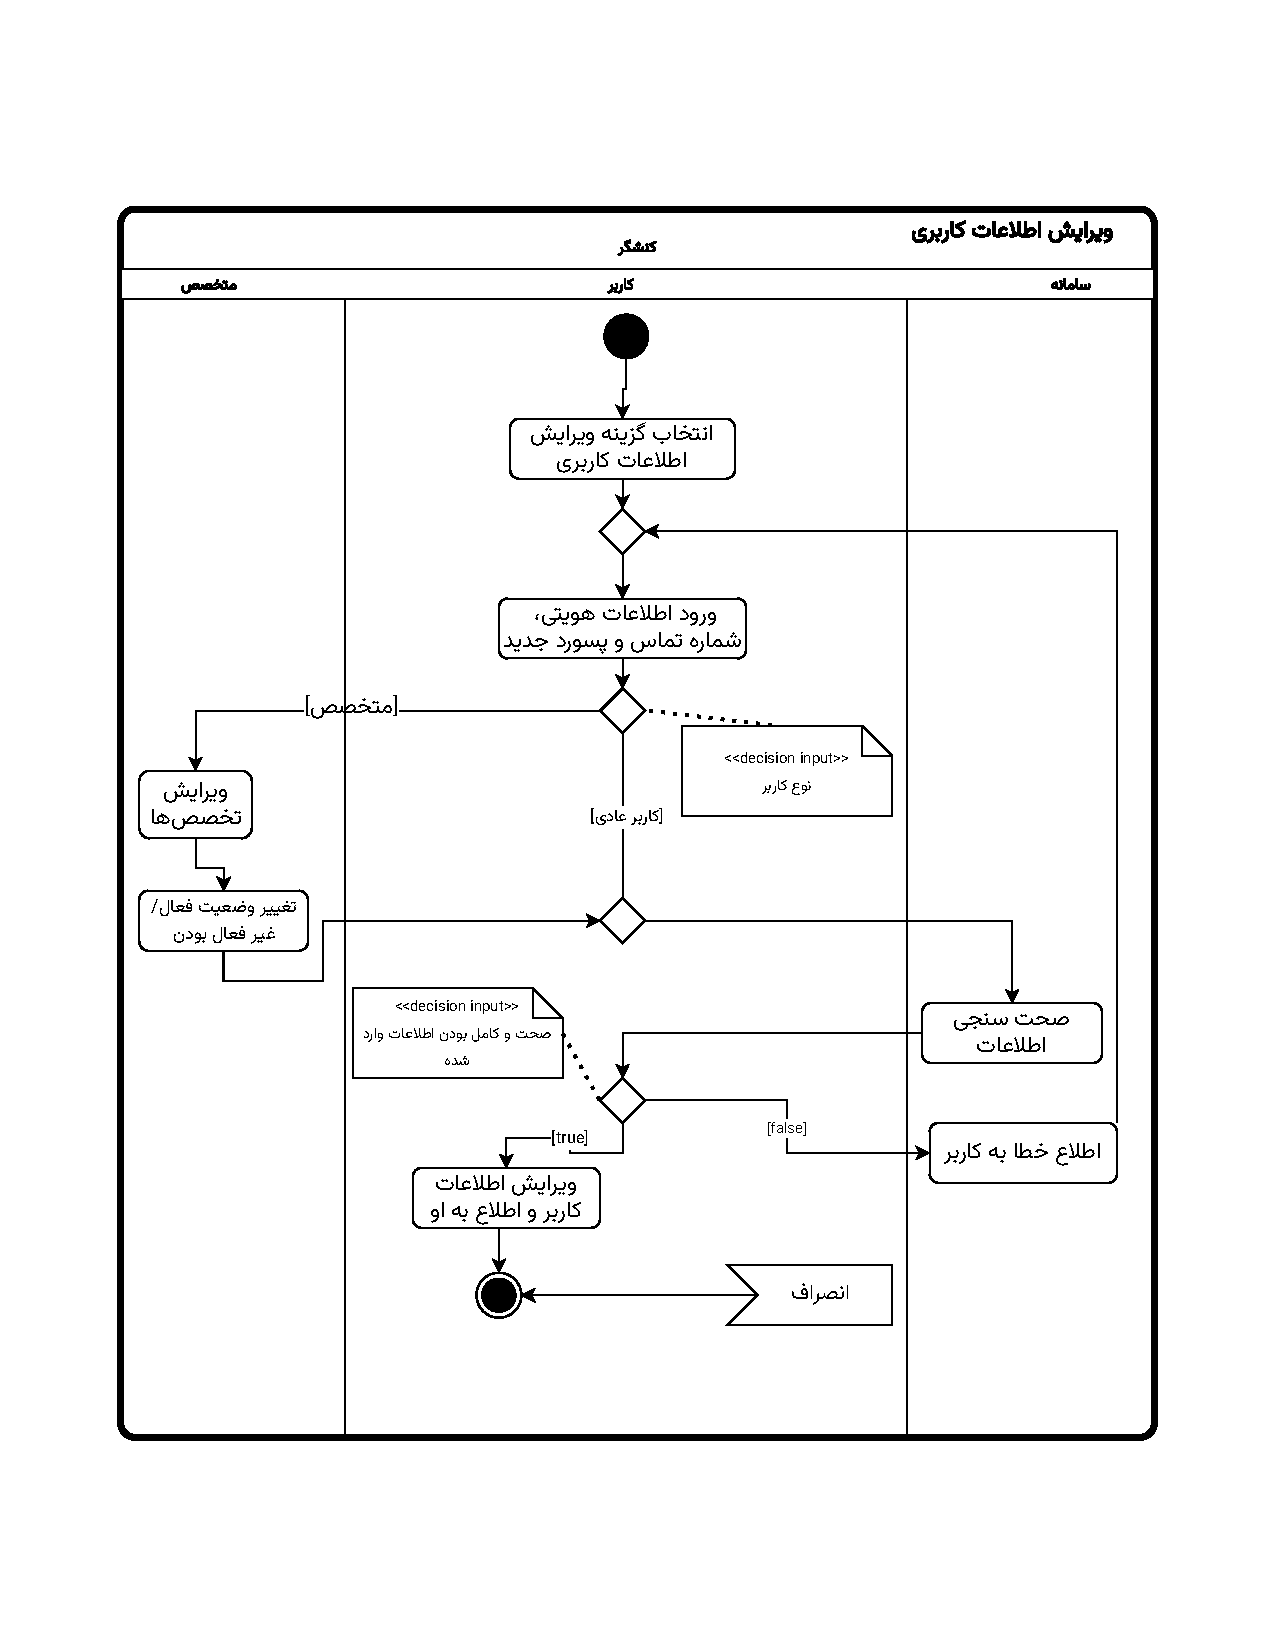
\includegraphics[scale=0.8, page=1]{figs/OOD-activity-edituser.pdf}
	\caption{نمودار فعالیت: ویرایش اطلاعات کاربری}
\end{figure}
\FloatBarrier
\newpage


\section{زیرسیستم خدمت‌دهی}


\begin{figure}[ht!]
	\centering
	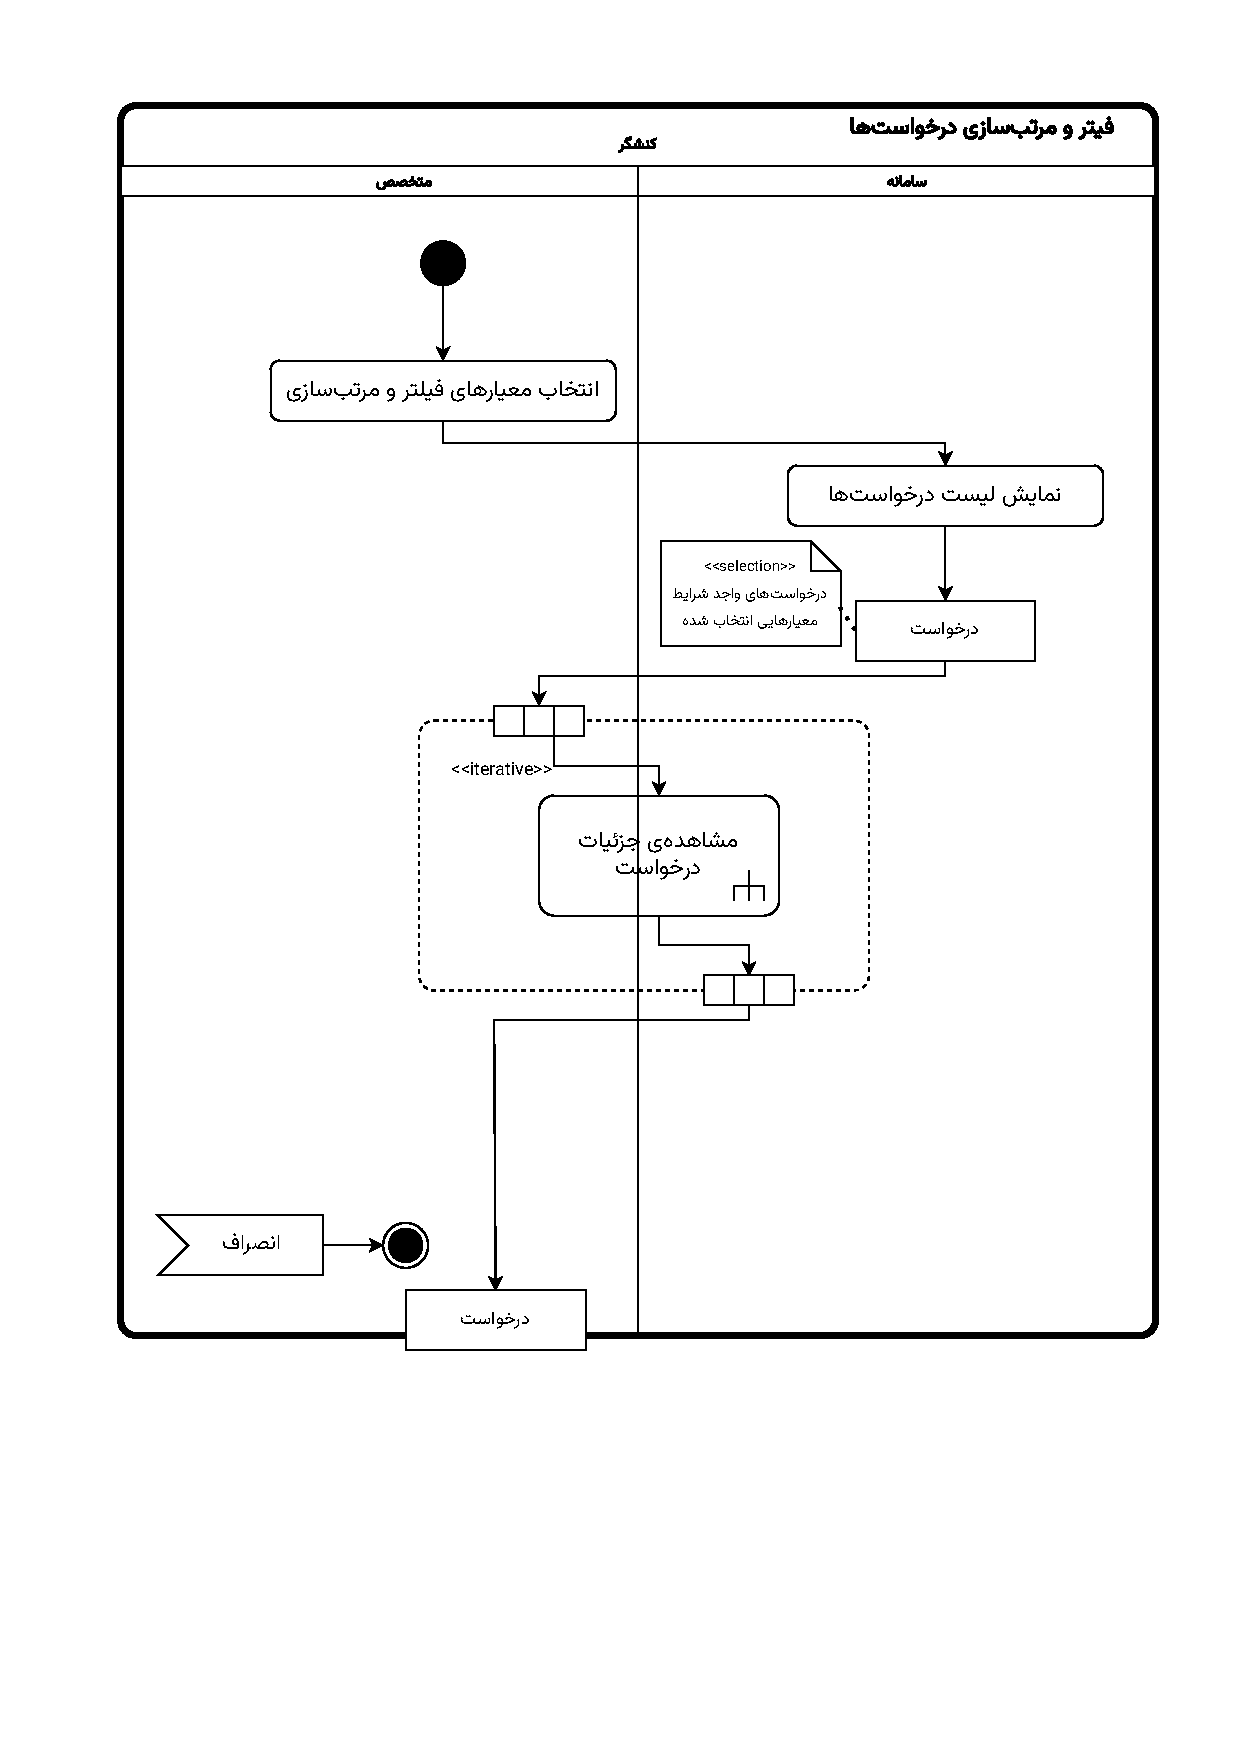
\includegraphics[scale=0.6, page=1]{figs/OOD-activity-filterreq.pdf}
	\caption{نمودار فعالیت: فیلتر و مرتب‌سازی درخواست‌ها}
\end{figure}
\FloatBarrier
\newpage

\begin{figure}[ht!]
	\centering
	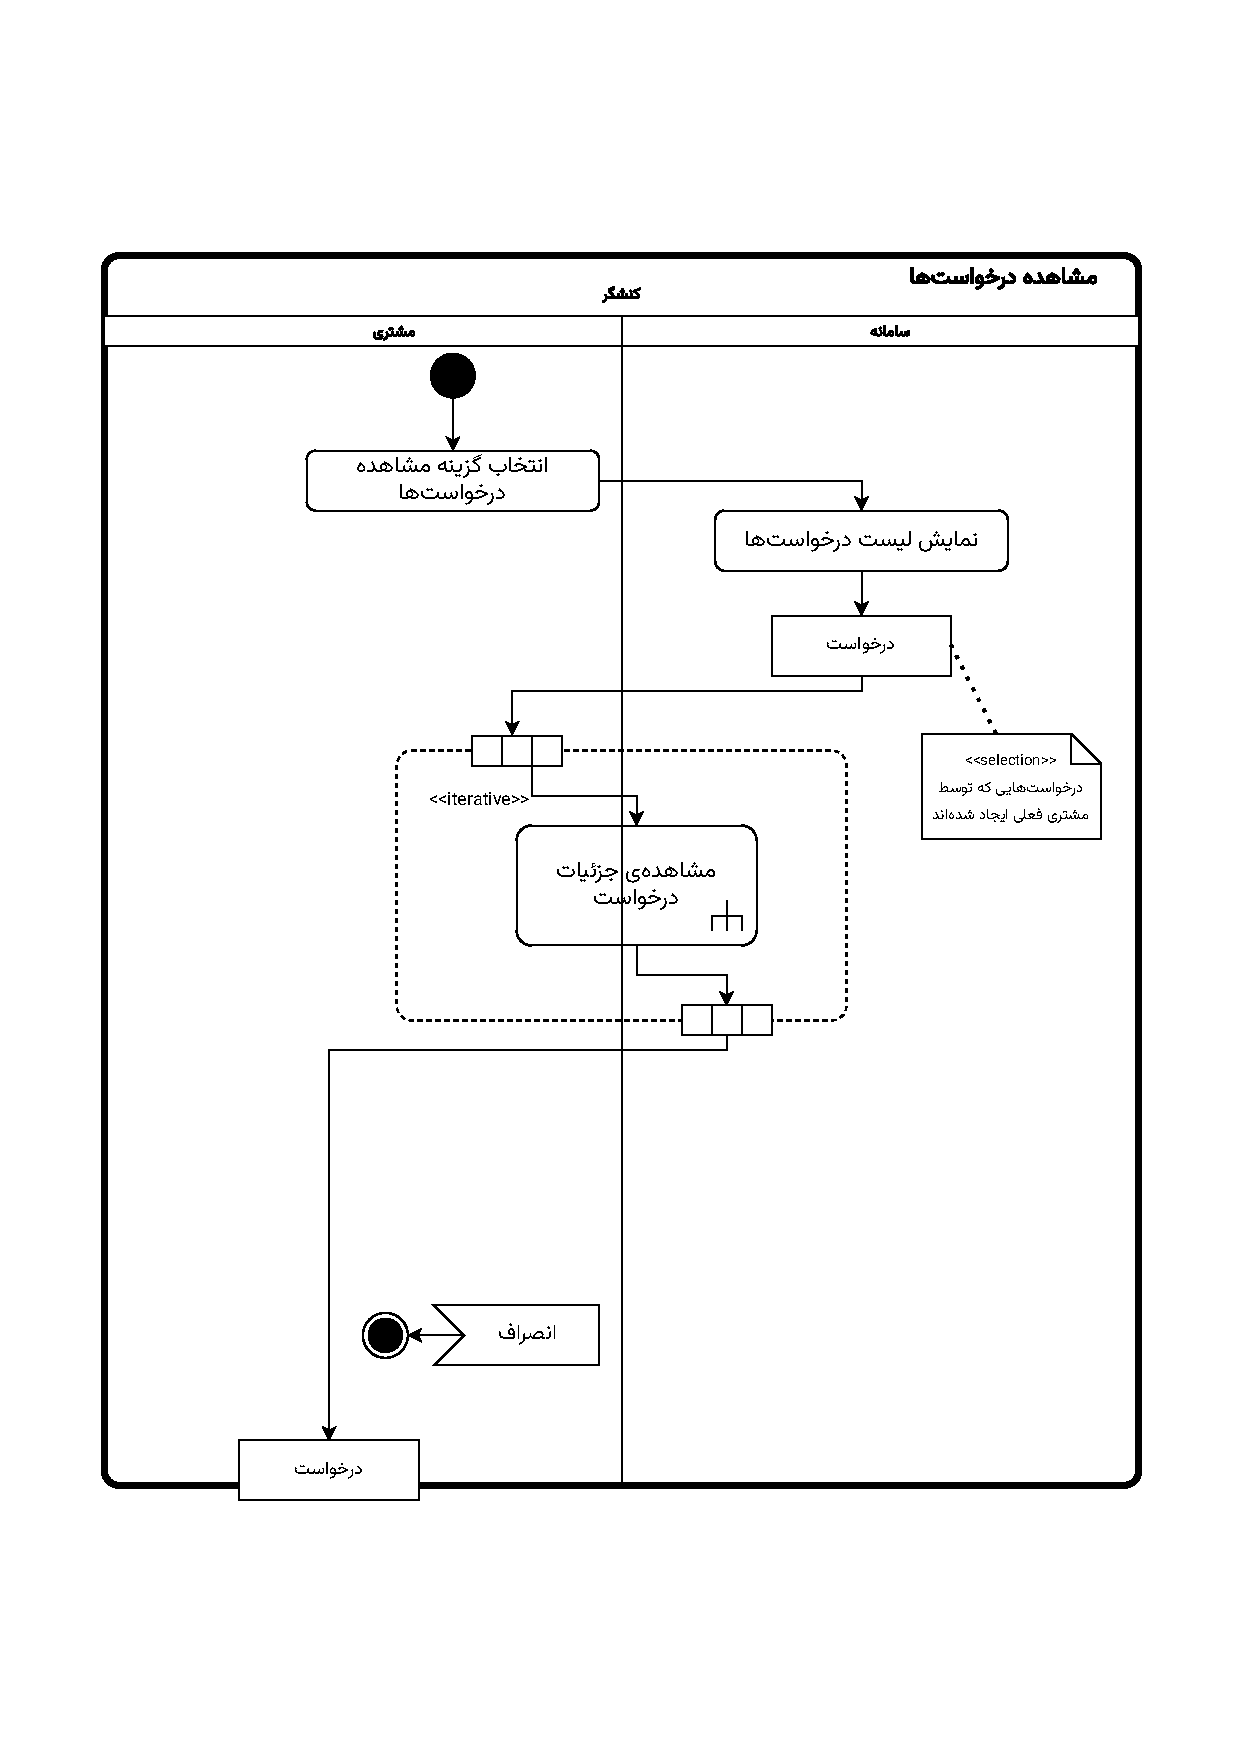
\includegraphics[scale=0.8, page=1]{figs/OOD-activity-viewreq.pdf}
	\caption{نمودار فعالیت: مشاهده درخواست‌ها}
\end{figure}
\FloatBarrier
\newpage

\begin{figure}[ht!]
	\centering
	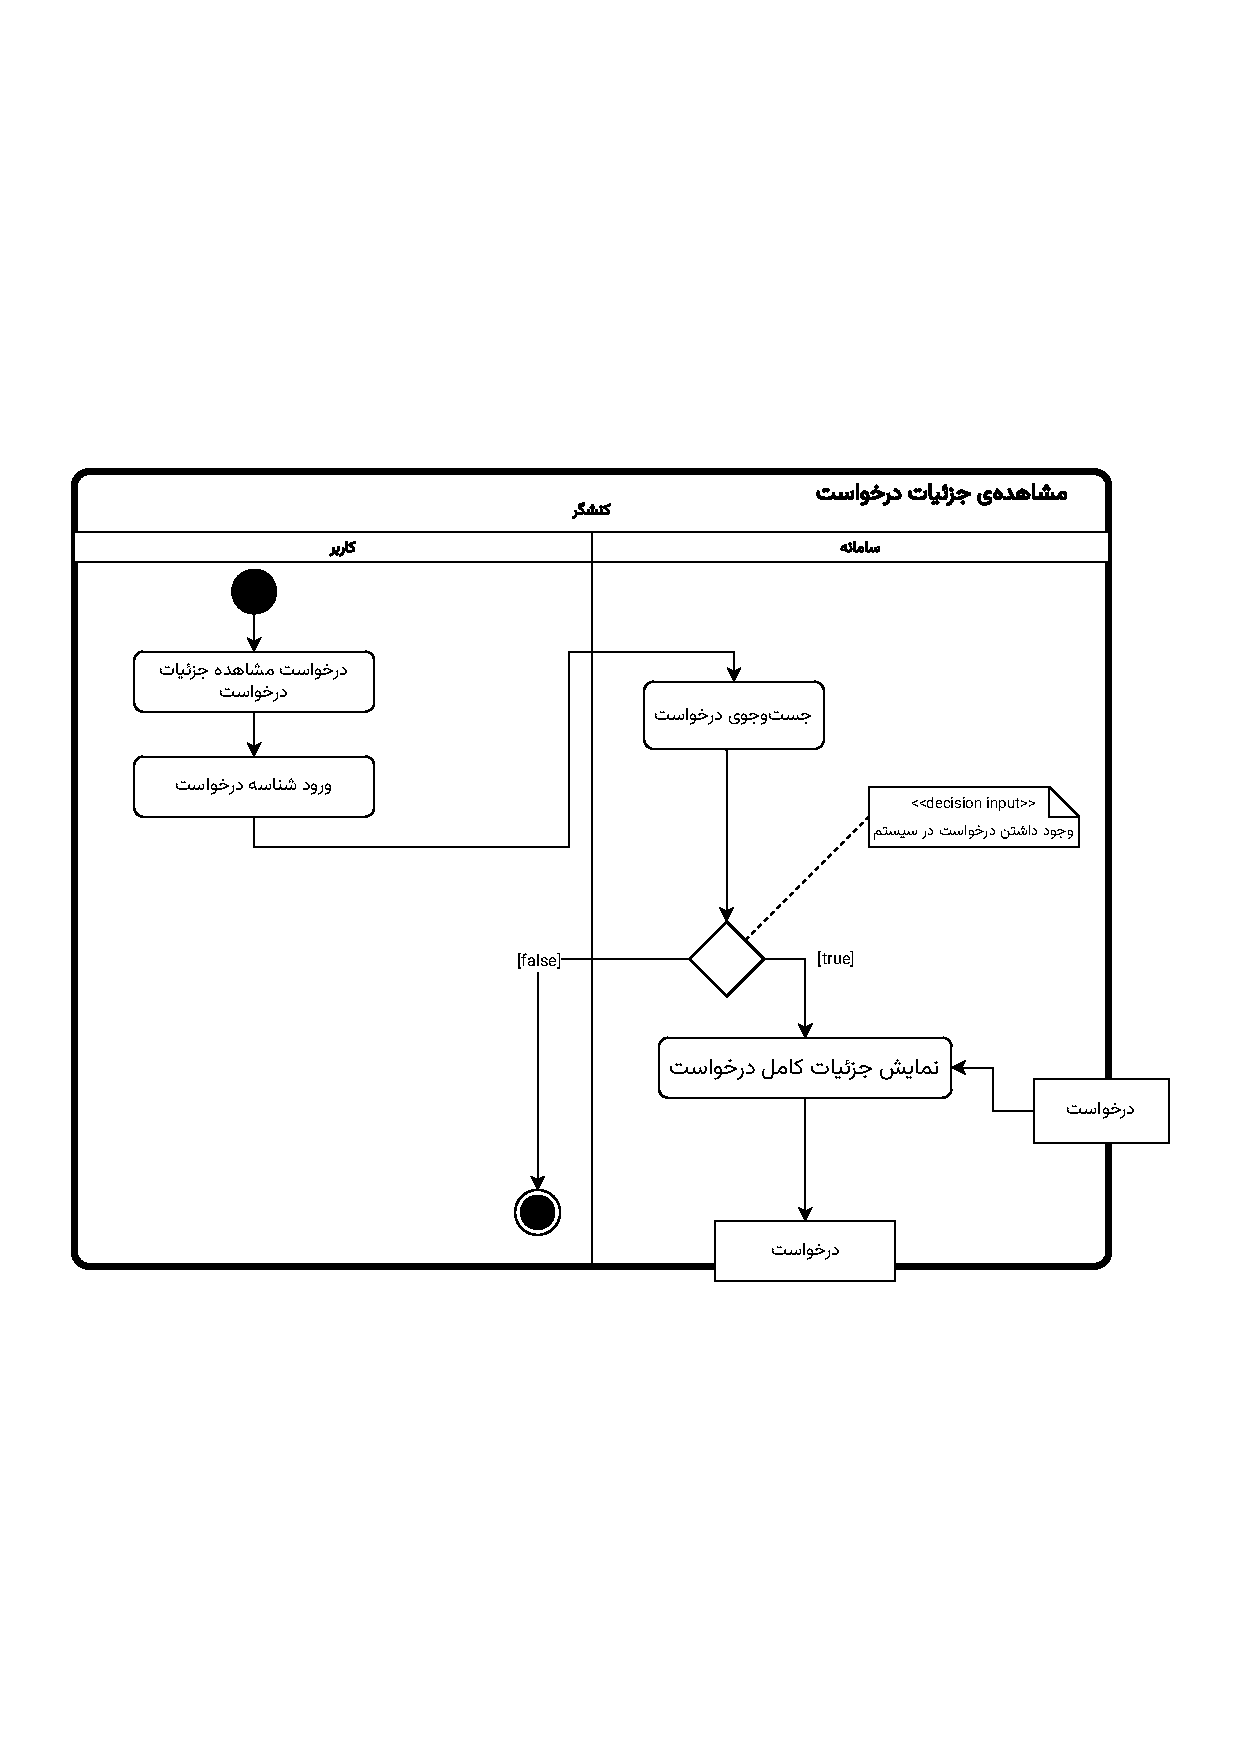
\includegraphics[scale=0.8, page=1]{figs/OOD-activity-detailreq.pdf}
	\caption{نمودار فعالیت: مشاهده جزئیات درخواست}
\end{figure}
\FloatBarrier
\newpage

\begin{figure}[ht!]
	\centering
	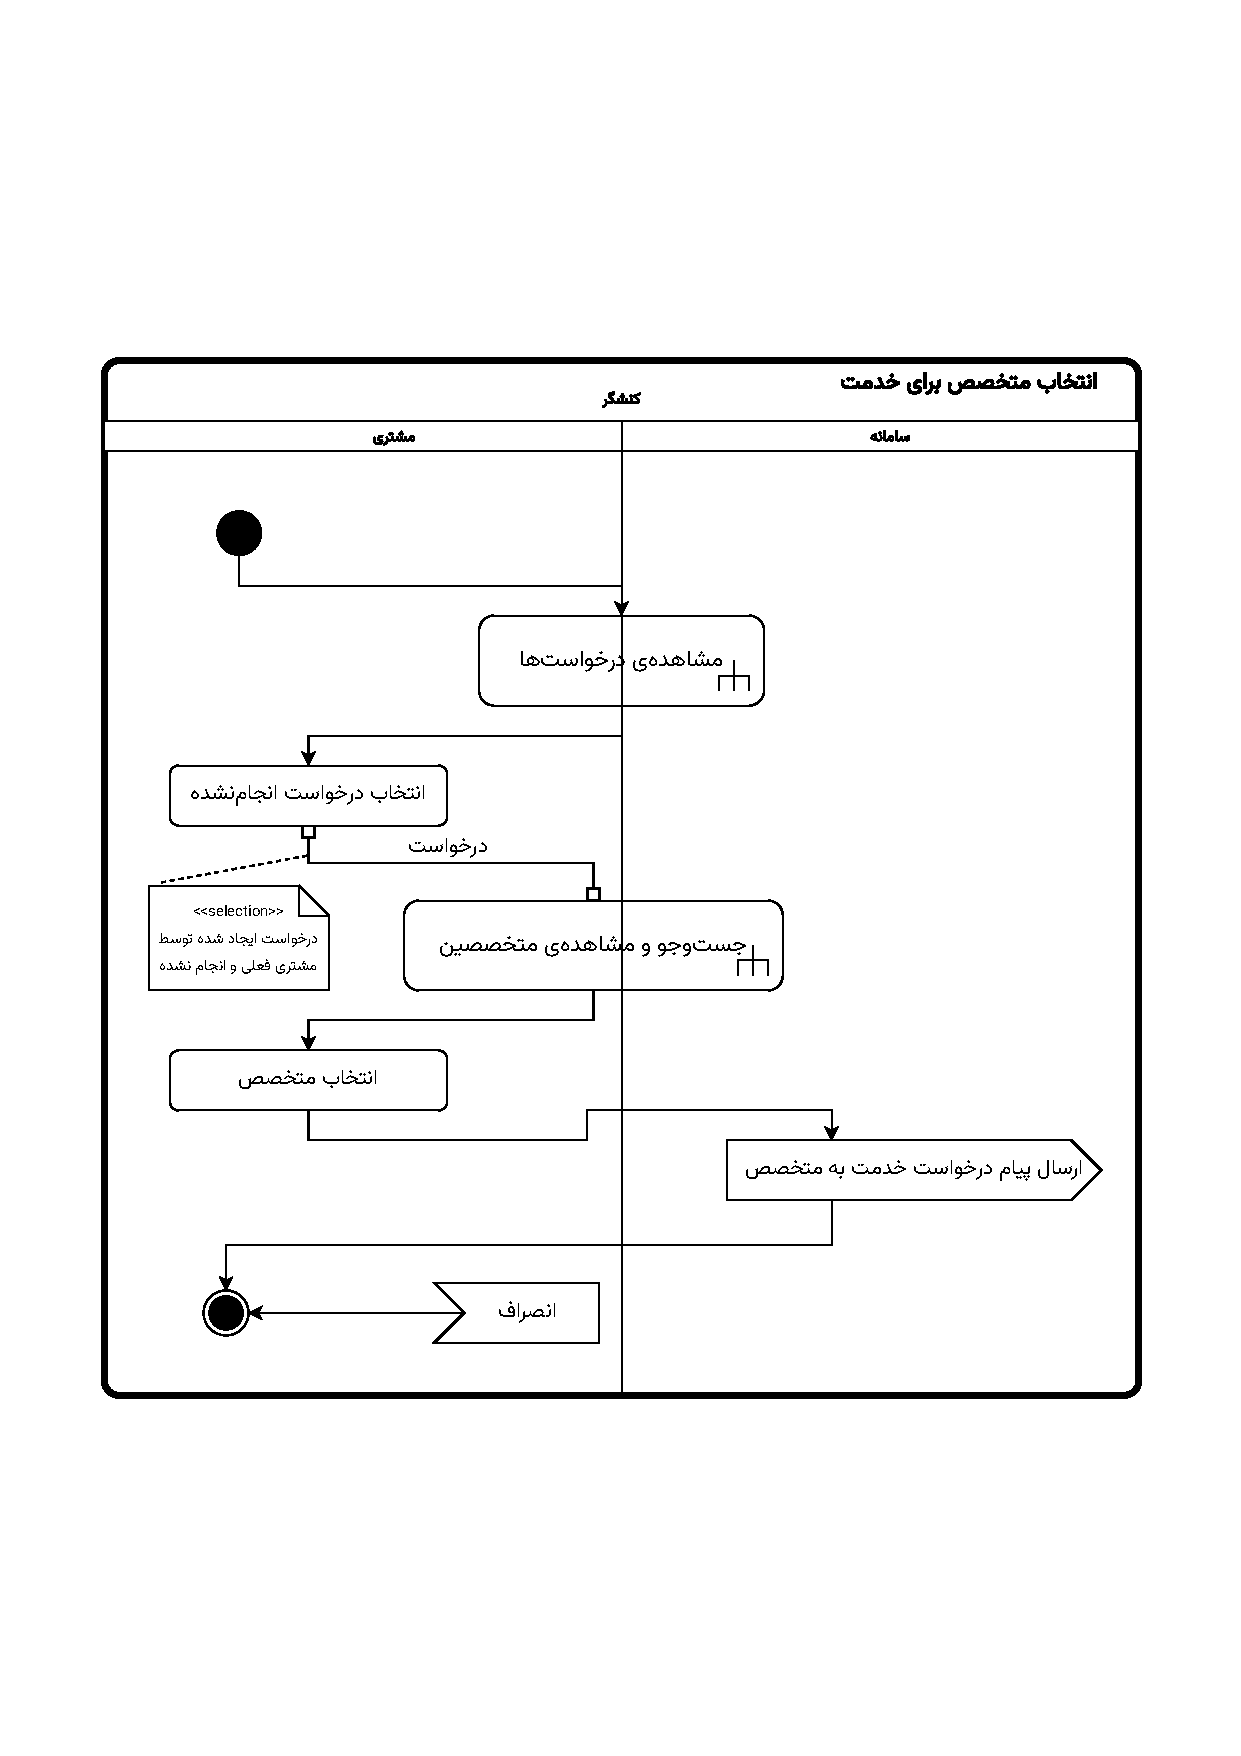
\includegraphics[scale=0.8, page=1]{figs/OOD-activity-selectspecreq.pdf}
	\caption{نمودار فعالیت: انتخاب متخصص برای خدمت}
\end{figure}
\FloatBarrier
\newpage

\begin{figure}[ht!]
	\centering
	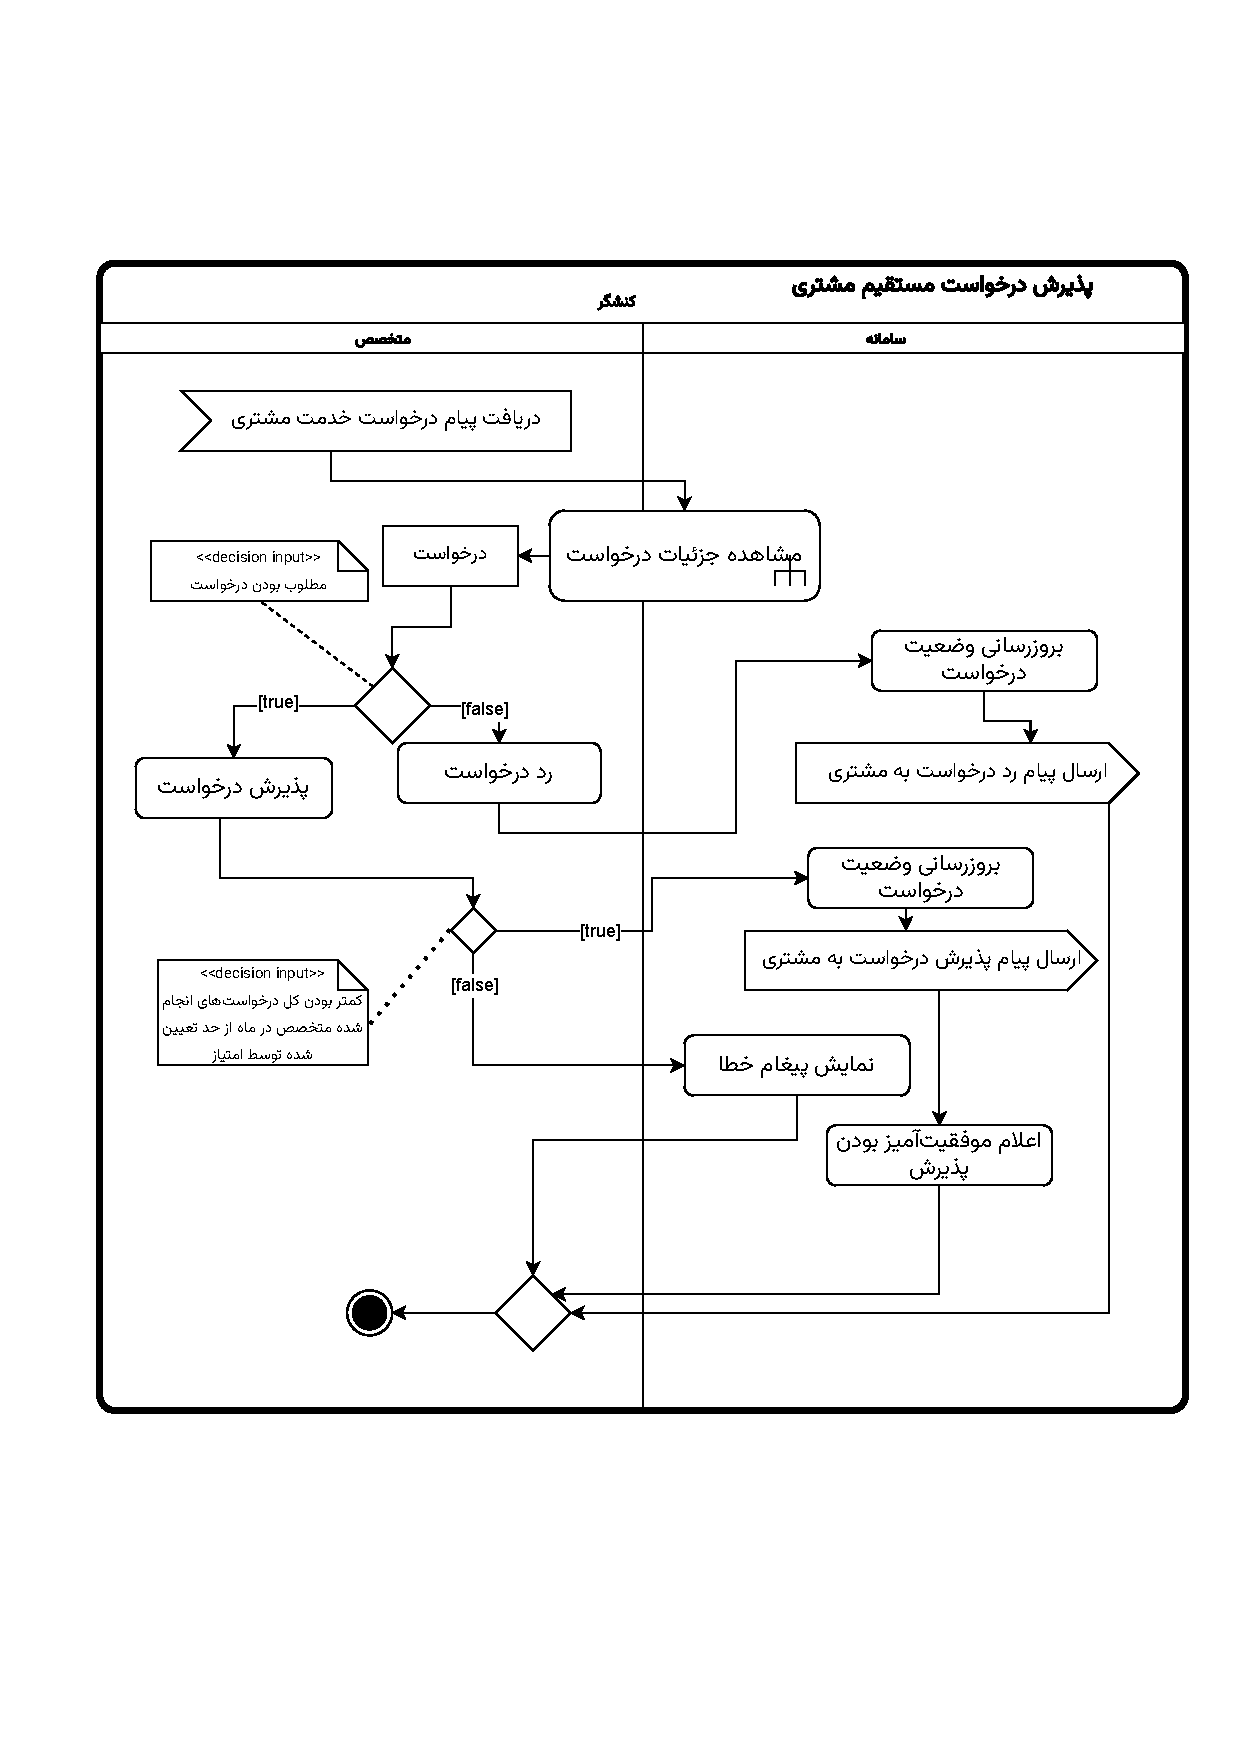
\includegraphics[scale=0.8, page=1]{figs/OOD-activity-directaccept.pdf}
	\caption{نمودار فعالیت: پذیرش درخواست مستقیم مشتری}
\end{figure}
\FloatBarrier
\newpage

\begin{figure}[ht!]
	\centering
	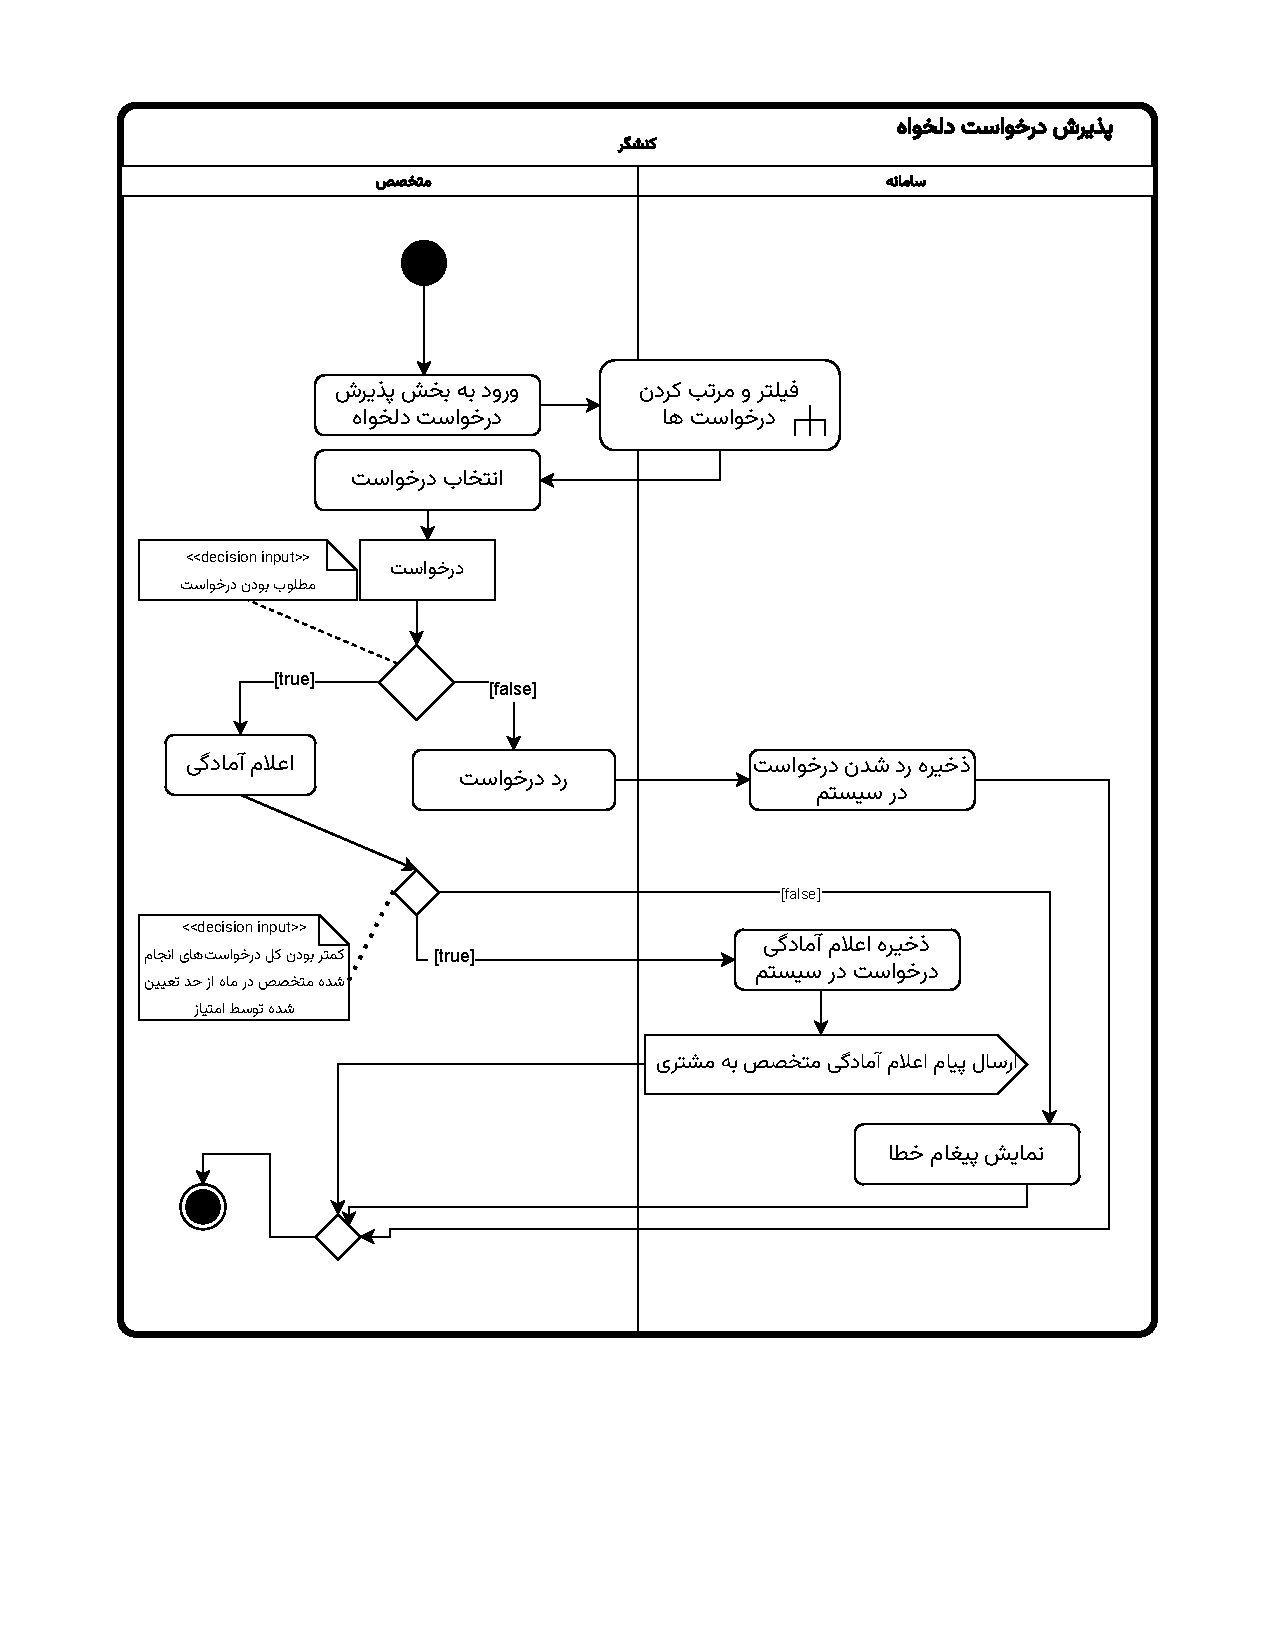
\includegraphics[scale=0.8]{figs/OOD-activity-arbitraryreq.pdf}
	\caption{نمودار فعالیت: پذیرش درخواست دلخواه}
\end{figure}
\FloatBarrier
\newpage

\begin{figure}[ht!]
	\centering
	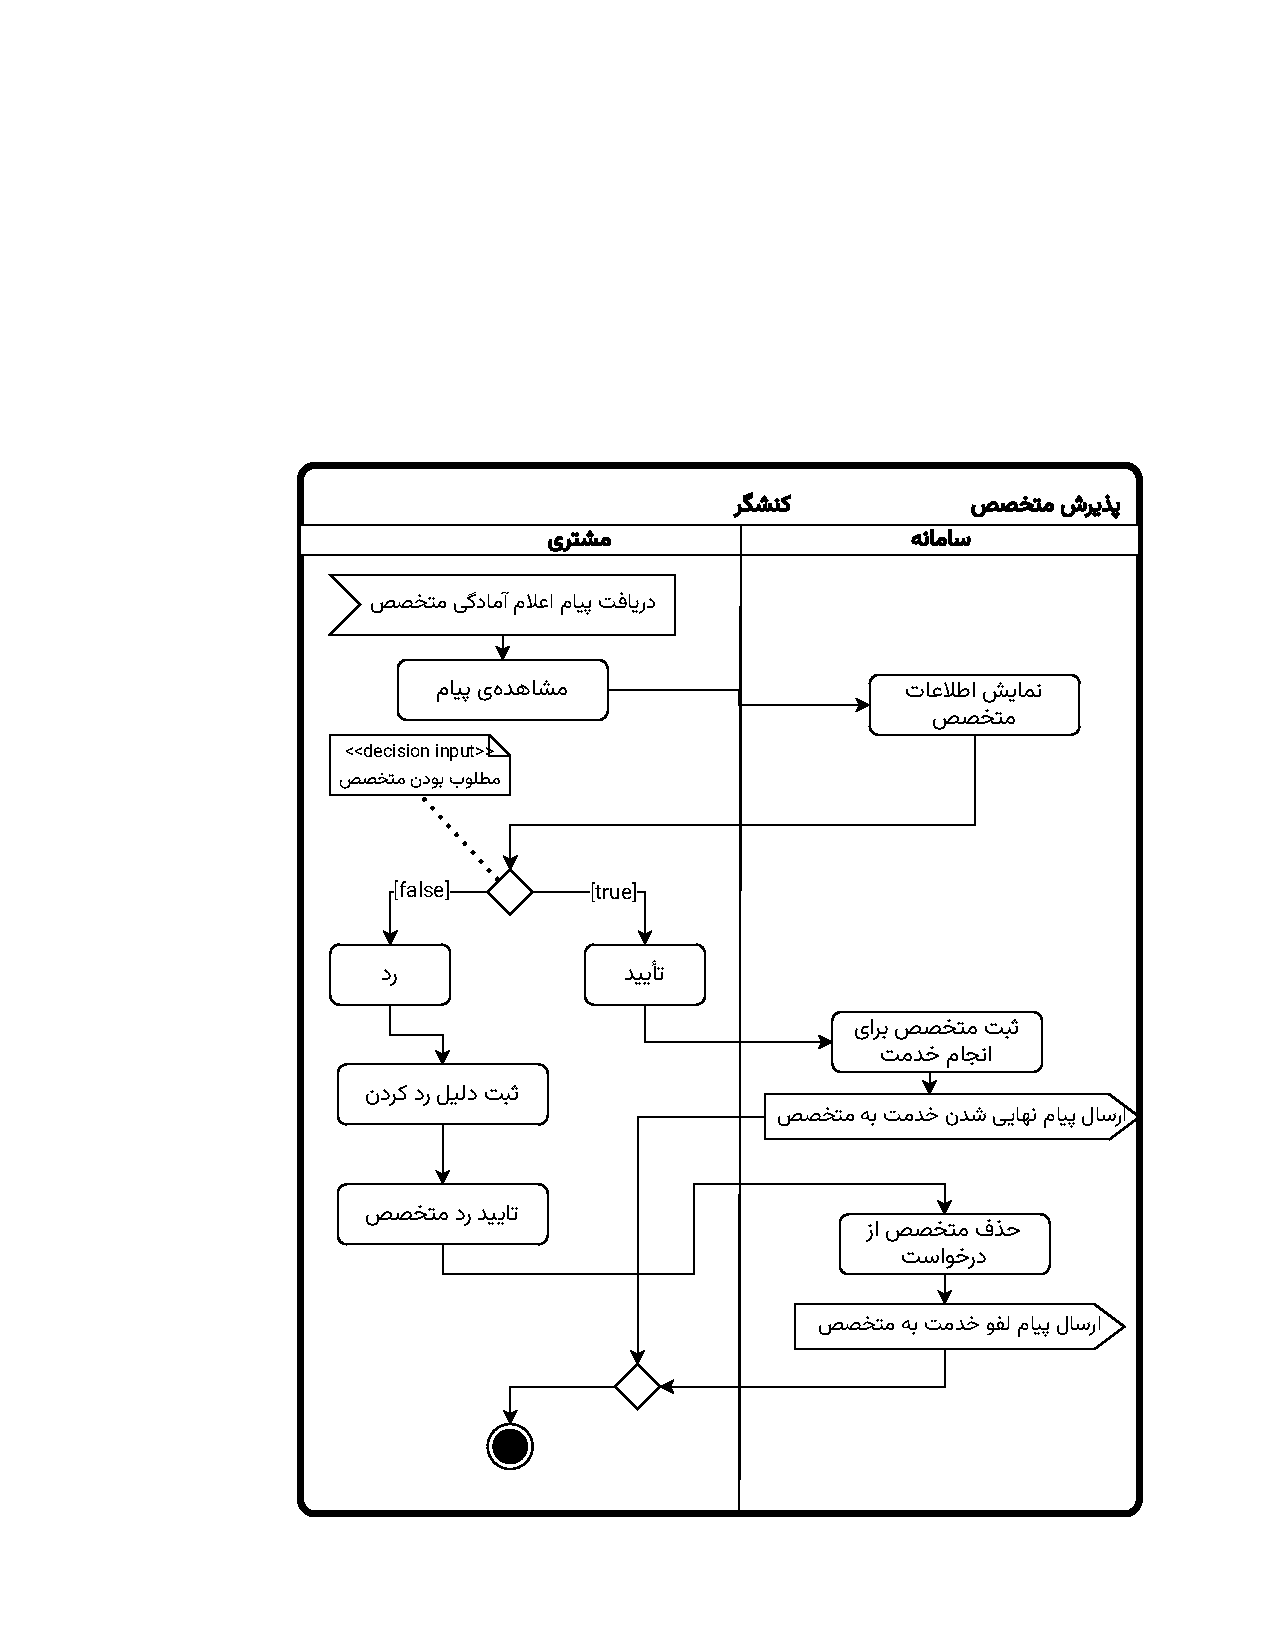
\includegraphics[scale=0.8, page=1]{figs/OOD-activity-acceptspec.pdf}
	\caption{نمودار فعالیت: پذیرش متخصص}
\end{figure}
\FloatBarrier
\newpage

\begin{figure}[ht!]
	\centering
	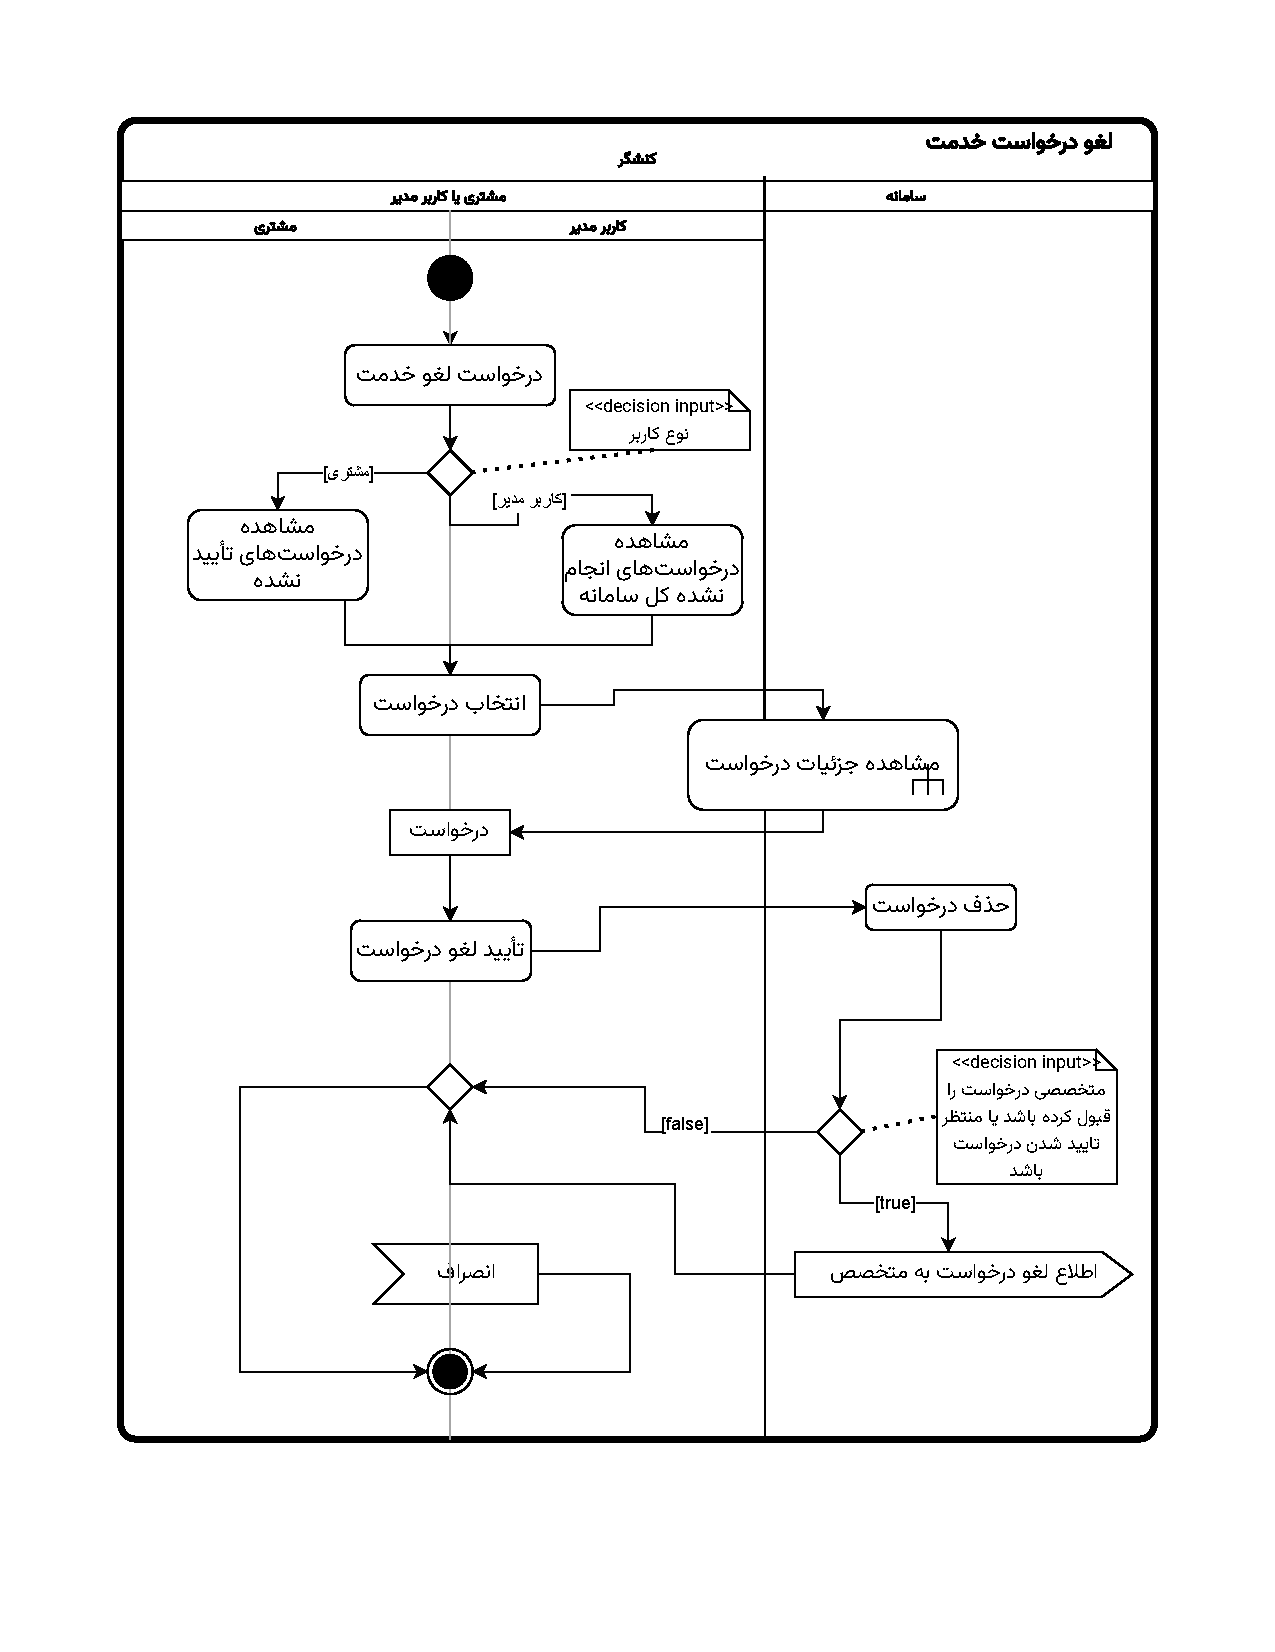
\includegraphics[scale=0.8, page=1]{figs/OOD-activity-cancelreq.pdf}
	\caption{نمودار فعالیت: لغو درخواست خدمت}
\end{figure}
\FloatBarrier
\newpage

\begin{figure}[ht!]
	\centering
	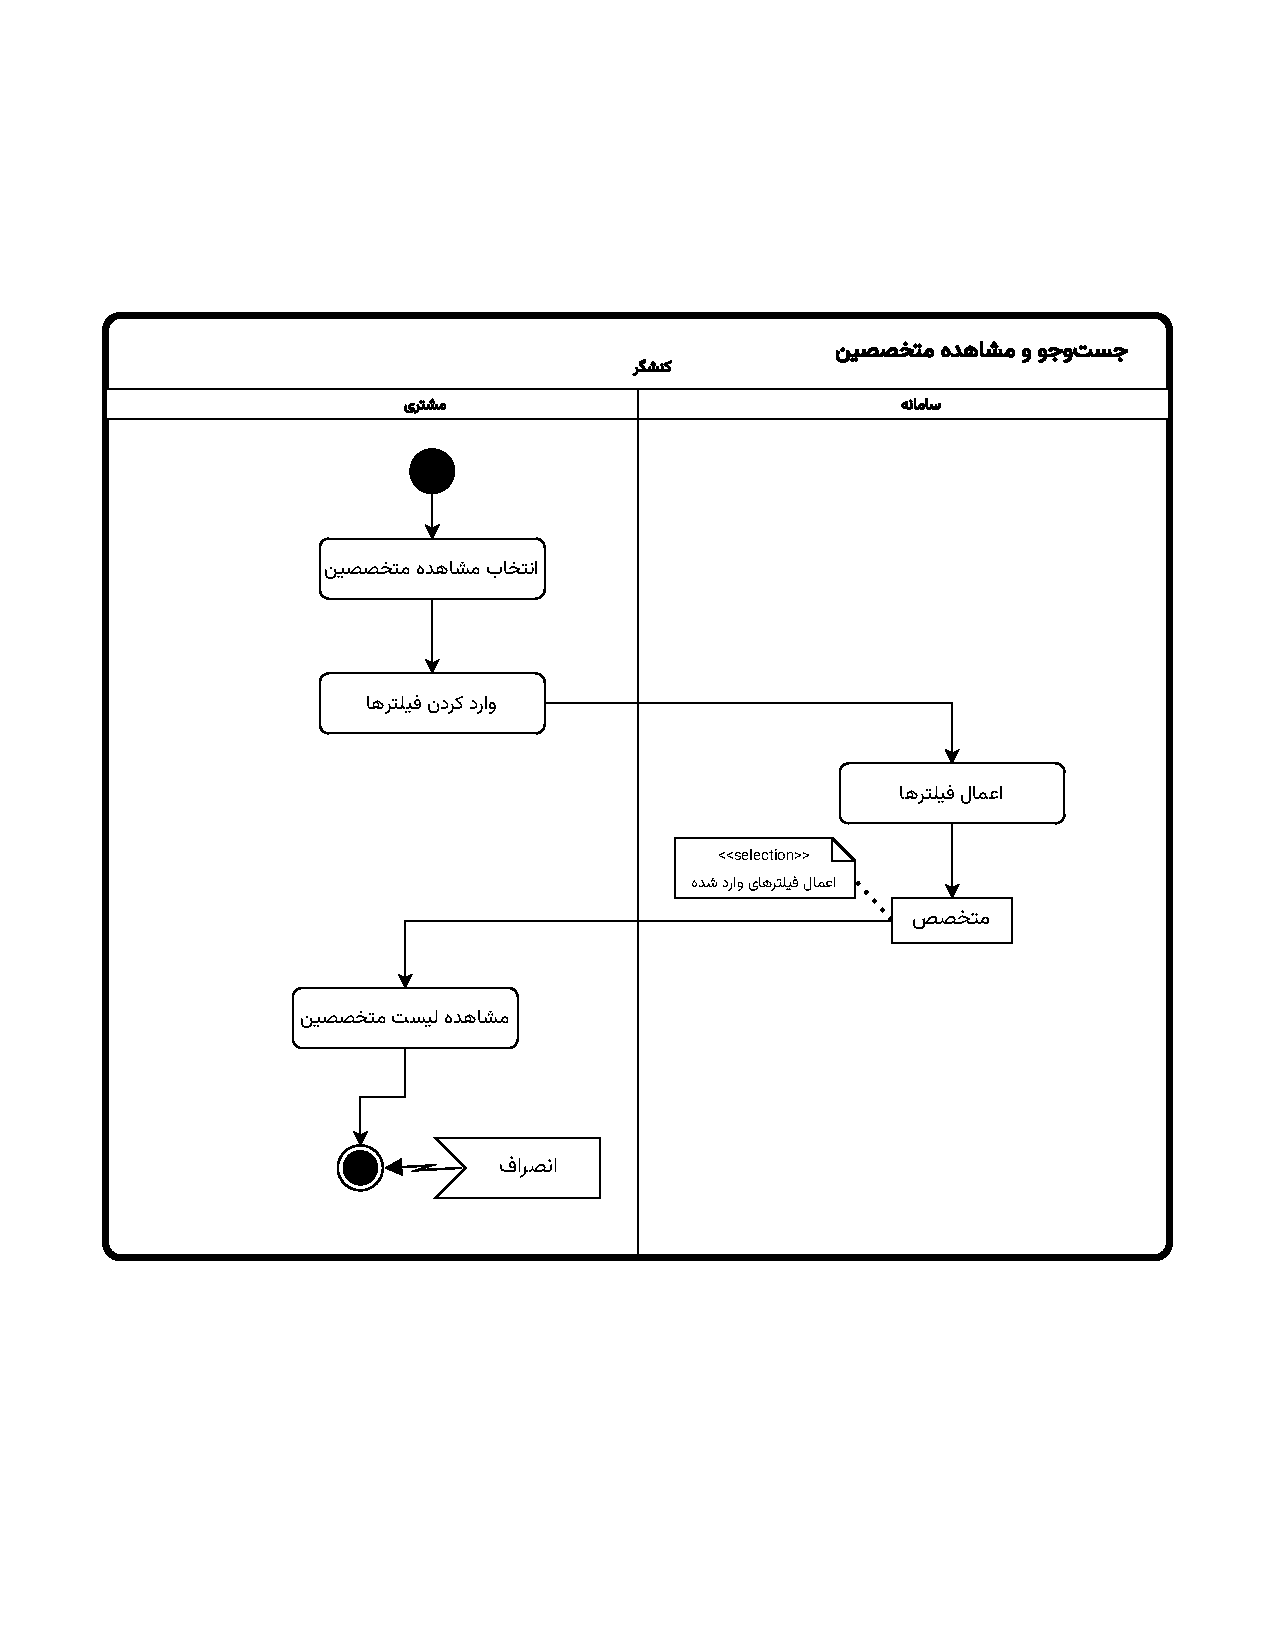
\includegraphics[scale=0.8, page=1]{figs/OOD-activity-searchspec.pdf}
	\caption{نمودار فعالیت: جست‌وجو و مشاهده متخصصین}
\end{figure}
\FloatBarrier
\newpage

\begin{figure}[ht!]
	\centering
	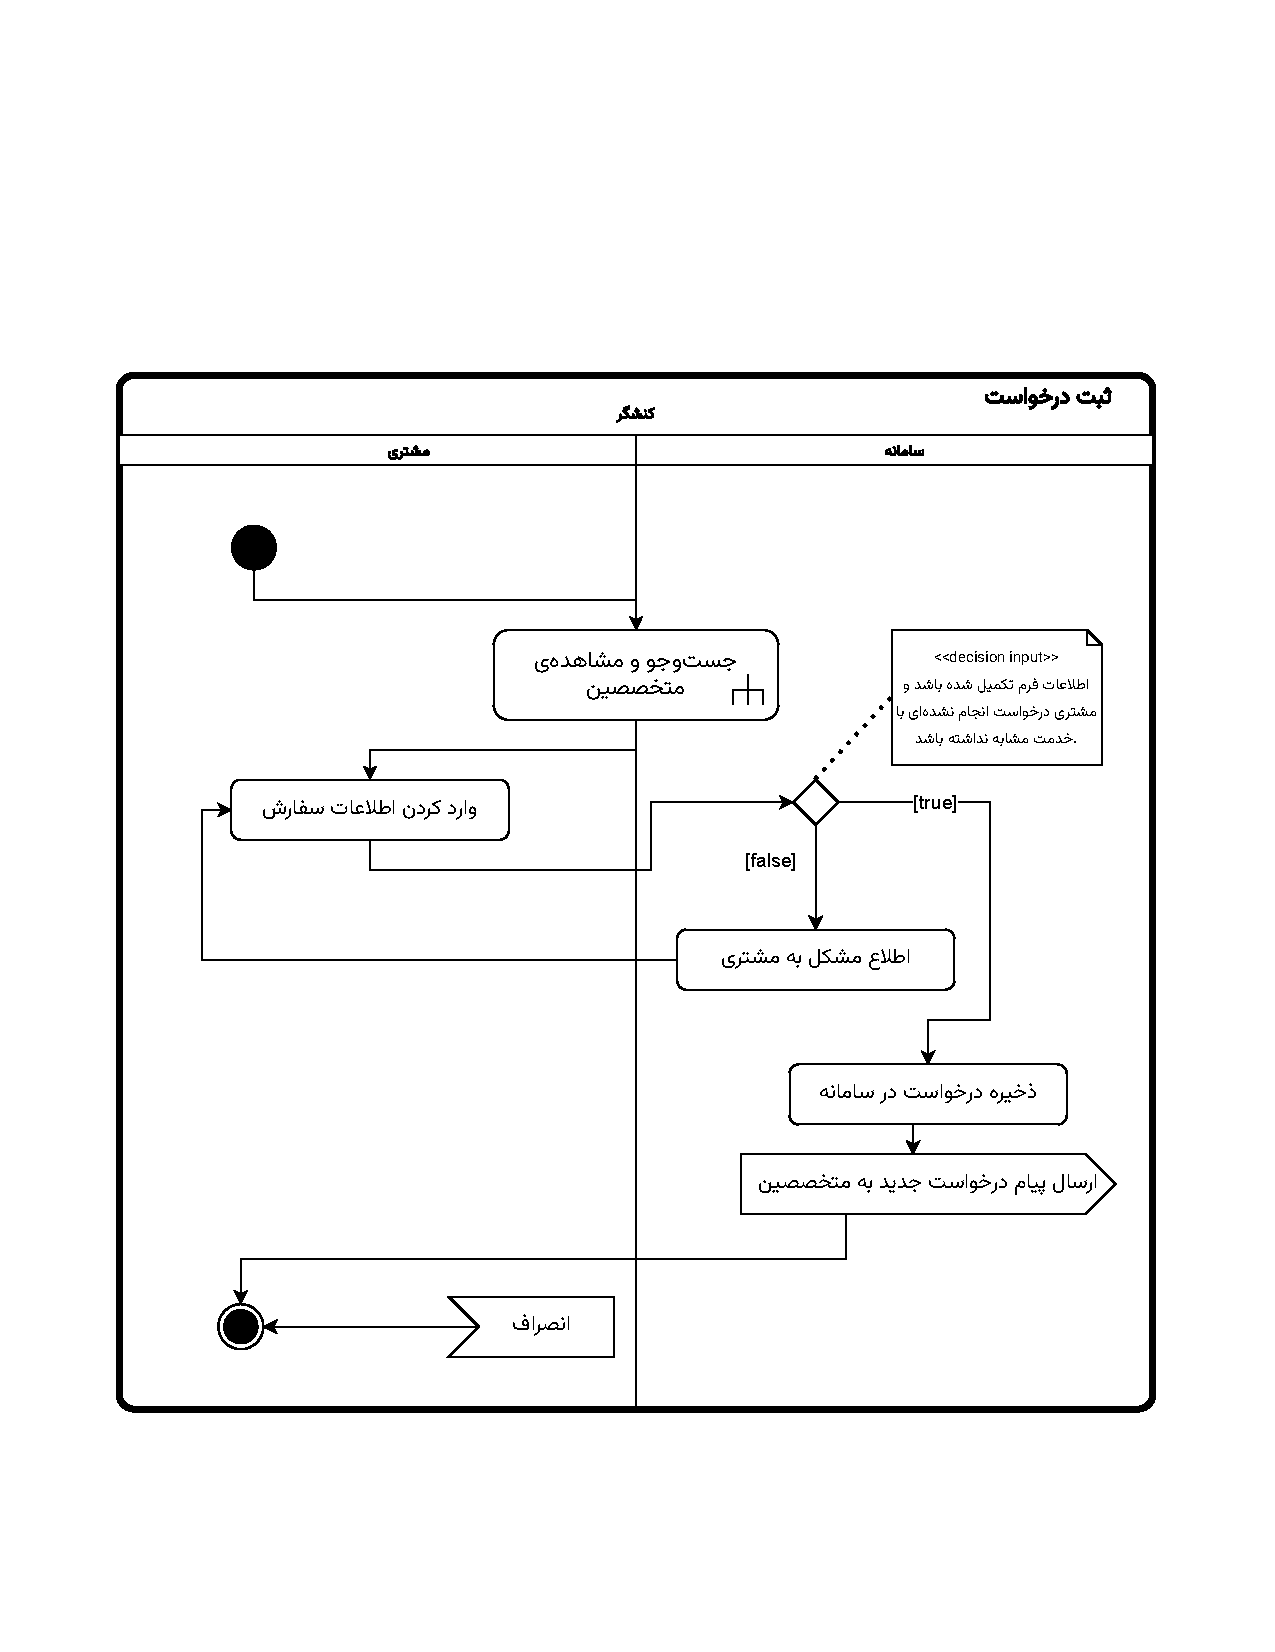
\includegraphics[scale=0.8, page=1]{figs/OOD-activity-submitreq.pdf}
	\caption{نمودار فعالیت: ثبت درخواست}
\end{figure}
\FloatBarrier
\newpage






\begin{figure}[ht!]
	\centering
	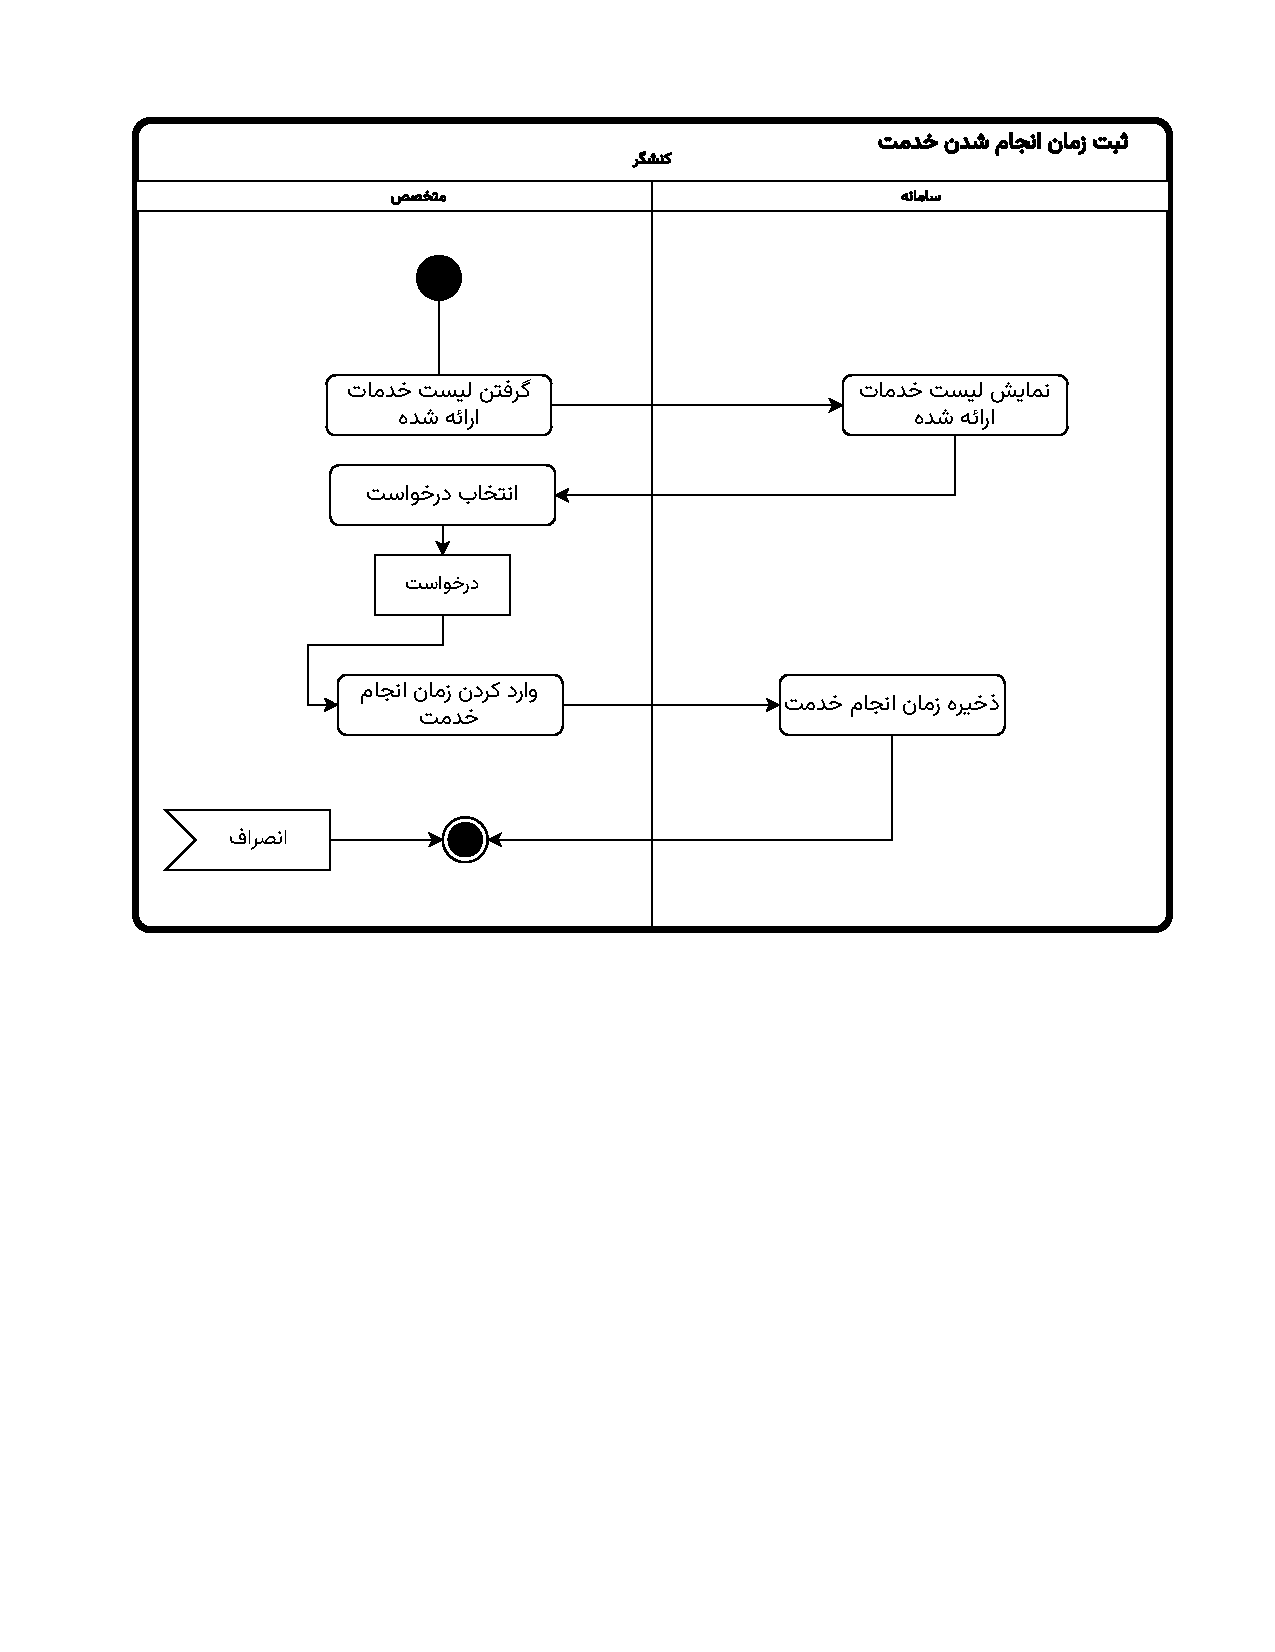
\includegraphics[scale=0.8, page=1]{figs/OOD-activity-reqtime.pdf}
	\caption{نمودار فعالیت: ثبت زمان انجام شدن خدمت}
\end{figure}
\FloatBarrier
\newpage

\begin{figure}[ht!]
	\centering
	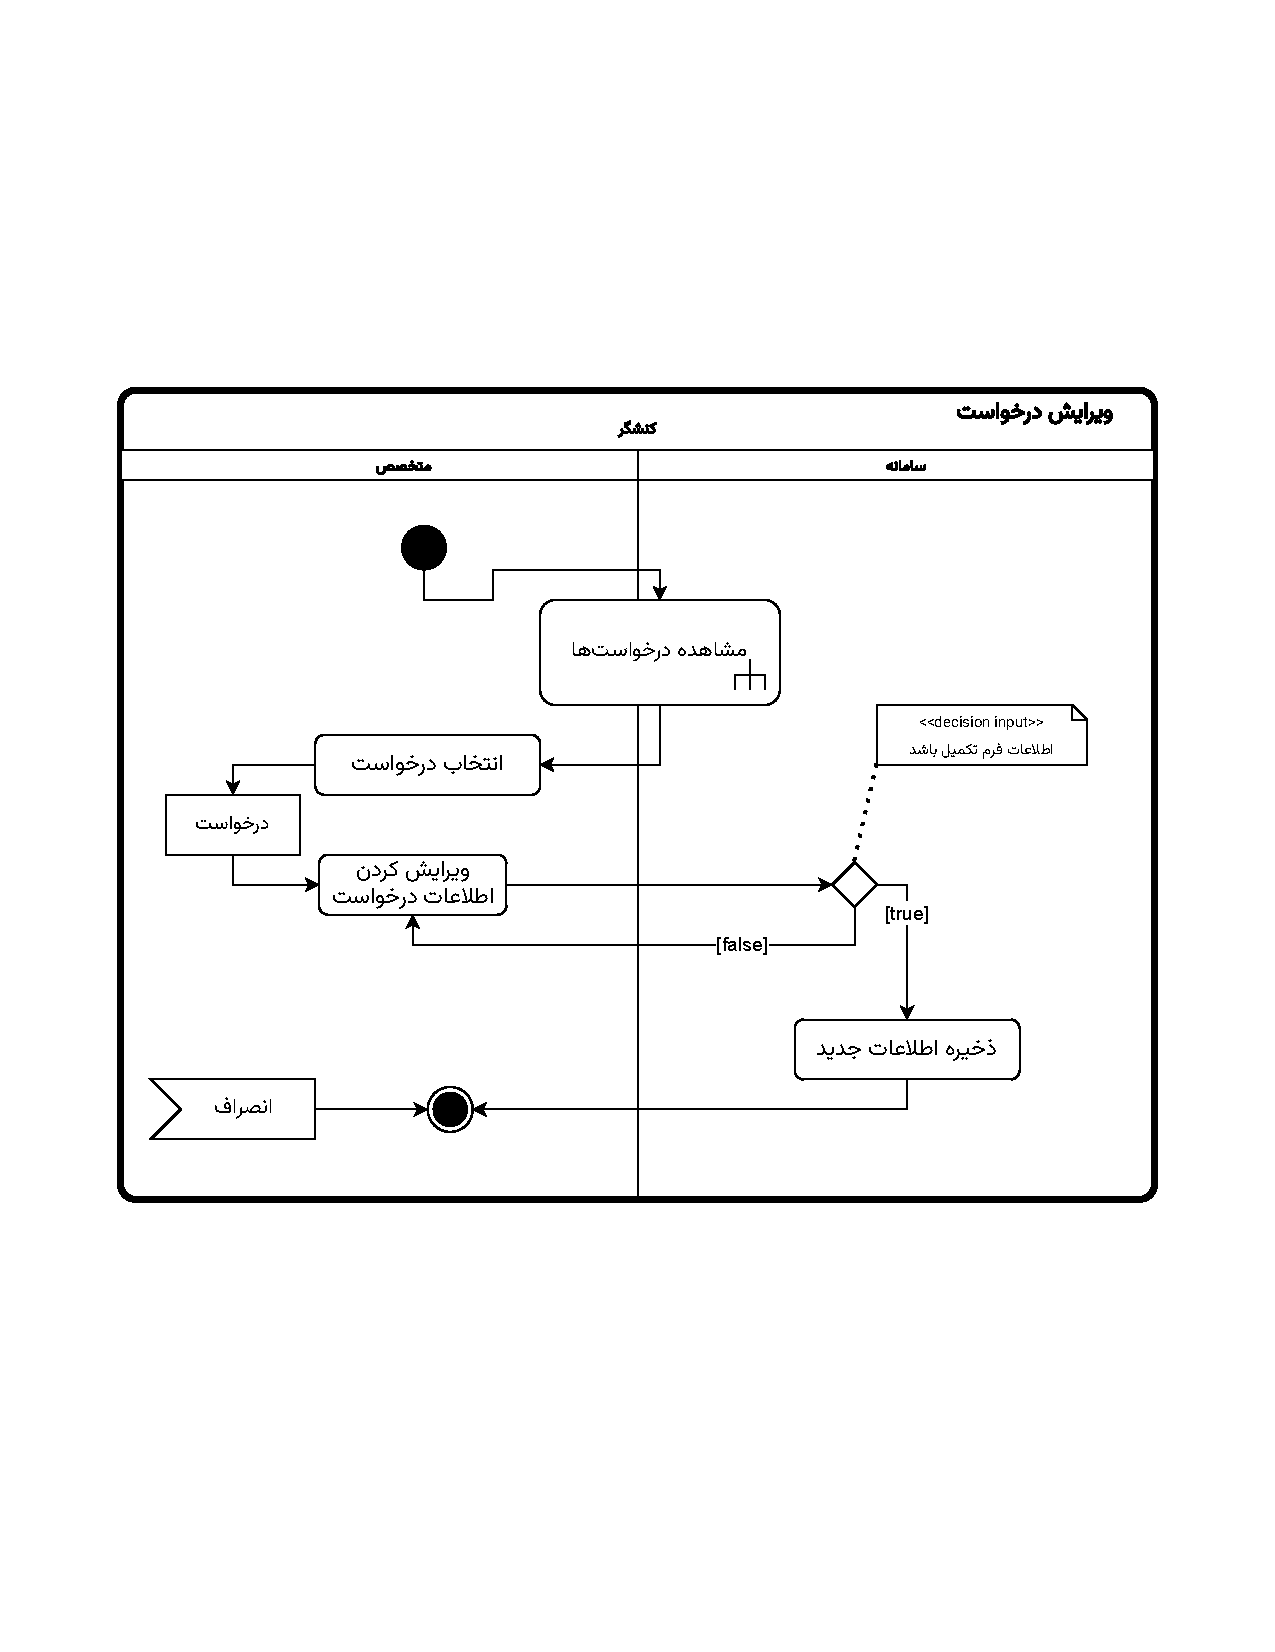
\includegraphics[scale=0.8, page=1]{figs/OOD-activity-editreq.pdf}
	\caption{نمودار فعالیت: ویرایش درخواست}
\end{figure}
\FloatBarrier
\newpage


\section{زیرسیستم بازخورد}


\begin{figure}[ht!]
	\centering
	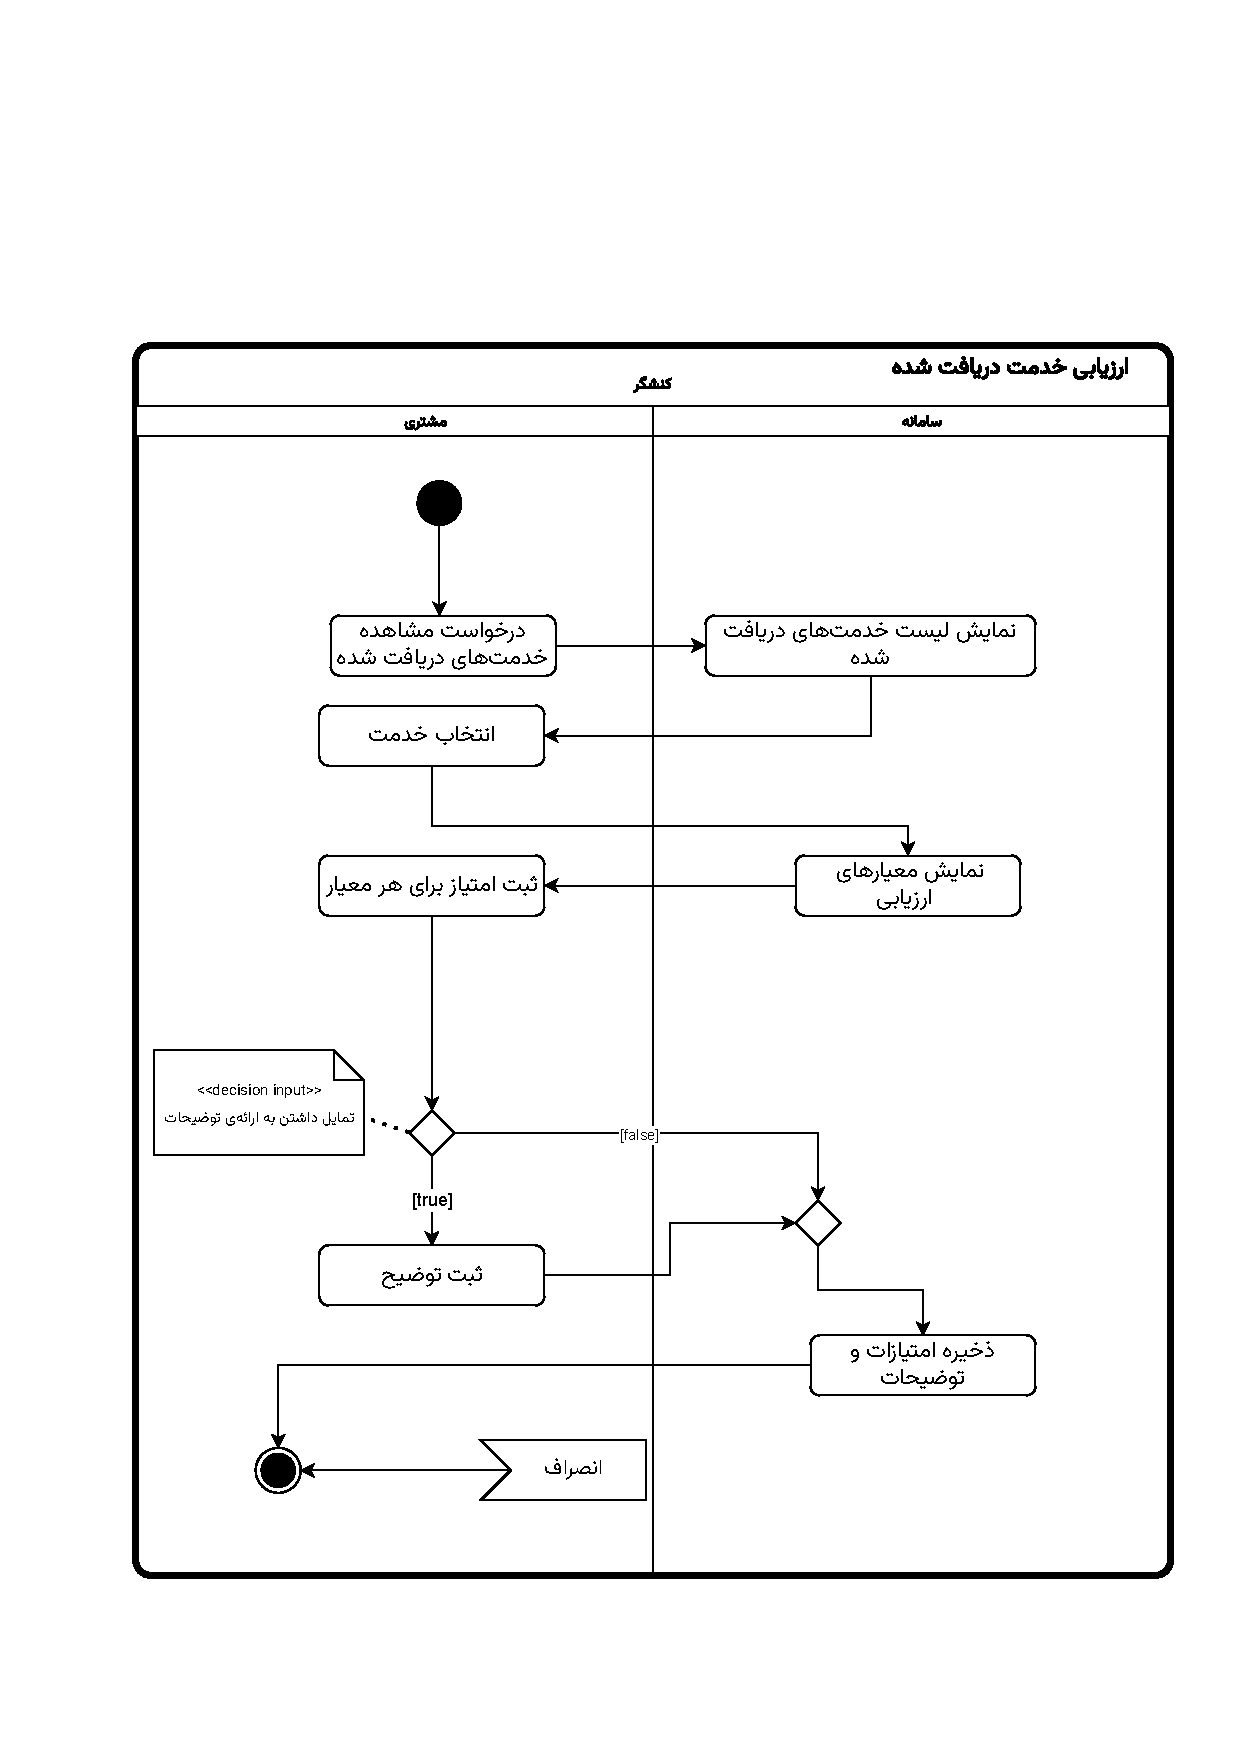
\includegraphics[scale=0.6, page=1]{figs/OOD-activity-evaluatereqrecv.pdf}
	\caption{نمودار فعالیت: ارزیابی خدمت دریافت شده}
\end{figure}
\FloatBarrier
\newpage

\begin{figure}[ht!]
	\centering
	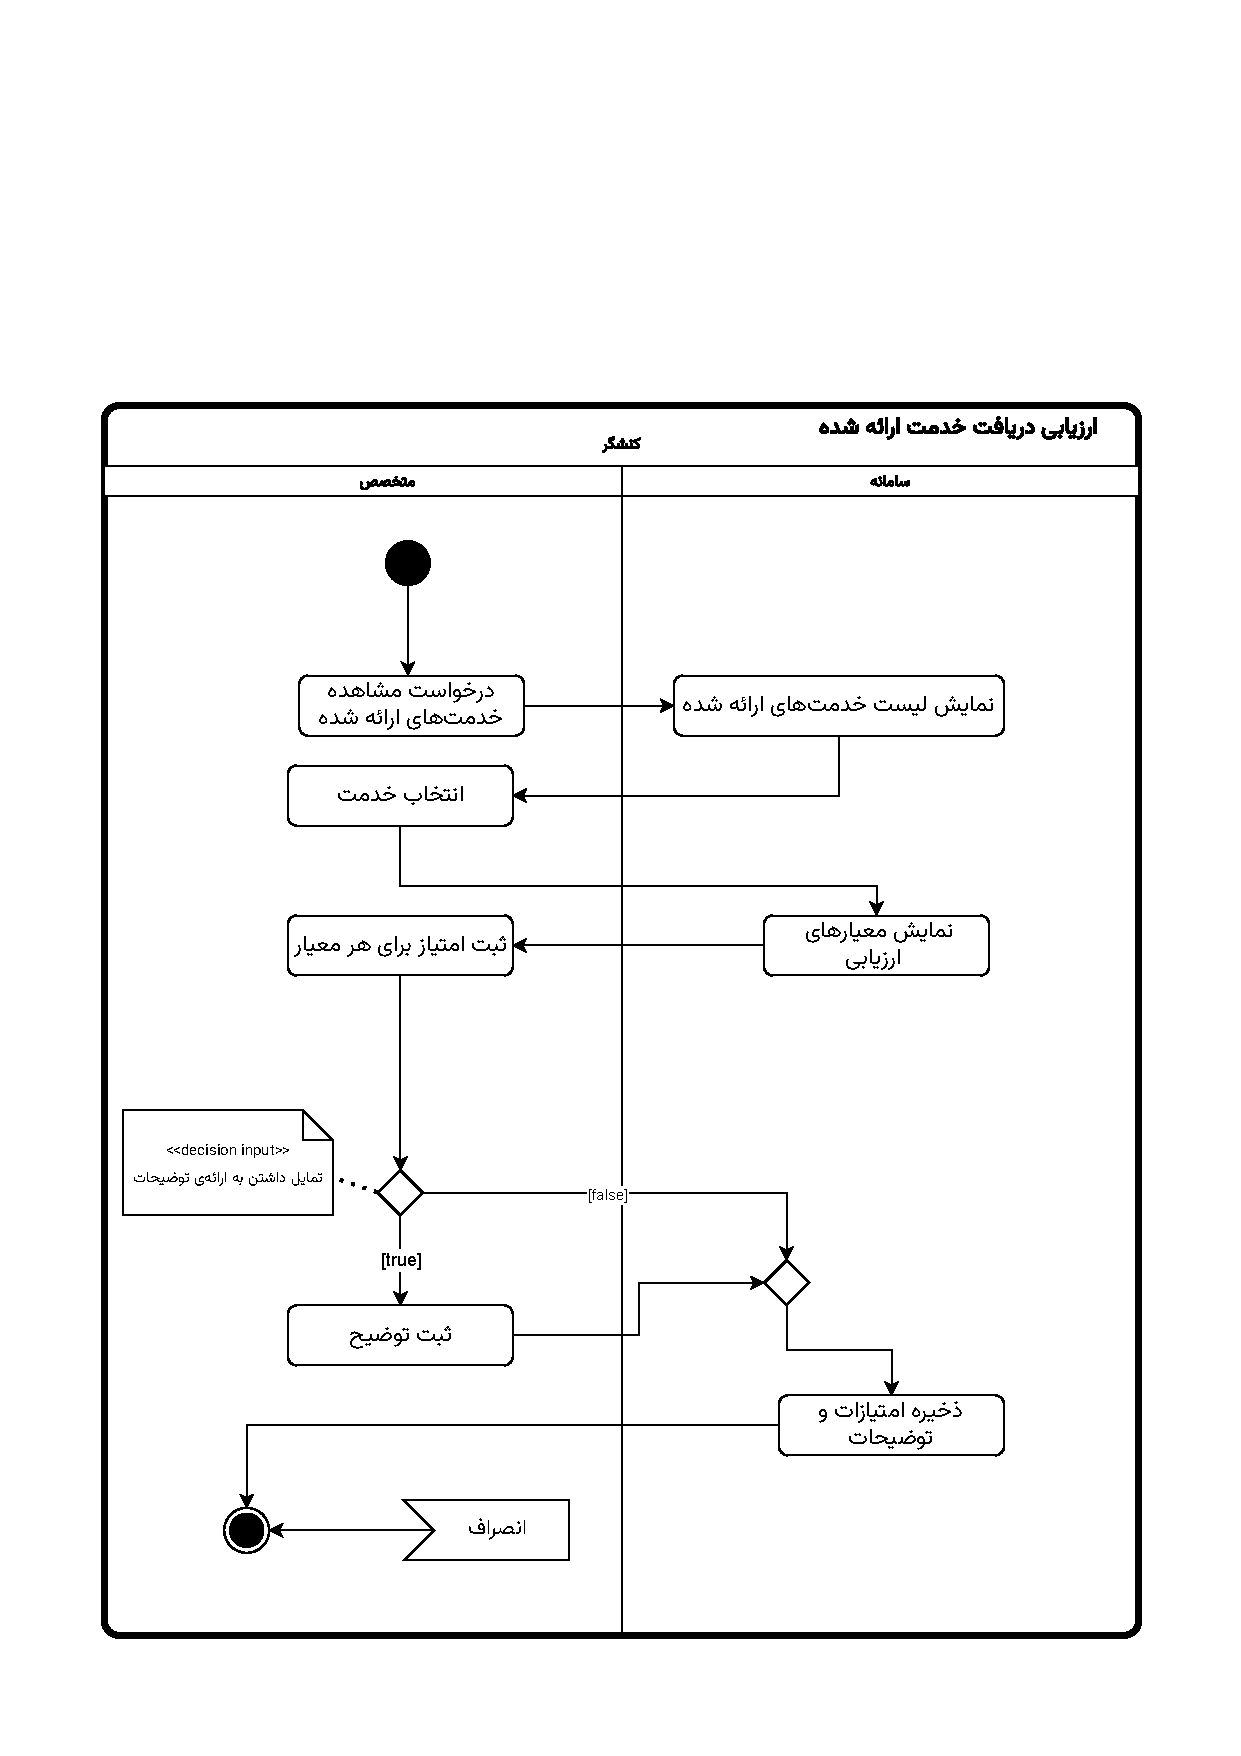
\includegraphics[scale=0.8, page=1]{figs/OOD-activity-evaluatereqsent.pdf}
	\caption{نمودار فعالیت: ارزیابی دریافت خدمت ارائه شده}
\end{figure}
\FloatBarrier
\newpage

\begin{figure}[ht!]
	\centering
	\includegraphics[scale=0.8, page=1]{figs/OOD-activity-viewevalmetric.pdf}
	\caption{نمودار فعالیت: مشاهده لیست معیارهای ارزیابی}
\end{figure}
\FloatBarrier
\newpage

\begin{figure}[ht!]
	\centering
	\includegraphics[scale=0.8, page=1]{figs/OOD-activity-addeval.pdf}
	\caption{نمودار فعالیت: اضافه کردن معیار ارزیابی}
\end{figure}
\FloatBarrier
\newpage

\begin{figure}[ht!]
	\centering
	\includegraphics[scale=0.8, page=1]{figs/OOD-activity-editeval.pdf}
	\caption{نمودار فعالیت: ویرایش معیار ارزیابی}
\end{figure}
\FloatBarrier
\newpage

\begin{figure}[ht!]
	\centering
	\includegraphics[scale=0.8, page=1]{figs/OOD-activity-deleteeval.pdf}
	\caption{نمودار فعالیت: حذف معیار ارزیابی}
\end{figure}
\FloatBarrier
\newpage

\begin{figure}[ht!]
	\centering
	\includegraphics[scale=0.8, page=1]{figs/OOD-activity-contactus.pdf}
	\caption{نمودار فعالیت: ارسال پیشنهادات و انتقادات}
\end{figure}
\FloatBarrier
\newpage


\section{زیرسیستم گزارش‌گیری}


\begin{figure}[ht!]
	\centering
	\includegraphics[scale=0.6, page=1]{figs/OOD-activity-syslog.pdf}
	\caption{نمودار فعالیت: مشاهده لاگ‌های سیستم}
\end{figure}
\FloatBarrier
\newpage

\begin{figure}[ht!]
	\centering
	\includegraphics[scale=0.8, page=1]{figs/OOD-activity-vaziatreq.pdf}
	\caption{نمودار فعالیت: دریافت وضعیت درخواست های خدمت}
\end{figure}
\FloatBarrier
\newpage

\begin{figure}[ht!]
	\centering
	\includegraphics[scale=0.8, page=1]{figs/OOD-activity-filterreqrep.pdf}
	\caption{نمودار فعالیت: فیلتر کردن درخواست های خدمت}
\end{figure}
\FloatBarrier
\newpage


\begin{figure}[ht!]
	\centering
	\includegraphics[scale=0.8, page=1]{figs/OOD-activity-reqnot.pdf}
	\caption{نمودار فعالیت: دریافت خدمات مورد تقاضا ارائه نشده}
\end{figure}
\FloatBarrier
\newpage


\begin{figure}[ht!]
	\centering
	\includegraphics[scale=0.8, page=1]{figs/OOD-activity-popular.pdf}
	\caption{نمودار فعالیت: دریافت لیست خدمات پرتقاضا و کم تقاضا}
\end{figure}
\FloatBarrier
\newpage


\begin{figure}[ht!]
	\centering
	\includegraphics[scale=0.8, page=1]{figs/OOD-activity-quality.pdf}
	\caption{نمودار فعالیت: دریافت لیست خدمات با کیفیت بالا و کیفیت پایین}
\end{figure}
\FloatBarrier
\newpage

\begin{figure}[ht!]
	\centering
	\includegraphics[scale=0.8, page=1]{figs/OOD-activity-angry.pdf}
	\caption{نمودار فعالیت: دریافت گزارش کاربران ناراضی از خدمات}
\end{figure}
\FloatBarrier
\newpage


\begin{figure}[ht!]
	\centering
	\includegraphics[scale=0.8, page=1]{figs/OOD-activity-techrep.pdf}
	\caption{نمودار فعالیت: دریافت گزارشات مشکلات فنی}
\end{figure}
\FloatBarrier
\newpage

\begin{figure}[ht!]
	\centering
	\includegraphics[scale=0.8, page=1]{figs/OOD-activity-techrepans.pdf}
	\caption{نمودار فعالیت: پاسخ گزارشات مشکل فنی}
\end{figure}
\FloatBarrier
\newpage



\section{زیرسیستم مدیریت}


\begin{figure}[ht!]
	\centering
	\includegraphics[scale=0.6, page=1]{figs/OOD-activity-getspec.pdf}
	\caption{نمودار فعالیت: دریافت تخصص‌ها}
\end{figure}
\FloatBarrier
\newpage


\begin{figure}[ht!]
	\centering
	\includegraphics[scale=0.8, page=1]{figs/OOD-activity-nokhedmatjadid.pdf}
	\caption{نمودار فعالیت: اضافه کردن تخصص جدید}
\end{figure}
\FloatBarrier
\newpage


\begin{figure}[ht!]
	\centering
	\includegraphics[scale=0.8, page=1]{figs/OOD-activity-zirhozeh.pdf}
	\caption{نمودار فعالیت: تعریف زیرحوزه برای تخصص}
\end{figure}
\FloatBarrier
\newpage


\begin{figure}[ht!]
	\centering
	\includegraphics[scale=0.8, page=1]{figs/OOD-activity-reqscore.pdf}
	\caption{نمودار فعالیت: اضافه کردن امتیاز مورد نیاز برای پذیرش درخواست}
\end{figure}
\FloatBarrier
\newpage

\begin{figure}[ht!]
	\centering
	\includegraphics[scale=0.8, page=1]{figs/OOD-activity-editreqscore.pdf}
	\caption{نمودار فعالیت: ویرایش یا حذف امتیاز مورد نیاز برای پذیرش درخواست}
\end{figure}
\FloatBarrier
\newpage

\begin{figure}[ht!]
	\centering
	\includegraphics[scale=0.8, page=1]{figs/OOD-activity-editall.pdf}
	\caption{نمودار فعالیت: ویرایش همه‌ی اطلاعات}
\end{figure}
\FloatBarrier
\newpage



\section{زیرسیستم چت}


\begin{figure}[ht!]
	\centering
	\includegraphics[scale=0.8, page=1]{figs/OOD-activity-chat.pdf}
	\caption{نمودار فعالیت: مشاهده‌ی پیام‌ها}
\end{figure}
\FloatBarrier
\newpage

\begin{figure}[ht!]
	\centering
	\includegraphics[scale=0.8, page=2]{figs/OOD-activity-chat.pdf}
	\caption{نمودار فعالیت: ارسال پیام}
\end{figure}
\FloatBarrier
\newpage


	\chapter{نمودارهای توالی}

نمودارهای توالی مربوط به هریک از موارد کاربرد (با نام مشابه) به تفکیک زیرسیستم در این بخش ارائه می‌شود.

\newpage

	

\chapter{نمودار کلاس طراحی و  نمودار مولفه}
\label{chapter:classDesign}

در ادامه نمودار کلاس‌های طراحی و مولفه‌ها قرار گرفته است.

%\KOMAoptions{paper=a2}
%\recalctypearea
\eject \pdfpagewidth=13in \pdfpageheight=15in

\begin{figure}[ht!]
	\centering
	\includegraphics[scale=0.8]{figs/design-class/comps.pdf}
	\caption{مولفه‌ها}
\end{figure}
\FloatBarrier
\newpage

\eject \pdfpagewidth=18in \pdfpageheight=17in

\begin{figure}[ht!]
	\centering
	\includegraphics[scale=0.8]{figs/design-class/requests.pdf}
	\caption{کلاس‌های طراحی مولفه درخواست}
\end{figure}
\FloatBarrier
\newpage


\eject \pdfpagewidth=15in \pdfpageheight=20in

\begin{figure}[ht!]
	\centering
	\includegraphics[scale=0.8]{figs/design-class/users.pdf}
	\caption{کلاس‌های طراحی مولفه کاربران}
\end{figure}
\FloatBarrier
\newpage


\eject \pdfpagewidth=18in \pdfpageheight=18in

\begin{figure}[ht!]
	\centering
	\includegraphics[scale=0.8]{figs/design-class/feedback.pdf}
	\caption{کلاس‌های طراحی مولفه بازخورد}
\end{figure}
\FloatBarrier
\newpage

\eject  \pdfpagewidth=10in \pdfpageheight=10in

\begin{figure}[ht!]
	\centering
	\includegraphics[scale=0.8]{figs/design-class/reports.pdf}
	\caption{کلاس‌های طراحی مولفه گزارش‌گیری}
\end{figure}
\FloatBarrier
\newpage

\KOMAoptions{paper=a4}
\recalctypearea

\begin{figure}[ht!]
	\centering
	\includegraphics[scale=0.8]{figs/design-class/chat.pdf}
	\caption{کلاس‌های طراحی مولفه چت}
\end{figure}
\FloatBarrier
\newpage

\begin{figure}[ht!]
	\centering
	\includegraphics[scale=0.8]{figs/design-class/utils.pdf}
	\caption{کلاس‌های طراحی \lr{utility}}
\end{figure}
\FloatBarrier
\newpage

\eject \pdfpagewidth=16in \pdfpageheight=12in
\begin{figure}[ht!]
	\centering
	\includegraphics[scale=0.8]{figs/design-class/rest.pdf}
	\caption{کلاس‌های طراحی مولفه فریم‌ورک رست}
\end{figure}
\FloatBarrier
\newpage

\KOMAoptions{paper=a4}
\recalctypearea

\begin{figure}[ht!]
	\centering
	\includegraphics[scale=0.8]{figs/design-class/db.pdf}
	\caption{کلاس‌های طراحی مولفه دیتابیس}
\end{figure}
\FloatBarrier
\newpage

\eject \pdfpagewidth=25in \pdfpageheight=25in

\begin{figure}[ht!]
	\centering
	\includegraphics[scale=0.8]{figs/design-class/front.pdf}
	\caption{کلاس‌های طراحی رابط کاربری}
\end{figure}
\FloatBarrier
\newpage

\KOMAoptions{paper=a4}
\recalctypearea

هر کدام از این کلاس‌های سریالایزر که در ادامه آورده شده در مولفه‌های مربوط به خودشان قرار می‌گیرند و برای سریالایز کردن آبجکت‌های مختلف و تبدیل آن‌ها به JSON استفاده می‌شوند. برای پرهیز از شلوغی مولفه‌ها به طور جداگانه آورده‌شده‌اند.

هم چنین همه‌ی این کلاس‌ها از کلاس
\lr{rest\_framework.ModelSerializer}
ارث‌بری می‌کنند.

\begin{figure}[ht!]
	\centering
	\includegraphics[scale=0.8]{figs/design-class/serial.pdf}
	\caption{کلاس‌های سریالایزر}
\end{figure}
\FloatBarrier
\newpage


\KOMAoptions{paper=a4}
\recalctypearea
\newpage

% figs/OOD-design-class-page-1.pdf
	\chapter{نمودارهای توالی طراحی}


نمودارهای توالی طراحی مربوط به هریک از موارد کاربرد (با نام مشابه) به تفکیک زیرسیستم در این بخش ارائه می‌شود.



\begin{figure}[ht!]
	\centering
	\includegraphics[scale=0.8]{figs/design-sequence/reusable.pdf}
	\caption{قطعه نمودارهای توالی قابل استفاده مجدد}
\end{figure}
\FloatBarrier
\newpage


\section{زیرسیستم کاربری}

\eject \pdfpagewidth=12in \pdfpageheight=7in
\begin{figure}[ht!]
	\centering
	\includegraphics[scale=0.8]{figs/design-sequence/3-1.pdf}
	\caption{نمودار توالی طراحی: ثبت نام}
\end{figure}
\FloatBarrier
\newpage

\eject \pdfpagewidth=11in \pdfpageheight=7in
\begin{figure}[ht!]
	\centering
	\includegraphics[scale=0.8]{figs/design-sequence/3-2.pdf}
	\caption{نمودار توالی طراحی: ورود}
\end{figure}
\FloatBarrier
\newpage

\section{زیرسیستم خدمت‌دهی}

\eject \pdfpagewidth=11in \pdfpageheight=7in

\begin{figure}[ht!]
	\centering
	\includegraphics[scale=0.8]{figs/design-sequence/3-10.pdf}
	\caption{نمودار توالی طراحی: مشاهده درخواست‌ها}
\end{figure}
\FloatBarrier
\newpage

\eject \pdfpagewidth=10in \pdfpageheight=10in

\begin{figure}[ht!]
	\centering
	\includegraphics[scale=0.8]{figs/design-sequence/3-11.pdf}
	\caption{نمودار توالی طراحی: مشاهده جزئیات درخواست}
\end{figure}
\FloatBarrier
\newpage

\eject \pdfpagewidth=15in \pdfpageheight=12in

\begin{figure}[ht!]
	\centering
	\includegraphics[scale=0.8]{figs/design-sequence/3-16.pdf}
	\caption{نمودار توالی طراحی: لغو درخواست خدمت}
\end{figure}
\FloatBarrier
\newpage


\eject \pdfpagewidth=12in \pdfpageheight=8in

\begin{figure}[ht!]
	\centering
	\includegraphics[scale=0.8]{figs/design-sequence/3-17.pdf}
	\caption{نمودار توالی طراحی: جست‌وجو و مشاهده متخصصین}
\end{figure}
\FloatBarrier
\newpage

\eject \pdfpagewidth=15in \pdfpageheight=12in

\begin{figure}[ht!]
	\centering
	\includegraphics[scale=0.8]{figs/design-sequence/3-18.pdf}
	\caption{نمودار توالی طراحی: ثبت درخواست}
\end{figure}
\FloatBarrier
\newpage



\section{زیرسیستم بازخورد}

\eject \pdfpagewidth=17in \pdfpageheight=8in

\begin{figure}[ht!]
	\centering
	\includegraphics[scale=0.8]{figs/design-sequence/3-24.pdf}
	\caption{نمودار توالی طراحی: ارزیابی خدمت دریافت شده}
\end{figure}
\FloatBarrier
\newpage

\eject \pdfpagewidth=17in \pdfpageheight=8in


\begin{figure}[ht!]
	\centering
	\includegraphics[scale=0.8]{figs/design-sequence/3-25.pdf}
	\caption{نمودار توالی طراحی: ارزیابی دریافت خدمت ارائه شده}
\end{figure}
\FloatBarrier
\newpage

\eject \pdfpagewidth=13in \pdfpageheight=6in


\begin{figure}[ht!]
	\centering
	\includegraphics[scale=0.8]{figs/design-sequence/3-26.pdf}
	\caption{نمودار توالی طراحی: مشاهده لیست معیارهای ارزیابی}
\end{figure}
\FloatBarrier
\newpage

\eject \pdfpagewidth=10in \pdfpageheight=8in

\begin{figure}[ht!]
	\centering
	\includegraphics[scale=0.8]{figs/design-sequence/3-27.pdf}
	\caption{نمودار توالی طراحی: اضافه کردن معیار ارزیابی}
\end{figure}
\FloatBarrier
\newpage

\eject \pdfpagewidth=12in \pdfpageheight=11in

\begin{figure}[ht!]
	\centering
	\includegraphics[scale=0.8]{figs/design-sequence/3-28.pdf}
	\caption{نمودار توالی طراحی: ویرایش معیار ارزیابی}
\end{figure}
\FloatBarrier
\newpage

\eject \pdfpagewidth=12in \pdfpageheight=11in
\begin{figure}[ht!]
	\centering
	\includegraphics[scale=0.8]{figs/design-sequence/3-29.pdf}
	\caption{نمودار توالی طراحی: حذف معیار ارزیابی}
\end{figure}
\FloatBarrier
\newpage

\eject \pdfpagewidth=10in \pdfpageheight=9in

\begin{figure}[ht!]
	\centering
	\includegraphics[scale=0.8]{figs/design-sequence/3-30.pdf}
	\caption{نمودار توالی طراحی: ارسال پیشنهادات و انتقادات}
\end{figure}

\FloatBarrier
\newpage

\section{زیرسیستم مدیریت}

\eject \pdfpagewidth=13in \pdfpageheight=9in

\FloatBarrier
\begin{figure}[ht!]
	\centering
	\includegraphics[scale=0.8]{figs/design-sequence/3-39.pdf}
	\caption{نمودار توالی طراحی: دریافت گزارش مشکلات فنی}
\end{figure}
\FloatBarrier
\newpage

\eject \pdfpagewidth=11in \pdfpageheight=9in


\begin{figure}[ht!]
	\centering
	\includegraphics[scale=0.8]{figs/design-sequence/3-40.pdf}
	\caption{نمودار توالی طراحی: پاسخ به گزارش مشکلات فنی}
\end{figure}

\FloatBarrier
\newpage

\eject \pdfpagewidth=10in \pdfpageheight=9in

\section{زیرسیستم چت}

\begin{figure}[ht!]
	\centering
	\includegraphics[scale=0.8]{figs/design-sequence/3-47.pdf}
	\caption{نمودار توالی طراحی: مشاهده‌ی پیام‌ها}
\end{figure}
\FloatBarrier
\newpage

\eject \pdfpagewidth=10in \pdfpageheight=9in
\begin{figure}[ht!]
	\centering
	\includegraphics[scale=0.8]{figs/design-sequence/3-48.pdf}
	\caption{نمودار توالی طراحی: ارسال پیام}
\end{figure}
\FloatBarrier
\newpage





\KOMAoptions{paper=a4}
\recalctypearea
\newpage

	\chapter{
شمای پایگاه داده
}

در این فصل شمای
\footnote{\lr{schema}}
 پایگاه داده مشخص شده است. در هر جدول نوع مقدار، کلیدهای اصلی، کلیدهای خارجی، قابل تهی
\footnote{\lr{Null}}
 بودن مقدار و همچنین متمایز
 \footnote{\lr{Unique}}
  بودن آن مشخص شده است.
\begin{figure}[h]
	\centering
	\includegraphics[width=\textwidth]{figs/entity-relationship}
	\caption{شمای پایگاه داده}
	\label{database-schema}
\end{figure}


	\chapter{
الگوهای طراحی
}

در این فصل اجمالا الگوهای طراحی اصلی استفاده شده در پروژه ذکر شده است. الگوهای استفاده شده در بک‌اند در قسمت \ref{designpattern:back} و الگوهای استفاده شده در فرانت‌اند در قسمت \ref{designpattern:front} آورده شده‌اند.

\newpage
\section{بک‌اند}
\label{designpattern:back}

\begin{itemize}
	\item 
	\textbf{الگوی \lr{Singleton}}
	از این الگو برای کلاس‌هایی که می‌خواهیم تنها یک Instance از آن‌ها موجود باشد استفاده کرده‌ایم. استفاده اصلی آن برای کلاس‌های کاتالوگ (نظیر \lr{UserCatalogue}، \lr{RequestCatalogue} و...) بوده است که وظیفه جست‌وجو روی کلاس‌های نظیر خود را دارند. نحوه پیاده‌سازی این مورد به صورت تعریف یک کلاس \lr{Singleton} بوده است که بقیه کلاس‌ها با عملیاتی مشابه ارث‌بری از آن استفاده می‌کنند. البته به خاطر ساختار خاص پایتون، در اصل این فرآیند ارث‌بری مستقیم نیست و از طریق \lr{metaclass} مهیا شده است که تفاوت‌های اندکی در لایه درونی پیاده‌سازی پایتون با ارث‌بری دارد ولی در نمودارها به صورت ارث‌بری نشان داده شده است چون از نظر عملکردی مشابه ارث‌بری عمل می‌کند.
	
	\item 
	\textbf{الگوی \lr{Iterator}}
	این الگو عملا در سطح خود پایتون پیاده سازی شده است و به ما اجازه استفاده از \lr{for} روی \lr{Collection} های مختلف نظیر \lr{List} ها بدون نیاز به دسترسی مستقیم به اندیس‌های آن را می‌دهد. از آن جایی که در بسیاری از قسمت‌های مختلف که بر روی لیستی از رشته‌ها یا آی‌دی‌ها و آبجکت‌ها عملیاتی انجام شده است، از این الگو استفاده شده، در این قسمت آن را ذکر کرده ایم.
	
	\item 
	\textbf{الگوی \lr{Abstract Factory}}ی
	
	یکی از مواردی که در کد به آن نیاز داشتیم، \lr{Permission} های مختلف برای \lr{Endpoint} های گوناگون بود. نحوه هندل شدن این موضوع در جنگو به این صورت است که باید کلاسی که \lr{Permission} در آن تعریف شده است به عنوان پارامتری در یک لیست به کلاسی که ریکوئست را دریافت می‌کند داده بشود. از آن‌جایی که هر بار تعریف این کلاس‌ها و آن هم برای نقش‌های گوناگون باعث ایجاد \lr{Duplicate Code} بسیار زیادی می‌شد، ما از الگوی \lr{Abstract Factory} استفاده کردیم. در این الگو یک کلاس \lr{PermissionFactory} داریم که با دریافت نوع کاربری که باید برای آن \lr{Permission} تعریف بشود، کلاس پایتونی مد نظر برای آن را ایجاد کرده و به ما تحویل می‌دهد تا در قسمت‌های مختلف کد استفاده کنیم. بدین ترتیب فقط یک بار نحوه ایجاد این کلاس در \lr{PermissionFactory} نوشته شده و این \lr{PermissionFactory} است که وظیفه ایجاد این کلاس را بر عهده دارد.
	
	\item
	\textbf{الگوی \lr{Builder}}
	
	از این الگو برای ایجاد \lr{Notification} ها استفاده شده است. از آن جایی که متن درون هر \lr{Notification} به نوع آن \lr{Notification} و محل استفاده آن بستگی دارد ولی الگوی کلی ساخته شدن آن (یعنی تعریف عنوان، تعریف بدنه، تعریف کاربر و...) یکسان است، از الگوی \lr{Builder} استفاده شده است. در کلاس \lr{NotificationBuilder} مراحل مقداردهی پارامترهای مختلف \lr{Notification} انجام می‌شود و کلاس‌های مختلف \lr{Notification} بسته به نوع کاربردی که دارند، جزییات متن پیام و پارامترها را استخراج کرده و آن‌‌ها را در اختیار \lr{NotificationBuilder} قرار می‌دهند تا به ترتیبی که لازم است، آن‌ها را در کنار هم قرار داده و \lr{Notification} را ایجاد کند.
	
	
	\item
	\textbf{الگوی \lr{Adapter}}
	
	در بسیاری از قسمت‌هایی که سرچ انجام می‌شد، برای حالتی که \lr{ID} داده بشود، برای این که جامع‌ترین حالت پوشش داده بشود، از \lr{Syntax} ای که مخصوص جست‌وجو روی لیست است استفاده می‌شود که بتوانیم لیستی از \lr{ID} ها را داده و همه آن‌ها را تحویل بگیریم. نکته‌ای که وجود دارد این است که اگر از سمت فرانت‌اند درخواستی که برای بک‌اند می‌آید لیست نبوده و مثلا یک \lr{ID} تنها باشد، در \lr{Syntax} جنگو با مشکل مواجه می‌شویم چون انتظار لیست را داشته است. از آن‌جایی که این موضوع به کرات رخ می‌داد، برای این موضوع کلاسی به نام \lr{ListAdapter} تعریف کردیم . این کلاس تابعی به نام \verb+python_ensure_list+  داشته که یک ورودی گرفته و اگر \lr{list} باشد خود آن را بر می‌گرداند و اگر \lr{string} یا \lr{int} باشد، آن‌ را درون یک لیست تکی قرار داده و این \lr{list} را خروجی می‌دهد. بدین ترتیب نیازی به چک کردن‌های زیاد در قسمت‌هایی که انتظار ورودی دادن یک لیست را داریم نداشته و صرفا ورودی را به این \lr{Adapter} می‌دهیم تا در صورتی که در قالب مشخص ما نبود، آن را به قالبی که قابل استفاده باشد تبدیل کند.
	
	
	
\end{itemize}

\newpage

\section{فرانت‌اند}
\label{designpattern:front}


\begin{itemize}
	\item 
	\textbf{الگوی \lr{Composite}}
	در اصل استفاده از این الگو به دلیل استفاده از \lr{React} در کد ما ایجاد شده است. کامپوننت‌های \lr{React} هر کدام تابع \verb+render+ دارند که درون خود می‌تواند ساختار کامپوننت‌های دیگر را جای بدهد. نحوه کار این تابع بدین صورت است که ساختار کلی تعریف شده درون آن را ایجاد کرده و بعد \verb+render+ فرزندان درون خود را صدا می‌زند که آن‌ها هم ممکن است کامپوننت‌های \lr{React} بوده و درون خود \verb+render+ را صدا بزنند. برگ‌ها در این ساختار همان المان‌های ساده \lr{HTML} هستند که دیگر اجزای درونی‌تری نداشته و رندر می‌شوند.
	
	\item 
	\textbf{الگوی \lr{Observer}}
	در فرانت‌اند ما برای مدیریت \lr{State} از کتابخانه \lr{Redux} استفاده کرده‌ایم که عملا پیاده‌سازی‌ الگوی \lr{Observer} است. در \lr{Redux}، حالات مورد نیاز هر کدام از کامپوننت‌ها در مجموعه‌ای که به طور کلی \lr{Store} نامیده می‌شود قرار می‌گیرند و هر کدام از کامپوننت‌ها بسته به این که به کدام بخش از داده‌های درون \lr{Store} نیاز دارند، مشترک آن قسمت شده و در صورت تغییرات آن، از آن مطلع شده و تغییرات لازم در آن‌ها اعمال می‌شود.
	
	 
\end{itemize}
	\chapter{ارزیابی دستاوردهای تکرار}
در این بخش محصولات تکرار با استفاده از تعدادی معیار سنجیده می‌شوند. این معیارها با توجه به محصولات هر تکرار، به‌روزرسانی و تکمیل خواهند شد.
\section{چک‌لیست‌های ارزیابی}

\iffalse
Item icons for checklists:	
	\item[$\square$]
	\item[$\boxtimes$]
\fi

\subsection{اهداف کلی فاز}
در این قسمت دستاوردهایی که باید در فاز تفصیل تحقق یابد، بررسی می‌شود. از آنجا که این اهداف باید در طول سه تکرار محقق شوند، این لیست به‌مرور تکمیل خواهد شد:
\begin{itemize} % \setlength\itemsep{0.1cm}
	\item[$\boxtimes$]
	ایجاد نرم‌افزار اجرایی پایه‌ی معماری\LTRfootnote{Executable architectural baseline}
	\item[$\square$]
	تکمیل نرم‌افزار اجرایی
	\item[$\boxtimes$]
	تعریف حدود 80 درصد از نیازمندی‌های وظیفه‌ای سیستم
	\item[$\square$]
	تعریف شاخصه‌های کیفیت (مانند نرخ یافتن نقص)
	\item[$\square$]
	ایجاد یک برنامه با جزئیات برای فاز construction
	
\end{itemize}

\subsection{کارت‌های \lr{CRC}}

\begin{itemize}
	\item[$\boxtimes$]
	تفکیک مسئولیت‌های مختلف هر کلاس در سطرهای جداگانه
	\item[$\boxtimes$]
	نام کلاس نشان‌گر منظور آن باشد و به یک وجهه از قلمرو مسئله نگاشت شود.
	\item[$\boxtimes$]
	لیست مسئولیت‌ها کوتاه و خوش‌تعریف باشد.
	\item[$\boxtimes$]
	ویژگی‌های کلاس انسجام\LTRfootnote{\lr{Cohesion}} بالایی داشته باشند.
	\item[$\boxtimes$]
	میزان جفت‌شدگی\LTRfootnote{\lr{Coupling}} با سایر کلاس‌ها پایین باشد (برای تحقق منظور خود نیاز به ارتباط با تعداد کمی کلاس دیگر داشته باشد).
	\item[$\boxtimes$]
	کلاس‌های بسیار کوچک زیاد یا صرفاً چند کلاس بزرگ وجود نداشته باشد.
	\item[$\boxtimes$]
	هیچ کلاسی قادر مطلق نباشد و درخت وراثت عمیقی نیز نداشته باشد.

\end{itemize}

\subsection{نمودارهای فعالیت و موارد کاربرد}

\begin{itemize}
	\item[$\boxtimes$]
	ساده و کوتاه نگه داشتن نمودارهای موارد کاربرد
	\item[$\boxtimes$]
	تمرکز روی نیاز کنش‌گر از سیستم به‌جای چگونگی انجام در نمودار موارد کاربرد
	\item[$\boxtimes$]
	خودداری از \lr{Functional Decomposition} در نمودار موارد کاربرد
	\item[$\boxtimes$]
	کاربرد صحیح \lr{Notation} نمودار فعالیت (نمادها، سیگنال و رویداد و ...)
	\item[$\square$]
	استفاده صحیح از \lr{Swim Lane} در نمودار فعالیت
	
\end{itemize}

\subsection{نرم‌افزار اجرایی پایه معماری}
با توجه به زمان‌بندی و تکمیل این بخش در تکرار دوم فاز تفصیل، برخی از معیارها در تکرار بعد اضافه و تکمیل می‌شوند.
\begin{itemize}
	\item[$\square$]
	عملیات عمومی کلاس‌ها با کارخواهان یک قرارداد تعریف کند.
	\item[$\boxtimes$]
	تمامیت\LTRfootnote{\lr{Completeness}} (کاربرد کلاس کم‌تر از انتظار معقول کارخواه نباشد)
	\item[$\boxtimes$]
	کفایت\LTRfootnote{\lr{Sufficiency}} (کاربرد کلاس بیشتر از انتظار معقول کارخواه نباشد)
	\item[$\boxtimes$]
	بدوی بودن\LTRfootnote{\lr{Primitveness}} (خدمات کلاس ساده، اتمیک و منحصربه‌فرد باشد)
	\item[$\boxtimes$]
	انسجام بالا به معنی مستقل و واحد بودن مفهوم هر کلاس و پشتیبانی اعمال کلاس از منظور آن
	\item[$\boxtimes$]
	جفت‌شدگی پایین به معنی خودداری از اتصال دو کلاس بدون ازتباط معنایی صحیح و یا به جهت استفاده مجدد از کد و همچنین به معنی محدود بودن اتصالات کلاس با سایرین در حدی که منظور آن کلاس را تحقق بخشد.
\end{itemize}

	
\chapter{برنامه زمانی فازها}



با توجه به این که قرار است تمامی اعضای گروه در انجام تمامی قسمت‌ها مشارکت داشته باشند، نام افراد ذکر نشده است.




\section{تحلیل مقدماتی - تکرار اول}

\begin{table}[h]
	\centering
	\begin{tabular}{|p{0.07\linewidth}|p{0.35\linewidth}|p{0.1\linewidth}|p{0.15\linewidth}|p{0.15\linewidth}|p{0.07\linewidth}|} 
		
		\hline
		شناسه & نام وظیفه & مدت (روز) & شروع & پایان & پیش‌نیاز\\
		\hline
		\calendarEntry
		{1}
		{تخمین زمانی برای پروژه}
		{1}
		{2/30}
		{2/30}
		{}
		\calendarEntry
		{2}
		{تهیه قالب مستندات}
		{0.5}
		{2/31}
		{2/31}
		{}
		
		\calendarEntry
		{3}
		{تهیه لیست ریسک‌ها}
		{0.5}
		{2/31}
		{2/31}
		{1}
		
			\calendarEntry
		{4}
		{تهیه لیست نیازمندی‌ها}
		{0.5}
		{3/1}
		{3/1}
		{1}
		
			\calendarEntry
		{5}
		{اولویت بندی نیازمندی‌ها و ریسک‌ها}
		{0.5}
		{3/1}
		{3/1}
		{3,4}
		
		
			\calendarEntry
		{6}
		{رسم نمودار موارد کاربرد}
		{0.5}
		{3/2}
		{3/2}
		{5}
		
					\calendarEntry
		{7}
		{جزییات موارد کاربرد}
		{2}
		{3/2}
		{3/4}
		{6}
		
					\calendarEntry
		{8}
		{تکمیل واژه‌نامه و موارد باقی‌مانده مستندات}
		{0.5}
		{3/4}
		{3/4}
		{7}
		
		
	\end{tabular}
\end{table}



\section{تحلیل تفصیلی - تکرار اول}

\begin{table}[h]
	\centering
	\begin{tabular}{|p{0.07\linewidth}|p{0.35\linewidth}|p{0.1\linewidth}|p{0.15\linewidth}|p{0.15\linewidth}|p{0.07\linewidth}|} 
		
		\hline
		شناسه & نام وظیفه & مدت (روز) & شروع & پایان & پیش‌نیاز\\
		\hline
		\calendarEntry
		{9}
		{بروزرسانی ریسک‌ها، نیازمندی‌ها و زمان‌بندی}
		{1}
		{3/5}
		{3/5}
		{3,4,1}
		
				\calendarEntry
		{10}
		{تهیه \lr{Architecturally Significant Requirements}}
		{1}
		{3/6}
		{3/6}
		{9}
		
		
						\calendarEntry
		{11}
		{\lr{Use Case Realization}}
		{2}
		{3/7}
		{3/9}
		{10}
		
		
		
				
		\calendarEntry
		{12}
		{کارت‌های \lr{CRC}}
		{1}
		{3/9}
		{3/10}
		{11}
		
		
			\calendarEntry
		{13}
		{پیاده‌سازی \lr{Executable Architectural Baseline}}
		{4}
		{3/10}
		{3/14}
		{12}
		
		
					\calendarEntry
		{14}
		{ارزیابی دستاورد‌های تکرار}
		{0.5}
		{3/15}
		{3/15}
		{13}
		
		
				
		\calendarEntry
		{15}
		{تکمیل مستندات}
		{0.5}
		{3/15}
		{3/15}
		{14}
		
		
		
		

	\end{tabular}
\end{table}

\newpage

\section{تحلیل تفصیلی - تکرار دوم}


\begin{table}[h]
	\centering
	\begin{tabular}{|p{0.07\linewidth}|p{0.35\linewidth}|p{0.1\linewidth}|p{0.15\linewidth}|p{0.15\linewidth}|p{0.07\linewidth}|} 
		
		\hline
		شناسه & نام وظیفه & مدت (روز) & شروع & پایان & پیش‌نیاز\\
		\hline
		\calendarEntry
		{16}
		{بروزرسانی محصولات نیازمندی فاز قبل}
		{0.5}
		{3/16}
		{3/16}
		{15}
		

		\calendarEntry
{17}
{تهیه واسط کاربری قابل اجرا و تصویر از آن}
{2.5}
{3/16}
{3/18}
{16}
	
	
			\calendarEntry
	{18}
	{بروزرسانی محصولات تحلیل فاز قبل}
	{1}
	{3/18}
	{3/19}
	{16}
	
	
	
				\calendarEntry
	{19}
	{تهیه نمودار فعالیت با خطوط شنا}
	{2}
	{3/19}
	{3/21}
	{18}
	
	
					\calendarEntry
	{20}
	{نمودار کلاس تحلیل}
	{1}
	{3/21}
	{3/22}
	{19}
	
	
					\calendarEntry
	{21}
	{نمودار توالی تحلیل}
	{1}
	{3/22}
	{3/23}
	{19}
	
	
					\calendarEntry
	{22}
	{نمودار بسته}
	{1}
	{3/23}
	{3/24}
	{20,21}
	
	
					\calendarEntry
	{23}
	{ارزیابی دستاورد‌های تکرار}
	{0.5}
	{3/24}
	{3/24}
	{22}
	
	
	
	\calendarEntry
	{24}
	{تکمیل مستندات}
	{1.5}
	{3/24}
	{3/26}
	{23}
		
		
		
	\end{tabular}
\end{table}

\newpage


\section{تحلیل تفصیلی - تکرار سوم}


\begin{table}[h]
	\centering
	\begin{tabular}{|p{0.07\linewidth}|p{0.35\linewidth}|p{0.1\linewidth}|p{0.15\linewidth}|p{0.15\linewidth}|p{0.07\linewidth}|} 
		
		\hline
		شناسه & نام وظیفه & مدت (روز) & شروع & پایان & پیش‌نیاز\\
		\hline
		\calendarEntry
		{25}
		{بروزرسانی محصولات نیازمندی فاز قبل}
		{0.5}
		{3/26}
		{3/26}
		{24}
		
		
				\calendarEntry
		{26}
		{بروزرسانی محصولات تحلیل فاز قبل}
		{0.5}
		{3/26}
		{3/26}
		{24}



				\calendarEntry
{27}
{نمودار کلاس طراحی}
{4}
{3/26}
{3/30}
{26}

				\calendarEntry
{28}
{نمودار مولفه}
{2}
{4/16}
{4/18}
{27}

				\calendarEntry
{28}
{نمودار توالی طراحی}
{2}
{4/18}
{4/20}
{27}
		
		
						\calendarEntry
		{29}
		{تکمیل \lr{Executable Architectural Baseline}}
		{3}
		{4/21}
		{4/24}
		{28}
		
		
								\calendarEntry
		{30}
		{ارزیابی دستاوردهای تکرار}
		{0.5}
		{4/25}
		{4/25}
		{29}
		
				
		
		\calendarEntry
		{31}
		{تکمیل مستندات}
		{0.5}
		{4/25}
		{4/25}
		{30}
	\end{tabular}
\end{table}

\newpage
\section{ساخت - تکرار اول}


\begin{table}[h]
	\centering
	\begin{tabular}{|p{0.07\linewidth}|p{0.35\linewidth}|p{0.1\linewidth}|p{0.15\linewidth}|p{0.15\linewidth}|p{0.07\linewidth}|} 
		
		\hline
		شناسه & نام وظیفه & مدت (روز) & شروع & پایان & پیش‌نیاز\\
		\hline
		\calendarEntry
		{32}
		{بروزرسانی محصولات نیازمندی فاز قبل}
		{0.5}
		{4/26}
		{4/26}
		{31}
		
		
		\calendarEntry
		{33}
		{بروزرسانی محصولات تحلیل فاز قبل}
		{0.5}
		{4/26}
		{4/26}
		{32}
		
		
			\calendarEntry
		{34}
		{بازنگری کلاس‌های طاحی و نمودار‌های توالی}
		{1}
		{4/27}
		{4/28}
		{33}
		
		
				\calendarEntry
		{35}
		{تکامل سیستم اولیه}
		{2}
		{4/28}
		{4/30}
		{34}
		
					\calendarEntry
		{36}
		{توضیح الگوهای استفاده شده}
		{0.5}
		{4/31}
		{4/31}
		{35}
		
		
							\calendarEntry
		{37}
		{تهیه شمای پایگاه داده}
		{0.5}
		{4/31}
		{4/31}
		{35}
		
		

		
		
		\calendarEntry
		{38}
		{ارزیابی دستاوردهای تکرار}
		{0.5}
		{5/1}
		{5/1}
		{37}
		
		
		
		\calendarEntry
		{39}
		{تکمیل مستندات}
		{0.5}
		{5/1}
		{5/1}
		{38}
	\end{tabular}
\end{table}

\newpage

\section{ساخت - تکرار دوم}


\begin{table}[h]
	\centering
	\begin{tabular}{|p{0.07\linewidth}|p{0.35\linewidth}|p{0.1\linewidth}|p{0.15\linewidth}|p{0.15\linewidth}|p{0.07\linewidth}|} 
		
		\hline
		شناسه & نام وظیفه & مدت (روز) & شروع & پایان & پیش‌نیاز\\
		\hline
		\calendarEntry
		{40}
		{لیست بازنگری شده اولویت‌ها و ریسک‌ها}
		{0.5}
		{5/2}
		{5/2}
		{39}
		
		
				\calendarEntry
		{41}
		{نسخه تکمیل شده \lr{Use Case Realization}}
		{0.5}
		{5/2}
		{5/2}
		{39}
		
		\calendarEntry
		{42}
		{تهیه نمودار استقرار}
		{2}
		{5/3}
		{5/4}
		{41}
		
		
		\calendarEntry
		{43}
		{تکمیل سیستم}
		{12}
		{5/5}
		{5/17}
		{42}
		
			\calendarEntry
		{44}
		{تهیه مستند استفاده}
		{3}
		{5/17}
		{5/20}
		{43}
		
					\calendarEntry
		{45}
		{تهیه مستند نصب}
		{2}
		{5/20}
		{5/22}
		{43}
		
	
		
		
		
		\calendarEntry
		{46}
		{ارزیابی دستاوردهای تکرار}
		{0.5}
		{5/23}
		{5/23}
		{45}
		
		
		
		\calendarEntry
		{47}
		{تکمیل مستندات}
		{0.5}
		{5/23}
		{5/23}
		{46}
		
				\calendarEntry
		{48}
		{درستی سنجی}
		{1}
		{5/24}
		{5/24}
		{47}
	\end{tabular}
\end{table}

\newpage

\section{گذار - تکرار اول}

\begin{table}[h]
	\centering
	\begin{tabular}{|p{0.07\linewidth}|p{0.35\linewidth}|p{0.1\linewidth}|p{0.15\linewidth}|p{0.15\linewidth}|p{0.07\linewidth}|} 
		
		\hline
		شناسه & نام وظیفه & مدت (روز) & شروع & پایان & پیش‌نیاز\\
		\hline
		\calendarEntry
		{49}
		{تحویل نهایی}
		{1}
		{5/25}
		{5/25}
		{48}
		
		
	\end{tabular}
\end{table}

	
	% -------------------- Appendices --------------------
	
	\begin{appendix}
		
\chapter{سابقه تغییرات مستند}


در این قسمت، سابقه تغییرات اصلی مستندات به ترتیب تاریخ تغییر قرار می‌گیرد. این تغییرات از صفحه بعد فهرست شده‌اند.

\newpage

\begin{center}
	\begin{singlespace}	\begin{longtable}{|m{0.18\linewidth}|m{0.82\linewidth}|} 
			\hline
			تاریخ & توضیح \\
			\hline
			\changelogEntry{3/1}{اضافه کردن تقویم}
			\changelogEntry{3/2}{اضافه کردن نیازمندی و ریسک}
			\changelogEntry{3/4}{اضافه کردن واژه‌نامه}
			\changelogEntry{3/4}{اضافه کردن موارد کاربرد‌}
			% elab 1
			\changelogEntry{3/۹}{بروزرسانی زمان‌بندی‌}
			\changelogEntry{3/10}{بروزرسانی موارد کاربرد براساس بازخوردها‌}
			\changelogEntry{3/13}{اضافه کردن کارت‌های CRC‌}
			\changelogEntry{3/14}{اضافه کردن تحقق موارد کاربرد با توجه‌ به کارت‌های CRC‌}
			\changelogEntry{3/15}{اضافه کردن نمودار فعالیت‌}
			% elab 2
			\changelogEntry{3/20}{بروزرسانی زمان‌بندی تکرار دوم تحلیل تفصیلی‌}
			\changelogEntry{3/22}{بروزرسانی نیازمندی‌ها و موارد کاربرد‌}
			\changelogEntry{3/24}{بروزرسانی کارت‌های CRC‌}
			\changelogEntry{3/26}{نمودار کلاس‌های تحلیل}
			\changelogEntry{3/27}{نمودار بسته}
			\changelogEntry{3/27}{اضافه کردن خطوط شنا به برخی از نمودارهای فعالیت}
			\changelogEntry{3/28}{اضافه کردن برخی از نمودار‌های توالی}
			\changelogEntry{3/30}{بروزرسانی کارت‌های CRC‌}
			\changelogEntry{3/30}{بروزرسانی نمودار‌های موارد کاربرد ‌}
			
			
		\end{longtable}
	\end{singlespace}
\end{center}

		
\chapter{واژه‌نامه}


		

	\end{appendix}
	
	% -------------------- Bibliography --------------------
	
	
	% 
% -------------------------------------------------------
%  Bibliography
% -------------------------------------------------------


\begin{latin}
\baselineskip=.8\baselineskip
\bibliographystyle{./styles/packages/unsrtabbrv}

% Uncomment next line to include uncited references
% \nocite{*}

\bibliography{bibs/full,bibs/refs}
 
\end{latin}
\newpage

	
	
	% -------------------- English Pages --------------------
	
	
	% \newgeometry{left=3cm,right=2.5cm}
	
	
	
	
	% -------------------- The End! --------------------


\end{document}

